\documentclass[krantz2]{krantz}\usepackage{knitr}

\usepackage{color}

\usepackage{hologo}

\usepackage{csquotes}

\usepackage{graphicx}
\DeclareGraphicsExtensions{.jpg,.pdf,.png}

\usepackage{animate}

\usepackage[style=authoryear-comp,giveninits,sortcites,maxcitenames=2,%
    mincitenames=1,maxbibnames=10,minbibnames=10,backref,uniquename=mininit,%
    uniquelist=minyear,sortgiveninits=true,backend=biber]{biblatex}

\newcommand{\href}[2]{\emph{#2} (\url{#1})}

\usepackage{framed}

\usepackage{abbrev}
\usepackage{usingr}

\usepackage{imakeidx}

% this is to reduce spacing above and below verbatim, which is used by knitr
% to show returned values
\usepackage{etoolbox}
\makeatletter
\preto{\@verbatim}{\topsep=-5pt \partopsep=-4pt \itemsep=-2pt}
\makeatother

% for drawing flowcharts
\usepackage{tikz}
\usetikzlibrary{shapes.geometric,shapes.symbols,shapes.multipart,positioning,fit,arrows,matrix,backgrounds}
\tikzstyle{startstop} = [rectangle, rounded corners, minimum width=3cm, minimum height=1cm,text centered, draw=black]
\tikzstyle{io} = [trapezium, trapezium left angle=70, trapezium right angle=110, minimum width=3cm, minimum height=1cm, text centered, draw=black]
\tikzstyle{process} = [rectangle, minimum width=3cm, minimum height=1cm, text centered, draw=black]
%tight boxes
\tikzstyle{tprocess} = [rectangle, minimum width=2cm, minimum height=0.66cm, text centered, draw=black]
\tikzstyle{enclosure} = [rectangle, minimum width=3.4cm, minimum height=3cm, text centered, draw=black]
\tikzstyle{decision} = [diamond, aspect=2, minimum width=3cm, minimum height=1cm, text centered, draw=black]
\tikzstyle{arrow} = [thick,->,>=latex]

\tikzset{
 a/.style
  = {node distance=4em, text width=0.1em, minimum height=4em},
 b/.style
  = {rectangle, draw, fill=gray!10, node distance=4em, text width=6em,
     text centered, rounded corners, minimum height=4em, thick},
 c/.style
  = {circle, draw, dashed, fill=orange!10, inner sep = 0pt, node distance=4em, text width=6em,
     text centered, thick},
 cc/.style
  = {circle, draw, dashed, fill=orange!10, inner sep = 0pt, node distance=4em, text width=3em,
     text centered, thick},
 l/.style
  = {draw, -latex, ultra thick},
 aa/.style
  = {node distance=4em, text width=0em, minimum height=0.5ex},
 ll/.style
  = {draw, {open triangle 45} -, thick},
}

%\usepackage{polyglossia}
%\setdefaultlanguage{english}

\setcounter{topnumber}{3}
\setcounter{bottomnumber}{3}
\setcounter{totalnumber}{4}
\renewcommand{\topfraction}{0.90}
\renewcommand{\bottomfraction}{0.90}
\renewcommand{\textfraction}{0.10}
\renewcommand{\floatpagefraction}{0.70}
\renewcommand{\dbltopfraction}{0.90}
\renewcommand{\dblfloatpagefraction}{0.70}

% ensure page numbers are aligned in TOC
\makeatletter
\renewcommand{\@pnumwidth}{2.05em}
\makeatother

\addbibresource{rbooks.bib}
\addbibresource{references.bib}

\makeindex[title=General index]
\makeindex[name=rindex,title=Alphabetic index of \Rlang names]
\makeindex[name=rcatsidx,title=Index of \Rlang names by category]
\makeindex[name=cloudindex]
\IfFileExists{upquote.sty}{\usepackage{upquote}}{}
\begin{document}
\hyphenation{pro-cess-ing paren-the-ses spe-cif-ic au-thors in-ter-act-ed lim-it}

\title{\Huge{\fontseries{ub}\sffamily Learn R\\{\Large As a Language}}}

\author{Pedro J. Aphalo}

\date{Helsinki, \today}

% knitr setup

















\frontmatter

\maketitle

\newpage

\setcounter{page}{5} %previous pages will be reserved for frontmatter to be added in later.
\tableofcontents
\listoffigures



%\include{frontmatter/foreword}



\mainmatter


















% !Rnw root = appendix.main.Rnw



\chapter{Grammar of graphics}\label{chap:R:plotting}

\begin{VF}
The commonality between science and art is in trying to see profoundly---to develop strategies of seeing and showing.

\VA{Edward Tufte's answer to Charlotte Thralls}{\emph{An Interview with Edward R. Tufte}, 2004}\nocite{Zachry2004}
\end{VF}

%\dictum[Edward Tufte]{The commonality between science and art is in trying to see profoundly---to develop strategies of seeing and showing.}

\index{geometries ('ggplot2')|see{grammar of graphics, geometries}}
%\index{geom@\texttt{geom}|see{grammar of graphics, geometries}}
%\index{functions!geom@\texttt{geom}|see{grammar of graphics, geometries}}
\index{statistics ('ggplot2')|see{grammar of graphics, statistics}}
%\index{stat@\texttt{stat}|see{grammar of graphics, statistics}}
%\index{functions!stat@\texttt{stat}|see{grammar of graphics, statistics}}
\index{scales ('ggplot2')|see{grammar of graphics, scales}}
%\index{scale@\texttt{scale}|see{grammar of graphics, scales}}
%\index{functions!scale@\texttt{scale}|see{grammar of graphics, scales}}
\index{coordinates ('ggplot2')|see{grammar of graphics, coordinates}}
\index{themes ('ggplot2')|see{grammar of graphics, themes}}
%\index{theme@\texttt{scale}|see{grammar of graphics, themes}}
%\index{function!theme@\texttt{scale}|see{grammar of graphics, themes}}
\index{facets ('ggplot2')|see{grammar of graphics, facets}}
\index{annotations ('ggplot2')|see{grammar of graphics, annotations}}
\index{aesthetics ('ggplot2')|see{grammar of graphics, aesthetics}}

\section{Aims of this chapter}

Three main data plotting systems are available to \Rlang users: base \Rlang, package \pkgname{lattice} \autocite{Sarkar2008} and package \pkgname{ggplot2} \autocite{Wickham2016}, the last one being the most recent and currently most popular system available in \Rlang for plotting data. Even two different sets of graphics primitives (i.e., those used to produce the simplest graphical elements such as lines and symbols) are available in \Rlang, those in base \Rlang and a newer one in the \pkgname{grid} package \autocite{Murrell2011}.

In this chapter you will learn the concepts of the layered grammar of graphics, on which package \pkgname{ggplot2} is based. You will also learn how to build several types of data plots with package \pkgname{ggplot2}. As a consequence of the popularity and flexibility of \pkgname{ggplot2}, many contributed packages extending its functionality have been developed and deposited in public repositories. However, I will focus mainly on package \pkgname{ggplot2} only briefly describing a few of these extensions.

\section{Packages used in this chapter}



If the packages used in this chapter are not yet installed in your computer, you can install them as shown below, as long as package \pkgname{learnrbook} is already installed.

\begin{knitrout}\footnotesize
\definecolor{shadecolor}{rgb}{0.969, 0.969, 0.969}\color{fgcolor}\begin{kframe}
\begin{alltt}
\hlkwd{install.packages}\hlstd{(learnrbook}\hlopt{::}\hlstd{pkgs_ch_ggplot)}
\end{alltt}
\end{kframe}
\end{knitrout}

To run the examples included in this chapter, you need first to load some packages from the library (see section \ref{sec:script:packages} on page \pageref{sec:script:packages} for details on the use of packages).

\begin{knitrout}\footnotesize
\definecolor{shadecolor}{rgb}{0.969, 0.969, 0.969}\color{fgcolor}\begin{kframe}
\begin{alltt}
\hlkwd{library}\hlstd{(learnrbook)}
\hlkwd{library}\hlstd{(wrapr)}
\hlkwd{library}\hlstd{(scales)}
\hlkwd{library}\hlstd{(ggplot2)}
\hlkwd{library}\hlstd{(ggrepel)}
\hlkwd{library}\hlstd{(gginnards)}
\hlkwd{library}\hlstd{(ggpmisc)}
\hlkwd{library}\hlstd{(ggbeeswarm)}
\hlkwd{library}\hlstd{(ggforce)}
\hlkwd{library}\hlstd{(tikzDevice)}
\hlkwd{library}\hlstd{(lubridate)}
\hlkwd{library}\hlstd{(tidyverse)}
\hlkwd{library}\hlstd{(patchwork)}
\end{alltt}
\end{kframe}
\end{knitrout}





\section{The components of a plot}
I start this chapter by briefly presenting some concepts central to data visualisation. Plots are a medium used to convey information, like text. It is worthwhile keeping this in mind. As with text, the design of plots needs to consider what we want to highlight, what is take home message we want to convey. The style of the plot should match the expectations and the plot-reading abilities of the expected audience. One needs to be careful to avoid ambiguities and most importantly of all not to miss-inform. Data visualisations like text need to be planned, revised, commented upon, revised again until the best way of expressing our message is found. As we will see through this chapter, the flexibility of the grammar of graphics supports very well this approach and designing and producing high quality data visualizations for different audiences.

Of course, when exploring data we do not need fancy details of graphical design, but we still need the flexibility that allows looking at the same data from many differing angles, highlighting different aspects of them. In the same way as boiler-plate text and text templates have specific but limited uses, all-in-one functions for producing plots do not support well the design of original data visualizations. They tend to get the job done, but lack the flexibility needed to do the best job of communicating with readers. Being this a book about languages, the focus of this chapter is in the layered grammar of graphics.

The plots we will describe in this chapter are classified as \emph{statistical graphics} within the larger field of data visualisation which is much broader. Plots such as scatter plots include points (geometric objects) that by their position, shape, colour or some other property directly convey information. If we consider these points their location in the plot fixed by the values of their coordinates and any alteration of these coordinates is wrong because it breaks the correspondence between coordinates and observed values thus conveying wrong/false information to the audience. A data label is connected to an observation but its position can be displaced as long as its link to the corresponding observation can be inferred, e.g., by the direction of an arrow or even simple proximity. Annotations, are additions to a plot that have no connection to individual observations, but rather with all observations taken together, e.g., a text like n = 200 indicating the number of observations and included in a corner of a plot. These three elements directly convey information about observations. The scales included in the visualisation make it possible for the plot-reader to retrieve the original values represented in the plot by graphical elements. Other elements in a visualisation may not carry additional information or represent scales, but still affect the easy with which a plot can be read. This include size of text and symbols, thickness of lines, font face, the choice of colour palette, etc. It is important to be aware of the roles played by all these components when designing a data visualisation and when implementing it using the grammar of graphics.

\section{The grammar of graphics}\label{sec:plot:intro}
\index{grammar of graphics!elements|(}
What separates \ggplot from base \Rlang and trellis/lattice plotting functions is the use of a grammar of graphics\index{grammar of graphics} (the reason behind `gg' in the name of package \pkgname{ggplot2}). What is meant by grammar in this case is that plots are assembled piece by piece using different ``nouns'' and ``verbs'' \autocite{Cleveland1985}. Instead of using a single function with many arguments, plots are assembled by combining different elements with operators \code{+} and \verb|%+%|. Furthermore, the construction is mostly semantics-based and to a large extent, how plots look when printed, displayed, or exported to a bitmap or vector-graphics file is controlled by themes.

We can think of plotting as translating or mapping the observations or data into a graphical language. We use properties of graphical (or geometrical) objects to represent different aspects of our data. An observation can consist of multiple recorded values. Say an observation of air temperature may be defined by a position in 3-dimensional space and a point in time, in addition to the temperature itself. An observation for the size and shape of a plant can consist of height, stem diameter, number of leaves, size of individual leaves, length of roots, fresh mass, dry mass, etc. If we are interested in the relationship between height and stem diameter, we may want to use cartesian coordinates\index{grammar of graphics!cartesian coordinates}, \emph{mapping} stem diameter to the $x$ dimension of the plot and the height to the $y$ dimension. The observations could be represented on the plot by points.

The grammar of graphics allows us to design plots by combining various elements in ways that are nearly orthogonal. In other words, the majority of the possible combinations of ``words'' yield valid plots as long as we assemble them respecting the rules of the grammar. This flexibility makes \ggplot extremely powerful as we can build plots and even types of plots which were not even considered while designing the \ggplot package.

When a plot is built, the whole plot and its components are created as \Rlang objects that can be saved in the workspace or written to a file as objects. The graphical representation is generated when the object is printed, explicitly or automatically. The same \code{"gg"} plot object can be rendered into different bitmap and vector graphic formats for display or printing.

The transformation of a set of data or observations into a rendered graphic with package \pkgname{ggplot2} can be represented as a flow of information, but also as a sequence of actions. However, what avoids that the flexibility becomes a burden is that if we do not explicitly mention all steps in our code, in most cases adequate defaults for them will be used instead. The recipe to build a plot needs to specify a) the data to use, b) which variable to map to which graphical property (or aesthetic), c) which layers to add and which geometric representation to use, d) the scales that establish the link between data values and aesthetic values, e) a coordinate system (affecting only aesthetics $x$, $y$ and possibly $z$), f) a theme to use. The result from constructing a plot with the grammar of graphics is an R object containing a ``recipe for a plot'', including the data. This R object, behaves like other R objects: can be assigned a name, saved to a file or printed into a rendered plot, either to a physical printer or into vector or bitmap graphics formats. The recipe includes indeed many elements, but as mentioned above, we do not need to be explicit about all of them. Obviously step a) has no default, b) has defaults only in special cases, and c) has no defaults.

\begin{explainbox}
The\index{plots!layers} plots created with package \pkgname{ggplot2} have a layered structure, with plots both assembled and rendered layer by layer. Each time we add a geometric representation of data, either of observations or statistical summaries, we create a new plot layer.
\end{explainbox}

\subsection{The words of the grammar}
Before building a plot step by step, I introduce next the different components of a ggplot recipe, or the words in the grammar.

\paragraph{Data}
The\index{grammar of graphics!data} data to be plotted must be available as a \code{data.frame} or \code{tibble}, with data stored so that each row represents a single observation event, and the columns are different values observed in that single event. In other words, in long form (so-called ``tidy data'') as described in chapter \ref{chap:R:data}. The variables to be plotted can be \code{numeric}, \code{factor}, \code{character}, and time or date stored as \code{POSIXct}. (Some extensions to \pkgname{ggplot2} add support for other types of data such as time series).

\paragraph{Mapping}
When\index{grammar of graphics!mapping of data} we design a plot, we need to map data variables to aesthetics\index{plots!aesthetics} (or graphic properties). Most plots will have an $x$ dimension, which is considered an \emph{aesthetic}, and a variable containing numbers (or categories) mapped to it. The position on a 2D plot of, say, a point, will be determined by $x$ and $y$ aesthetics, while in a 3D plot, three aesthetics need to be mapped $x$, $y$ and $z$. Many aesthetics are not related to coordinates, they are properties, like color, size, shape, line type, or even rotation angle, which add an additional dimension on which to represent the values of variables and/or constants.

\paragraph{Geometries}
\sloppy%
Geometries\index{grammar of graphics!geometries} are ``words'' that describe the graphics representation of the data: for example, \gggeom{geom\_point()}, plots a point or symbol for each observation or summary value, while \gggeom{geom\_line()}, draws line segments between observations. Some geometries rely by default on statistics, but most ``geoms'' default to the identity statistics. Each time a \emph{geometry} is used to add a graphical representation of data to a plot, we say that a new \emph{layer} has been added. The name \emph{layer} reflects the fact that each new layer added is plotted on top of the layers already present in the plot, or rather when a plot is printed the layers will be generated in the order they were added to the plot object. For example, one layer in a plot can display the observations, another layer a regression line fitted to them, and a third one may contain annotations such an equation or a text label.

\paragraph{Statistics}
Statistics\index{grammar of graphics!statistics} are ``words'' that represent calculation of summaries or some other operation on the values in the data. When \emph{statistics} are used for a computation, the returned value is passed to a \emph{geometry}, and consequently adding a \emph{statistics} also adds a layer to the plot. For example, \ggstat{stat\_smooth()} fits a smoother, and \ggstat{stat\_summary()} applies a summary function such as \code{mean(()}. Most statistics are applied automatically by group when data have been grouped by mapping additional aesthetics such as color to a factor.

\paragraph{Scales}
Scales\index{grammar of graphics!scales} give the ``translation'' or mapping between data values and the aesthetic values to be actually plotted. Mapping a variable to the ``color'' aesthetic (also recognized when spelled as ``colour'') only tells that different values stored in the mapped variable will be represented by different colors. A scale, such as \ggscale{scale\_color\_continuous()}, will determine which color in the plot corresponds to which value in the variable. Scales can also define transformations on the data, which are used when mapping data values to aesthetic values. All continuous scales support transformations---e.g., in the case of $x$ and $y$ aesthetics, positions on the plotting region or graphic viewport will be affected by the transformation, while the original values will be used for tick labels along the axes. Scales are used for all aesthetics, including continuous variables, such as numbers, and categorical ones such as factors. The grammar of graphics allows only one scale per \emph{aesthetic} and plot. This restriction is imposed by design to avoid ambiguity (e.g., it ensures that the red color will have the same ``meaning'' in all plot layers where the \code{color} \emph{aesthetic} is mapped to data). Scales have limits with observations falling outside these limits being ignored by default (replaced by \code{NA}) rather than passed to statistics or geometries---it is easy to unintentionally drop observations when setting scale limits manually, consequently warning messages reporting that \code{NA} values have been omitted from a plot should not be ignored.

\paragraph{Coordinate systems}
The\index{grammar of graphics!coordinates} most frequently used coordinate system when plotting data, the cartesian system, is the default for most \emph{geometries}. In the cartesian system, $x$ and $y$ are represented as distances on two orthogonal (at 90$^\circ$) axes. Additional coordinate systems are available in \pkgname{ggplot2} and through extensions. For example, in the polar system of coordinates, the $x$ values are mapped to angles around a central point and $y$ values to the radius. Another example is the ternary system of coordinates, an extension of the grammar implemented in package \pkgname{ggtern}, that allows the construction of ternary plots. Setting limits to a coordinate system changes the region of the plotting space visible in the plot, but does not discard observations. In other words, when using \emph{statistics}, observations located outside the coordinate limits, i.e., not visible in the rendered plot, will still be included in computations if excluded by coordinate limits but will be ignored if excluded by scale limits.

\paragraph{Themes}
How\index{grammar of graphics!themes} the plots look when displayed or printed can be altered by means of themes. A plot can be saved without adding a theme and then printed or displayed using different themes. Also, individual theme elements can be changed, and whole new themes defined. This adds a lot of flexibility and helps in the separation of the data representation aspects from those related to the graphical design.
\index{grammar of graphics!elements|)}

The R functions corresponding to the different components of the grammar of graphics have distinctive names with the first few letters hinting at their use: aesthetics mappings (\code{aes}), geometric elements \code{geom\_\ldots} such as lines and points, statistics \code{stat\_\ldots}, scales \code{scale\_\ldots}, coordinate systems \code{coord\_\ldots}, and themes \code{theme\_\ldots}.

\subsection{The workings of the grammar}\label{sec:plot:workings}
\index{grammar of graphics!plot structure|(}
\index{grammar of graphics!plot workings|(}
In this section we will see how plots are assembled, stored and rendered from these elements.

To understand ggplots we should first think in terms of the graphical organization of the plot: there is a background layer onto which layers composed by different graphical objects are laid. Each layer contains related graphical objects originating from the same data. The last layer added is the topmost and the first one added the lowermost. Graphical objects in upper layers occlude those in the layers below them if their locations overlap. Although usually the layers in a ggplot share the same data and mappings to aesthetics, this is not necessarily so. It is possible to build a ggplot where the layers are fully independent of each other, although the scales and plotting area are always shared among them.

A \code{"gg"} plot object contains the data and instructions needed to build a plot, but not yet a rendering of the plot into graphical objects. Both data transformations and rendering of the plot take place at the time of printing or exporting the plot. A \code{"gg"} plot object is an object of mode \code{"list"} containing the recipe and data to construct a plot. It is self contained in the sense that the only requirement for rendering it into a graphical representation is the vailability of package \pkgname{ggplot2}.

\begin{explainbox}
We can look in more detail at how the recipes to make ggplots are stored in \code{"gg"} plot objects. In R lists can contain various kinds of objects, and objects of class \code{"gg"} are of mode \code{"list"}. R lists are described in section \ref{sec:calc:lists} on page \pageref{sec:calc:lists}. They contain data, function definitions, and unevaluated expressions. In other words the data plus instructions to transform the data, to map them into graphic objects, and various aspects of the rendering from scale limits to type faces to use. Understanding, conceptually how it all works can be very useful as we will see later in the chapter.

As an example we show the top level members of a \code{"gg"} plot object for a simple plot. Method \code{summary()} shows the components without making explicit the structure of the object.

\begin{knitrout}\footnotesize
\definecolor{shadecolor}{rgb}{0.969, 0.969, 0.969}\color{fgcolor}\begin{kframe}
\begin{alltt}
\hlstd{p} \hlkwb{<-} \hlkwd{ggplot}\hlstd{(mpg,} \hlkwd{aes}\hlstd{(}\hlkwc{x} \hlstd{= displ,} \hlkwc{y} \hlstd{= hwy))} \hlopt{+}
  \hlkwd{geom_point}\hlstd{()}
\hlkwd{summary}\hlstd{(p)}
\end{alltt}
\begin{verbatim}
## data: manufacturer, model, displ, year, cyl, trans, drv, cty, hwy, fl,
##   class [234x11]
## mapping:  x = ~displ, y = ~hwy
## faceting: <ggproto object: Class FacetNull, Facet, gg>
##     compute_layout: function
##     draw_back: function
##     draw_front: function
##     draw_labels: function
##     draw_panels: function
##     finish_data: function
##     init_scales: function
##     map_data: function
##     params: list
##     setup_data: function
##     setup_params: function
##     shrink: TRUE
##     train_scales: function
##     vars: function
##     super:  <ggproto object: Class FacetNull, Facet, gg>
## -----------------------------------
## geom_point: na.rm = FALSE
## stat_identity: na.rm = FALSE
## position_identity
\end{verbatim}
\end{kframe}
\end{knitrout}

Method \code{str()} shows the structure of the object. Here we limit the depth to 1 level, and the length to 4 so as to keep the example concise, so that both length and depth are truncated. The point of this example is to provide only a glipmse into the innards of the object.

\begin{knitrout}\footnotesize
\definecolor{shadecolor}{rgb}{0.969, 0.969, 0.969}\color{fgcolor}\begin{kframe}
\begin{alltt}
\hlkwd{str}\hlstd{(p,} \hlkwc{max.level} \hlstd{=} \hlnum{1}\hlstd{,} \hlkwc{list.len} \hlstd{=} \hlnum{4}\hlstd{)}
\end{alltt}
\begin{verbatim}
## Object size: 29.3 kB
## List of 9
##  $ data       : tibble [234 x 11] (S3: tbl_df/tbl/data.frame)
##  $ layers     :List of 1
##  $ scales     :Classes 'ScalesList', 'ggproto', 'gg' <ggproto object: Class ScalesList, gg>
##     add: function
##     clone: function
##     find: function
##     get_scales: function
##     has_scale: function
##     input: function
##     n: function
##     non_position_scales: function
##     scales: list
##     super:  <ggproto object: Class ScalesList, gg> 
##  $ mapping    :List of 2
##   [list output truncated]
\end{verbatim}
\end{kframe}
\end{knitrout}
\end{explainbox}

\begin{advplayground}
Explore in more detail the different members of object \code{p}. For example for the \code{"layers"} member of object \code{p} one can use.

\begin{knitrout}\footnotesize
\definecolor{shadecolor}{rgb}{0.969, 0.969, 0.969}\color{fgcolor}\begin{kframe}
\begin{alltt}
\hlkwd{str}\hlstd{(p}\hlopt{$}\hlstd{layers,} \hlkwc{max.level} \hlstd{=} \hlnum{1}\hlstd{)}
\end{alltt}
\end{kframe}
\end{knitrout}

How many layers are present in this case?

You can use \code{summary()} and \code{str()} while reading this chapter to develop an understanding of how more complex plots are stored and thus becoming familiar with the \emph{magic} behind them.
\end{advplayground}

A third perspective on ggplots is that of the process of converting the static representation described above of a plot stored in a \code{"gg"} plot object into a graphical representation that can be printed on paper or viewed on a computer screen. The transformations applied to the data to achieve this can be thought as a dynamic process divided in stages. We consider first a single self-contained layer in a plot, without a statistic. In this case, the data provided by the user goes through two stages where mappings of variables to aesthetics can take place, called in \pkgname{ggplot2}, \textbf{start} and \textbf{after scale}, and represented by circles in the diagram below.

Function \code{aes()} is used to define mappings. The default for \Rfunction{aes()} is for the mapping to take place at the \textbf{start} (left circle in the diagram below), mapping names in the user data to aesthetics such as x, y, colour, shape, etc.
With no statistic (or more accurately, with \ggstat{stat\_identity()}) the geometry sees the subset of the variables in data that have been mapped to aesthetics at \textbf{start}, with their names replaced by the names of the aesthetics. Their values in many cases are also changed into aesthetics' values. Additional variables indicating groups and panel indexes are added. The geometry has access to the scales and can use them. A geometry converts the data it receives into graphical objects (grobs in the terminology of package \pkgname{grid}). In most cases the only mapping set by the user is at the \textbf{start}, as the \textbf{after scale} mapping is infrequently meeded.\vspace{2.5ex}

\hfill%
{\sffamily%
\resizebox{0.66\linewidth}{!}{%
  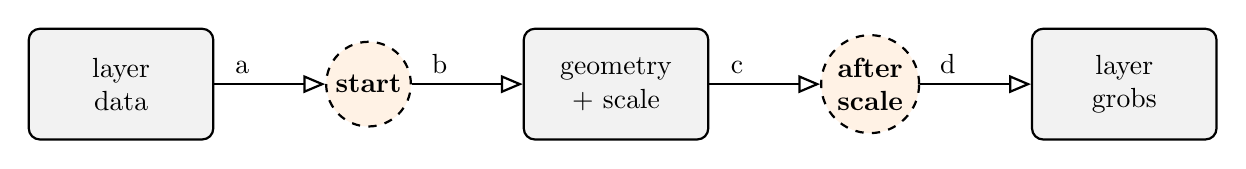
\begin{tikzpicture}[auto]
    \node [b] (data) {layer\\ data};
    \node [cc, right = of data] (mapping1) {\textbf{start}};
    \node [b, right = of mapping1] (geometry) {geometry + scale};
    \node [cc, right = of geometry] (mapping3) {\textbf{after\\ scale}};
    \node [b, right = of mapping3] (render) {layer\\ grobs};

    \path [ll] (mapping1) -- (data) node[near end,above]{a};
    \path [ll] (geometry) -- (mapping1) node[near end,above]{b};
    \path [ll] (mapping3) -- (geometry) node[near end,above]{c};
    \path [ll] (render) -- (mapping3) node[near end,above]{d};
  \end{tikzpicture}}}\hfill%
\vspace{2ex}

When a layer includes a statistics the data goes through three stages where mappings of variables to aesthetics can take place. As above we have \textbf{start} and \textbf{after scale}, but we have in addition \textbf{after stat}. Statistics compute new values from the data received as input and return them. These data become the input to the geometry after the \textbf{after stat} mapping stage.\vspace{2.5ex}

{\sffamily
\centering
\resizebox{\linewidth}{!}{%
  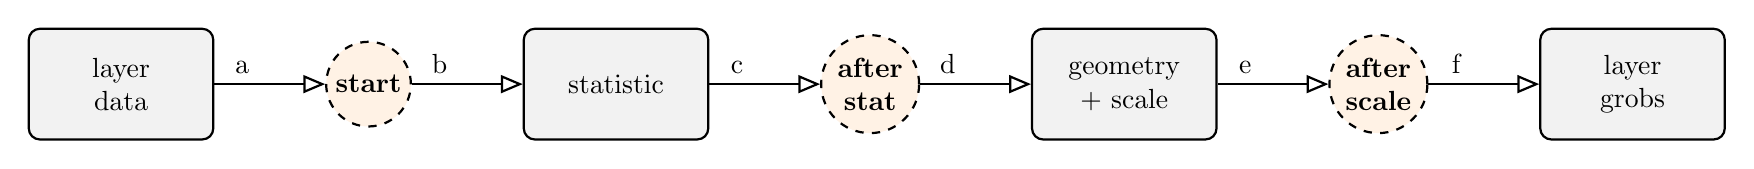
\begin{tikzpicture}[auto]
    \node [b] (data) {layer\\ data};
    \node [cc, right = of data] (mapping1) {\textbf{start}};
    \node [b, right = of mapping1] (statistic) {statistic};
    \node [cc, right = of statistic] (mapping2) {\textbf{after\\ stat}};
    \node [b, right = of mapping2] (geometry) {geometry + scale};
    \node [cc, right = of geometry] (mapping3) {\textbf{after\\ scale}};
    \node [b, right = of mapping3] (render) {layer\\ grobs};

    \path [ll] (mapping1) -- (data) node[near end,above]{a};
    \path [ll] (statistic) -- (mapping1) node[near end,above]{b};
    \path [ll] (mapping2) -- (statistic) node[near end,above]{c};
    \path [ll] (geometry) -- (mapping2) node[near end,above]{d};
    \path [ll] (mapping3) -- (geometry) node[near end,above]{e};
    \path [ll] (render) -- (mapping3) node[near end,above]{f};
  \end{tikzpicture}}}\vspace{2ex}

In more detail, a statistic receives as its input \code{data} mapped at the \textbf{start} as described in the previous example as received by the geometry. The statistic computes new values from the data. The computed values are returned by a statistics also as a data frame. This data frame contains different values, the number of rows and/or columns usually also differ from those in the data frame received as input. Statistics provide default mappings for the \textbf{after stat} stage and a default \code{geometry}, but these can be overridden by the user. Usually statistics return other variables in addition to those with default mappings to facilitate the constructions of variations on a given type of data summary. Within \Rfunction{aes()} we can use function \Rfunction{after\_stat()} to request a mapping after the statistic.

\begin{explainbox}
  In reality all ggplot layers include a statistic, but most geometries have \ggstat{stat\_identity()} as their default. There are some statistics that in \pkgname{ggplot2} have companion geometries that can be used interchangeably. This` tends to lead into confusion, and in this book, only geometries that have as default \ggstat{stat\_identity()} are described as geometries. In the case of those that by default use other statistics, like \gggeom{geom\_smooth()} I only describe the companion statistic, \gggeom{stat\_smooth()}.
\end{explainbox}

A ggplot can have a single layer or many layers, but when ggplots have more than one layer, the data flow, computations and generation of graphical objects takes place independently for each layer. As mentioned above, most ggplots do not have fully independent layers, but the layers share the same data and aesthetic mappings at the \textbf{start}. Ahead of this point computations in layers are always independent of those in other layers, except that for a given aesthetic only one scale is allowed per plot. This is intentional, and makes it nearly impossible for one aesthetic to be assigned different meanings in different layers of the same plot.
\index{grammar of graphics!plot workings|)}
\index{grammar of graphics!plot structure|)}

\subsection{Plot construction}
\index{grammar of graphics!plot construction|(}

As the use of the grammar is easier to demonstrate by example than to explain with words, I will show how to build plots of increasing complexity, starting from the simplest possible. All elements of a plot have defaults, although in some cases these defaults result in empty plots. Defaults make it possible to create a plot very succinctly. When building a plot step by step, we can consider the different aspects described in the previous section: the structure of the object, the graphic output, and the transformations applied to the data in the route between the recipe stored in an object and graphic output. In this section I emphasize the syntax of the grammar and how it translated into a plot.

\begin{advplayground}
  When reading this section, possibly a second time, use \code{summary()} and \code{str()} as described in the previous section to explore how \code{"gg"} plot objects gain new member components as the \emph{recipe} for the plot evolves in complexity.
\end{advplayground}

We start by using function \code{ggplot()} to create the skeleton for a plot, which can be enhanced, but also printed as is. \emph{A plot with no data or layers.}

\begin{knitrout}\footnotesize
\definecolor{shadecolor}{rgb}{0.969, 0.969, 0.969}\color{fgcolor}\begin{kframe}
\begin{alltt}
\hlkwd{ggplot}\hlstd{()}
\end{alltt}
\end{kframe}

{\centering 
\includegraphics[width=.7\textwidth]{figure/pos-ggplot-basics-01-1} 

}


\end{knitrout}

The plot above is of little use without any data, so we next pass a data frame object, in this case \code{mtcars}---\Rdata{mtcars} is a data set included in \Rlang; to learn more about this data set, type \code{help("mtcars")} at the \Rlang command prompt. Having no layers or scale, the result is also an empty grey plotting area. ({\small\textsf{data $\to$ \emph{ggplot object}}})

\begin{knitrout}\footnotesize
\definecolor{shadecolor}{rgb}{0.969, 0.969, 0.969}\color{fgcolor}\begin{kframe}
\begin{alltt}
\hlkwd{ggplot}\hlstd{(}\hlkwc{data} \hlstd{= mtcars)}
\end{alltt}
\end{kframe}
\end{knitrout}

Once the data are available, we need to select a graphical or geometric representation for the quantities to plot. The overall kind of representation is determined by the geometry, such as \code{geom\_point()} and \code{geom\_line()}, drawing separate points for the observations or connecting them with lines, respectively. A mapping indicates which property of the geometric elements will be used to represent the values stored in a given variable in the user's data. For most geometries we need to provide mappings for both $x$ and $y$ aesthetics, to establish the position of the geometrical shapes like points or lines in the plotting area. Additional aesthetics like colour (applicable to both points and lines) or shape and linetype, applicable to points and lines, respectively have default mappings. Defaults can be overridden by including a mapping explicitly in the call to \code{aes()}.

Here we map at the \textbf{start} stage two variables in the data, \code{disp} to $x$ and and \code{mpg} to $y$ aesthetics. This mapping can be seen in the chunk below by its effect on the plotting area ranges that now match the ranges of the mapped variables, expanded by a small margin. The axis labels also reflect the names of the mapped variables, however, there is no graphical element yet displayed for the individual observations. ({\small\textsf{data $\to$ aes $\to$ \emph{ggplot object}}})

\begin{knitrout}\footnotesize
\definecolor{shadecolor}{rgb}{0.969, 0.969, 0.969}\color{fgcolor}\begin{kframe}
\begin{alltt}
\hlkwd{ggplot}\hlstd{(}\hlkwc{data} \hlstd{= mtcars,}
       \hlkwd{aes}\hlstd{(}\hlkwc{x} \hlstd{= disp,} \hlkwc{y} \hlstd{= mpg))}
\end{alltt}
\end{kframe}

{\centering 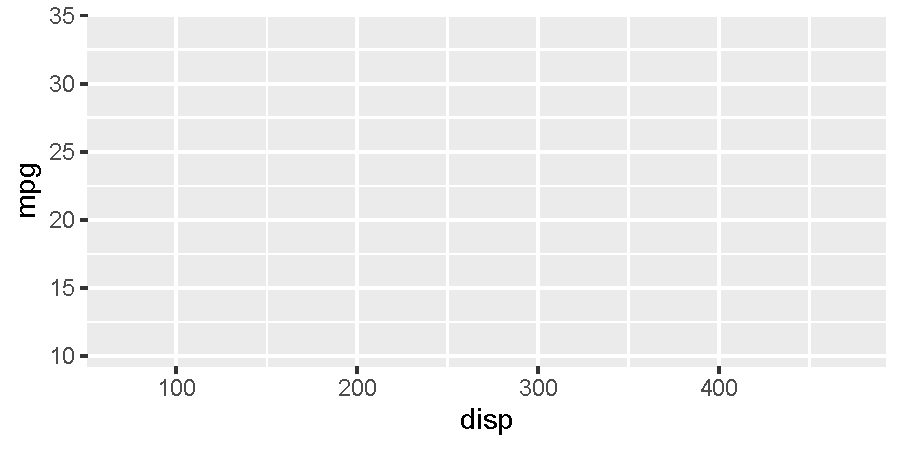
\includegraphics[width=.7\textwidth]{figure/pos-ggplot-basics-03-1} 

}


\end{knitrout}

To make observations visible we need to add a suitable \emph{geometry} or \code{geom} to the plot recipe. Here we display the observations as points using \gggeom{geom\_point()}, i.e, we add a \emph{plot layer}. ({\small\textsf{data $\to$ aes $\to$ geom $\to$ \emph{ggplot object}}})

\begin{knitrout}\footnotesize
\definecolor{shadecolor}{rgb}{0.969, 0.969, 0.969}\color{fgcolor}\begin{kframe}
\begin{alltt}
\hlkwd{ggplot}\hlstd{(}\hlkwc{data} \hlstd{= mtcars,}
       \hlkwd{aes}\hlstd{(}\hlkwc{x} \hlstd{= disp,} \hlkwc{y} \hlstd{= mpg))} \hlopt{+}
  \hlkwd{geom_point}\hlstd{()}
\end{alltt}
\end{kframe}

{\centering 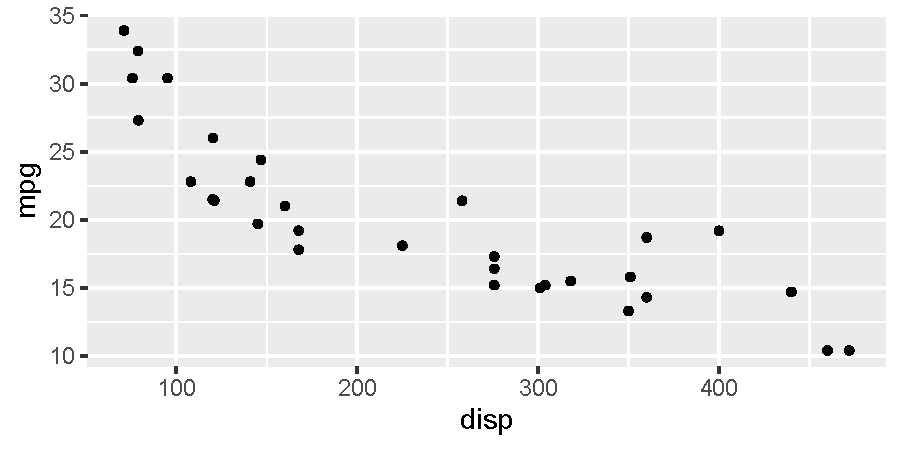
\includegraphics[width=.7\textwidth]{figure/pos-ggplot-basics-04-1} 

}


\end{knitrout}

\begin{warningbox}
In the examples above, the plots were printed automatically, which is the default at the \Rlang console. However, as with other \Rlang objects, ggplots can be assigned to a variable as first shown in section \ref{sec:plot:workings} on page \pageref{sec:plot:workings}.

\begin{knitrout}\footnotesize
\definecolor{shadecolor}{rgb}{0.969, 0.969, 0.969}\color{fgcolor}\begin{kframe}
\begin{alltt}
\hlstd{p} \hlkwb{<-} \hlkwd{ggplot}\hlstd{(}\hlkwc{data} \hlstd{= mtcars,}
            \hlkwd{aes}\hlstd{(}\hlkwc{x} \hlstd{= disp,} \hlkwc{y} \hlstd{= mpg))} \hlopt{+}
       \hlkwd{geom_point}\hlstd{()}
\end{alltt}
\end{kframe}
\end{knitrout}

and printed at a later time, and saved to and read from files on disk.

\begin{knitrout}\footnotesize
\definecolor{shadecolor}{rgb}{0.969, 0.969, 0.969}\color{fgcolor}\begin{kframe}
\begin{alltt}
\hlkwd{print}\hlstd{(p)}
\end{alltt}
\end{kframe}
\end{knitrout}

Layers and other elements can be also added to a saved ggplot as the saved objects are not the graphical representation of the plots themselves but instead a \emph{recipe} plus data needed to build them.
\end{warningbox}

\begin{advplayground}
Above we have seen how to build a plot and we also had a glimpse of the structure of a simple \code{"gg"} plot object. We have also saved a ggplot under the name \code{p}.

We can view the structure of any R object, including \code{"gg"} plot objects,  with \code{str()}. Package \pkgname{ggplot2} provides a \code{summary()} for \code{"gg"} plot object. Package \pkgname{gginnards} provides methods \code{str()}, \code{num\_layers()}, \code{top\_layer()}, \code{bottom\_layer()}, and \code{mapped\_vars()}. As you make progress through the chapter, use these methods to explore \code{"gg"} plot objects with different numbers of layers or mappings. You will be able to see how the plot components are stored as members of the \code{"gg"} plot objects.
\end{advplayground}

Although \emph{aesthetics} are usually mapped to variables in the data, they can also be set to constant values, as many of them are by default. While variables in \code{data} can be both mapped using \code{aes()} as whole-plot defaults, as shown above, or within individual layers, constant values for aesthetics can be set, as shown here, only for individual layers and directly rather than using \code{aes()}.

\begin{knitrout}\footnotesize
\definecolor{shadecolor}{rgb}{0.969, 0.969, 0.969}\color{fgcolor}\begin{kframe}
\begin{alltt}
\hlkwd{ggplot}\hlstd{(}\hlkwc{data} \hlstd{= mtcars,}
       \hlkwd{aes}\hlstd{(}\hlkwc{x} \hlstd{= disp,} \hlkwc{y} \hlstd{= mpg))} \hlopt{+}
  \hlkwd{geom_point}\hlstd{(}\hlkwc{color} \hlstd{=} \hlstr{"red"}\hlstd{,} \hlkwc{shape} \hlstd{=} \hlstr{"square"}\hlstd{)}
\end{alltt}
\end{kframe}

{\centering 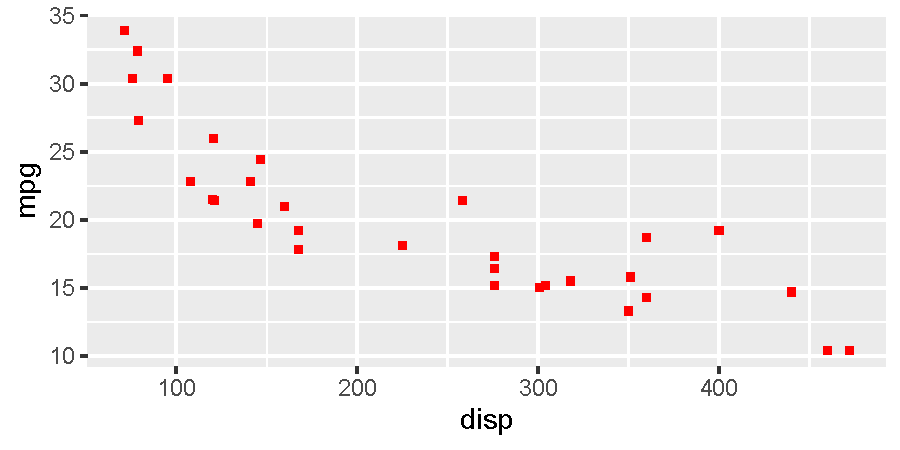
\includegraphics[width=.7\textwidth]{figure/pos-ggplot-basics-04a-1} 

}


\end{knitrout}

While a geometry directly constructs during rendering a graphical representation of the observations or summaries in the data it receives as input, a \emph{statistics} or \code{stat} ``sits'' in-between the data and a \code{geom}, applying some computation, usually but not always, to produce a statistical summary of the data. Here we add a fitted line using \code{stat\_smooth()} with its output added to the plot using \gggeom{geom\_line()} passed by name with \code{"line"} as an argument to \code{stat\_smooth()}. We fit a linear regression, using \code{lm()} as the method. This plot has two layers, from geometries \gggeom{geom\_point()} and \gggeom{geom\_line()}. ({\small\textsf{data $\to$ aes $\to$ stat $\to$ geom $\to$ \emph{ggplot object}}})

\begin{knitrout}\footnotesize
\definecolor{shadecolor}{rgb}{0.969, 0.969, 0.969}\color{fgcolor}\begin{kframe}
\begin{alltt}
\hlkwd{ggplot}\hlstd{(}\hlkwc{data} \hlstd{= mtcars,}
       \hlkwd{aes}\hlstd{(}\hlkwc{x} \hlstd{= disp,} \hlkwc{y} \hlstd{= mpg))} \hlopt{+}
  \hlkwd{geom_point}\hlstd{()} \hlopt{+}
  \hlkwd{stat_smooth}\hlstd{(}\hlkwc{geom} \hlstd{=} \hlstr{"line"}\hlstd{,} \hlkwc{method} \hlstd{=} \hlstr{"lm"}\hlstd{,} \hlkwc{formula} \hlstd{= y} \hlopt{~} \hlstd{x)}
\end{alltt}
\end{kframe}

{\centering 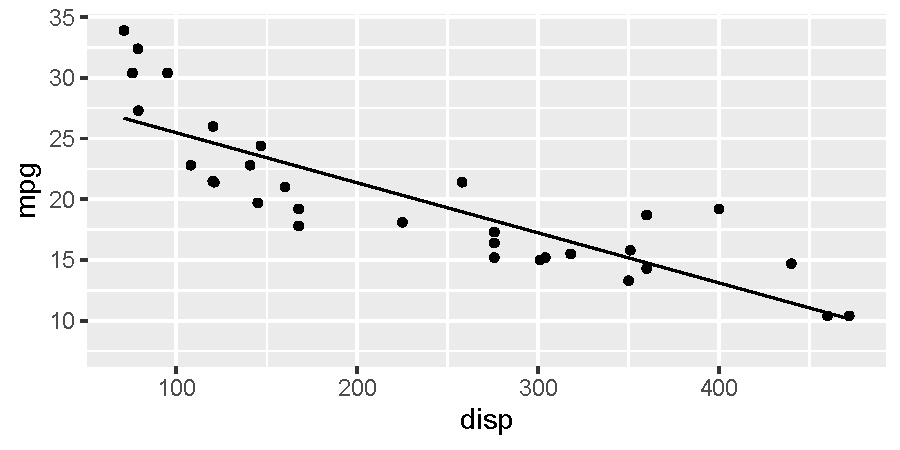
\includegraphics[width=.7\textwidth]{figure/pos-ggplot-basics-05-1} 

}


\end{knitrout}

We haven't yet added some of the elements of the grammar described above: \emph{scales}, \emph{coordinates} and \emph{themes}. The plots were rendered anyway because these elements have defaults which are used when we do not set them explicitly. We next will see examples in which they are explicitly set. We start with a scale using a logarithmic transformation. This works like plotting by hand using graph paper with rulings spaced according to a logarithmic scale. Tick marks continue to be expressed in the original units, but statistics are applied to the transformed data. In other words, a transformed scale affects the values before they are passed to \emph{statistics}, and the linear regression will be fitted to \code{log10()} transformed $y$ values and the original $x$ values. ({\small\textsf{data $\to$ aes $\to$ stat $\to$ geom $\to$ scale $\to$ \emph{ggplot object}}})

\begin{knitrout}\footnotesize
\definecolor{shadecolor}{rgb}{0.969, 0.969, 0.969}\color{fgcolor}\begin{kframe}
\begin{alltt}
\hlkwd{ggplot}\hlstd{(}\hlkwc{data} \hlstd{= mtcars,}
       \hlkwd{aes}\hlstd{(}\hlkwc{x} \hlstd{= disp,} \hlkwc{y} \hlstd{= mpg))} \hlopt{+}
  \hlkwd{geom_point}\hlstd{()} \hlopt{+}
  \hlkwd{stat_smooth}\hlstd{(}\hlkwc{geom} \hlstd{=} \hlstr{"line"}\hlstd{,} \hlkwc{method} \hlstd{=} \hlstr{"lm"}\hlstd{,} \hlkwc{formula} \hlstd{= y} \hlopt{~} \hlstd{x)} \hlopt{+}
  \hlkwd{scale_y_log10}\hlstd{()}
\end{alltt}
\end{kframe}

{\centering 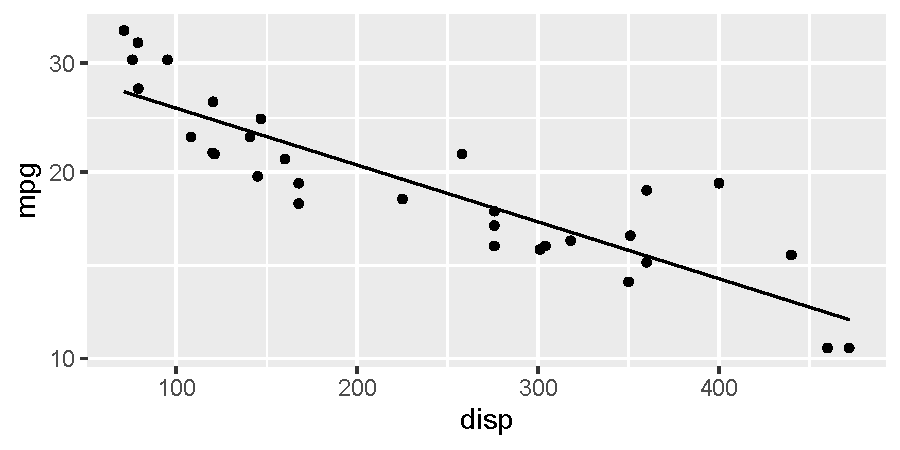
\includegraphics[width=.7\textwidth]{figure/pos-ggplot-basics-06-1} 

}


\end{knitrout}

The range limits of a scale can be set manually, instead of automatically as by default. These limits create a virtual \emph{window into the data}: out-of-bounds (oob) observations, those outside the scale limits remain hidden and are not mapped to aesthetics---i.e., these observations are not included in the graphical representation or used in calculations. Crucially, when using \emph{statistics} the computations are only applied to observations that fall within the limits of all scales in use. These limits \emph{indirectly} affect the plotting area when the plotting area is automatically set based on the range of the (within limits) data---even the mapping to values of a different aesthetics may change when a subset of the data are selected by manually setting the limits of a scale.

In contrast to \emph{scale limits}, \emph{coordinates}\index{grammar of graphics!cartesian coordinates} function as a \emph{zoomed view} into the plotting area, and do not affect which observations are visible to \emph{statistics}. The coordinate system, as expected, is also determined by this grammar element---here we use cartesian coordinates which are the default, but we manually set $y$ limits. ({\small\textsf{data $\to$ aes $\to$ stat $\to$ geom $\to$ coordinate $\to$ theme $\to$ \emph{ggplot object}}})

\begin{knitrout}\footnotesize
\definecolor{shadecolor}{rgb}{0.969, 0.969, 0.969}\color{fgcolor}\begin{kframe}
\begin{alltt}
\hlkwd{ggplot}\hlstd{(}\hlkwc{data} \hlstd{= mtcars,}
       \hlkwd{aes}\hlstd{(}\hlkwc{x} \hlstd{= disp,} \hlkwc{y} \hlstd{= mpg))} \hlopt{+}
  \hlkwd{geom_point}\hlstd{()} \hlopt{+}
  \hlkwd{stat_smooth}\hlstd{(}\hlkwc{geom} \hlstd{=} \hlstr{"line"}\hlstd{,} \hlkwc{method} \hlstd{=} \hlstr{"lm"}\hlstd{,} \hlkwc{formula} \hlstd{= y} \hlopt{~} \hlstd{x)} \hlopt{+}
  \hlkwd{coord_cartesian}\hlstd{(}\hlkwc{ylim} \hlstd{=} \hlkwd{c}\hlstd{(}\hlnum{15}\hlstd{,} \hlnum{25}\hlstd{))}
\end{alltt}
\end{kframe}

{\centering 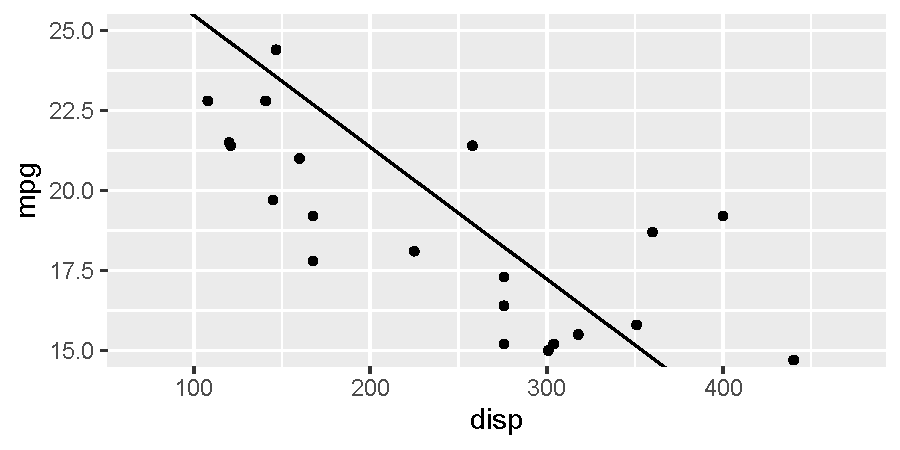
\includegraphics[width=.7\textwidth]{figure/pos-ggplot-basics-07-1} 

}


\end{knitrout}

The next example uses a coordinate system transformation. When the transformation is applied to the coordinate system, it affects only the plotting---it sits between the \code{geom} and the rendering of the plot. The transformation is applied to the values returned by any \emph{statistics}. The straight line fitted is plotted on the transformed coordinates as a curve, because the model was fitted to the untransformed data and this fitted model is automatically used to obtain the predicted values, which are then plotted after the transformation is applied to them. We have here described only cartesian coordinate systems while other coordinate systems are described in sections \ref{sec:plot:sf} and \ref{sec:plot:circular} on pages \pageref{sec:plot:sf} and \pageref{sec:plot:circular}, respectively.

\begin{knitrout}\footnotesize
\definecolor{shadecolor}{rgb}{0.969, 0.969, 0.969}\color{fgcolor}\begin{kframe}
\begin{alltt}
\hlkwd{ggplot}\hlstd{(}\hlkwc{data} \hlstd{= mtcars,}
       \hlkwd{aes}\hlstd{(}\hlkwc{x} \hlstd{= disp,} \hlkwc{y} \hlstd{= mpg))} \hlopt{+}
  \hlkwd{geom_point}\hlstd{()} \hlopt{+}
  \hlkwd{stat_smooth}\hlstd{(}\hlkwc{geom} \hlstd{=} \hlstr{"line"}\hlstd{,} \hlkwc{method} \hlstd{=} \hlstr{"lm"}\hlstd{,} \hlkwc{formula} \hlstd{= y} \hlopt{~} \hlstd{x)} \hlopt{+}
  \hlkwd{coord_trans}\hlstd{(}\hlkwc{y} \hlstd{=} \hlstr{"log10"}\hlstd{)}
\end{alltt}
\end{kframe}

{\centering 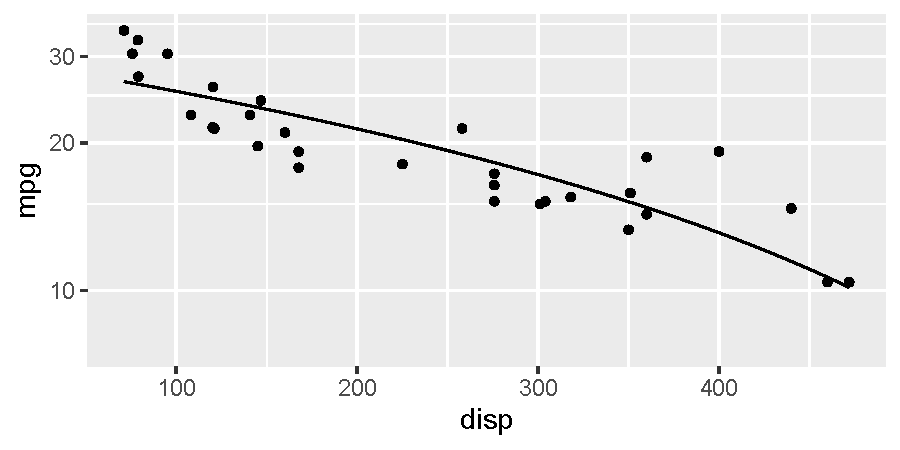
\includegraphics[width=.7\textwidth]{figure/pos-ggplot-basics-08-1} 

}


\end{knitrout}

Themes affect the rendering of plots at the time of printing---they can be thought of as style sheets defining the graphic design. A complete theme can override the default gray theme. The plot is the same, the observations are represented in the same way, the limits of the axes are the same and all text is the same. On the other, hand how these elements are rendered by different themes can be drastically different. ({\small\textsf{data $\to$ aes $\to$ $\to$ geom $\to$ theme $\to$ \emph{ggplot object}}}

\begin{knitrout}\footnotesize
\definecolor{shadecolor}{rgb}{0.969, 0.969, 0.969}\color{fgcolor}\begin{kframe}
\begin{alltt}
\hlkwd{ggplot}\hlstd{(}\hlkwc{data} \hlstd{= mtcars,}
       \hlkwd{aes}\hlstd{(}\hlkwc{x} \hlstd{= disp,} \hlkwc{y} \hlstd{= mpg))} \hlopt{+}
  \hlkwd{geom_point}\hlstd{()} \hlopt{+}
  \hlkwd{theme_classic}\hlstd{()}
\end{alltt}
\end{kframe}

{\centering 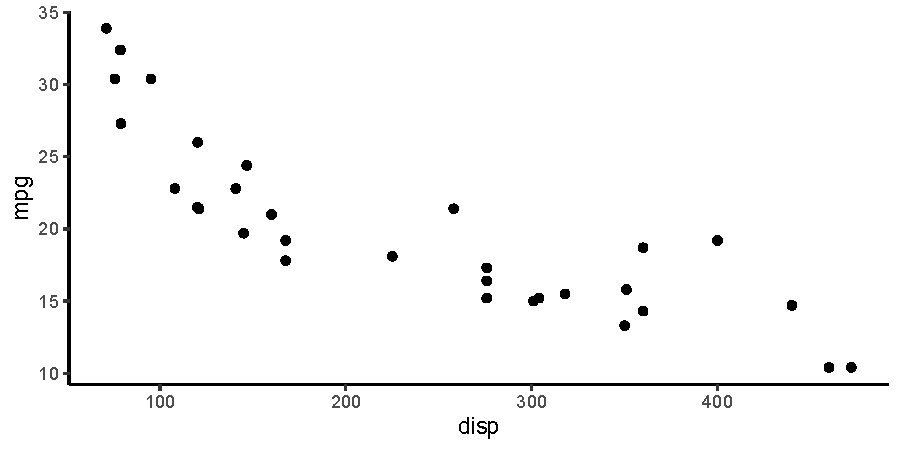
\includegraphics[width=.7\textwidth]{figure/pos-ggplot-basics-09-1} 

}


\end{knitrout}

We can also override the base font size and font family. This affects the size of all text elements, as their size is defined relative to the base size. Here we add the same theme as used in the previous example, but with a different base point size for text.

\begin{knitrout}\footnotesize
\definecolor{shadecolor}{rgb}{0.969, 0.969, 0.969}\color{fgcolor}\begin{kframe}
\begin{alltt}
\hlkwd{ggplot}\hlstd{(}\hlkwc{data} \hlstd{= mtcars,}
       \hlkwd{aes}\hlstd{(}\hlkwc{x} \hlstd{= disp,} \hlkwc{y} \hlstd{= mpg))} \hlopt{+}
  \hlkwd{geom_point}\hlstd{()} \hlopt{+}
  \hlkwd{theme_classic}\hlstd{(}\hlkwc{base_size} \hlstd{=} \hlnum{20}\hlstd{,} \hlkwc{base_family} \hlstd{=} \hlstr{"serif"}\hlstd{)}
\end{alltt}
\end{kframe}

{\centering 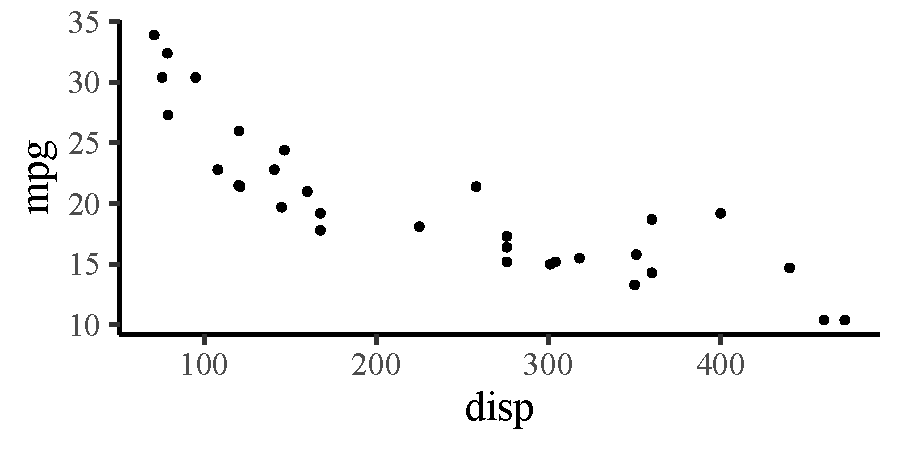
\includegraphics[width=.7\textwidth]{figure/pos-ggplot-basics-10-1} 

}


\end{knitrout}

The details of how to set axis labels, tick positions and tick labels will be discussed in depth in section \ref{sec:plot:scales}. Meanwhile, we will use function \code{labs()} which is \emph{a convenience function} allowing us to easily set the title and subtitle of a plot and to replace the default \code{name} of scales, in this case, those used for axis labels---by default the \code{name} of scales is set to the name of the mapped variable. When setting the \code{name} of scales with \code{labs()}, we use as parameter names in the function call the names of aesthetics and pass as an argument a character string, or an \Rlang expression. Here we use \code{x} and \code{y}, the names of the two \emph{aesthetics} to which we have mapped two variables in \code{data}, \code{disp} and \code{mpg}.

\begin{knitrout}\footnotesize
\definecolor{shadecolor}{rgb}{0.969, 0.969, 0.969}\color{fgcolor}\begin{kframe}
\begin{alltt}
\hlkwd{ggplot}\hlstd{(}\hlkwc{data} \hlstd{= mtcars,}
       \hlkwd{aes}\hlstd{(}\hlkwc{x} \hlstd{= disp,} \hlkwc{y} \hlstd{= mpg))} \hlopt{+}
  \hlkwd{geom_point}\hlstd{()} \hlopt{+}
  \hlkwd{labs}\hlstd{(}\hlkwc{x} \hlstd{=} \hlstr{"Engine displacement (cubic inches)"}\hlstd{,}
       \hlkwc{y} \hlstd{=} \hlstr{"Fuel use efficiency\textbackslash{}n(miles per gallon)"}\hlstd{,}
       \hlkwc{title} \hlstd{=} \hlstr{"Motor Trend Car Road Tests"}\hlstd{,}
       \hlkwc{subtitle} \hlstd{=} \hlstr{"Source: 1974 Motor Trend US magazine"}\hlstd{)}
\end{alltt}
\end{kframe}

{\centering 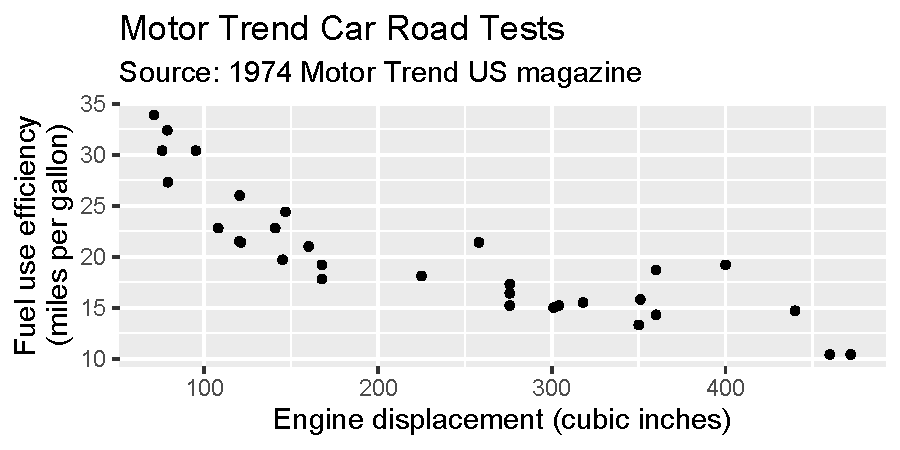
\includegraphics[width=.7\textwidth]{figure/pos-ggplot-basics-11-1} 

}


\end{knitrout}

\begin{infobox}
As elsewhere in \Rlang, when a value is expected, either a value stored in a variable or a more complex statement returning a suitable value can be passed as an argument to be mapped to an \emph{aesthetic}. In other words, the values to be plotted do not need to be stored as variables (or columns) in the data frame passed as an argument to parameter \code{data}, they can also be computed from these variables. Here we plot miles-per-gallon, \code{mpg} on the engine displacement per cylinder by dividing \code{disp} by \code{cyl} within the call to \code{aes()}.

\begin{knitrout}\footnotesize
\definecolor{shadecolor}{rgb}{0.969, 0.969, 0.969}\color{fgcolor}\begin{kframe}
\begin{alltt}
\hlkwd{ggplot}\hlstd{(}\hlkwc{data} \hlstd{= mtcars,} \hlkwd{aes}\hlstd{(}\hlkwc{x} \hlstd{= disp} \hlopt{/} \hlstd{cyl,} \hlkwc{y} \hlstd{= mpg))} \hlopt{+}
  \hlkwd{geom_point}\hlstd{()}
\end{alltt}
\end{kframe}

{\centering 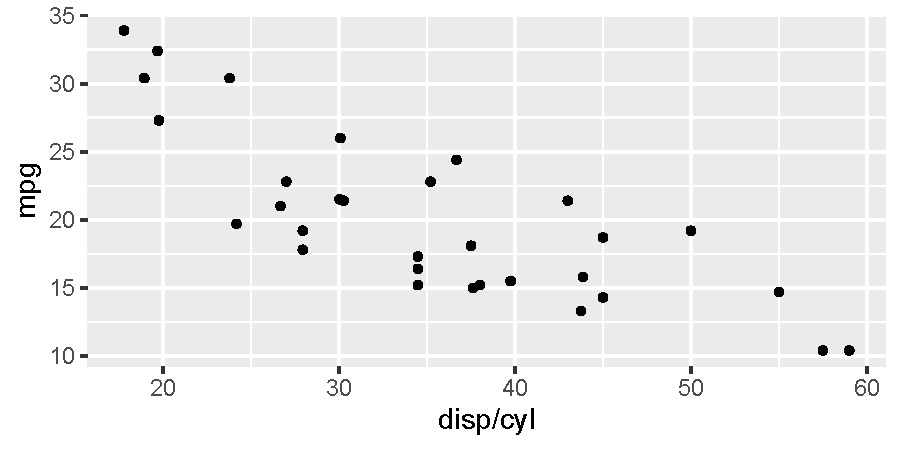
\includegraphics[width=.7\textwidth]{figure/pos-ggplot-basics-info-01-1} 

}


\end{knitrout}

\end{infobox}

We can summarize the data transformation steps described above as a linear chain:
{\small\textsf{data $\to$ aes $\to$ stat $\to$ aes $\to$ geom $\to$ scale $\to$ aes $\to$ coordinate $\to$ theme $\to$ \emph{ggplot object}}}

Each of the elements of the grammar exemplified above has several different member functions, and many of the individual \emph{geometries} and \emph{statistics} accept arguments that can be used to modify their behavior. There are also more \emph{aesthetics} than those shown above. Multiple data objects as well as multiple mappings can coexist within a single \code{"gg"} plot object. Packages and user code can define new \emph{geometries}, \emph{statistics}, \emph{coordinates} and even implement new \emph{aesthetics}. Being \Rmethod{ggplot()} an S3 method, specializations for objects of classes different from \code{data.frame} exist. Individual elements in a theme can also be modified and new complete themes created, re-used and shared. We will describe in the remaining sections of this chapter how to use the grammar of graphics to construct other types of graphical presentations including more complex plots than those in the examples above.
\index{grammar of graphics!plot construction|)}

\subsection{Plots as \Rlang objects}
\index{grammar of graphics!plots as R objects|(}
We can manipulate \code{"gg"} plot objects and their components in the same way as other \Rlang objects. We can operate on them using the operators and methods defined for the \code{"gg"} class they belong to. We start by saving a ggplot into a variable.

\begin{knitrout}\footnotesize
\definecolor{shadecolor}{rgb}{0.969, 0.969, 0.969}\color{fgcolor}\begin{kframe}
\begin{alltt}
\hlstd{p} \hlkwb{<-} \hlkwd{ggplot}\hlstd{(}\hlkwc{data} \hlstd{= mtcars,}
       \hlkwd{aes}\hlstd{(}\hlkwc{x} \hlstd{= disp,} \hlkwc{y} \hlstd{= mpg))} \hlopt{+}
  \hlkwd{geom_point}\hlstd{()}
\end{alltt}
\end{kframe}
\end{knitrout}

\begin{warningbox}
  \index{grammar of graphics!structure of plot objects|(}
  The separation of plot construction and rendering is possible, because \code{"gg"} objects are self-contained. Most importantly, a copy of the data object passed as argument is saved within the plot object. In the example above, \code{p} by itself could be saved to a file on disk and loaded into a clean \Rlang session, even on another computer, and rendered as long as package \ggplot and its dependencies are available. Another consequence of storing a copy of the data in the plot object, is that editing after the creation of a \code{"gg"} object the data frame passed as argument to \code{data} when it was created does \emph{not} get reflected in newly rendered plots unless we recreate the "gg" object.

  With \code{str()} we can explore the structure of any \Rlang object, including those of class \code{"gg"}. We use \code{max.level = 1} to reduce the length of output, but to see deeper into the nested list you can increase the value passed as an argument to \code{max.level} or simply accept its default.

% the next chuck works but it leads to stack overflow in LaTeX
% there is something wrong with how knitr handles the output of str()
% eval_playground
\begin{knitrout}\footnotesize
\definecolor{shadecolor}{rgb}{0.969, 0.969, 0.969}\color{fgcolor}\begin{kframe}
\begin{alltt}
\hlkwd{str}\hlstd{(p,} \hlkwc{max.level} \hlstd{=} \hlnum{1}\hlstd{)}
\end{alltt}
\end{kframe}
\end{knitrout}
  \index{grammar of graphics!structure of plot objects|)}
\end{warningbox}

When we used in the previous section operator \code{+} to assemble the plots, we were operating on ``anonymous'' \Rlang objects. In the same way, we can operate on saved or ``named'' objects.

\begin{knitrout}\footnotesize
\definecolor{shadecolor}{rgb}{0.969, 0.969, 0.969}\color{fgcolor}\begin{kframe}
\begin{alltt}
\hlstd{p} \hlopt{+}
  \hlkwd{stat_smooth}\hlstd{(}\hlkwc{geom} \hlstd{=} \hlstr{"line"}\hlstd{,} \hlkwc{method} \hlstd{=} \hlstr{"lm"}\hlstd{,} \hlkwc{formula} \hlstd{= y} \hlopt{~} \hlstd{x)}
\end{alltt}
\end{kframe}

{\centering 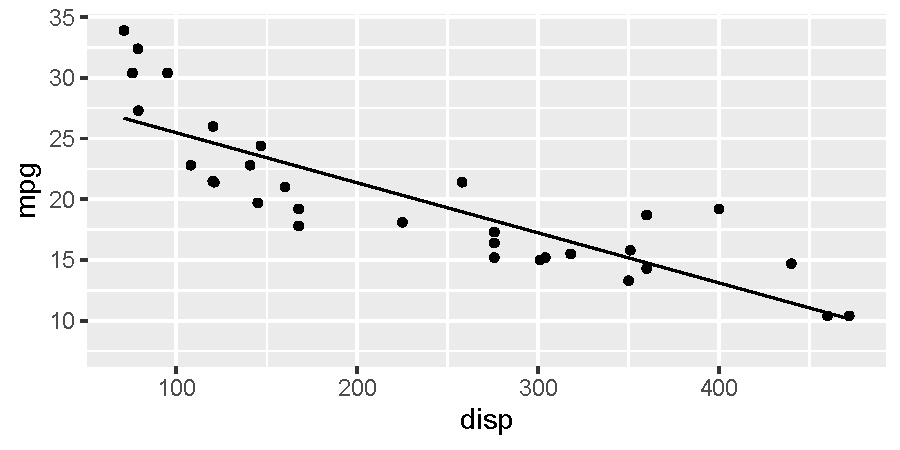
\includegraphics[width=.7\textwidth]{figure/pos-ggplot-objects-02-1} 

}


\end{knitrout}

\begin{playground}
  Reproduce the examples in the previous section, using \code{p} defined above as a basis instead of building each plot from scratch.
\end{playground}

\begin{infobox}
  In the examples above we have been adding elements one by one, using the \code{+} operator. It is also possible to add multiple components in a single operation using a list. This is useful, when we want to save sets of components in a variable so as to reuse them in multiple plots. This saves typing, ensures consistency and can make alterations to a set of similar plots much easier.

\begin{knitrout}\footnotesize
\definecolor{shadecolor}{rgb}{0.969, 0.969, 0.969}\color{fgcolor}\begin{kframe}
\begin{alltt}
\hlstd{my.layer} \hlkwb{<-} \hlkwd{list}\hlstd{(}
  \hlkwd{stat_smooth}\hlstd{(}\hlkwc{geom} \hlstd{=} \hlstr{"line"}\hlstd{,} \hlkwc{method} \hlstd{=} \hlstr{"lm"}\hlstd{,} \hlkwc{formula} \hlstd{= y} \hlopt{~} \hlstd{x),}
  \hlkwd{scale_x_log10}\hlstd{())}
\end{alltt}
\end{kframe}
\end{knitrout}

\begin{knitrout}\footnotesize
\definecolor{shadecolor}{rgb}{0.969, 0.969, 0.969}\color{fgcolor}\begin{kframe}
\begin{alltt}
\hlstd{p} \hlopt{+} \hlstd{my.layer}
\end{alltt}
\end{kframe}

{\centering 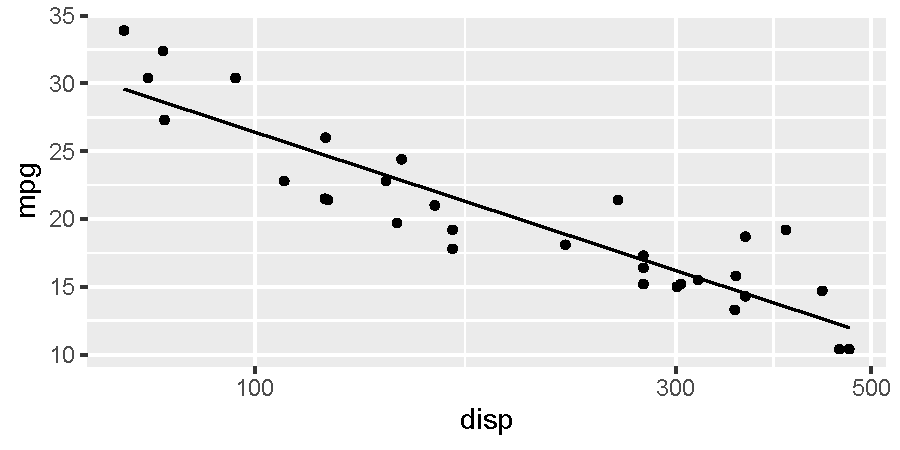
\includegraphics[width=.7\textwidth]{figure/pos-ggplot-objects-info-02-1} 

}


\end{knitrout}

\end{infobox}
\index{grammar of graphics!plots as R objects|)}

\subsection{Mappings in detail}
\index{grammar of graphics!mapping of data|(}
\index{grammar of graphics!aesthetics(}
In the case of simple plots, based on data contained in a single data frame, the usual style is to code a plot as described above, passing an argument, \code{mtcars} in these examples, to the \code{data} parameter of \Rfunction{ggplot()}. Data passed in this way becomes the default for all layers in the plot. The same applies to the argument passed to \code{mapping}.\qRfunction{aes()}

\begin{knitrout}\footnotesize
\definecolor{shadecolor}{rgb}{0.969, 0.969, 0.969}\color{fgcolor}\begin{kframe}
\begin{alltt}
\hlkwd{ggplot}\hlstd{(}\hlkwc{data} \hlstd{= mtcars,}
       \hlkwc{mapping} \hlstd{=} \hlkwd{aes}\hlstd{(}\hlkwc{x} \hlstd{= disp,} \hlkwc{y} \hlstd{= mpg))} \hlopt{+}
  \hlkwd{geom_point}\hlstd{()}
\end{alltt}
\end{kframe}
\end{knitrout}

However, the grammar of graphics contemplates the possibility of data and mappings restricted to individual layers, passed to statistics or geometries through their \code{mapping} formal parameter. In this case, those mappings set in the call to \Rfunction{ggplot()}, if present,  are overridden by arguments passed to individual layers, making it possible to code the same plot as follows.

\begin{knitrout}\footnotesize
\definecolor{shadecolor}{rgb}{0.969, 0.969, 0.969}\color{fgcolor}\begin{kframe}
\begin{alltt}
\hlkwd{ggplot}\hlstd{()} \hlopt{+}
  \hlkwd{geom_point}\hlstd{(}\hlkwc{data} \hlstd{= mtcars,}
             \hlkwc{mapping} \hlstd{=} \hlkwd{aes}\hlstd{(}\hlkwc{x} \hlstd{= disp,} \hlkwc{y} \hlstd{= mpg))}
\end{alltt}
\end{kframe}
\end{knitrout}

\begin{explainbox}
The two examples show the two most commonly used styles when working at the console or writing simple scripts. There are other possibilities which are most useful when writing complex scripts, or in function definitions. We gui
The default mapping can also be added directly with the \code{+} operator, instead of being passed as an argument to \Rfunction{ggplot()}.

\begin{knitrout}\footnotesize
\definecolor{shadecolor}{rgb}{0.969, 0.969, 0.969}\color{fgcolor}\begin{kframe}
\begin{alltt}
\hlkwd{ggplot}\hlstd{(}\hlkwc{data} \hlstd{= mtcars)} \hlopt{+}
  \hlkwd{aes}\hlstd{(}\hlkwc{x} \hlstd{= disp,} \hlkwc{y} \hlstd{= mpg)} \hlopt{+}
  \hlkwd{geom_point}\hlstd{()}
\end{alltt}
\end{kframe}
\end{knitrout}

It is also possible to have a default mapping for the whole plot, but no default data.

\begin{knitrout}\footnotesize
\definecolor{shadecolor}{rgb}{0.969, 0.969, 0.969}\color{fgcolor}\begin{kframe}
\begin{alltt}
\hlkwd{ggplot}\hlstd{()} \hlopt{+}
  \hlkwd{aes}\hlstd{(}\hlkwc{x} \hlstd{= disp,} \hlkwc{y} \hlstd{= mpg)} \hlopt{+}
  \hlkwd{geom_point}\hlstd{(}\hlkwc{data} \hlstd{= mtcars)}
\end{alltt}
\end{kframe}
\end{knitrout}

We can save the mapping to a variable and add the variable instead of the call to \code{aes()} in each of the examples above, of which we show only the first one.

\begin{knitrout}\footnotesize
\definecolor{shadecolor}{rgb}{0.969, 0.969, 0.969}\color{fgcolor}\begin{kframe}
\begin{alltt}
\hlstd{my.mapping} \hlkwb{<-} \hlkwd{aes}\hlstd{(}\hlkwc{x} \hlstd{= disp,} \hlkwc{y} \hlstd{= mpg)}
\hlkwd{ggplot}\hlstd{(}\hlkwc{data} \hlstd{= mtcars,}
       \hlkwc{mapping} \hlstd{= my.mapping)} \hlopt{+}
  \hlkwd{geom_point}\hlstd{()}
\end{alltt}
\end{kframe}
\end{knitrout}

In all these examples, the plot remains unchanged (not shown). However, this flexibility in the grammar allows, as discussed in section \ref{sec:plot:workings} on \pageref{sec:plot:workings} makes it possible for layers to remain independent of each other when needed.
\end{explainbox}

The argument passed to parameter \code{data} of a layer function, can be a function instead of a data frame if the plot contains default data. In this case, the function is applied to the default data and must return a data frame containing data to be used in the layer. Here I use an anonymous function defined in-line, but a function can also be passed as argument by name.

\begin{knitrout}\footnotesize
\definecolor{shadecolor}{rgb}{0.969, 0.969, 0.969}\color{fgcolor}\begin{kframe}
\begin{alltt}
\hlkwd{ggplot}\hlstd{(}\hlkwc{data} \hlstd{= mtcars,}
       \hlkwc{mapping} \hlstd{=} \hlkwd{aes}\hlstd{(}\hlkwc{x} \hlstd{= disp,} \hlkwc{y} \hlstd{= mpg))} \hlopt{+}
  \hlkwd{geom_point}\hlstd{(}\hlkwc{size} \hlstd{=} \hlnum{4}\hlstd{)} \hlopt{+}
  \hlkwd{geom_point}\hlstd{(}\hlkwc{data} \hlstd{=} \hlkwa{function}\hlstd{(}\hlkwc{x}\hlstd{)\{}\hlkwd{subset}\hlstd{(x, cyl} \hlopt{==} \hlnum{4}\hlstd{)\},} \hlkwc{color} \hlstd{=} \hlstr{"yellow"}\hlstd{,}
             \hlkwc{size} \hlstd{=} \hlnum{1.5}\hlstd{)}
\end{alltt}
\end{kframe}
\end{knitrout}

The plot's default data can also be operated upon using the \pkgname{magritrr} pipe operator, but not the pipe operator native to \Rlang (\Roperator{|>}) or the dot-pipe operator from \pkgname{wrapr} (see section \ref{sec:data:pipes} on page \pageref{sec:data:pipes}). Using a function as above is simpler and clearer.
\begin{knitrout}\footnotesize
\definecolor{shadecolor}{rgb}{0.969, 0.969, 0.969}\color{fgcolor}\begin{kframe}
\begin{alltt}
\hlkwd{ggplot}\hlstd{(}\hlkwc{data} \hlstd{= mtcars,}
       \hlkwc{mapping} \hlstd{=} \hlkwd{aes}\hlstd{(}\hlkwc{x} \hlstd{= disp,} \hlkwc{y} \hlstd{= mpg))} \hlopt{+}
  \hlkwd{geom_point}\hlstd{(}\hlkwc{size} \hlstd{=} \hlnum{4}\hlstd{)} \hlopt{+}
  \hlkwd{geom_point}\hlstd{(}\hlkwc{data} \hlstd{= .} \hlopt \hlkwd{subset}\hlstd{(}\hlkwc{x} \hlstd{= ., cyl} \hlopt{==} \hlnum{4}\hlstd{),} \hlkwc{color} \hlstd{=} \hlstr{"yellow"}\hlstd{,}
             \hlkwc{size} \hlstd{=} \hlnum{1.5}\hlstd{)}
\end{alltt}
\end{kframe}
\end{knitrout}


\emph{Late mapping}\index{grammar of graphics!mapping of data!late} of variables to aesthetics has been possible in \pkgname{ggplot2} for a long time using as notation enclosure of the name of a variable returned by a statistic between \code{...}, but this notation has been deprecated some time ago and replaced by \ggscale{stat()}. In both cases, this imposed a limitation: it was impossible to map a computed variable to the same aesthetic as input to the statistic and to the geometry in the same layer. There were also some other quirks that prevented passing some arguments to the geometry through the dots \code{...} parameter of a statistic.

In version 3.3.0 of \pkgname{ggplot2} the syntax used for mapping variables to aesthetics was changed adding functions \ggscale{stage()}, \ggscale{after\_stat()} and \ggscale{after\_scale()}. Function \ggscale{after\_stat()} replaces \ggscale{stat()} and the \code{...} notation (as of 'ggplot2' == 3.3.5 the old notation is still accepted). As shown in the diagram from section \ref{sec:plot:intro} on page \pageref{sec:plot:intro}, reproduced here, \textsf{aesthetic} appears in three places:\\[1.2ex]
{\small\textsf{data $\to$ aes $\to$ stat $\to$ aes $\to$ geom $\to$ scale $\to$ aes $\to$ coordinate $\to$ theme $\to$ \emph{ggplot object}}}

Variables in the data frame passed as argument to \code{data} are mapped to aesthetics before they are received as input by a statistic (possibly \code{stat\_identity()}). The mappings of variables in the data frame returned by statistics are the input to the geometry. Those statistics that operate on \textit{x} and/or \text{y} return a transformed version of these variables, by default also mapped to these aesthetics. However, in most cases other variables in addition to \textit{x} and/or \text{y} are included in the \code{data} returned by a \emph{statistic}. Although their default mapping is coded in the statistic functions' definitions, the user can modify this default mapping explicitly within a call to \code{aes()} using \ggscale{after\_stat()}, which lets us differentiate between the data frame supplied by the user and that returned by the statistic. The third stage was not accessible in earlier versions of \pkgname{ggplot2}, but lack of access was usually not insurmountable. Now this third stage can be accessed with \ggscale{after\_scale()} making coding simpler.

User-coded transformations of the data are best handled at the third stage using scale transformations. However, when the intention is to jointly display or combine different computed variables returned by a statistic we need to set the desired mapping of original and computed variables to aesthetics at more than one stage.

The documentation of \pkgname{ggplot2} gives several good examples of cases when the new syntax is useful. I give here a different example. We fit a polynomial using \Rfunction{rlm()}. RLM is a procedure that automatically assigns before computing the residual sums of squares, weights to the individual residuals in an attempt to protect the estimated fit from the influence of extreme observations or outliers. When using this and similar methods it is of interest to plot the residuals together with the weights. A frequent approach is to map weights to a gradient between two colours. We start by generating some artificial data containing outliers.

\begin{knitrout}\footnotesize
\definecolor{shadecolor}{rgb}{0.969, 0.969, 0.969}\color{fgcolor}\begin{kframe}
\begin{alltt}
\hlcom{# we use capital letters X and Y as variable names to distinguish}
\hlcom{# them from the x and y aesthetics}
\hlkwd{set.seed}\hlstd{(}\hlnum{4321}\hlstd{)}
\hlstd{X} \hlkwb{<-} \hlnum{0}\hlopt{:}\hlnum{10}
\hlstd{Y} \hlkwb{<-} \hlstd{(X} \hlopt{+} \hlstd{X}\hlopt{^}\hlnum{2} \hlopt{+} \hlstd{X}\hlopt{^}\hlnum{3}\hlstd{)} \hlopt{+} \hlkwd{rnorm}\hlstd{(}\hlkwd{length}\hlstd{(X),} \hlkwc{mean} \hlstd{=} \hlnum{0}\hlstd{,} \hlkwc{sd} \hlstd{=} \hlkwd{mean}\hlstd{(X}\hlopt{^}\hlnum{3}\hlstd{)} \hlopt{/} \hlnum{4}\hlstd{)}
\hlstd{my.data} \hlkwb{<-} \hlkwd{data.frame}\hlstd{(X, Y)}
\hlstd{my.data.outlier} \hlkwb{<-} \hlstd{my.data}
\hlstd{my.data.outlier[}\hlnum{6}\hlstd{,} \hlstr{"Y"}\hlstd{]} \hlkwb{<-} \hlstd{my.data.outlier[}\hlnum{6}\hlstd{,} \hlstr{"Y"}\hlstd{]} \hlopt{*} \hlnum{10}
\end{alltt}
\end{kframe}
\end{knitrout}

As it will be used in multiple examples, we give a name to the model formula. We do this just for convenience but also to ensure consistency in the model fits.

\begin{knitrout}\footnotesize
\definecolor{shadecolor}{rgb}{0.969, 0.969, 0.969}\color{fgcolor}\begin{kframe}
\begin{alltt}
\hlstd{my.formula} \hlkwb{<-} \hlstd{y} \hlopt{~} \hlkwd{poly}\hlstd{(x,} \hlnum{3}\hlstd{,} \hlkwc{raw} \hlstd{=} \hlnum{TRUE}\hlstd{)}
\end{alltt}
\end{kframe}
\end{knitrout}

For the first plot it is enough to use \ggscale{after\_stat()} to map a variable \code{weights} computed by the statistic to the \code{colour} aesthetic. In the case of \ggstat{stat\_fit\_residuals()}, \gggeom{geom\_point()} is used by default. This figure shows the residuals before weights are applied, with the computed weights (with range 0 to 1) encoded by colours ranging between red and blue.

\begin{knitrout}\footnotesize
\definecolor{shadecolor}{rgb}{0.969, 0.969, 0.969}\color{fgcolor}\begin{kframe}
\begin{alltt}
\hlkwd{ggplot}\hlstd{(my.data.outlier,} \hlkwd{aes}\hlstd{(}\hlkwc{x} \hlstd{= X,} \hlkwc{y} \hlstd{= Y))} \hlopt{+}
  \hlkwd{stat_fit_residuals}\hlstd{(}\hlkwc{formula} \hlstd{= my.formula,} \hlkwc{method} \hlstd{=} \hlstr{"rlm"}\hlstd{,}
                     \hlkwc{mapping} \hlstd{=} \hlkwd{aes}\hlstd{(}\hlkwc{colour} \hlstd{=} \hlkwd{after_stat}\hlstd{(weights)),}
                     \hlkwc{show.legend} \hlstd{=} \hlnum{TRUE}\hlstd{)} \hlopt{+}
  \hlkwd{scale_color_gradient}\hlstd{(}\hlkwc{low} \hlstd{=} \hlstr{"red"}\hlstd{,} \hlkwc{high} \hlstd{=} \hlstr{"blue"}\hlstd{,} \hlkwc{limits} \hlstd{=} \hlkwd{c}\hlstd{(}\hlnum{0}\hlstd{,} \hlnum{1}\hlstd{),}
                       \hlkwc{guide} \hlstd{=} \hlstr{"colourbar"}\hlstd{)}
\end{alltt}
\end{kframe}

{\centering 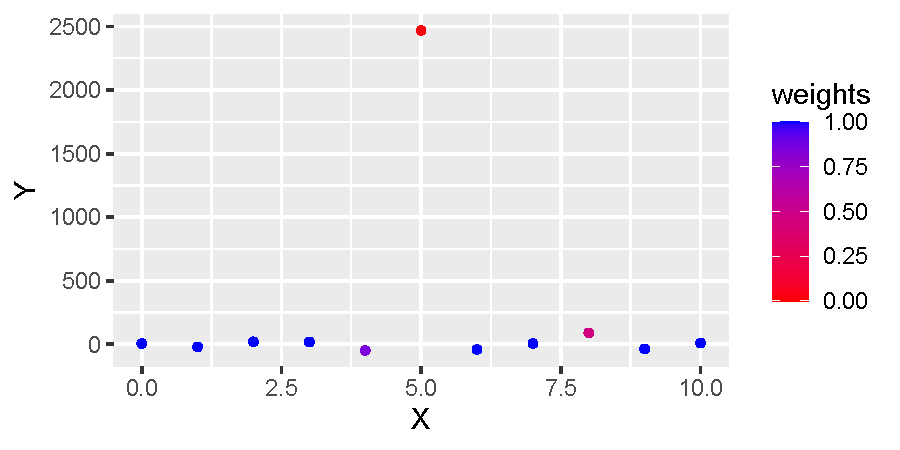
\includegraphics[width=.7\textwidth]{figure/pos-mapping-stage-02-1} 

}


\end{knitrout}

In the second plot we plot the weighted residuals, again with colour for weights. In this case we need to use \ggscale{stage()} to be able to distinguish the mapping ahead of the statistic (\code{start}) from that after the statistic, i.e., ahead of the geometry. We use as above, the default geometry, \gggeom{geom\_point()}. The mapping in this example can be read as: the variable \code{X} from the data frame \code{my.data.outlier} is mapped to the \textit{x} aesthetic at all stages. Variable \code{Y} from the data frame \code{my.data.outlier} is mapped to the \textit{y} aesthetic ahead of the computations in \ggstat{stat\_fit\_residuals()}. After the computations, variables \code{y} and \code{weights} in the data frame returned by \ggstat{stat\_fit\_residuals()} are multiplied and mapped to the \textit{y} ahead of \gggeom{geom\_point()}.\label{chunk:plot:weighted:resid}

\begin{knitrout}\footnotesize
\definecolor{shadecolor}{rgb}{0.969, 0.969, 0.969}\color{fgcolor}\begin{kframe}
\begin{alltt}
\hlkwd{ggplot}\hlstd{(my.data.outlier)} \hlopt{+}
  \hlkwd{stat_fit_residuals}\hlstd{(}\hlkwc{formula} \hlstd{= my.formula,}
                     \hlkwc{method} \hlstd{=} \hlstr{"rlm"}\hlstd{,}
                     \hlkwc{mapping} \hlstd{=} \hlkwd{aes}\hlstd{(}\hlkwc{x} \hlstd{= X,}
                                   \hlkwc{y} \hlstd{=} \hlkwd{stage}\hlstd{(}\hlkwc{start} \hlstd{= Y,}
                                             \hlkwc{after_stat} \hlstd{= y} \hlopt{*} \hlstd{weights),}
                                   \hlkwc{colour} \hlstd{=} \hlkwd{after_stat}\hlstd{(weights)),}
                     \hlkwc{show.legend} \hlstd{=} \hlnum{TRUE}\hlstd{)} \hlopt{+}
  \hlkwd{scale_color_gradient}\hlstd{(}\hlkwc{low} \hlstd{=} \hlstr{"red"}\hlstd{,} \hlkwc{high} \hlstd{=} \hlstr{"blue"}\hlstd{,} \hlkwc{limits} \hlstd{=} \hlkwd{c}\hlstd{(}\hlnum{0}\hlstd{,} \hlnum{1}\hlstd{),}
                       \hlkwc{guide} \hlstd{=} \hlstr{"colourbar"}\hlstd{)}
\end{alltt}
\end{kframe}

{\centering 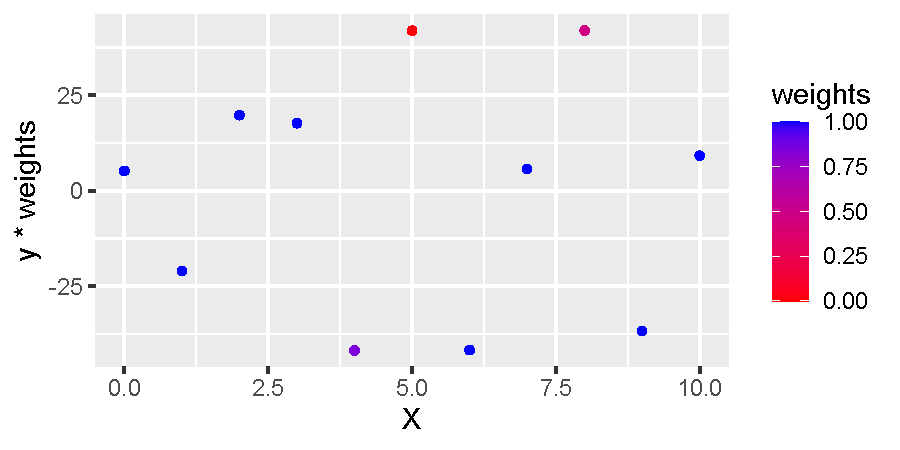
\includegraphics[width=.7\textwidth]{figure/pos-mapping-stage-03-1} 

}


\end{knitrout}

In LM fits, the sum of squares of the un-weighted residuals is minimized to estimate the value of parameters for the best fitting model, while in RLM, the sum of squares of the weighted residuals is minimized instead.

\index{grammar of graphics!mapping of data|)}
\index{grammar of graphics!aesthetics)}

\section{Geometries}\label{sec:plot:geometries}
\index{grammar of graphics!geometries|(}

Different geometries support different \emph{aesthetics}. While \gggeom{geom\_point()} supports \code{shape}, and \gggeom{geom\_line()} supports \code{linetype}, both support \code{x}, \code{y}, \code{color} and \code{size}. In this section we will describe the different \code{geometries} available in package \ggplot and some examples from packages that extend \ggplot. The graphic output from most code examples will not be shown, with the expectation that readers will run them to see the plots.

Mainly for historical reasons, \emph{geometries} accept a \emph{statistic} as an argument, in the same way as \emph{statistics} accept a \emph{geometry} as an argument. In this section we will only describe \emph{geometries} which have as a default \emph{statistic} \code{stat\_identity} which passes values directly as mapped. The \emph{geometries} that have other \emph{statistics} as default are described in section \ref{sec:plot:stat:summaries} together with the corresponding \emph{statistics}.

\subsection{Point}\label{sec:plot:geom:point}
\index{grammar of graphics!point geometry|(}

As shown earlier in this chapter, \gggeom{geom\_point()}, can be used to add a layer with observations represented by ``points'' or symbols. Variable \code{cyl} describes the numbers of cylinders in the engines of the cars. It is a numeric variable, and when mapped to color, a continuous color scale is used to represent this variable.

\index{plots!scatter plot|(}The first examples build scatter plots, because numeric variables are mapped to both \code{x} and \code{y}.
Some scales, like those for \code{color}, exist in two ``flavors,'' one suitable for numeric variables (continuous) and another for factors (discrete).

\begin{knitrout}\footnotesize
\definecolor{shadecolor}{rgb}{0.969, 0.969, 0.969}\color{fgcolor}\begin{kframe}
\begin{alltt}
\hlkwd{ggplot}\hlstd{(}\hlkwc{data} \hlstd{= mtcars,}
       \hlkwd{aes}\hlstd{(}\hlkwc{x} \hlstd{= disp,} \hlkwc{y} \hlstd{= mpg,} \hlkwc{color} \hlstd{= cyl))} \hlopt{+}
  \hlkwd{geom_point}\hlstd{()}
\end{alltt}
\end{kframe}

{\centering 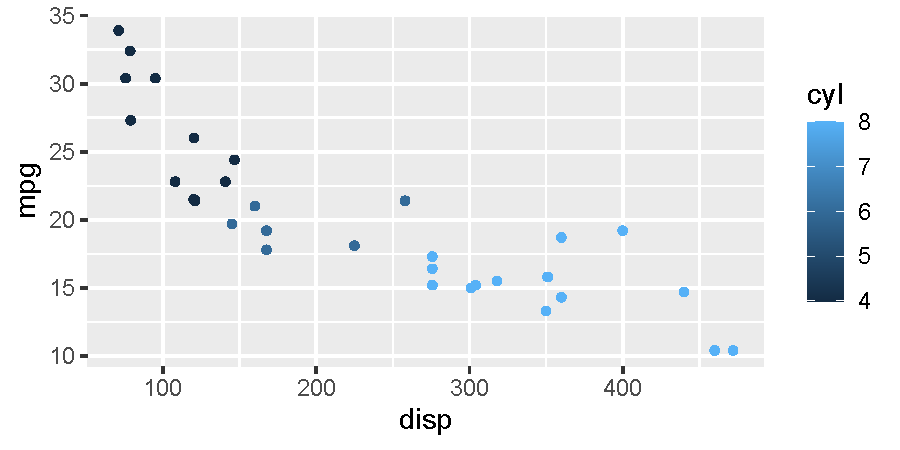
\includegraphics[width=.7\textwidth]{figure/pos-scatter-01-1} 

}


\end{knitrout}

If we convert \code{cyl} into a factor, a discrete color scale is used instead of a continuous one.

\begin{knitrout}\footnotesize
\definecolor{shadecolor}{rgb}{0.969, 0.969, 0.969}\color{fgcolor}\begin{kframe}
\begin{alltt}
\hlkwd{ggplot}\hlstd{(}\hlkwc{data} \hlstd{= mtcars,}
       \hlkwd{aes}\hlstd{(}\hlkwc{x} \hlstd{= disp,} \hlkwc{y} \hlstd{= mpg,} \hlkwc{color} \hlstd{=} \hlkwd{factor}\hlstd{(cyl)))} \hlopt{+}
  \hlkwd{geom_point}\hlstd{()}
\end{alltt}
\end{kframe}
\end{knitrout}

If we convert \code{cyl} into an ordered factor, a different discrete color scale is used by default.

\begin{knitrout}\footnotesize
\definecolor{shadecolor}{rgb}{0.969, 0.969, 0.969}\color{fgcolor}\begin{kframe}
\begin{alltt}
\hlkwd{ggplot}\hlstd{(}\hlkwc{data} \hlstd{= mtcars,}
       \hlkwd{aes}\hlstd{(}\hlkwc{x} \hlstd{= disp,} \hlkwc{y} \hlstd{= mpg,} \hlkwc{color} \hlstd{=} \hlkwd{ordered}\hlstd{(cyl)))} \hlopt{+}
  \hlkwd{geom_point}\hlstd{()}
\end{alltt}
\end{kframe}
\end{knitrout}

\begin{playground}
Try a different mapping: \code{disp} $\rightarrow$ \code{color}, \code{cyl} $\rightarrow$ \code{x}. Continue by using \code{help(mtcars)} and/or \code{names(mtcars)} to see what variables are available, and then try the combinations that trigger your curiosity---i.e., explore the data.
\end{playground}

The mapping between data values and aesthetic values is controlled by scales. Different color scales, and even palettes within a given scale, provide different mappings between data values and rendered colours.

\begin{knitrout}\footnotesize
\definecolor{shadecolor}{rgb}{0.969, 0.969, 0.969}\color{fgcolor}\begin{kframe}
\begin{alltt}
\hlkwd{ggplot}\hlstd{(}\hlkwc{data} \hlstd{= mtcars,}
       \hlkwd{aes}\hlstd{(}\hlkwc{x} \hlstd{= disp,} \hlkwc{y} \hlstd{= mpg,} \hlkwc{color} \hlstd{=} \hlkwd{factor}\hlstd{(cyl)))} \hlopt{+}
  \hlkwd{geom_point}\hlstd{()} \hlopt{+}
  \hlkwd{scale_color_brewer}\hlstd{(}\hlkwc{type} \hlstd{=} \hlstr{"qual"}\hlstd{,} \hlkwc{palette} \hlstd{=} \hlnum{2}\hlstd{)}
\end{alltt}
\end{kframe}
\end{knitrout}

The data, aesthetics mappings, and geometries are the same as in earlier code; to alter how the plot looks, we have changed only the scale and palette used for the color aesthetic. Conceptually it is still exactly the same plot we created earlier, except for the colours used. This is a very important point to understand, because it allows us to separate two different concerns: the semantic structure and the graphic design.

\begin{playground}
Try the different palettes available through the brewer scale. You can play directly with the palettes using function \code{brewer\_pal()} from package \pkgname{scales} together with \code{show\_col()}).

\begin{knitrout}\footnotesize
\definecolor{shadecolor}{rgb}{0.969, 0.969, 0.969}\color{fgcolor}\begin{kframe}
\begin{alltt}
\hlkwd{show_col}\hlstd{(}\hlkwd{brewer_pal}\hlstd{()(}\hlnum{3}\hlstd{))}
\hlkwd{show_col}\hlstd{(}\hlkwd{brewer_pal}\hlstd{(}\hlkwc{type} \hlstd{=} \hlstr{"qual"}\hlstd{,} \hlkwc{palette} \hlstd{=} \hlnum{2}\hlstd{,} \hlkwc{direction} \hlstd{=} \hlnum{1}\hlstd{)(}\hlnum{3}\hlstd{))}
\end{alltt}
\end{kframe}
\end{knitrout}
Once you have found a suitable palette for these data, redo the plot above with the chosen palette.
\end{playground}

When not relying on colors, the most common way of distinguishing groups of observations in scatter plots is to use the \code{shape} of the points as an \emph{aesthetic}. We need to change a single ``word'' in the code statement to achieve this different mapping.

\begin{knitrout}\footnotesize
\definecolor{shadecolor}{rgb}{0.969, 0.969, 0.969}\color{fgcolor}\begin{kframe}
\begin{alltt}
\hlkwd{ggplot}\hlstd{(}\hlkwc{data} \hlstd{= mtcars,} \hlkwd{aes}\hlstd{(}\hlkwc{x} \hlstd{= disp,} \hlkwc{y} \hlstd{= mpg,} \hlkwc{shape} \hlstd{=} \hlkwd{factor}\hlstd{(cyl)))} \hlopt{+}
  \hlkwd{geom_point}\hlstd{()}
\end{alltt}
\end{kframe}
\end{knitrout}

We can use \code{scale\_shape\_manual} to choose each shape to be used. We set three ``open'' shapes that we will see later are very useful as they obey both \code{color} and \code{fill} \emph{aesthetics}.\label{chunk:filled:symbols}

\begin{knitrout}\footnotesize
\definecolor{shadecolor}{rgb}{0.969, 0.969, 0.969}\color{fgcolor}\begin{kframe}
\begin{alltt}
\hlkwd{ggplot}\hlstd{(}\hlkwc{data} \hlstd{= mtcars,} \hlkwd{aes}\hlstd{(}\hlkwc{x} \hlstd{= disp,} \hlkwc{y} \hlstd{= mpg,} \hlkwc{shape} \hlstd{=} \hlkwd{factor}\hlstd{(cyl)))} \hlopt{+}
  \hlkwd{geom_point}\hlstd{()} \hlopt{+}
  \hlkwd{scale_shape_manual}\hlstd{(}\hlkwc{values} \hlstd{=} \hlkwd{c}\hlstd{(}\hlnum{21}\hlstd{,} \hlnum{22}\hlstd{,} \hlnum{23}\hlstd{))}
\end{alltt}
\end{kframe}
\end{knitrout}

It is also possible to use characters as shapes. The character is centered on the position of the observation. As the numbers used as symbols are self-explanatory, we suppress the default guide or key.\label{chunk:plot:point:char}

\begin{knitrout}\footnotesize
\definecolor{shadecolor}{rgb}{0.969, 0.969, 0.969}\color{fgcolor}\begin{kframe}
\begin{alltt}
\hlkwd{ggplot}\hlstd{(}\hlkwc{data} \hlstd{= mtcars,} \hlkwd{aes}\hlstd{(}\hlkwc{x} \hlstd{= disp,} \hlkwc{y} \hlstd{= mpg,} \hlkwc{shape} \hlstd{=} \hlkwd{factor}\hlstd{(cyl)))} \hlopt{+}
  \hlkwd{geom_point}\hlstd{(}\hlkwc{size} \hlstd{=} \hlnum{2.5}\hlstd{)} \hlopt{+}
  \hlkwd{scale_shape_manual}\hlstd{(}\hlkwc{values} \hlstd{=} \hlkwd{c}\hlstd{(}\hlstr{"4"}\hlstd{,} \hlstr{"6"}\hlstd{,} \hlstr{"8"}\hlstd{),} \hlkwc{guide} \hlstd{=} \hlstr{"none"}\hlstd{)}
\end{alltt}
\end{kframe}

{\centering 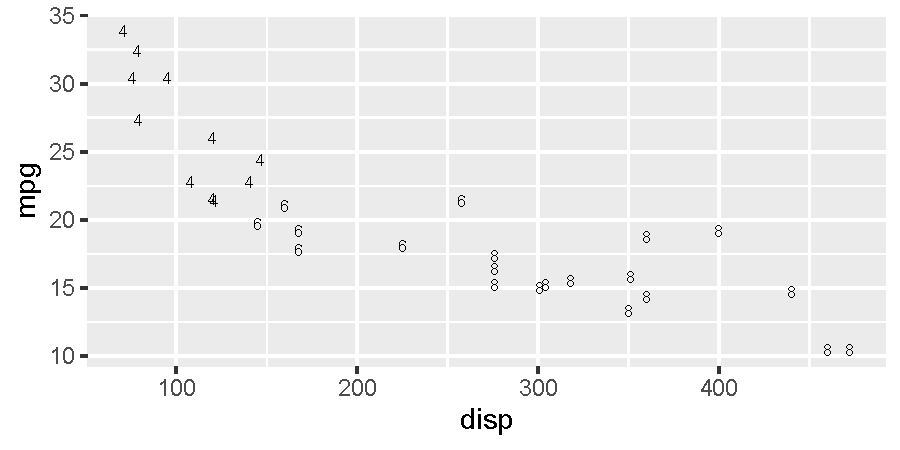
\includegraphics[width=.7\textwidth]{figure/pos-scatter-12-1} 

}


\end{knitrout}

\begin{infobox}
  One variable in the data can be mapped to more than one aesthetic, allowing redundant aesthetics. This may seem wasteful, but it is extremely useful as it allows one to produce figures that, even when produced in color, can still be read if reproduced as black-and-white images.

\begin{knitrout}\footnotesize
\definecolor{shadecolor}{rgb}{0.969, 0.969, 0.969}\color{fgcolor}\begin{kframe}
\begin{alltt}
\hlkwd{ggplot}\hlstd{(}\hlkwc{data} \hlstd{= mtcars,} \hlkwd{aes}\hlstd{(}\hlkwc{x} \hlstd{= disp,} \hlkwc{y} \hlstd{= mpg,}
                          \hlkwc{shape} \hlstd{=} \hlkwd{factor}\hlstd{(cyl),}
                          \hlkwc{color} \hlstd{=} \hlkwd{factor}\hlstd{(cyl)))} \hlopt{+}
  \hlkwd{geom_point}\hlstd{()}
\end{alltt}
\end{kframe}
\end{knitrout}
\end{infobox}

\index{plots!scatter plot|)}
\index{plots!dot plot|(}Dot plots are similar to scatter plots but a factor is mapped to either the \code{x} or \code{y} \emph{aesthetic}. Dot plots are prone to have overlapping observations, and one way of making these points visible is to make them partly transparent by setting a constant value smaller than one for the \code{alpha} \emph{aesthetic}.

\begin{knitrout}\footnotesize
\definecolor{shadecolor}{rgb}{0.969, 0.969, 0.969}\color{fgcolor}\begin{kframe}
\begin{alltt}
\hlkwd{ggplot}\hlstd{(}\hlkwc{data} \hlstd{= mtcars,} \hlkwd{aes}\hlstd{(}\hlkwc{x} \hlstd{=} \hlkwd{factor}\hlstd{(cyl),} \hlkwc{y} \hlstd{= mpg))} \hlopt{+}
  \hlkwd{geom_point}\hlstd{(}\hlkwc{alpha} \hlstd{=} \hlnum{1}\hlopt{/}\hlnum{3}\hlstd{)}
\end{alltt}
\end{kframe}

{\centering 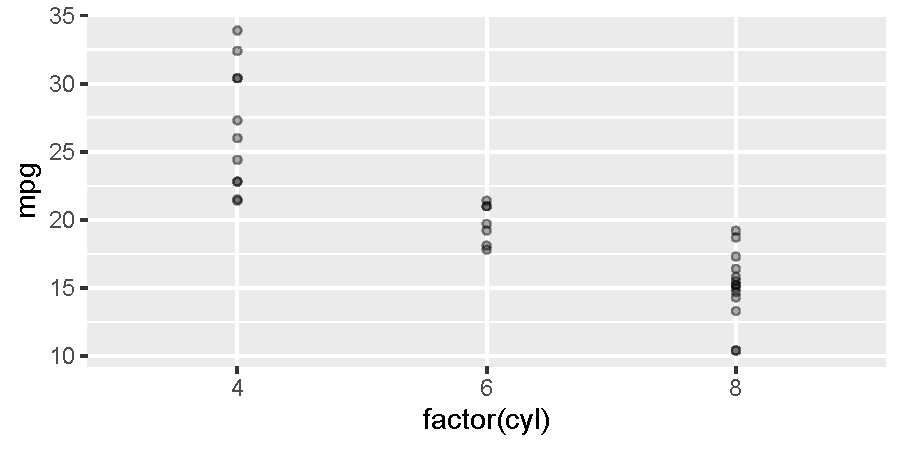
\includegraphics[width=.7\textwidth]{figure/pos-scatter-12a-1} 

}


\end{knitrout}

Instead of making the points semitransparent, we can randomly displace them to avoid overlaps. This is called \emph{jitter}, and can be added using \code{position\_jitter()} and the amount of jitter set with \code{width} as a fraction of the distance between adjacent factor levels in the plot.

\begin{knitrout}\footnotesize
\definecolor{shadecolor}{rgb}{0.969, 0.969, 0.969}\color{fgcolor}\begin{kframe}
\begin{alltt}
\hlkwd{ggplot}\hlstd{(}\hlkwc{data} \hlstd{= mtcars,} \hlkwd{aes}\hlstd{(}\hlkwc{x} \hlstd{=} \hlkwd{factor}\hlstd{(cyl),} \hlkwc{y} \hlstd{= mpg))} \hlopt{+}
  \hlkwd{geom_point}\hlstd{(}\hlkwc{position} \hlstd{=} \hlkwd{position_jitter}\hlstd{(}\hlkwc{width} \hlstd{=} \hlnum{0.05}\hlstd{))}
\end{alltt}
\end{kframe}
\end{knitrout}

\index{plots!dot plot|)}
\index{plots!bubble plot|(}We can create a ``bubble'' plot by mapping the \code{size} \emph{aesthetic} to a continuous variable. In this case, one has to think what is visually more meaningful. Although the radius of the shape is frequently mapped, due to how human perception works, mapping a variable to the area of the shape is more useful by being perceptually closer to a linear mapping. For this example we add a new variable to the plot. The weight of the car in tons and map it to the area of the points.

\begin{knitrout}\footnotesize
\definecolor{shadecolor}{rgb}{0.969, 0.969, 0.969}\color{fgcolor}\begin{kframe}
\begin{alltt}
\hlkwd{ggplot}\hlstd{(}\hlkwc{data} \hlstd{= mtcars,} \hlkwd{aes}\hlstd{(}\hlkwc{x} \hlstd{= disp,} \hlkwc{y} \hlstd{= mpg,}
                          \hlkwc{color} \hlstd{=} \hlkwd{factor}\hlstd{(cyl),}
                          \hlkwc{size} \hlstd{= wt))} \hlopt{+}
  \hlkwd{scale_size_area}\hlstd{()} \hlopt{+}
  \hlkwd{geom_point}\hlstd{()}
\end{alltt}
\end{kframe}

{\centering 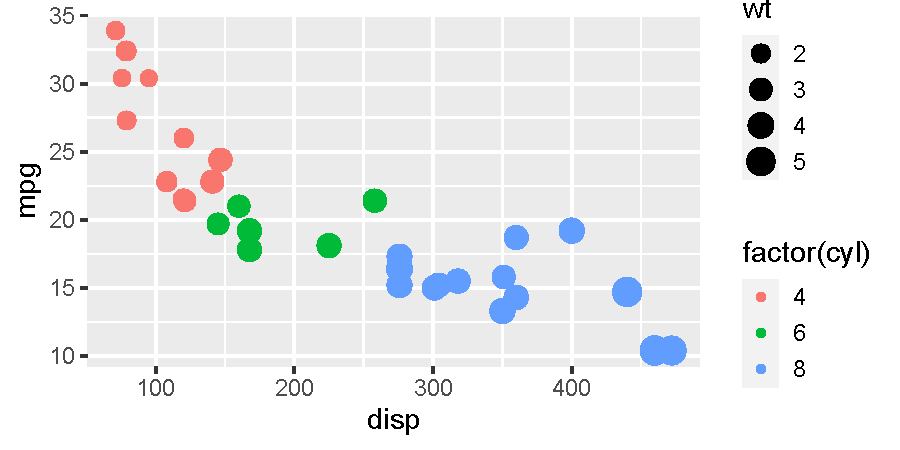
\includegraphics[width=.7\textwidth]{figure/pos-scatter-16-1} 

}


\end{knitrout}

\begin{playground}
If we use a radius-based scale the ``impression'' is different.

\begin{knitrout}\footnotesize
\definecolor{shadecolor}{rgb}{0.969, 0.969, 0.969}\color{fgcolor}\begin{kframe}
\begin{alltt}
\hlkwd{ggplot}\hlstd{(}\hlkwc{data} \hlstd{= mtcars,} \hlkwd{aes}\hlstd{(}\hlkwc{x} \hlstd{= disp,} \hlkwc{y} \hlstd{= mpg,}
                          \hlkwc{color} \hlstd{=} \hlkwd{factor}\hlstd{(cyl),}
                          \hlkwc{size} \hlstd{= wt))} \hlopt{+}
  \hlkwd{scale_size}\hlstd{()} \hlopt{+}
  \hlkwd{geom_point}\hlstd{()}
\end{alltt}
\end{kframe}
\end{knitrout}

Make the plot, look at it carefully. Check the numerical values of some of the weights, and assess if your perception of the plot matches the numbers behind it.
\end{playground}

\index{plots!bubble plot|)}

As a final example summarizing the use of \gggeom{geom\_point()}, we combine different \emph{aesthetics} and \emph{scales} in the same scatter plot.

\begin{knitrout}\footnotesize
\definecolor{shadecolor}{rgb}{0.969, 0.969, 0.969}\color{fgcolor}\begin{kframe}
\begin{alltt}
\hlkwd{ggplot}\hlstd{(}\hlkwc{data} \hlstd{= mtcars,} \hlkwd{aes}\hlstd{(}\hlkwc{x} \hlstd{= disp,} \hlkwc{y} \hlstd{= mpg,}
                          \hlkwc{shape} \hlstd{=} \hlkwd{factor}\hlstd{(cyl),}
                          \hlkwc{fill} \hlstd{=} \hlkwd{factor}\hlstd{(cyl),}
                          \hlkwc{size} \hlstd{= wt))} \hlopt{+}
  \hlkwd{geom_point}\hlstd{(}\hlkwc{alpha} \hlstd{=} \hlnum{0.33}\hlstd{,} \hlkwc{color} \hlstd{=} \hlstr{"black"}\hlstd{)} \hlopt{+}
  \hlkwd{scale_size_area}\hlstd{()} \hlopt{+}
  \hlkwd{scale_shape_manual}\hlstd{(}\hlkwc{values} \hlstd{=} \hlkwd{c}\hlstd{(}\hlnum{21}\hlstd{,} \hlnum{22}\hlstd{,} \hlnum{23}\hlstd{))}
\end{alltt}
\end{kframe}

{\centering 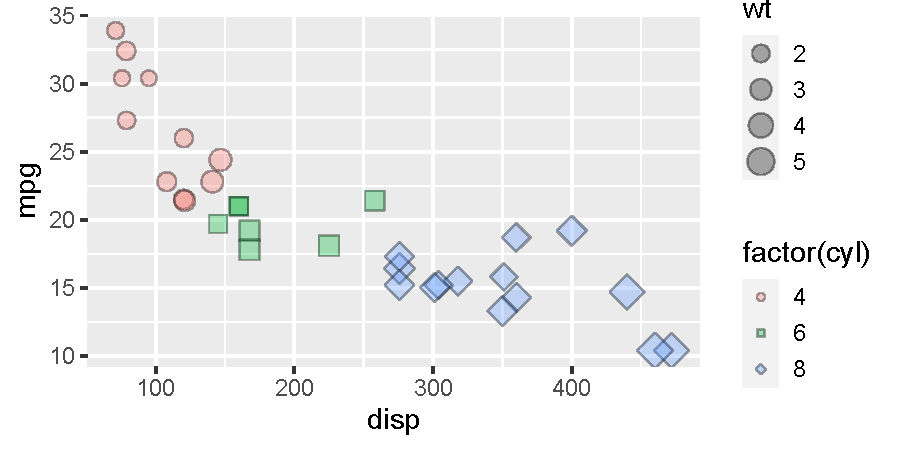
\includegraphics[width=.7\textwidth]{figure/pos-scatter-18-1} 

}


\end{knitrout}

\begin{playground}
Play with the code in the chunk above. Remove or change each of the mappings and the scale, display the new plot, and compare it to the one above. Continue playing with the code until you are sure you understand what graphical element in the plot is added or modified by each individual argument or ``word'' in the code statement.
\end{playground}
\index{grammar of graphics!point geometry|)}

It is common to draw error bars together with points representing means or medians of observations and \gggeom{geom\_pointrange()} achieves this task based on the values mapped to the \code{x}, \code{y}, \code{ymin} and \code{ymax}, using \code{y} for the position of the point and \code{ymin} and \code{ymax} for the positions of the ends of the line segment representing a range. Two other \emph{geometries}, \gggeom{geom\_range()} and  \gggeom{geom\_errorbar()} draw only a segment or a segment with capped ends. They are frequently used together with \emph{statistics} when summaries are calculated on the fly, but can also be used directly when the data summaries are stored in a data frame passed as an argument to \code{data}.

\subsection{Rug}\label{sec:plot:rug}
\index{plots!rug marging|(}

Rarely, rug plots are used by themselves. Instead they are usually an addition to scatter plots. An example of the use of \gggeom{geom\_rug()} follows. They make it easier to see the distribution of observations
along the $x$- and $y$-axes.

\begin{knitrout}\footnotesize
\definecolor{shadecolor}{rgb}{0.969, 0.969, 0.969}\color{fgcolor}\begin{kframe}
\begin{alltt}
\hlkwd{ggplot}\hlstd{(}\hlkwc{data} \hlstd{= mtcars,}
       \hlkwd{aes}\hlstd{(}\hlkwc{x} \hlstd{= disp,} \hlkwc{y} \hlstd{= mpg,} \hlkwc{color} \hlstd{=} \hlkwd{factor}\hlstd{(cyl)))} \hlopt{+}
  \hlkwd{geom_point}\hlstd{()} \hlopt{+}
  \hlkwd{geom_rug}\hlstd{()}
\end{alltt}
\end{kframe}

{\centering 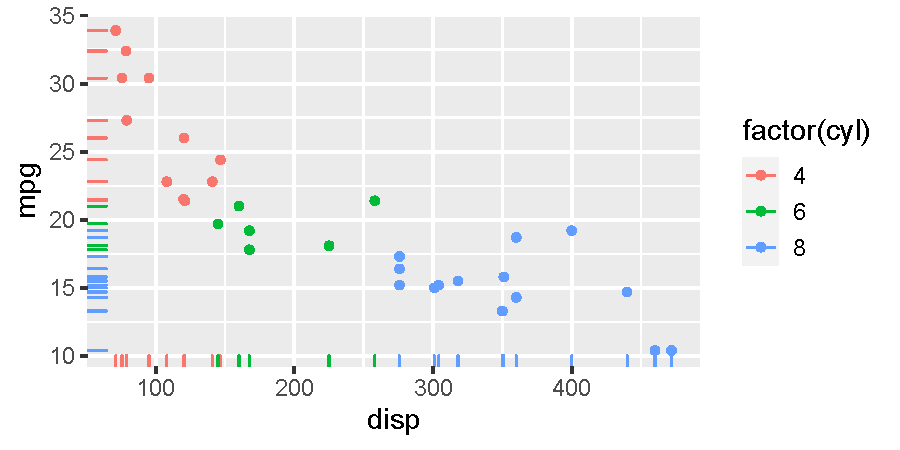
\includegraphics[width=.7\textwidth]{figure/pos-rug-plot-01-1} 

}


\end{knitrout}

\begin{warningbox}
  Rug plots are most useful when the local density of observations is not too high, otherwise rugs become too cluttered and the ``rug threads'' may overlap. When overlap is moderate, making the segments semitransparent by setting the \code{alpha} aesthetic to a constant value smaller than one, can make the variation in density easier to appreciate. When the number of observations is large, marginal density plots should be preferred.
\end{warningbox}
\index{plots!rug marging|)}

\subsection{Line and area}\label{sec:plot:line}

\index{grammar of graphics!various line and path geometries|(}\index{plots!line plot|(}
For line plots we use \gggeom{geom\_line()}. The \code{size} of a line is its thickness, and as we had \code{shape} for points, we have \code{linetype} for lines. In a line plot, observations in successive rows of the data frame, or the subset corresponding to a group, are joined by straight lines. We use a different data set included in \Rlang, \Rdata{Orange}, with data on the growth of five orange trees. See the help page for \code{Orange} for details.

\label{plot:fig:lines}
\begin{knitrout}\footnotesize
\definecolor{shadecolor}{rgb}{0.969, 0.969, 0.969}\color{fgcolor}\begin{kframe}
\begin{alltt}
\hlkwd{ggplot}\hlstd{(}\hlkwc{data} \hlstd{= Orange,}
       \hlkwd{aes}\hlstd{(}\hlkwc{x} \hlstd{= age,} \hlkwc{y} \hlstd{= circumference,} \hlkwc{linetype} \hlstd{= Tree))} \hlopt{+}
  \hlkwd{geom_line}\hlstd{()}
\end{alltt}
\end{kframe}

{\centering 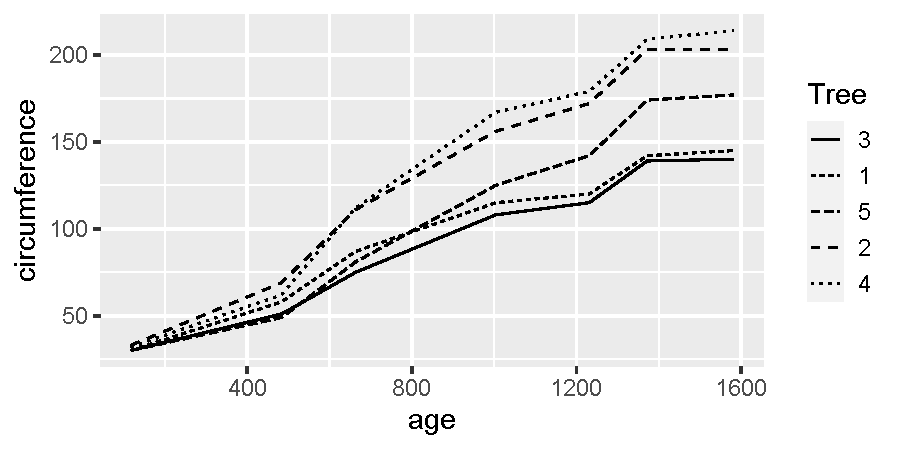
\includegraphics[width=.7\textwidth]{figure/pos-line-plot-01-1} 

}


\end{knitrout}
\index{plots!line plot|)}

\index{plots!step plot|(}
Instead of drawing a line joining the successive observations, we may want to draw a disconnected straight-line segment for each observation or row in the data. In this case, we use \gggeom{geom\_segment()} which accepts \code{x}, \code{xend}, \code{y} and \code{yend} as mapped aesthetics. \gggeom{geom\_curve()} draws curved lines, and the curvature, control points, and angles can be controlled through additional \emph{aesthetics}. These two \emph{geometries} support arrow heads at their ends. Other \emph{geometries} useful for drawing lines or segments are \gggeom{geom\_path()}, which is similar to \gggeom{geom\_line()}, but instead of joining observations according to the values mapped to \code{x}, it joins them according to their row-order in \code{data}, and \gggeom{geom\_spoke()}, which is similar to \gggeom{geom\_segment()} but using a polar parametrization, based on \code{x}, \code{y} for origin, and \code{angle} and \code{radius} for the segment. Finally, \gggeom{geom\_step()} plots only vertical and horizontal lines to join the observations, creating a stepped line.

\begin{knitrout}\footnotesize
\definecolor{shadecolor}{rgb}{0.969, 0.969, 0.969}\color{fgcolor}\begin{kframe}
\begin{alltt}
\hlkwd{ggplot}\hlstd{(}\hlkwc{data} \hlstd{= Orange,}
       \hlkwd{aes}\hlstd{(}\hlkwc{x} \hlstd{= age,} \hlkwc{y} \hlstd{= circumference,} \hlkwc{linetype} \hlstd{= Tree))} \hlopt{+}
  \hlkwd{geom_step}\hlstd{()}
\end{alltt}
\end{kframe}

{\centering 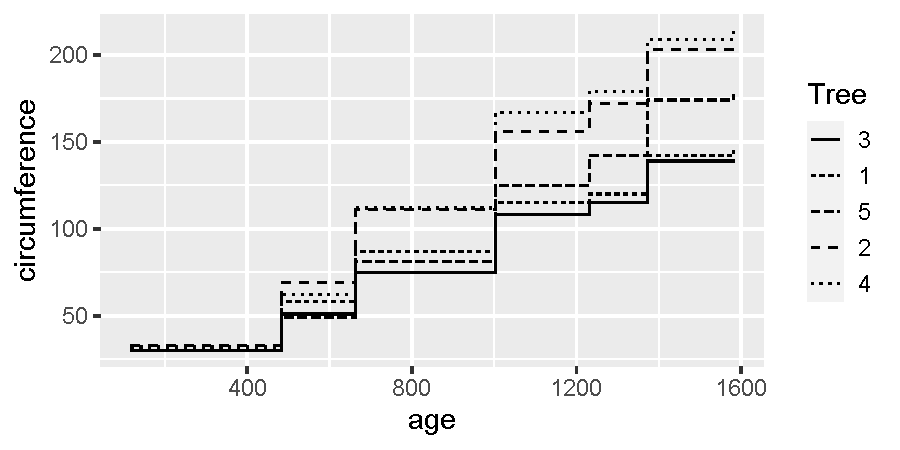
\includegraphics[width=.7\textwidth]{figure/pos-step-plot-01-1} 

}


\end{knitrout}
\index{plots!step plot|)}

\begin{playground}
Using the following toy data, make three plots using \code{geom\_line()}, \code{geom\_path()}, and \code{geom\_step} to add a layer.

\begin{knitrout}\footnotesize
\definecolor{shadecolor}{rgb}{0.969, 0.969, 0.969}\color{fgcolor}\begin{kframe}
\begin{alltt}
\hlstd{toy.df} \hlkwb{<-} \hlkwd{data.frame}\hlstd{(}\hlkwc{x} \hlstd{=} \hlkwd{c}\hlstd{(}\hlnum{1}\hlstd{,}\hlnum{3}\hlstd{,}\hlnum{2}\hlstd{,}\hlnum{4}\hlstd{),} \hlkwc{y} \hlstd{=} \hlkwd{c}\hlstd{(}\hlnum{0}\hlstd{,}\hlnum{1}\hlstd{,}\hlnum{0}\hlstd{,}\hlnum{1}\hlstd{))}
\end{alltt}
\end{kframe}
\end{knitrout}
\end{playground}

\index{plots!filled-area plot|(}
While \gggeom{geom\_line()} draws a line joining observations, \gggeom{geom\_area()} supports filling the area below the line according to the \code{fill} \emph{aesthetic}. In contrast \gggeom{geom\_ribbon()} draws two lines based on the \code{x}, \code{ymin} and \code{ymax} \emph{aesthetics}, with the space between the lines filled according to the \code{fill} \emph{aesthetic}. Finally, \gggeom{geom\_polygon()} is similar to \gggeom{geom\_path()} but connects the extreme observations forming a closed polygon that supports \code{fill}.

Much of what was described above for \gggeom{geom\_point()} can be adapted to \gggeom{geom\_line()}, \gggeom{geom\_ribbon()},  \gggeom{geom\_area()} and other \emph{geometries} described in this section. In some cases, it is useful to stack the areas---e.g.,  when the values represent parts of a bigger whole. In the next, contrived, example, we stack the growth of the different trees by using \code{position = "stack"} instead of the default \code{position = "identity"}. (Compare the $y$ axis of the figure below to that drawn using \code{geom\_line()} on page \pageref{plot:fig:lines}.)

\begin{knitrout}\footnotesize
\definecolor{shadecolor}{rgb}{0.969, 0.969, 0.969}\color{fgcolor}\begin{kframe}
\begin{alltt}
\hlkwd{ggplot}\hlstd{(}\hlkwc{data} \hlstd{= Orange,}
       \hlkwd{aes}\hlstd{(}\hlkwc{x} \hlstd{= age,} \hlkwc{y} \hlstd{= circumference,} \hlkwc{fill} \hlstd{= Tree))} \hlopt{+}
  \hlkwd{geom_area}\hlstd{(}\hlkwc{position} \hlstd{=} \hlstr{"stack"}\hlstd{)}
\end{alltt}
\end{kframe}

{\centering 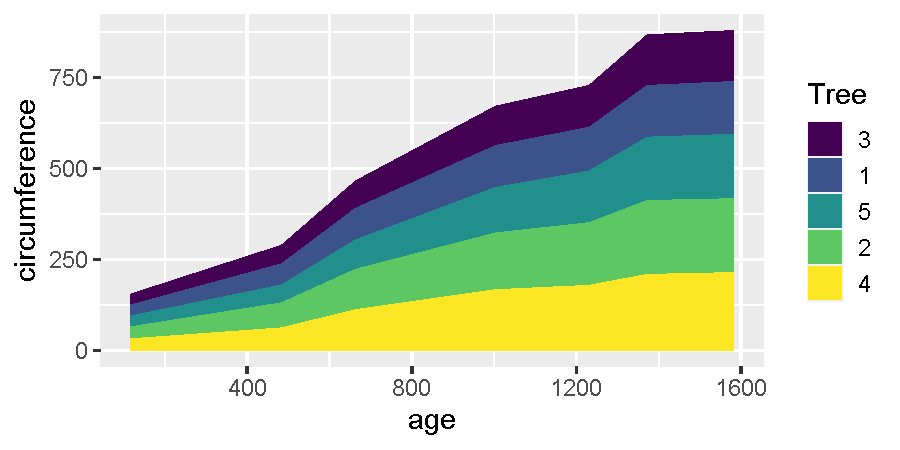
\includegraphics[width=.7\textwidth]{figure/pos-area-plot-01-1} 

}


\end{knitrout}
\index{plots!filled-area plot|)}

\index{plots!reference lines|(}
Finally,\label{sec:plot:vhline} three \emph{geometries} for drawing lines across the whole plotting area: \gggeom{geom\_hline()}, \gggeom{geom\_vline()} and \gggeom{geom\_abline()}. The first two draw horizontal and vertical lines, respectively, while the third one draws straight lines according to the \emph{aesthetics} \code{slope} and \code{intercept} determining the position. The lines drawn with these three geoms extend to the edge of the plotting area.

\gggeom{geom\_hline()} and \gggeom{geom\_vline()} require a single aesthetic, \code{yintercept} and \code{xintercept}, respectively. Different from other geoms, the data for these aesthetics can also be passed as constant numeric vectors. The reason for this is that these geoms are most frequently used to annotate plots rather than plotting observations. Let's assume that we want to highlight an event at the age of 1000 days.

\begin{knitrout}\footnotesize
\definecolor{shadecolor}{rgb}{0.969, 0.969, 0.969}\color{fgcolor}\begin{kframe}
\begin{alltt}
\hlkwd{ggplot}\hlstd{(}\hlkwc{data} \hlstd{= Orange,}
       \hlkwd{aes}\hlstd{(}\hlkwc{x} \hlstd{= age,} \hlkwc{y} \hlstd{= circumference,} \hlkwc{fill} \hlstd{= Tree))} \hlopt{+}
  \hlkwd{geom_area}\hlstd{(}\hlkwc{position} \hlstd{=} \hlstr{"stack"}\hlstd{)} \hlopt{+}
  \hlkwd{geom_vline}\hlstd{(}\hlkwc{xintercept} \hlstd{=} \hlnum{1000}\hlstd{,} \hlkwc{color} \hlstd{=} \hlstr{"gray75"}\hlstd{)} \hlopt{+}
  \hlkwd{geom_vline}\hlstd{(}\hlkwc{xintercept} \hlstd{=} \hlnum{1000}\hlstd{,} \hlkwc{linetype} \hlstd{=} \hlstr{"dotted"}\hlstd{)}
\end{alltt}
\end{kframe}

{\centering 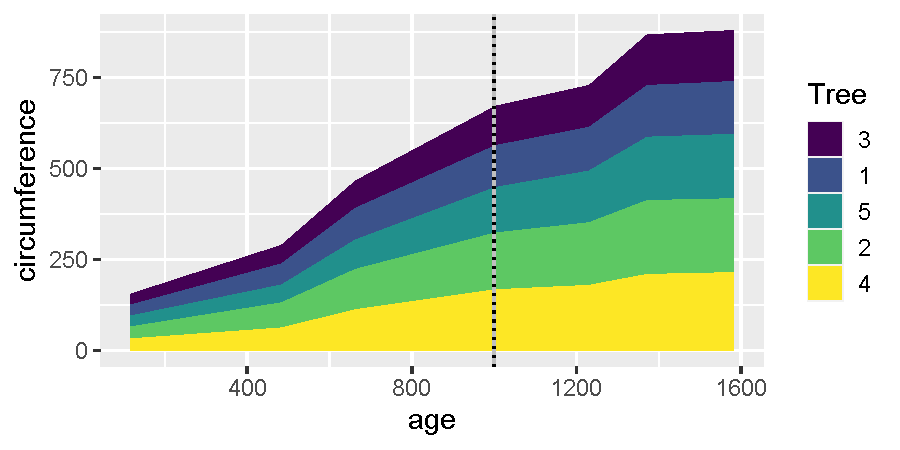
\includegraphics[width=.7\textwidth]{figure/pos-area-plot-02-1} 

}


\end{knitrout}

\begin{playground}
  Change the order of the three layers in the example above. How did the figure change? What order is best? Would the same order be the best for a scatter plot? And would it be necessary to add two \code{geom\_vline()} layers?
\end{playground}
\index{plots!reference lines|)}
\index{grammar of graphics!various line and path geometries|)}

\subsection{Column}\label{sec:plot:col}
\index{grammar of graphics!column geometry|(}
\index{plots!column plot|(}

The \emph{geometry} \gggeom{geom\_col()} can be used to create \emph{column plots} where each bar represents an observation or case in the data.

\begin{warningbox}
\Rlang users not familiar yet with \ggplot are frequently surprised by the default behavior of \gggeom{geom\_bar()} as it uses \ggstat{stat\_count()} to produce a histogram, rather than plotting values as is (see section \ref{sec:plot:histogram} on page \pageref{sec:plot:histogram}). \gggeom{geom\_col()} is identical to \gggeom{geom\_bar()} but with \code{"identity"} as the default statistic.
\end{warningbox}

We create artificial data that we will reuse in multiple variations of the next figure.

\begin{knitrout}\footnotesize
\definecolor{shadecolor}{rgb}{0.969, 0.969, 0.969}\color{fgcolor}\begin{kframe}
\begin{alltt}
\hlkwd{set.seed}\hlstd{(}\hlnum{654321}\hlstd{)}
\hlstd{my.col.data} \hlkwb{<-} \hlkwd{data.frame}\hlstd{(}\hlkwc{treatment} \hlstd{=} \hlkwd{factor}\hlstd{(}\hlkwd{rep}\hlstd{(}\hlkwd{c}\hlstd{(}\hlstr{"A"}\hlstd{,} \hlstr{"B"}\hlstd{,} \hlstr{"C"}\hlstd{),} \hlnum{2}\hlstd{)),}
                          \hlkwc{group} \hlstd{=} \hlkwd{factor}\hlstd{(}\hlkwd{rep}\hlstd{(}\hlkwd{c}\hlstd{(}\hlstr{"male"}\hlstd{,} \hlstr{"female"}\hlstd{),} \hlkwd{c}\hlstd{(}\hlnum{3}\hlstd{,} \hlnum{3}\hlstd{))),}
                          \hlkwc{measurement} \hlstd{=} \hlkwd{rnorm}\hlstd{(}\hlnum{6}\hlstd{)} \hlopt{+} \hlkwd{c}\hlstd{(}\hlnum{5.5}\hlstd{,} \hlnum{5}\hlstd{,} \hlnum{7}\hlstd{))}
\end{alltt}
\end{kframe}
\end{knitrout}

First we plot data for females only, using defaults for all \emph{aesthetics} except $x$ and $y$ which we explicitly map to variables.

\begin{knitrout}\footnotesize
\definecolor{shadecolor}{rgb}{0.969, 0.969, 0.969}\color{fgcolor}\begin{kframe}
\begin{alltt}
\hlkwd{ggplot}\hlstd{(}\hlkwd{subset}\hlstd{(my.col.data, group} \hlopt{==} \hlstr{"female"}\hlstd{),}
       \hlkwd{aes}\hlstd{(}\hlkwc{x} \hlstd{= treatment,} \hlkwc{y} \hlstd{= measurement))} \hlopt{+}
   \hlkwd{geom_col}\hlstd{()}
\end{alltt}
\end{kframe}

{\centering 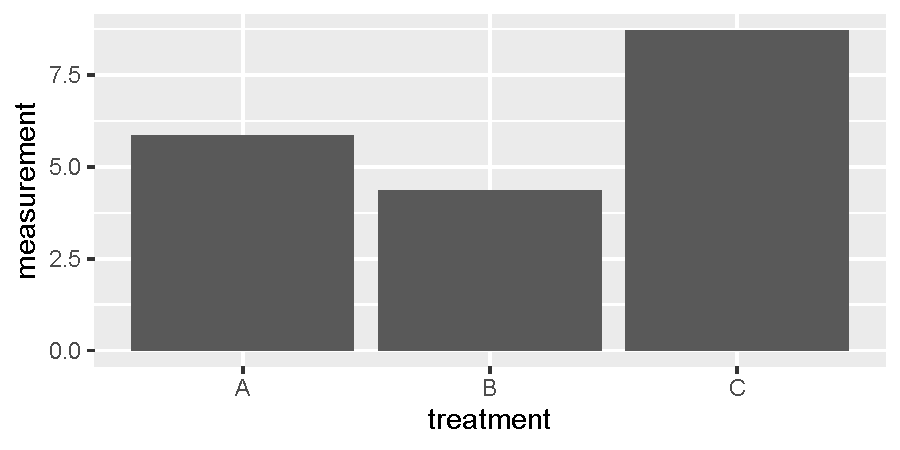
\includegraphics[width=.7\textwidth]{figure/pos-col-plot-02-1} 

}


\end{knitrout}

We play with \emph{aesthetics} to produce a plot with a semi-formal style---e.g.,  suitable for a science popularization article or book. See section \ref{sec:plot:scales} and section \ref{sec:plot:themes} for information on scales and themes, respectively. We set \code{width = 0.5} to make the bars narrower. Setting \code{color = "white"} overrides the default color of the lines bordering the bars.

\begin{knitrout}\footnotesize
\definecolor{shadecolor}{rgb}{0.969, 0.969, 0.969}\color{fgcolor}\begin{kframe}
\begin{alltt}
\hlkwd{ggplot}\hlstd{(my.col.data,} \hlkwd{aes}\hlstd{(}\hlkwc{x} \hlstd{= treatment,} \hlkwc{y} \hlstd{= measurement,} \hlkwc{fill} \hlstd{= group))} \hlopt{+}
     \hlkwd{geom_col}\hlstd{(}\hlkwc{color} \hlstd{=} \hlstr{"white"}\hlstd{,} \hlkwc{width} \hlstd{=} \hlnum{0.5}\hlstd{)} \hlopt{+}
     \hlkwd{scale_fill_grey}\hlstd{()} \hlopt{+} \hlkwd{theme_dark}\hlstd{()}
\end{alltt}
\end{kframe}

{\centering 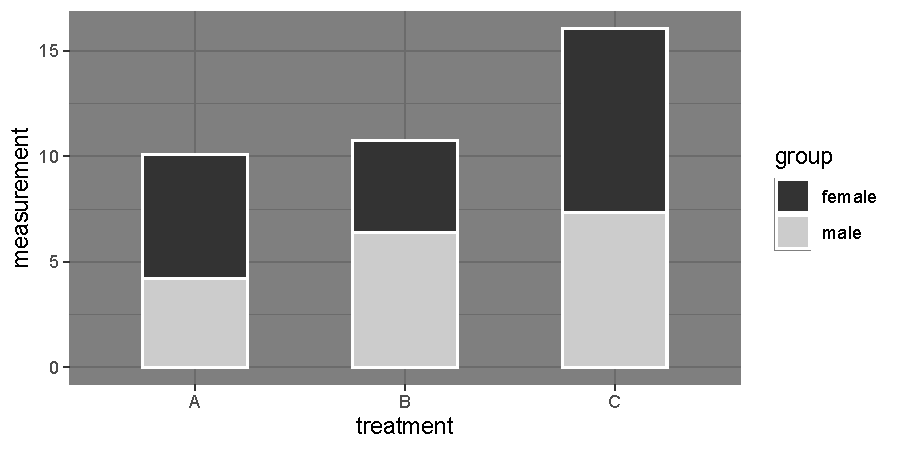
\includegraphics[width=.7\textwidth]{figure/pos-col-plot-03-1} 

}


\end{knitrout}

We next use a formal style, and in addition, put the bars side by side by setting \code{position = "dodge"} to override the default \code{position = "stack"}. Setting \code{color = NA} removes the lines bordering the bars.

\begin{knitrout}\footnotesize
\definecolor{shadecolor}{rgb}{0.969, 0.969, 0.969}\color{fgcolor}\begin{kframe}
\begin{alltt}
\hlkwd{ggplot}\hlstd{(my.col.data,} \hlkwd{aes}\hlstd{(}\hlkwc{x} \hlstd{= treatment,} \hlkwc{y} \hlstd{= measurement,} \hlkwc{fill} \hlstd{= group))} \hlopt{+}
     \hlkwd{geom_col}\hlstd{(}\hlkwc{color} \hlstd{=} \hlnum{NA}\hlstd{,} \hlkwc{position} \hlstd{=} \hlstr{"dodge"}\hlstd{)} \hlopt{+}
     \hlkwd{scale_fill_grey}\hlstd{()} \hlopt{+} \hlkwd{theme_classic}\hlstd{()}
\end{alltt}
\end{kframe}

{\centering 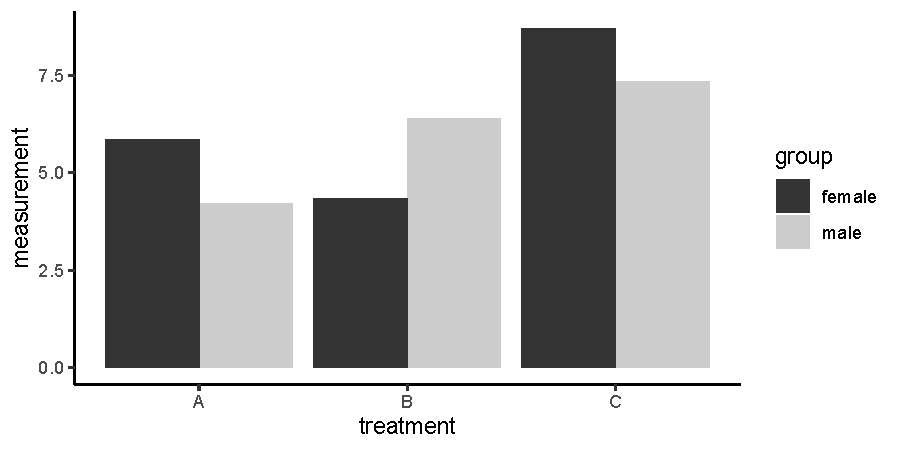
\includegraphics[width=.7\textwidth]{figure/pos-col-plot-04-1} 

}


\end{knitrout}

\begin{playground}
Change the argument to \code{position}, or let the default be active, until you understand its effect on the figure. What is the difference between \emph{positions} \code{"identity"}, \code{"dodge"} and \code{"stack"}?
\end{playground}

\begin{playground}
Use constants as arguments for \emph{aesthetics} or map variable \code{treatment} to one or more of the \emph{aesthetics} used by \gggeom{geom\_col()}, such as \code{color}, \code{fill}, \code{linetype}, \code{size}, \code{alpha} and \code{width}.
\end{playground}

\index{grammar of graphics!column geometry|)}
\index{plots!column plot|)}

\subsection{Tiles}\label{sec:tileplot}
\index{grammar of graphics!tile geometry|(}
\index{plots!tile plot|(}
We can draw square or rectangular tiles with \gggeom{geom\_tile()} producing tile plots or simple heat maps.

We here generate 100 random draws from the $F$ distribution with degrees of freedom $\nu_1 = 5, \nu_2 = 20$.

\begin{knitrout}\footnotesize
\definecolor{shadecolor}{rgb}{0.969, 0.969, 0.969}\color{fgcolor}\begin{kframe}
\begin{alltt}
\hlkwd{set.seed}\hlstd{(}\hlnum{1234}\hlstd{)}
\hlstd{randomf.df} \hlkwb{<-} \hlkwd{data.frame}\hlstd{(}\hlkwc{F.value} \hlstd{=} \hlkwd{rf}\hlstd{(}\hlnum{100}\hlstd{,} \hlkwc{df1} \hlstd{=} \hlnum{5}\hlstd{,} \hlkwc{df2} \hlstd{=} \hlnum{20}\hlstd{),}
                         \hlkwc{x} \hlstd{=} \hlkwd{rep}\hlstd{(letters[}\hlnum{1}\hlopt{:}\hlnum{10}\hlstd{],} \hlnum{10}\hlstd{),}
                         \hlkwc{y} \hlstd{= LETTERS[}\hlkwd{rep}\hlstd{(}\hlnum{1}\hlopt{:}\hlnum{10}\hlstd{,} \hlkwd{rep}\hlstd{(}\hlnum{10}\hlstd{,} \hlnum{10}\hlstd{))])}
\end{alltt}
\end{kframe}
\end{knitrout}

\gggeom{geom\_tile()} requires aesthetics $x$ and $y$, with no defaults, and \code{width} and \code{height} with defaults that make all tiles of equal size filling the plotting area.

\begin{knitrout}\footnotesize
\definecolor{shadecolor}{rgb}{0.969, 0.969, 0.969}\color{fgcolor}\begin{kframe}
\begin{alltt}
\hlkwd{ggplot}\hlstd{(randomf.df,} \hlkwd{aes}\hlstd{(x, y,} \hlkwc{fill} \hlstd{= F.value))} \hlopt{+}
  \hlkwd{geom_tile}\hlstd{()}
\end{alltt}
\end{kframe}

{\centering 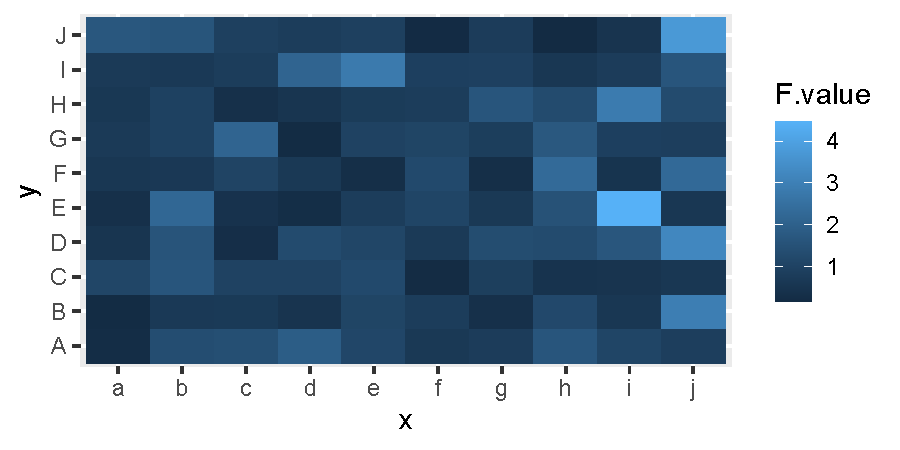
\includegraphics[width=.7\textwidth]{figure/pos-tile-plot-02-1} 

}


\end{knitrout}

We can set \code{color = "gray75"} and \code{size = 1} to make the tile borders more visible as in the example below, or use a contrasting color, to better delineate the borders of the tiles. What to use will depend on whether the individual tiles add meaningful information. In cases like when rows of tiles correspond to individual genes and columns to discrete treatments, the use of contrasting tile borders is preferable. In contrast, in the case when the tiles are an approximation to a continuous surface such as measurements on a regular spatial grid, it is best to suppress the tile borders.

\begin{knitrout}\footnotesize
\definecolor{shadecolor}{rgb}{0.969, 0.969, 0.969}\color{fgcolor}\begin{kframe}
\begin{alltt}
\hlkwd{ggplot}\hlstd{(randomf.df,} \hlkwd{aes}\hlstd{(x, y,} \hlkwc{fill} \hlstd{= F.value))} \hlopt{+}
  \hlkwd{geom_tile}\hlstd{(}\hlkwc{color} \hlstd{=} \hlstr{"gray75"}\hlstd{,} \hlkwc{size} \hlstd{=} \hlnum{1.33}\hlstd{)}
\end{alltt}


{\ttfamily\noindent\color{warningcolor}{\#\# Warning: Using `size` aesthetic for lines was deprecated in ggplot2 3.4.0.\\\#\# i Please use `linewidth` instead.}}\end{kframe}

{\centering 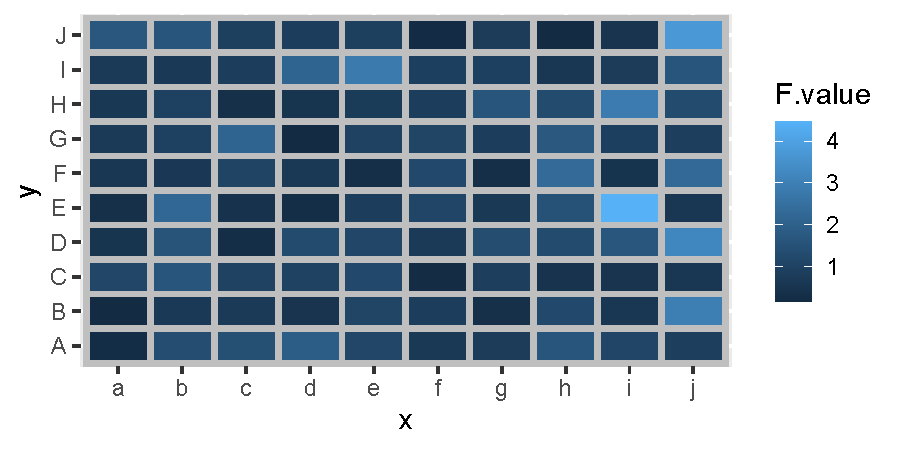
\includegraphics[width=.7\textwidth]{figure/pos-tile-plot-03-1} 

}


\end{knitrout}

\begin{playground}
Play with the arguments passed to parameters \code{color} and \code{size} in the example above, considering what features of the data are most clearly perceived in each of the plots you create.
\end{playground}

Any continuous fill scale can be used to control the appearance. Here we show a tile plot using a gray gradient, with missing values in red.

\begin{knitrout}\footnotesize
\definecolor{shadecolor}{rgb}{0.969, 0.969, 0.969}\color{fgcolor}\begin{kframe}
\begin{alltt}
\hlkwd{ggplot}(randomf.df, \hlkwd{aes}(x, y, fill = F.value) +
  \hlkwd{geom_tile}(color = \hlstr{"white"}) +
  \hlkwd{scale_fill_gradient}(low = \hlstr{"gray15"}, high = \hlstr{"gray85"}, na.value = \hlstr{"red"})
\end{alltt}
\end{kframe}
\end{knitrout}

In contrast to \gggeom{geom\_tile()}, \gggeom{geom\_rect()} draws rectangular tiles based on the position of the corners, mapped to aesthetics \code{xmin}, \code{xmax}, \code{ymin} and \code{ymax}.

\index{plots!tile plot|)}
\index{grammar of graphics!tile geometry|)}

\subsection{Simple features (sf)}\label{sec:plot:sf}
\index{grammar of graphics!sf geometries|(}
\index{plots!maps and spatial plots|(}

\ggplot version 3.0.0 or later supports the plotting of shape data similar to the plotting in geographic information systems (GIS) through \gggeom{geom\_sf()} and its companions, \gggeom{geom\_sf\_text()}, \gggeom{geom\_sf\_label()}, and \ggstat{stat\_sf()}. This makes it possible to display data on maps, for example, using different fill values for different regions. Special \emph{coordinate} \code{coord\_sf()} can be used to select different projections for maps. The \emph{aesthetic} used is called \code{geometry} and contrary to all the other aesthetics we have seen until now, the values to be mapped are of class \code{sfc} containing \emph{simple features} data with multiple components. Manipulation of simple features data is supported by package \pkgname{sf}. This subject exceeds the scope of this book, so a single and very simple example follows.

\begin{knitrout}\footnotesize
\definecolor{shadecolor}{rgb}{0.969, 0.969, 0.969}\color{fgcolor}\begin{kframe}
\begin{alltt}
\hlstd{nc} \hlkwb{<-} \hlstd{sf}\hlopt{::}\hlkwd{st_read}\hlstd{(}\hlkwd{system.file}\hlstd{(}\hlstr{"shape/nc.shp"}\hlstd{,} \hlkwc{package} \hlstd{=} \hlstr{"sf"}\hlstd{),} \hlkwc{quiet} \hlstd{=} \hlnum{TRUE}\hlstd{)}
\hlkwd{ggplot}\hlstd{(nc)} \hlopt{+}
  \hlkwd{geom_sf}\hlstd{(}\hlkwd{aes}\hlstd{(}\hlkwc{fill} \hlstd{= AREA),} \hlkwc{color} \hlstd{=} \hlstr{"gray90"}\hlstd{)}
\end{alltt}
\end{kframe}

{\centering 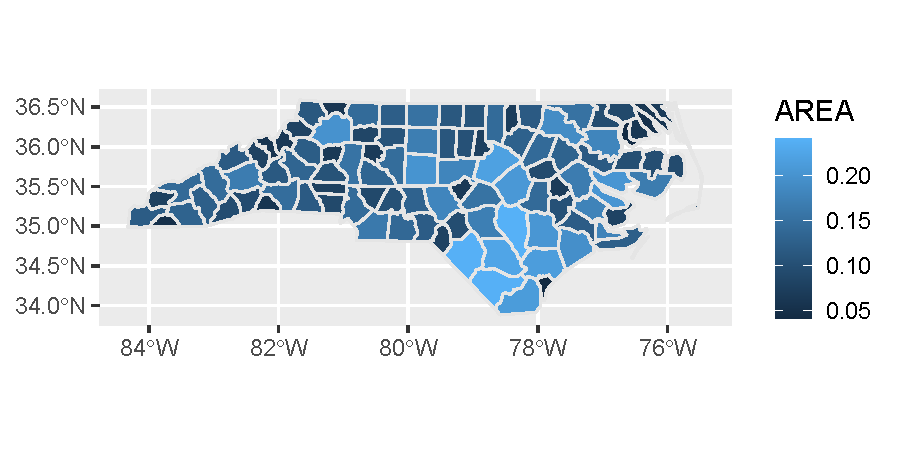
\includegraphics[width=.7\textwidth]{figure/pos-sf_plot-01-1} 

}


\end{knitrout}
\index{grammar of graphics!sf geometries|)}
\index{plots!maps and spatial plots|)}

\subsection{Text}\label{sec:plot:text}
\index{grammar of graphics!text and label geometries|(}
\index{plots!text in|(}
\index{plots!maths in|(}
We can use \gggeom{geom\_text()} or \gggeom{geom\_label()} to add text labels to observations. For \gggeom{geom\_text()} and \gggeom{geom\_label()}, the aesthetic \code{label} provides the text to be plotted and the usual aesthetics \code{x} and \code{y}, the location of the labels. As one would expect, the \code{color} and \code{size} aesthetics can also be used for the text.

\begin{knitrout}\footnotesize
\definecolor{shadecolor}{rgb}{0.969, 0.969, 0.969}\color{fgcolor}\begin{kframe}
\begin{alltt}
\hlkwd{ggplot}\hlstd{(}\hlkwc{data} \hlstd{= mtcars,} \hlkwd{aes}\hlstd{(}\hlkwc{x} \hlstd{= disp,} \hlkwc{y} \hlstd{= mpg,}
                          \hlkwc{color} \hlstd{=} \hlkwd{factor}\hlstd{(cyl),}
                          \hlkwc{size} \hlstd{= wt,}
                          \hlkwc{label} \hlstd{= cyl))} \hlopt{+}
  \hlkwd{scale_size}\hlstd{()} \hlopt{+}
  \hlkwd{geom_point}\hlstd{()} \hlopt{+}
  \hlkwd{geom_text}\hlstd{(}\hlkwc{color} \hlstd{=} \hlstr{"darkblue"}\hlstd{,} \hlkwc{size} \hlstd{=} \hlnum{3}\hlstd{)}
\end{alltt}
\end{kframe}

{\centering 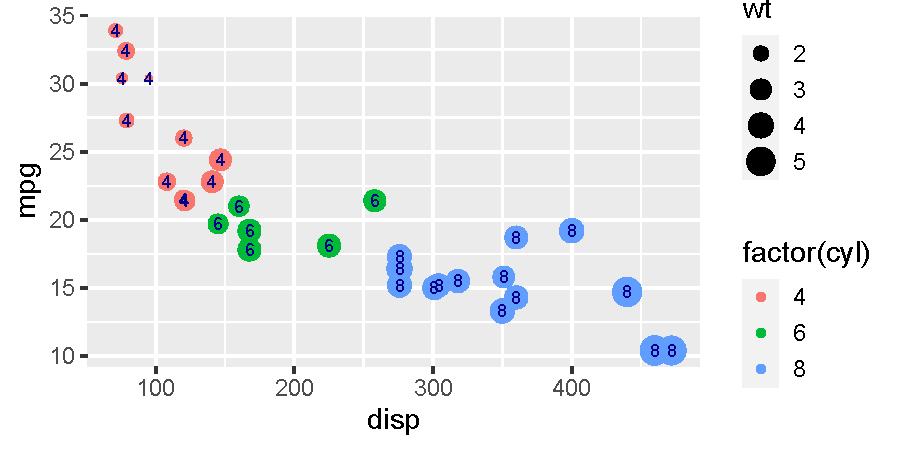
\includegraphics[width=.7\textwidth]{figure/pos-text-plot-01-1} 

}


\end{knitrout}

In addition, \code{angle} and \code{vjust} and \code{hjust} can be used to rotate the text and adjust its position. The default value of 0.5 for both \code{hjust} and \code{vjust} sets the center of the text at the supplied \code{x} and \code{y} coordinates. ``Vertical'' and ``horizontal'' for justification refer to the text, not the plot. This is important when \code{angle} is different from zero. Values larger than 0.5 shift the label left or down, and values smaller than 0.5, right or up with respect to its \code{x} and \code{y} coordinates. A value of 1 or 0 sets the text so that its edge is at the supplied coordinate. Values outside the range $0\ldots 1$ shift the text even farther away, however, still using units based on the length or height of the text label. Recent versions of \pkgname{ggplot2} make possible justification using character constants for alignment: \code{"left"}, \code{"middle"}, \code{"right"}, \code{"bottom"}, \code{"center"} and \code{"top"}, and two special alignments, \code{"inward"} and \code{"outward"}, that automatically vary based on the position in the plotting area.

In the case of \gggeom{geom\_label()} the text is enclosed in a box, which obeys the \code{fill} \emph{aesthetic} and takes additional parameters (described starting at page \pageref{start:plot:label}) allowing control of the shape and size of the box. However, \gggeom{geom\_label()} does not support rotation with the \code{angle} aesthetic.

\begin{warningbox}
You\index{plots!fonts} should be aware that \Rlang and \ggplot support the use of UNICODE\index{UNICODE}, such as UTF8\index{UTF8} character encodings in strings. If your editor or IDE supports their use, then you can type Greek letters and simple maths symbols directly, and they \emph{may} show correctly in labels if a suitable font is loaded and an extended encoding like UTF8 is in use by the operating system. Even if UTF8 is in use, text is not fully portable unless the same font is available\index{portability}, as even if the character positions are standardized for many languages, most UNICODE fonts support at most a small number of languages. In principle one can use this mechanism to have labels both using other alphabets and languages like Chinese with their numerous symbols mixed in the same figure. Furthermore, the support for fonts and consequently character sets in \Rlang is output-device dependent. The font encoding used by \Rlang by default depends on the default locale settings of the operating system, which can also lead to garbage printed to the console or wrong characters being plotted running the same code on a different computer from the one where a script was created. Not all is lost, though, as \Rlang can be coerced to use system fonts and Google fonts with functions provided by packages \pkgname{showtext} and \pkgname{extrafont}. Encoding-related problems, especially in MS-Windows, are common.
\end{warningbox}

In the remaining examples, with output not shown, we use \gggeom{geom\_text()} or \gggeom{geom\_label()} together with \gggeom{geom\_point()} as this is how they may be used to label observations.

\begin{knitrout}\footnotesize
\definecolor{shadecolor}{rgb}{0.969, 0.969, 0.969}\color{fgcolor}\begin{kframe}
\begin{alltt}
\hlstd{my.data} \hlkwb{<-}
  \hlkwd{data.frame}\hlstd{(}\hlkwc{x} \hlstd{=} \hlnum{1}\hlopt{:}\hlnum{5}\hlstd{,}
             \hlkwc{y} \hlstd{=} \hlkwd{rep}\hlstd{(}\hlnum{2}\hlstd{,} \hlnum{5}\hlstd{),}
             \hlkwc{label} \hlstd{=} \hlkwd{c}\hlstd{(}\hlstr{"a"}\hlstd{,} \hlstr{"b"}\hlstd{,} \hlstr{"c"}\hlstd{,} \hlstr{"d"}\hlstd{,} \hlstr{"e"}\hlstd{))}

\hlkwd{ggplot}\hlstd{(my.data,} \hlkwd{aes}\hlstd{(x, y,} \hlkwc{label} \hlstd{= label))} \hlopt{+}
  \hlkwd{geom_text}\hlstd{(}\hlkwc{angle} \hlstd{=} \hlnum{45}\hlstd{,} \hlkwc{hjust} \hlstd{=} \hlnum{1.5}\hlstd{,} \hlkwc{size} \hlstd{=} \hlnum{8}\hlstd{)} \hlopt{+}
  \hlkwd{geom_point}\hlstd{()}
\end{alltt}
\end{kframe}
\end{knitrout}

\begin{playground}
Modify the example above to use \gggeom{geom\_label()} instead of \gggeom{geom\_text()} using, in addition, the \code{fill} aesthetic.
\end{playground}

In the next example we select a different font family, using the same characters in the Roman alphabet. The names \code{"sans"} (the default), \code{"serif"} and \code{"mono"} are recognized by all graphics devices on all operating systems. Additional fonts are available for specific graphic devices, such as the 35 ``PDF'' fonts by the \code{pdf()} device. In this case, their names can be queried with \code{names(pdfFonts())}.

\begin{knitrout}\footnotesize
\definecolor{shadecolor}{rgb}{0.969, 0.969, 0.969}\color{fgcolor}\begin{kframe}
\begin{alltt}
\hlkwd{ggplot}\hlstd{(my.data,} \hlkwd{aes}\hlstd{(x, y,} \hlkwc{label} \hlstd{= label))} \hlopt{+}
  \hlkwd{geom_text}\hlstd{(}\hlkwc{angle} \hlstd{=} \hlnum{45}\hlstd{,} \hlkwc{hjust} \hlstd{=} \hlnum{1.5}\hlstd{,} \hlkwc{size} \hlstd{=} \hlnum{8}\hlstd{,} \hlkwc{family} \hlstd{=} \hlstr{"serif"}\hlstd{)} \hlopt{+}
  \hlkwd{geom_point}\hlstd{()}
\end{alltt}
\end{kframe}
\end{knitrout}

\begin{playground}
In the examples above the character strings were all of the same length, containing a single character. Redo the plots above with longer character strings of various lengths mapped to the \code{label} \emph{aesthetic}. Do also play with justification of these labels.
\end{playground}

Plotting (mathematical) expressions involves mapping to the \code{label} aesthetic character strings that can be parsed as expressions, and setting \code{parse = TRUE} (see section \ref{sec:plot:plotmath} on page \pageref{sec:plot:plotmath}). Here, we build the character strings using \Rfunction{paste()} but, of course, they could also have been entered one by one. This use of \Rfunction{paste()} provides an example of recycling of shorter vectors (see section \ref{sec:vectors} on page \pageref{sec:vectors}).

\begin{knitrout}\footnotesize
\definecolor{shadecolor}{rgb}{0.969, 0.969, 0.969}\color{fgcolor}\begin{kframe}
\begin{alltt}
\hlstd{my.data} \hlkwb{<-}
  \hlkwd{data.frame}\hlstd{(}\hlkwc{x} \hlstd{=} \hlnum{1}\hlopt{:}\hlnum{5}\hlstd{,} \hlkwc{y} \hlstd{=} \hlkwd{rep}\hlstd{(}\hlnum{2}\hlstd{,} \hlnum{5}\hlstd{),} \hlkwc{label} \hlstd{=} \hlkwd{paste}\hlstd{(}\hlstr{"alpha["}\hlstd{,} \hlnum{1}\hlopt{:}\hlnum{5}\hlstd{,} \hlstr{"]"}\hlstd{,} \hlkwc{sep} \hlstd{=} \hlstr{""}\hlstd{))}
\hlstd{my.data}\hlopt{$}\hlstd{label}
\end{alltt}
\begin{verbatim}
## [1] "alpha[1]" "alpha[2]" "alpha[3]" "alpha[4]" "alpha[5]"
\end{verbatim}
\end{kframe}
\end{knitrout}

Text and labels do not automatically expand the plotting area past their anchoring coordinates. In the example above, we need to use \code{expand\_limits()} to ensure that the text is not clipped at the edge of the plotting area.

\begin{knitrout}\footnotesize
\definecolor{shadecolor}{rgb}{0.969, 0.969, 0.969}\color{fgcolor}\begin{kframe}
\begin{alltt}
\hlkwd{ggplot}\hlstd{(my.data,} \hlkwd{aes}\hlstd{(x, y,} \hlkwc{label} \hlstd{= label))} \hlopt{+}
  \hlkwd{geom_text}\hlstd{(}\hlkwc{hjust} \hlstd{=} \hlopt{-}\hlnum{0.2}\hlstd{,} \hlkwc{parse} \hlstd{=} \hlnum{TRUE}\hlstd{,} \hlkwc{size} \hlstd{=} \hlnum{6}\hlstd{)} \hlopt{+}
  \hlkwd{geom_point}\hlstd{()} \hlopt{+}
  \hlkwd{expand_limits}\hlstd{(}\hlkwc{x} \hlstd{=} \hlnum{5.2}\hlstd{)}
\end{alltt}
\end{kframe}

{\centering 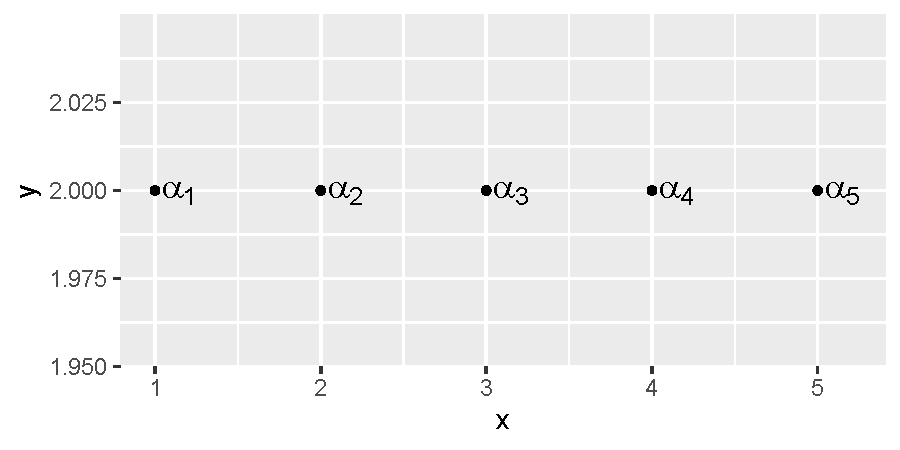
\includegraphics[width=.7\textwidth]{figure/pos-text-plot-06-1} 

}


\end{knitrout}

In the example above, we mapped to label the text to be parsed. It is also possible, and usually preferable, to build suitable labels on the fly within \code{aes()} when setting the mapping for \code{label}. Here we use \gggeom{geom\_text()} with strings to be parsed into expressions created on the fly within the call to \Rfunction{aes()}. The same approach can be used for regular character strings not requiring parsing.

\begin{knitrout}\footnotesize
\definecolor{shadecolor}{rgb}{0.969, 0.969, 0.969}\color{fgcolor}\begin{kframe}
\begin{alltt}
\hlkwd{ggplot}\hlstd{(my.data,} \hlkwd{aes}\hlstd{(x, y,} \hlkwc{label} \hlstd{=} \hlkwd{paste}\hlstd{(}\hlstr{"alpha["}\hlstd{, x,} \hlstr{"]"}\hlstd{,} \hlkwc{sep} \hlstd{=} \hlstr{""}\hlstd{)))} \hlopt{+}
  \hlkwd{geom_text}\hlstd{(}\hlkwc{hjust} \hlstd{=} \hlopt{-}\hlnum{0.2}\hlstd{,} \hlkwc{parse} \hlstd{=} \hlnum{TRUE}\hlstd{,} \hlkwc{size} \hlstd{=} \hlnum{6}\hlstd{)} \hlopt{+}
  \hlkwd{geom_point}\hlstd{()}
\end{alltt}
\end{kframe}
\end{knitrout}

As \gggeom{geom\_label()} obeys the same parameters as \gggeom{geom\_text()} except for \code{angle}, we briefly describe below only the additional parameters compared to \gggeom{geom\_text()}. We may want to alter the default width of the border line or the color used to \code{fill} the rectangle, or to change the ``roundness'' of the corners. To suppress the border line, use \code{label.size = 0}. Corner roundness is controlled by parameter \code{label.r} and the size of the margin around the text by \code{label.padding}.

\label{start:plot:label}
\begin{knitrout}\footnotesize
\definecolor{shadecolor}{rgb}{0.969, 0.969, 0.969}\color{fgcolor}\begin{kframe}
\begin{alltt}
\hlstd{my.data} \hlkwb{<-}
  \hlkwd{data.frame}\hlstd{(}\hlkwc{x} \hlstd{=} \hlnum{1}\hlopt{:}\hlnum{5}\hlstd{,} \hlkwc{y} \hlstd{=} \hlkwd{rep}\hlstd{(}\hlnum{2}\hlstd{,} \hlnum{5}\hlstd{),}
             \hlkwc{label} \hlstd{=} \hlkwd{c}\hlstd{(}\hlstr{"one"}\hlstd{,} \hlstr{"two"}\hlstd{,} \hlstr{"three"}\hlstd{,} \hlstr{"four"}\hlstd{,} \hlstr{"five"}\hlstd{))}

\hlkwd{ggplot}\hlstd{(my.data,} \hlkwd{aes}\hlstd{(x, y,} \hlkwc{label} \hlstd{= label))} \hlopt{+}
  \hlkwd{geom_label}\hlstd{(}\hlkwc{hjust} \hlstd{=} \hlopt{-}\hlnum{0.2}\hlstd{,} \hlkwc{size} \hlstd{=} \hlnum{6}\hlstd{,}
             \hlkwc{label.size} \hlstd{=} \hlnum{0L}\hlstd{,}
             \hlkwc{label.r} \hlstd{=} \hlkwd{unit}\hlstd{(}\hlnum{0}\hlstd{,} \hlstr{"lines"}\hlstd{),}
             \hlkwc{label.padding} \hlstd{=} \hlkwd{unit}\hlstd{(}\hlnum{0.15}\hlstd{,} \hlstr{"lines"}\hlstd{),}
             \hlkwc{fill} \hlstd{=} \hlstr{"yellow"}\hlstd{,} \hlkwc{alpha} \hlstd{=} \hlnum{0.5}\hlstd{)} \hlopt{+}
  \hlkwd{geom_point}\hlstd{()} \hlopt{+}
  \hlkwd{expand_limits}\hlstd{(}\hlkwc{x} \hlstd{=} \hlnum{5.6}\hlstd{)}
\end{alltt}
\end{kframe}

{\centering 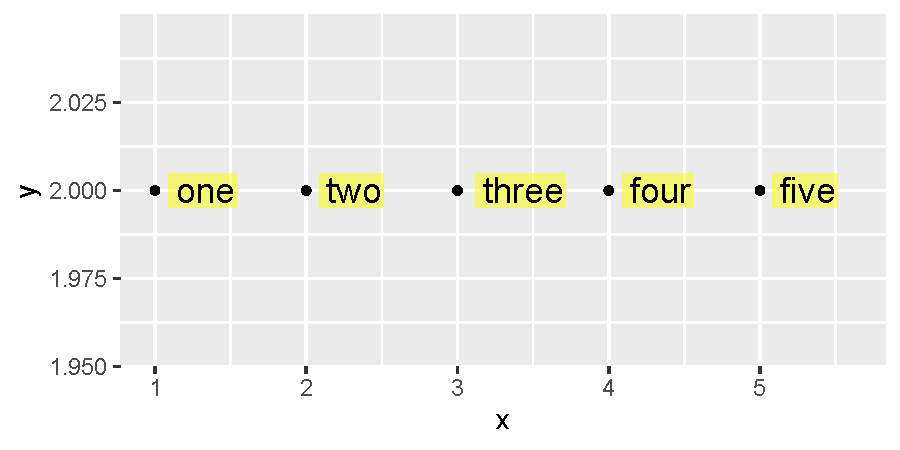
\includegraphics[width=.7\textwidth]{figure/pos-label-plot-01-1} 

}


\end{knitrout}

\begin{playground}
Play with the arguments to the different parameters and with the \emph{aesthetics} to get an idea of what can be done with them. For example, use thicker border lines and increase the padding so that a visually well-balanced margin is retained. You may also try mapping the \code{fill} and \code{color} \emph{aesthetics} to factors in the data.
\end{playground}

If\index{grammar of graphics!text and label geometries!repulsive} the parameter \code{check\_overlap} of \gggeom{geom\_text()} is set to \code{TRUE}, text overlap will be avoided by suppressing the text that would otherwise overlap other text.  \emph{Repulsive} versions of \gggeom{geom\_text()} and \gggeom{geom\_label()}, \gggeom{geom\_text\_repel()} and \gggeom{geom\_label\_repel()},  are available in package \pkgname{ggrepel}. These \emph{geometries} avoid overlaps by automatically repositioning the text or labels. Please read the package documentation for details of how to control the repulsion strength and direction, and the properties of the segments linking the labels to the position of their data coordinates. Nearly all aesthetics supported by \code{geom\_text()} and \code{geom\_label()} are supported by the repulsive versions. However, given that a segment connects the label or text to its anchor point, several properties of these segments can also be controlled with aesthetics or arguments.

\begin{knitrout}\footnotesize
\definecolor{shadecolor}{rgb}{0.969, 0.969, 0.969}\color{fgcolor}\begin{kframe}
\begin{alltt}
\hlkwd{ggplot}\hlstd{(}\hlkwc{data} \hlstd{= mtcars,}
       \hlkwd{aes}\hlstd{(}\hlkwc{x} \hlstd{= disp,} \hlkwc{y} \hlstd{= mpg,} \hlkwc{color} \hlstd{=} \hlkwd{factor}\hlstd{(cyl),} \hlkwc{size} \hlstd{= wt,} \hlkwc{label} \hlstd{= cyl))} \hlopt{+}
  \hlkwd{scale_size}\hlstd{()} \hlopt{+}
  \hlkwd{geom_point}\hlstd{(}\hlkwc{alpha} \hlstd{=} \hlnum{1}\hlopt{/}\hlnum{3}\hlstd{)} \hlopt{+}
  \hlkwd{geom_text_repel}\hlstd{(}\hlkwc{color} \hlstd{=} \hlstr{"black"}\hlstd{,} \hlkwc{size} \hlstd{=} \hlnum{3}\hlstd{,}
                  \hlkwc{min.segment.length} \hlstd{=} \hlnum{0.2}\hlstd{,} \hlkwc{point.padding} \hlstd{=} \hlnum{0.1}\hlstd{)}
\end{alltt}
\end{kframe}

{\centering 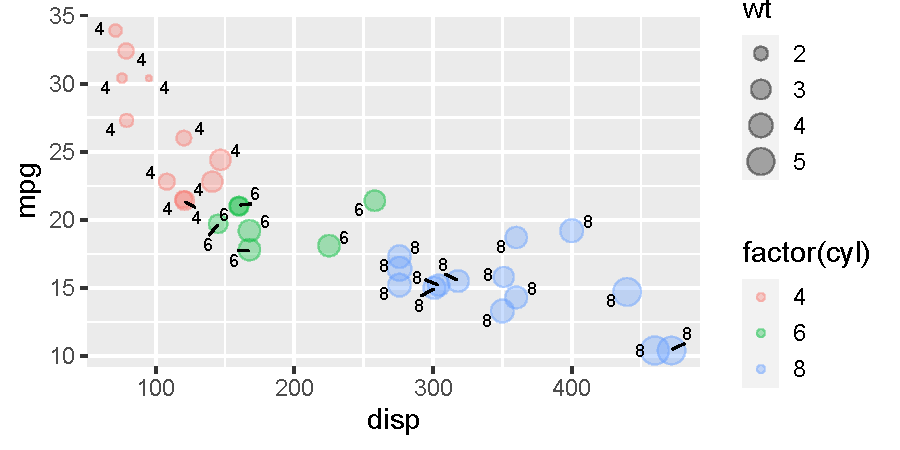
\includegraphics[width=.7\textwidth]{figure/pos-repel-plot-01-1} 

}


\end{knitrout}
\index{plots!maths in|)}
\index{plots!text in|)}
\index{grammar of graphics!text and label geometries|)}

\subsection{Plot insets}\label{sec:plot:insets}
\index{grammar of graphics!inset-related geometries|(}
\index{plots!insets|(}

The support for insets in \pkgname{ggplot2} is confined to \code{annotation\_custom()} which was designed to be used for static annotations expected to be the same in each panel of a plot (the use of annotations is described in section \ref{sec:plot:annotations}). Package \pkgname{ggpmisc} provides geoms that mimic \code{geom\_text()} in relation to the \emph{aesthetics} used, but that similarly to \code{geom\_sf()}, expect that the column in \code{data} mapped to the \code{label} aesthetics are lists of objects containing multiple pieces of information, rather than atomic vectors. Three geometries are currently available: \gggeom{geom\_table()}, \gggeom{geom\_plot()} and \gggeom{geom\_grob()}.

\begin{warningbox}
Given that  \gggeom{geom\_table()}, \gggeom{geom\_plot()} and \gggeom{geom\_grob()} will rarely use a mapping inherited from the whole plot, by default they do not inherit it. Either the mapping should be supplied as an argument to these functions or their parameter \code{inherit.aes} explicitly set to \code{TRUE}.
\end{warningbox}

\index{plots!inset tables|(}
The plotting of tables by mapping a list of data frames to the \code{label} \emph{aesthetic} is done with \gggeom{geom\_table()}. Positioning, justification, and angle work as for \gggeom{geom\_text()} and are applied to the whole table. Only \code{tibble} objects (see documentation of package \pkgname{tibble}) can contain, as variables, lists of data frames, so this \emph{geometry} requires the use of \code{tibble} objects to store the data. The table(s) are created as 'grid' \code{grob} objects, collected in a tree and added to the \code{ggplot} object as a new layer.

We first generate a \code{tibble} containing summaries from the data, formatted as character strings, wrap this tibble in a list, and store this list as a column in another \code{tibble}. To accomplish this, we use functions from the \pkgname{tidyverse} described in chapter \ref{chap:R:data}.

\begin{knitrout}\footnotesize
\definecolor{shadecolor}{rgb}{0.969, 0.969, 0.969}\color{fgcolor}\begin{kframe}
\begin{alltt}
\hlstd{mtcars} \hlopt
  \hlkwd{group_by}\hlstd{(., cyl)} \hlopt
  \hlkwd{summarize}\hlstd{(.,}
            \hlstr{"mean wt"} \hlstd{=} \hlkwd{format}\hlstd{(}\hlkwd{mean}\hlstd{(wt),} \hlkwc{digits} \hlstd{=} \hlnum{3}\hlstd{),}
            \hlstr{"mean disp"} \hlstd{=} \hlkwd{format}\hlstd{(}\hlkwd{mean}\hlstd{(disp),} \hlkwc{digits} \hlstd{=} \hlnum{2}\hlstd{),}
            \hlstr{"mean mpg"} \hlstd{=} \hlkwd{format}\hlstd{(}\hlkwd{mean}\hlstd{(mpg),} \hlkwc{digits} \hlstd{=} \hlnum{2}\hlstd{))} \hlkwb{->} \hlstd{my.table}
\hlstd{table.tb} \hlkwb{<-} \hlkwd{tibble}\hlstd{(}\hlkwc{x} \hlstd{=} \hlnum{500}\hlstd{,} \hlkwc{y} \hlstd{=} \hlnum{35}\hlstd{,} \hlkwc{table.inset} \hlstd{=} \hlkwd{list}\hlstd{(my.table))}
\end{alltt}
\end{kframe}
\end{knitrout}

\begin{knitrout}\footnotesize
\definecolor{shadecolor}{rgb}{0.969, 0.969, 0.969}\color{fgcolor}\begin{kframe}
\begin{alltt}
\hlkwd{ggplot}\hlstd{(}\hlkwc{data} \hlstd{= mtcars,} \hlkwd{aes}\hlstd{(}\hlkwc{x} \hlstd{= disp,} \hlkwc{y} \hlstd{= mpg,}
                          \hlkwc{color} \hlstd{=} \hlkwd{factor}\hlstd{(cyl),}
                          \hlkwc{size} \hlstd{= wt,}
                          \hlkwc{label} \hlstd{= cyl))} \hlopt{+}
  \hlkwd{scale_size}\hlstd{()} \hlopt{+}
  \hlkwd{geom_point}\hlstd{()} \hlopt{+}
  \hlkwd{geom_table}\hlstd{(}\hlkwc{data} \hlstd{= table.tb,}
             \hlkwd{aes}\hlstd{(}\hlkwc{x} \hlstd{= x,} \hlkwc{y} \hlstd{= y,} \hlkwc{label} \hlstd{= table.inset),}
             \hlkwc{color} \hlstd{=} \hlstr{"black"}\hlstd{,} \hlkwc{size} \hlstd{=} \hlnum{3}\hlstd{)}
\end{alltt}
\end{kframe}

{\centering 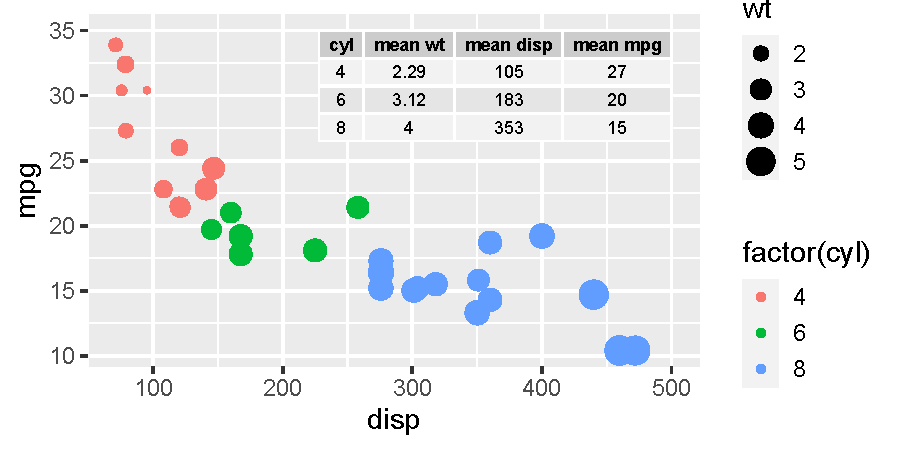
\includegraphics[width=.7\textwidth]{figure/pos-table-plot-02-1} 

}


\end{knitrout}

The \code{color} and \code{size} aesthetics control the text in the table(s) as a whole.
It is also possible to rotate the table(s) using \code{angle}. As with text labels, justification is interpreted in relation to table-text orientation. We set the \code{y = 0} in \code{data.tb} and then use \code{vjust = 1} to position the top of the table at this coordinate value.

\begin{knitrout}\footnotesize
\definecolor{shadecolor}{rgb}{0.969, 0.969, 0.969}\color{fgcolor}\begin{kframe}
\begin{alltt}
\hlkwd{ggplot}\hlstd{(}\hlkwc{data} \hlstd{= mtcars,} \hlkwd{aes}\hlstd{(}\hlkwc{x} \hlstd{= disp,} \hlkwc{y} \hlstd{= mpg,} \hlkwc{color} \hlstd{=} \hlkwd{factor}\hlstd{(cyl)))} \hlopt{+}
  \hlkwd{geom_point}\hlstd{()} \hlopt{+}
  \hlkwd{geom_table}\hlstd{(}\hlkwc{data} \hlstd{= table.tb,}
             \hlkwd{aes}\hlstd{(}\hlkwc{x} \hlstd{= x,} \hlkwc{y} \hlstd{= y,} \hlkwc{label} \hlstd{= table.inset),}
             \hlkwc{color} \hlstd{=} \hlstr{"blue"}\hlstd{,} \hlkwc{size} \hlstd{=} \hlnum{3}\hlstd{,}
             \hlkwc{hjust} \hlstd{=} \hlnum{1}\hlstd{,} \hlkwc{vjust} \hlstd{=} \hlnum{0}\hlstd{,} \hlkwc{angle} \hlstd{=} \hlnum{90}\hlstd{)}
\end{alltt}
\end{kframe}
\end{knitrout}

Parsed text, using R's \emph{plotmath} syntax is supported in the table, with fallback to plain text in case of parsing errors, on a cell-by-cell basis. We end this section with a simple example, which even if not very useful, demonstrates that \gggeom{geom\_table()} behaves like a ``normal'' ggplot \emph{geometry} and that a table can be the only layer in a ggplot if desired. The addition of multiple tables with a single call to \gggeom{geom\_table()} by passing a \code{tibble} with multiple rows as an argument for \code{data} is also possible.

\begin{knitrout}\footnotesize
\definecolor{shadecolor}{rgb}{0.969, 0.969, 0.969}\color{fgcolor}\begin{kframe}
\begin{alltt}
\hlstd{tb.pm} \hlkwb{<-} \hlkwd{tibble}\hlstd{(}\hlstr{'x^0'} \hlstd{=} \hlnum{1}\hlstd{,}
                \hlstr{'x^1'} \hlstd{=} \hlnum{1}\hlopt{:}\hlnum{5}\hlstd{,}
                \hlstr{'x^2'} \hlstd{= (}\hlnum{1}\hlopt{:}\hlnum{5}\hlstd{)}\hlopt{^}\hlnum{2}\hlstd{,}
                \hlstr{'x^3'} \hlstd{= (}\hlnum{1}\hlopt{:}\hlnum{5}\hlstd{)}\hlopt{^}\hlnum{3}\hlstd{)}
\hlstd{data.tb} \hlkwb{<-} \hlkwd{tibble}\hlstd{(}\hlkwc{x} \hlstd{=} \hlnum{1}\hlstd{,} \hlkwc{y} \hlstd{=} \hlnum{1}\hlstd{,} \hlkwc{table.inset} \hlstd{=} \hlkwd{list}\hlstd{(tb.pm))}
\hlkwd{ggplot}\hlstd{(data.tb,} \hlkwc{mapping} \hlstd{=} \hlkwd{aes}\hlstd{(x, y,} \hlkwc{label} \hlstd{= table.inset))} \hlopt{+}
  \hlkwd{geom_table}\hlstd{(}\hlkwc{inherit.aes} \hlstd{=} \hlnum{TRUE}\hlstd{,} \hlkwc{size} \hlstd{=} \hlnum{7}\hlstd{,} \hlkwc{parse} \hlstd{=} \hlnum{TRUE}\hlstd{)} \hlopt{+}
  \hlkwd{theme_void}\hlstd{()}
\end{alltt}
\end{kframe}
\end{knitrout}

\begin{explainbox}
  The \emph{geometry} \gggeom{geom\_table()} uses functions from package \pkgname{gridExtra} to build a graphical object for the table. The use of table themes was not yet supported by this geometry at the time of writing.
\end{explainbox}
\index{plots!inset tables|)}

\index{plots!inset plots|(}
Geometry \gggeom{geom\_plot()} works much like \code{geom\_table()}, but instead of expecting a list of data frames or tibbles to be mapped to the \code{label} aesthetics, it expects a list of ggplots (objects of class \code{gg}). This allows adding as an inset to a ggplot, another ggplot. In the times when plots were hand drafted with India ink on paper, the use of inset plots was more frequent than nowadays. Inset plots can be very useful for zooming-in on parts of a main plot where observations are crowded and for displaying summaries based on the observations shown in the main plot. The inset plots are nested in viewports which control the dimensions of the inset plot, and aesthetics \code{vp.height} and \code{vp.width} control their sizes---with defaults of 1/3 of the height and width of the plotting area of the main plot. Themes can be applied separately to the main and inset plots.

In the first example of inset plots, we include one of the summaries shown above as an inset table. We first create a tibble containing the plot to be inset.

\begin{knitrout}\footnotesize
\definecolor{shadecolor}{rgb}{0.969, 0.969, 0.969}\color{fgcolor}\begin{kframe}
\begin{alltt}
\hlstd{mtcars} \hlopt
  \hlkwd{group_by}\hlstd{(., cyl)} \hlopt
  \hlkwd{summarize}\hlstd{(.,} \hlkwc{mean.mpg} \hlstd{=} \hlkwd{mean}\hlstd{(mpg))} \hlopt
  \hlkwd{ggplot}\hlstd{(}\hlkwc{data} \hlstd{= .,}
         \hlkwd{aes}\hlstd{(}\hlkwd{factor}\hlstd{(cyl), mean.mpg,} \hlkwc{fill} \hlstd{=} \hlkwd{factor}\hlstd{(cyl)))} \hlopt{+}
  \hlkwd{scale_fill_discrete}\hlstd{(}\hlkwc{guide} \hlstd{=} \hlstr{"none"}\hlstd{)} \hlopt{+}
  \hlkwd{scale_y_continuous}\hlstd{(}\hlkwc{name} \hlstd{=} \hlkwa{NULL}\hlstd{)} \hlopt{+}
    \hlkwd{geom_col}\hlstd{()} \hlopt{+}
    \hlkwd{theme_bw}\hlstd{(}\hlnum{8}\hlstd{)} \hlkwb{->} \hlstd{my.plot}
\hlstd{plot.tb} \hlkwb{<-} \hlkwd{tibble}\hlstd{(}\hlkwc{x} \hlstd{=} \hlnum{500}\hlstd{,} \hlkwc{y} \hlstd{=} \hlnum{35}\hlstd{,} \hlkwc{plot.inset} \hlstd{=} \hlkwd{list}\hlstd{(my.plot))}
\end{alltt}
\end{kframe}
\end{knitrout}

\begin{knitrout}\footnotesize
\definecolor{shadecolor}{rgb}{0.969, 0.969, 0.969}\color{fgcolor}\begin{kframe}
\begin{alltt}
\hlkwd{ggplot}\hlstd{(}\hlkwc{data} \hlstd{= mtcars,} \hlkwd{aes}\hlstd{(}\hlkwc{x} \hlstd{= disp,} \hlkwc{y} \hlstd{= mpg,}
                          \hlkwc{color} \hlstd{=} \hlkwd{factor}\hlstd{(cyl)))} \hlopt{+}
  \hlkwd{geom_point}\hlstd{()} \hlopt{+}
  \hlkwd{geom_plot}\hlstd{(}\hlkwc{data} \hlstd{= plot.tb,}
            \hlkwd{aes}\hlstd{(}\hlkwc{x} \hlstd{= x,} \hlkwc{y} \hlstd{= y,} \hlkwc{label} \hlstd{= plot.inset),}
            \hlkwc{vp.width} \hlstd{=} \hlnum{1}\hlopt{/}\hlnum{2}\hlstd{,}
            \hlkwc{hjust} \hlstd{=} \hlstr{"inward"}\hlstd{,} \hlkwc{vjust} \hlstd{=} \hlstr{"inward"}\hlstd{)}
\end{alltt}
\end{kframe}

{\centering 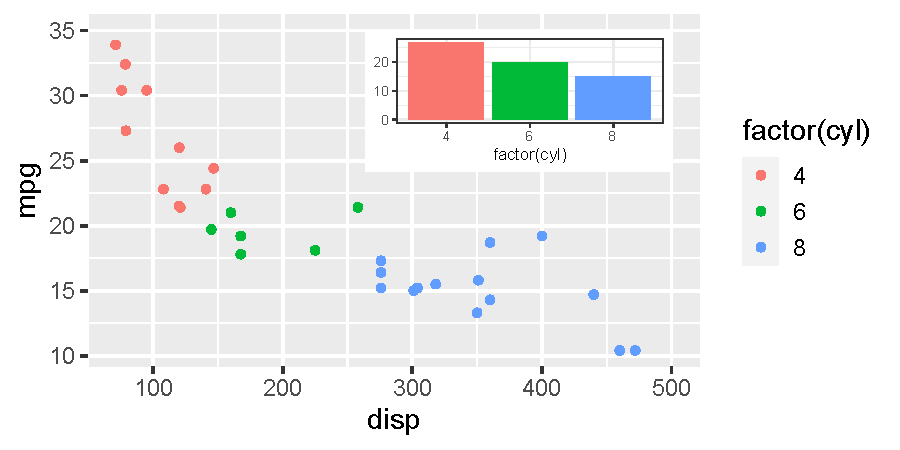
\includegraphics[width=.7\textwidth]{figure/pos-plot-plot-02-1} 

}


\end{knitrout}

In the second example we add the zoomed version of the same plot as an inset. 1) Manually set limits to the coordinates to zoom into a region of the main plot, 2) set the \emph{theme} of the inset, 3) remove axis labels as they are the same as in the main plot, 4) and 5) highlight the zoomed-in region in the main plot. This fairly complex example shows how a new extension to \pkgname{ggplot2} can integrate well into the grammar of graphics paradigm. In this example, to show an alternative approach, instead of collecting all the data into a data frame, we map constant values directly to the various aesthetics within \Rfunction{annotate()} (see section \ref{sec:plot:annotations} on page \pageref{sec:plot:annotations}).

\begin{knitrout}\footnotesize
\definecolor{shadecolor}{rgb}{0.969, 0.969, 0.969}\color{fgcolor}\begin{kframe}
\begin{alltt}
\hlstd{p.main} \hlkwb{<-} \hlkwd{ggplot}\hlstd{(}\hlkwc{data} \hlstd{= mtcars,} \hlkwd{aes}\hlstd{(}\hlkwc{x} \hlstd{= disp,} \hlkwc{y} \hlstd{= mpg,} \hlkwc{color} \hlstd{=} \hlkwd{factor}\hlstd{(cyl)))} \hlopt{+}
  \hlkwd{geom_point}\hlstd{()}
\hlstd{p.inset} \hlkwb{<-} \hlstd{p.main} \hlopt{+}
  \hlkwd{coord_cartesian}\hlstd{(}\hlkwc{xlim} \hlstd{=} \hlkwd{c}\hlstd{(}\hlnum{270}\hlstd{,} \hlnum{330}\hlstd{),} \hlkwc{ylim} \hlstd{=} \hlkwd{c}\hlstd{(}\hlnum{14}\hlstd{,} \hlnum{19}\hlstd{))} \hlopt{+}
  \hlkwd{labs}\hlstd{(}\hlkwc{x} \hlstd{=} \hlkwa{NULL}\hlstd{,} \hlkwc{y} \hlstd{=} \hlkwa{NULL}\hlstd{)} \hlopt{+}
  \hlkwd{scale_color_discrete}\hlstd{(}\hlkwc{guide} \hlstd{=} \hlstr{"none"}\hlstd{)} \hlopt{+}
  \hlkwd{theme_bw}\hlstd{(}\hlnum{8}\hlstd{)} \hlopt{+} \hlkwd{theme}\hlstd{(}\hlkwc{aspect.ratio} \hlstd{=} \hlnum{1}\hlstd{)}
\hlstd{p.main} \hlopt{+}
  \hlkwd{geom_plot}\hlstd{(}\hlkwc{x} \hlstd{=} \hlnum{480}\hlstd{,} \hlkwc{y} \hlstd{=} \hlnum{34}\hlstd{,} \hlkwc{label} \hlstd{=} \hlkwd{list}\hlstd{(p.inset),} \hlkwc{vp.height} \hlstd{=} \hlnum{1}\hlopt{/}\hlnum{2}\hlstd{,}
            \hlkwc{hjust} \hlstd{=} \hlstr{"inward"}\hlstd{,} \hlkwc{vjust} \hlstd{=} \hlstr{"inward"}\hlstd{)} \hlopt{+}
  \hlkwd{annotate}\hlstd{(}\hlkwc{geom} \hlstd{=} \hlstr{"rect"}\hlstd{,} \hlkwc{fill} \hlstd{=} \hlnum{NA}\hlstd{,} \hlkwc{color} \hlstd{=} \hlstr{"black"}\hlstd{,}
           \hlkwc{xmin} \hlstd{=} \hlnum{270}\hlstd{,} \hlkwc{xmax} \hlstd{=} \hlnum{330}\hlstd{,} \hlkwc{ymin} \hlstd{=} \hlnum{14}\hlstd{,} \hlkwc{ymax} \hlstd{=} \hlnum{19}\hlstd{,}
           \hlkwc{linetype} \hlstd{=} \hlstr{"dotted"}\hlstd{)}
\end{alltt}
\end{kframe}

{\centering 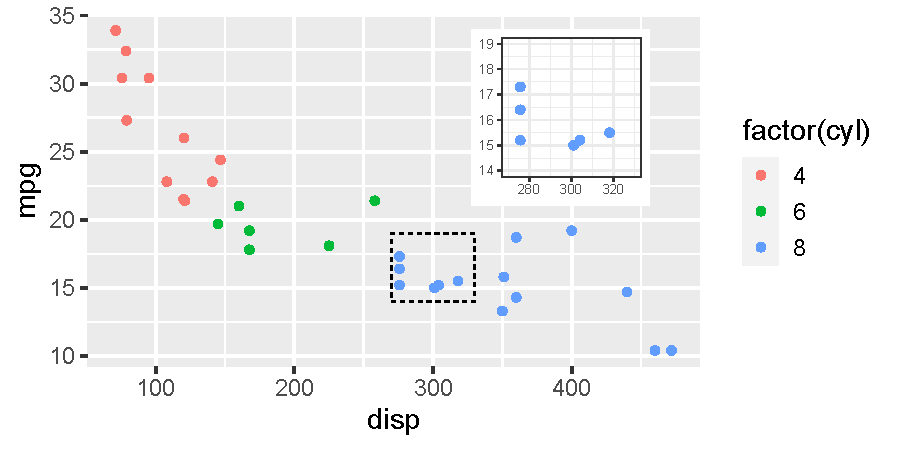
\includegraphics[width=.7\textwidth]{figure/pos-plot-plot-03-1} 

}


\end{knitrout}
\index{plots!inset plots|)}
\index{plots!inset graphical objects|(}
Geometry \gggeom{geom\_grob()} works much like \code{geom\_table()} and \code{geom\_plot()} but expects a list of \pkgname{grid} graphical objects, called \code{grob} for short. This adds generality at the expense of having to separately create the grobs either using \pkgname{grid} or by converting other objects into grobs. This geometry is as flexible as \gggeom{annotation\_custom()} with respect to the grobs, but behaves as a \emph{geometry}. We show an example that adds two bitmaps to the plot. The bitmaps are read from PNG files, converted into grobs, and added to the plot as a new layer. The PNG bitmaps used have a transparent background.

\begin{knitrout}\footnotesize
\definecolor{shadecolor}{rgb}{0.969, 0.969, 0.969}\color{fgcolor}\begin{kframe}
\begin{alltt}
\hlstd{file1.name} \hlkwb{<-}
  \hlkwd{system.file}\hlstd{(}\hlstr{"extdata"}\hlstd{,} \hlstr{"Isoquercitin.png"}\hlstd{,} \hlkwc{package} \hlstd{=} \hlstr{"ggpmisc"}\hlstd{,} \hlkwc{mustWork} \hlstd{=} \hlnum{TRUE}\hlstd{)}
\hlstd{Isoquercitin} \hlkwb{<-} \hlstd{magick}\hlopt{::}\hlkwd{image_read}\hlstd{(file1.name)}
\hlstd{file2.name} \hlkwb{<-}
  \hlkwd{system.file}\hlstd{(}\hlstr{"extdata"}\hlstd{,} \hlstr{"Robinin.png"}\hlstd{,} \hlkwc{package} \hlstd{=} \hlstr{"ggpmisc"}\hlstd{,} \hlkwc{mustWork} \hlstd{=} \hlnum{TRUE}\hlstd{)}
\hlstd{Robinin} \hlkwb{<-} \hlstd{magick}\hlopt{::}\hlkwd{image_read}\hlstd{(file2.name)}
\hlstd{grob.tb} \hlkwb{<-} \hlkwd{tibble}\hlstd{(}\hlkwc{x} \hlstd{=} \hlkwd{c}\hlstd{(}\hlnum{0}\hlstd{,} \hlnum{100}\hlstd{),} \hlkwc{y} \hlstd{=} \hlkwd{c}\hlstd{(}\hlnum{10}\hlstd{,} \hlnum{20}\hlstd{),} \hlkwc{height} \hlstd{=} \hlnum{1}\hlopt{/}\hlnum{3}\hlstd{,} \hlkwc{width} \hlstd{=} \hlkwd{c}\hlstd{(}\hlnum{1}\hlopt{/}\hlnum{2}\hlstd{),}
                  \hlkwc{grobs} \hlstd{=} \hlkwd{list}\hlstd{(grid}\hlopt{::}\hlkwd{rasterGrob}\hlstd{(}\hlkwc{image} \hlstd{= Isoquercitin),}
                               \hlstd{grid}\hlopt{::}\hlkwd{rasterGrob}\hlstd{(}\hlkwc{image} \hlstd{= Robinin)))}

\hlkwd{ggplot}\hlstd{()} \hlopt{+}
  \hlkwd{geom_grob}\hlstd{(}\hlkwc{data} \hlstd{= grob.tb,}
            \hlkwd{aes}\hlstd{(}\hlkwc{x} \hlstd{= x,} \hlkwc{y} \hlstd{= y,} \hlkwc{label} \hlstd{= grobs,} \hlkwc{vp.height} \hlstd{= height,} \hlkwc{vp.width} \hlstd{= width),}
                \hlkwc{hjust} \hlstd{=} \hlstr{"inward"}\hlstd{,} \hlkwc{vjust} \hlstd{=} \hlstr{"inward"}\hlstd{)}
\end{alltt}
\end{kframe}

{\centering 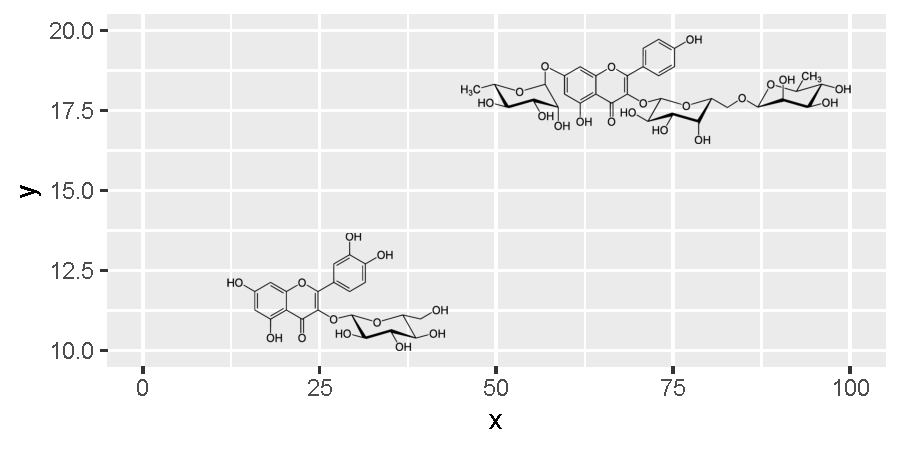
\includegraphics[width=.7\textwidth]{figure/pos-plot-grob-01-1} 

}


\end{knitrout}
\index{plots!inset graphical objects|)}

\begin{explainbox}
Grid graphics\index{grid graphics coordinate systems} provide the low-level functions that both \pkgname{ggplot2} and \pkgname{lattice} use under the hood. Grid supports different types of units for expressing the coordinates of positions within the plotting area. All examples outside this text box use \code{"native"} data coordinates, however, coordinates can be also given in physical units like \code{"mm"}. More useful when working with scalable plots is to use "npc" \emph{normalized parent coordinates}, which are expressed as numbers in the range 0 to 1, relative to the dimensions of the sides of the current \emph{viewport}, with origin at the lower left corner.

Package \pkgname{ggplot2} interprets $x$ and $y$ coordinates in \code{"native"} data coordinates, and trickery seems to be needed to get around this limitation. A rather general solution is provided by package \pkgname{ggpmisc} through \emph{aesthetics} \code{npcx} and \code{npcy} and \emph{geometries} that support them. At the time of writing, \gggeom{geom\_text\_npc()}, \gggeom{geom\_label\_npc()}, \gggeom{geom\_table\_npc()}, \gggeom{geom\_plot\_npc()} and \gggeom{geom\_grob\_npc()}. These \emph{geometries} are useful for annotating plots and adding insets at positions relative to the plotting area that remain always consistent across different plots, or across panels when using facets with free axis limits. Being geometries they provide freedom in the elements added to different panels and their positions.

\begin{knitrout}\footnotesize
\definecolor{shadecolor}{rgb}{0.969, 0.969, 0.969}\color{fgcolor}\begin{kframe}
\begin{alltt}
\hlkwd{ggplot}\hlstd{(}\hlkwc{data} \hlstd{= mtcars,} \hlkwd{aes}\hlstd{(}\hlkwc{x} \hlstd{= disp,} \hlkwc{y} \hlstd{= mpg,} \hlkwc{color} \hlstd{=} \hlkwd{factor}\hlstd{(cyl)))} \hlopt{+}
  \hlkwd{geom_point}\hlstd{()} \hlopt{+}
  \hlkwd{geom_label_npc}\hlstd{(}\hlkwc{npcx} \hlstd{=} \hlnum{0.5}\hlstd{,} \hlkwc{npcy} \hlstd{=} \hlnum{0.9}\hlstd{,} \hlkwc{label} \hlstd{=} \hlstr{"a label"}\hlstd{,} \hlkwc{color} \hlstd{=} \hlstr{"black"}\hlstd{)}
\end{alltt}
\end{kframe}

{\centering 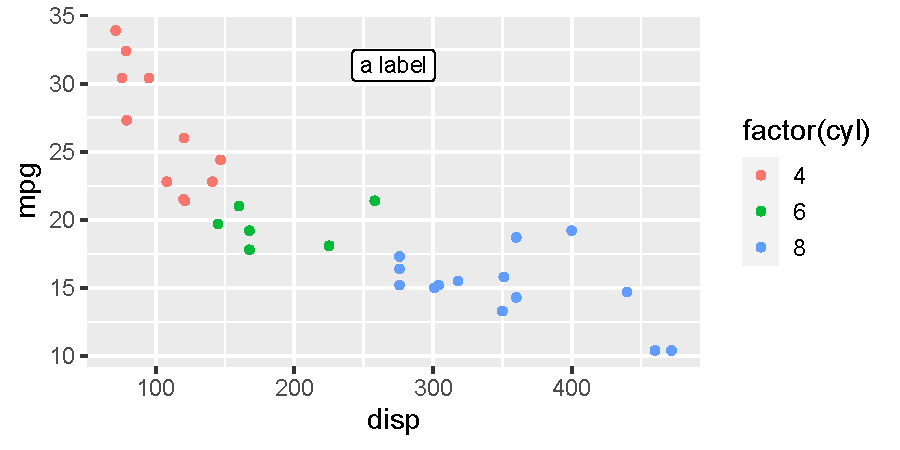
\includegraphics[width=.7\textwidth]{figure/pos-plot-npc-eb-01-1} 

}


\end{knitrout}

\end{explainbox}

\index{grammar of graphics!inset-related geometries|)}
\index{plots!insets|)}
\index{grammar of graphics!geometries|)}

\section{Statistics}\label{sec:plot:statistics}
\index{grammar of graphics!statistics|(}

Before learning about \ggplot \emph{statistics}, it is important to have clear how the mapping of factors to \emph{aesthetics} works. When a factor, for example, is mapped to \code{color}, it creates a new grouping, with the observations matching a given level of the factor, corresponding to a group. Most \emph{statistics} operate on the data for each of these groups separately, returning a summary for each group, for example, the mean of the observations in a group.

\subsection{Functions}\label{sec:plot:function}
\index{grammar of graphics!function statistic|(}
\index{plots!plots of functions|(}
In addition to plotting data from a data frame with variables to map to $x$ and $y$ \emph{aesthetics}, it is possible to have only a variable mapped to $x$ and use \ggstat{stat\_function()} to compute the values to be mapped to $y$ using an \Rlang function. This avoids the need to generate data beforehand as even the number of data points to be generated can be set in \code{geom\_function()}. Any \Rlang function, user defined or not, can be used as long as it is vectorized, with the length of the returned vector equal to the length of the vector passed as first argument to it. The variable mapped to \code{x} determines the range, and the argument to parameter \code{n} of \code{geom\_function()} the length of the generated vector that is passed as first argument to \code{fun} when it is called to generate the values to napped to \code{y}. These are the $x$ and $y$ values passed to the \emph{geometry}.

We start with the Normal distribution function. We rely on the defaults \code{n = 101} and \code{geom = "path"}.

\begin{knitrout}\footnotesize
\definecolor{shadecolor}{rgb}{0.969, 0.969, 0.969}\color{fgcolor}\begin{kframe}
\begin{alltt}
\hlkwd{ggplot}\hlstd{(}\hlkwd{data.frame}\hlstd{(}\hlkwc{x} \hlstd{=} \hlopt{-}\hlnum{3}\hlopt{:}\hlnum{3}\hlstd{),} \hlkwd{aes}\hlstd{(}\hlkwc{x} \hlstd{= x))} \hlopt{+}
  \hlkwd{stat_function}\hlstd{(}\hlkwc{fun} \hlstd{= dnorm)}
\end{alltt}
\end{kframe}

{\centering 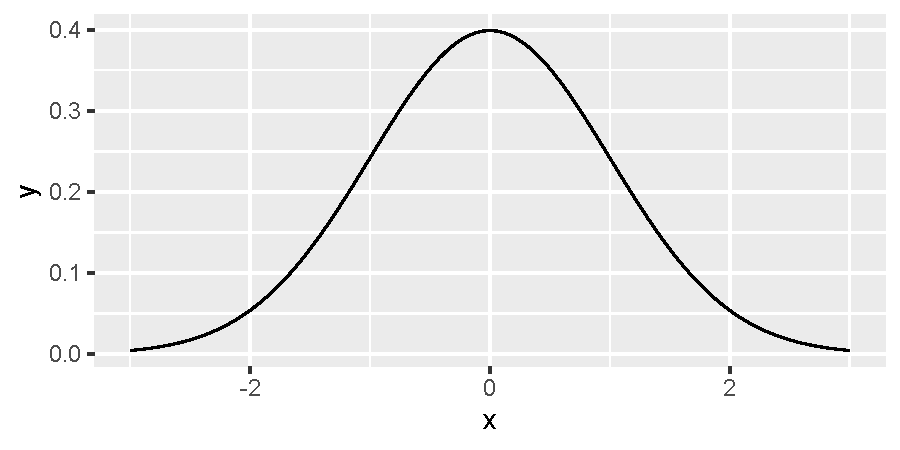
\includegraphics[width=.7\textwidth]{figure/pos-function-plot-01-1} 

}


\end{knitrout}

Using a list we can even pass by name additional arguments to use when the function is called.

\begin{knitrout}\footnotesize
\definecolor{shadecolor}{rgb}{0.969, 0.969, 0.969}\color{fgcolor}\begin{kframe}
\begin{alltt}
\hlkwd{ggplot}\hlstd{(}\hlkwd{data.frame}\hlstd{(}\hlkwc{x} \hlstd{=} \hlopt{-}\hlnum{3}\hlopt{:}\hlnum{3}\hlstd{),} \hlkwd{aes}\hlstd{(}\hlkwc{x} \hlstd{= x))} \hlopt{+}
  \hlkwd{stat_function}\hlstd{(}\hlkwc{fun} \hlstd{= dnorm,} \hlkwc{args} \hlstd{=} \hlkwd{list}\hlstd{(}\hlkwc{mean} \hlstd{=} \hlnum{1}\hlstd{,} \hlkwc{sd} \hlstd{=} \hlnum{.5}\hlstd{))}
\end{alltt}
\end{kframe}
\end{knitrout}

\begin{playground}
Edit the code above so as to plot in the same figure three curves, either for three different values for \code{mean} or for three different values for \code{sd}.
\end{playground}

Named user-defined functions (not shown), and anonymous functions (below) can also be used.

\begin{knitrout}\footnotesize
\definecolor{shadecolor}{rgb}{0.969, 0.969, 0.969}\color{fgcolor}\begin{kframe}
\begin{alltt}
\hlkwd{ggplot}\hlstd{(}\hlkwd{data.frame}\hlstd{(}\hlkwc{x} \hlstd{=} \hlnum{0}\hlopt{:}\hlnum{1}\hlstd{),} \hlkwd{aes}\hlstd{(}\hlkwc{x} \hlstd{= x))} \hlopt{+}
  \hlkwd{stat_function}\hlstd{(}\hlkwc{fun} \hlstd{=} \hlkwa{function}\hlstd{(}\hlkwc{x}\hlstd{,} \hlkwc{a}\hlstd{,} \hlkwc{b}\hlstd{)\{a} \hlopt{+} \hlstd{b} \hlopt{*} \hlstd{x}\hlopt{^}\hlnum{2}\hlstd{\},}
                \hlkwc{args} \hlstd{=} \hlkwd{list}\hlstd{(}\hlkwc{a} \hlstd{=} \hlnum{1}\hlstd{,} \hlkwc{b} \hlstd{=} \hlnum{1.4}\hlstd{))}
\end{alltt}
\end{kframe}
\end{knitrout}

\begin{playground}
Edit the code above to use a different function, such as $e^{x + k}$, adjusting the argument(s) passed through \code{args} accordingly. Do this by means of an anonymous function, and by means of an equivalent named function defined by your code.
\end{playground}

\index{plots!plots of functions|)}
\index{grammar of graphics!function statistic|)}

\subsection{Summaries}\label{sec:plot:stat:summaries}
\index{grammar of graphics!summary statistic|(}
\index{plots!data summaries|(}
\index{plots!means}\index{plots!medians}\index{plots!error bars}
The summaries discussed in this section can be superimposed on raw data plots, or plotted on their own. Beware, that if scale limits are manually set, the summaries will be calculated from the subset of observations within these limits. Scale limits can be altered when explicitly defining a scale or by means of functions \Rfunction{xlim()} and \Rfunction{ylim()}. See section \ref{sec:plot:coord} on page \pageref{sec:plot:coord} for an explanation of how coordinate limits can be used to zoom into a plot without excluding of $x$ and $y$ values from the data.

It is possible to summarize data on the fly when plotting. We describe in the same section the calculation of measures of central tendency and of variation, as \ggstat{stat\_summary()} allows them to be calculated simultaneously and added together with a single layer.

For use in the examples, we generate some normally distributed artificial data.

\begin{knitrout}\footnotesize
\definecolor{shadecolor}{rgb}{0.969, 0.969, 0.969}\color{fgcolor}\begin{kframe}
\begin{alltt}
\hlstd{fake.data} \hlkwb{<-} \hlkwd{data.frame}\hlstd{(}
  \hlkwc{y} \hlstd{=} \hlkwd{c}\hlstd{(}\hlkwd{rnorm}\hlstd{(}\hlnum{10}\hlstd{,} \hlkwc{mean} \hlstd{=} \hlnum{2}\hlstd{,} \hlkwc{sd} \hlstd{=} \hlnum{0.5}\hlstd{),}
        \hlkwd{rnorm}\hlstd{(}\hlnum{10}\hlstd{,} \hlkwc{mean} \hlstd{=} \hlnum{4}\hlstd{,} \hlkwc{sd} \hlstd{=} \hlnum{0.7}\hlstd{)),}
  \hlkwc{group} \hlstd{=} \hlkwd{factor}\hlstd{(}\hlkwd{c}\hlstd{(}\hlkwd{rep}\hlstd{(}\hlstr{"A"}\hlstd{,} \hlnum{10}\hlstd{),} \hlkwd{rep}\hlstd{(}\hlstr{"B"}\hlstd{,} \hlnum{10}\hlstd{)))}
  \hlstd{)}
\end{alltt}
\end{kframe}
\end{knitrout}

We will reuse a ``base'' scatter plot in a series of examples, so that the differences are easier to appreciate. We first add just the mean. In this case, we need to pass as an argument to \ggstat{stat\_summary()}, the \code{geom} to use, as the default one, \gggeom{geom\_pointrange()}, expects data for plotting error bars in addition to the mean. This example uses a hyphen character as the constant value of \code{shape} (see the example for \code{geom\_point()} on page \pageref{chunk:plot:point:char} on the use of digits as \code{shape}). Instead of passing \code{"mean"} as an argument to parameter \code{fun} (earlier called \code{fun.y}), we can pass, if desired, other summary functions like \code{"median"}. In the case of these functions that return a single computed value, we pass them, or character strings with their names, as an argument to parameter \code{fun}.

\begin{knitrout}\footnotesize
\definecolor{shadecolor}{rgb}{0.969, 0.969, 0.969}\color{fgcolor}\begin{kframe}
\begin{alltt}
\hlkwd{ggplot}\hlstd{(}\hlkwc{data} \hlstd{= fake.data,} \hlkwd{aes}\hlstd{(}\hlkwc{y} \hlstd{= y,} \hlkwc{x} \hlstd{= group))} \hlopt{+}
  \hlkwd{geom_point}\hlstd{(}\hlkwc{shape} \hlstd{=} \hlnum{21}\hlstd{)} \hlopt{+}
  \hlkwd{stat_summary}\hlstd{(}\hlkwc{fun} \hlstd{=} \hlstr{"mean"}\hlstd{,} \hlkwc{geom} \hlstd{=} \hlstr{"point"}\hlstd{,}
               \hlkwc{color} \hlstd{=} \hlstr{"red"}\hlstd{,} \hlkwc{shape} \hlstd{=} \hlstr{"-"}\hlstd{,} \hlkwc{size} \hlstd{=} \hlnum{10}\hlstd{)}
\end{alltt}
\end{kframe}

{\centering 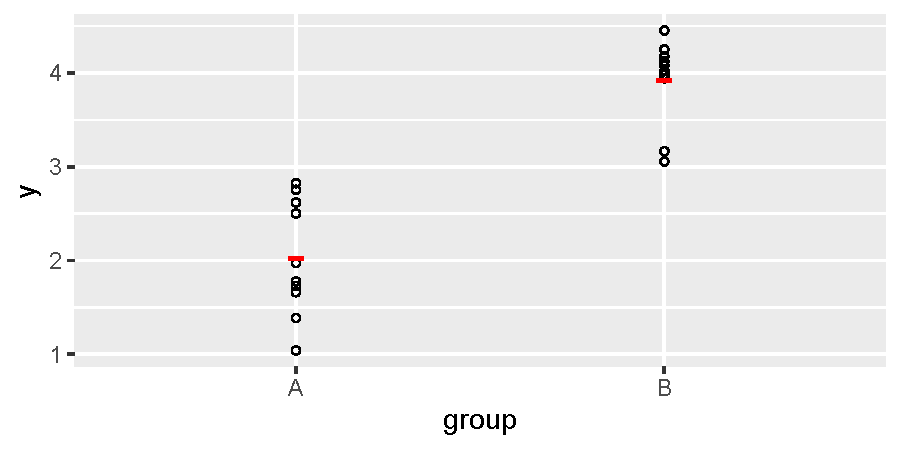
\includegraphics[width=.7\textwidth]{figure/pos-summary-plot-02-1} 

}


\end{knitrout}

To pass as an argument a function that returns a central value like the mean plus confidence or other limits, we use parameter \code{fun.data} instead of \code{fun}. In the next example we add means and confidence intervals for $p = 0.95$ (the default) assuming normality.

\begin{knitrout}\footnotesize
\definecolor{shadecolor}{rgb}{0.969, 0.969, 0.969}\color{fgcolor}\begin{kframe}
\begin{alltt}
  \hlkwd{stat_summary}\hlstd{(}\hlkwc{fun.data} \hlstd{=} \hlstr{"mean_cl_normal"}\hlstd{,} \hlkwc{color} \hlstd{=} \hlstr{"red"}\hlstd{,} \hlkwc{size} \hlstd{=} \hlnum{1}\hlstd{,} \hlkwc{alpha} \hlstd{=} \hlnum{0.7}\hlstd{)}
\end{alltt}
\end{kframe}
\end{knitrout}

We can override the default of $p = 0.95$ for confidence intervals by setting, for example, \code{conf.int = 0.90} in the list of arguments passed to the function. The intervals can also be computed without assuming normality, using the empirical distribution estimated from the data by bootstrap. To achieve this we pass to \code{fun.data} the argument \code{"mean\_cl\_boot"} instead of \code{"mean\_cl\_normal"}.

\begin{knitrout}\footnotesize
\definecolor{shadecolor}{rgb}{0.969, 0.969, 0.969}\color{fgcolor}\begin{kframe}
\begin{alltt}
  \hlkwd{stat_summary}\hlstd{(}\hlkwc{fun.data} \hlstd{=} \hlstr{"mean_cl_boot"}\hlstd{,}
               \hlkwc{fun.args} \hlstd{=} \hlkwd{list}\hlstd{(}\hlkwc{conf.int} \hlstd{=} \hlnum{0.90}\hlstd{),}
               \hlkwc{color} \hlstd{=} \hlstr{"red"}\hlstd{,} \hlkwc{size} \hlstd{=} \hlnum{1}\hlstd{,} \hlkwc{alpha} \hlstd{=} \hlnum{0.7}\hlstd{)}
\end{alltt}
\end{kframe}
\end{knitrout}

For $\bar{x} \pm \mathrm{s.e.}$ we should pass \code{"mean\_se"} and for $\bar{x} \pm \mathrm{s.d.}$ \code{"mean\_sdl"}.

\begin{knitrout}\footnotesize
\definecolor{shadecolor}{rgb}{0.969, 0.969, 0.969}\color{fgcolor}\begin{kframe}
\begin{alltt}
  \hlkwd{stat_summary}\hlstd{(}\hlkwc{fun.data} \hlstd{=} \hlstr{"mean_se"}\hlstd{,}
               \hlkwc{color} \hlstd{=} \hlstr{"red"}\hlstd{,} \hlkwc{size} \hlstd{=} \hlnum{1}\hlstd{,} \hlkwc{alpha} \hlstd{=} \hlnum{0.7}\hlstd{)}
\end{alltt}
\end{kframe}
\end{knitrout}

We do not give an example here, but it is possible to use user-defined functions instead of the functions exported by package \ggplot (based on those in package \Hmisc). Because arguments to the function used, except for the first one containing the variable in \code{data} mapped to the $y$ aesthetic, are supplied as a named list through parameter \code{fun.args}, the names used for parameters in the function definition need only match the names in this list.

Finally, we plot the means in a scatter plot, with the observations superimposed on the error bars as a result of the order in which the layers are added to the plot. In this case, we set \code{fill}, \code{color} and \code{alpha} (transparency) to constants, but in more complex data sets, mapping them to factors in \code{data} can be used for grouping of observations. Here, adding two plot layers with \ggstat{stat\_summary()} allows us to plot the mean and the error bars using different colors.

\begin{knitrout}\footnotesize
\definecolor{shadecolor}{rgb}{0.969, 0.969, 0.969}\color{fgcolor}\begin{kframe}
\begin{alltt}
\hlkwd{ggplot}\hlstd{(}\hlkwc{data} \hlstd{= fake.data,} \hlkwd{aes}\hlstd{(}\hlkwc{y} \hlstd{= y,} \hlkwc{x} \hlstd{= group))} \hlopt{+}
  \hlkwd{stat_summary}\hlstd{(}\hlkwc{fun} \hlstd{=} \hlstr{"mean"}\hlstd{,} \hlkwc{geom} \hlstd{=} \hlstr{"point"}\hlstd{,}
               \hlkwc{fill} \hlstd{=} \hlstr{"white"}\hlstd{,} \hlkwc{color} \hlstd{=} \hlstr{"black"}\hlstd{)} \hlopt{+}
  \hlkwd{stat_summary}\hlstd{(}\hlkwc{fun.data} \hlstd{=} \hlstr{"mean_cl_boot"}\hlstd{,}
               \hlkwc{geom} \hlstd{=} \hlstr{"errorbar"}\hlstd{,}
               \hlkwc{width} \hlstd{=} \hlnum{0.1}\hlstd{,} \hlkwc{size} \hlstd{=} \hlnum{1}\hlstd{,} \hlkwc{color} \hlstd{=} \hlstr{"red"}\hlstd{)} \hlopt{+}
  \hlkwd{geom_point}\hlstd{(}\hlkwc{size} \hlstd{=} \hlnum{3}\hlstd{,} \hlkwc{alpha} \hlstd{=} \hlnum{0.3}\hlstd{)}
\end{alltt}
\end{kframe}
\end{knitrout}

We can plot means, or other summaries, by group mapped to \code{x} (\code{class} in this example) as columns by passing \code{"col"} as an argument to  \code{geom}. In this way we avoid the need to compute the summaries in advance.

\begin{knitrout}\footnotesize
\definecolor{shadecolor}{rgb}{0.969, 0.969, 0.969}\color{fgcolor}\begin{kframe}
\begin{alltt}
\hlkwd{ggplot}\hlstd{(mpg,} \hlkwd{aes}\hlstd{(class, hwy))} \hlopt{+}
  \hlkwd{stat_summary}\hlstd{(}\hlkwc{geom} \hlstd{=} \hlstr{"col"}\hlstd{,} \hlkwc{fun} \hlstd{= mean)}
\end{alltt}
\end{kframe}

{\centering 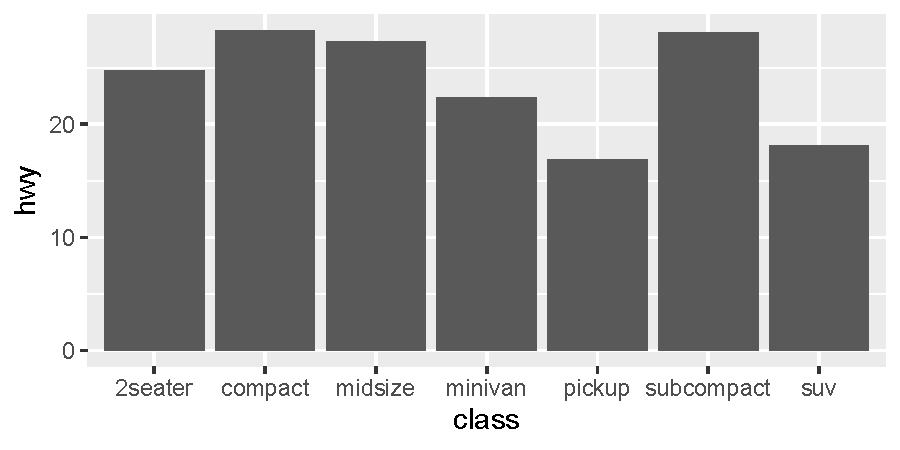
\includegraphics[width=.7\textwidth]{figure/pos-summary-plot-09a-1} 

}


\end{knitrout}

We can easily add error bars to the column plot. We use \code{size} to make the lines of the error bars thicker. The default \emph{geometry} in \ggstat{stat\_summary()} is \gggeom{geom\_pointrange()}, so we can pass \code{"linerange"} as an argument for \code{geom} to eliminate the point.

\begin{knitrout}\footnotesize
\definecolor{shadecolor}{rgb}{0.969, 0.969, 0.969}\color{fgcolor}\begin{kframe}
\begin{alltt}
  \hlkwd{stat_summary}\hlstd{(}\hlkwc{geom} \hlstd{=} \hlstr{"linerange"}\hlstd{,} \hlkwc{fun.data} \hlstd{=} \hlstr{"mean_se"}\hlstd{,}
               \hlkwc{size} \hlstd{=} \hlnum{1}\hlstd{,} \hlkwc{color} \hlstd{=} \hlstr{"red"}\hlstd{)}
\end{alltt}
\end{kframe}
\end{knitrout}

Passing \code{"errorbar"} instead of \code{"linerange"} to \code{geom} results in traditional ``capped'' error bars. However, this type of error bar has been criticized as adding unnecessary clutter to plots \autocite{Tufte1983}. We can use \code{width} to reduce the width of the caps at the ends of the error bars.

If we have already calculated values for the summaries, we can still obtain the same plots by mapping variables to the \emph{aesthetics} required by \gggeom{geom\_errorbar()} and \gggeom{geom\_linerange()}: \code{x}, \code{y}, \code{ymax} and \code{ymin}.

\begin{explainbox}
The ``reverse'' syntax is also valid, as we can add the \emph{geometry} to the plot object and pass the \emph{statistics} as an argument to it. In general in this book we avoid this alternative syntax for the sake of consistency.

\begin{knitrout}\footnotesize
\definecolor{shadecolor}{rgb}{0.969, 0.969, 0.969}\color{fgcolor}\begin{kframe}
\begin{alltt}
\hlkwd{ggplot}\hlstd{(mpg,} \hlkwd{aes}\hlstd{(class, hwy))} \hlopt{+}
  \hlkwd{geom_col}\hlstd{(}\hlkwc{stat} \hlstd{=} \hlstr{"summary"}\hlstd{,} \hlkwc{fun} \hlstd{= mean)}
\end{alltt}
\end{kframe}
\end{knitrout}
\end{explainbox}
\index{plots!data summaries|)}
\index{grammar of graphics!summary statistic|)}

\subsection{Smoothers and models}\label{sec:plot:smoothers}
\index{plots!smooth curves|(}
\index{plots!fitted curves|(}
\index{plots!statistics!smooth}
The \emph{statistic} \ggstat{stat\_smooth()} fits a smooth curve to observations in the case when the scales for $x$ and $y$ are continuous---the corresponding \emph{geometry} \gggeom{geom\_smooth()} uses this \emph{statistic}, and differs only in how arguments are passed to formal parameters. For the first example, we use \ggstat{stat\_smooth()} with the default smoother, a spline. The type of spline is automatically chosen based on the number of observations and informed by a message. The \code{formula} must be stated using the names of the $x$ and $y$ aesthetics, rather the names of the mapped variables in \code{mtcars}.

\begin{knitrout}\footnotesize
\definecolor{shadecolor}{rgb}{0.969, 0.969, 0.969}\color{fgcolor}\begin{kframe}
\begin{alltt}
\hlkwd{ggplot}\hlstd{(}\hlkwc{data} \hlstd{= mtcars,} \hlkwd{aes}\hlstd{(}\hlkwc{x} \hlstd{= disp,} \hlkwc{y} \hlstd{= mpg))} \hlopt{+}
       \hlkwd{stat_smooth}\hlstd{(}\hlkwc{formula} \hlstd{= y} \hlopt{~} \hlstd{x)}
\end{alltt}
\end{kframe}
\end{knitrout}

In most cases we will want to plot the observations as points together with the smoother. We can plot the observation on top of the smoother, as done here, or the smoother on top of the observations.

\begin{knitrout}\footnotesize
\definecolor{shadecolor}{rgb}{0.969, 0.969, 0.969}\color{fgcolor}\begin{kframe}
\begin{alltt}
\hlkwd{ggplot}\hlstd{(}\hlkwc{data} \hlstd{= mtcars,} \hlkwd{aes}\hlstd{(}\hlkwc{x} \hlstd{= disp,} \hlkwc{y} \hlstd{= mpg))} \hlopt{+}
  \hlkwd{stat_smooth}\hlstd{(}\hlkwc{formula} \hlstd{= y} \hlopt{~} \hlstd{x)} \hlopt{+}
  \hlkwd{geom_point}\hlstd{()}
\end{alltt}


{\ttfamily\noindent\itshape\color{messagecolor}{\#\# `geom\_smooth()` using method = 'loess'}}\end{kframe}

{\centering 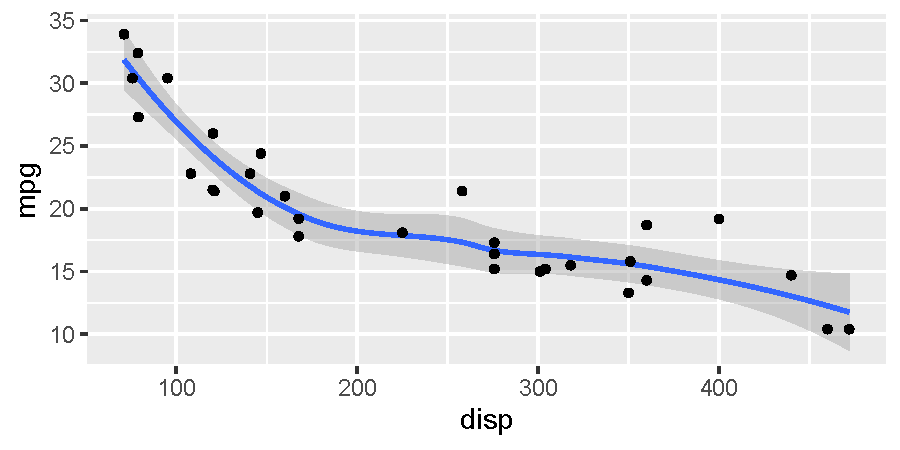
\includegraphics[width=.7\textwidth]{figure/pos-smooth-plot-02-1} 

}


\end{knitrout}

Instead of using the default spline, we can fit a different model. In this example we use a linear model as smoother, fitted by \Rfunction{lm()}.

\begin{knitrout}\footnotesize
\definecolor{shadecolor}{rgb}{0.969, 0.969, 0.969}\color{fgcolor}\begin{kframe}
\begin{alltt}
  \hlkwd{stat_smooth}(method = \hlstr{"lm"}, formula = y ~ x) +
\end{alltt}
\end{kframe}
\end{knitrout}

These data are really grouped, so we map variable \code{cyl} to the \code{color} \emph{aesthetic}. Now we get three groups of points with different colours but also three separate smooth lines.

\begin{knitrout}\footnotesize
\definecolor{shadecolor}{rgb}{0.969, 0.969, 0.969}\color{fgcolor}\begin{kframe}
\begin{alltt}
\hlkwd{ggplot}\hlstd{(}\hlkwc{data} \hlstd{= mtcars,} \hlkwd{aes}\hlstd{(}\hlkwc{x} \hlstd{= disp,} \hlkwc{y} \hlstd{= mpg,} \hlkwc{color} \hlstd{=} \hlkwd{factor}\hlstd{(cyl)))} \hlopt{+}
  \hlkwd{stat_smooth}\hlstd{(}\hlkwc{method} \hlstd{=} \hlstr{"lm"}\hlstd{,} \hlkwc{formula} \hlstd{= y} \hlopt{~} \hlstd{x)} \hlopt{+}
  \hlkwd{geom_point}\hlstd{()}
\end{alltt}
\end{kframe}

{\centering 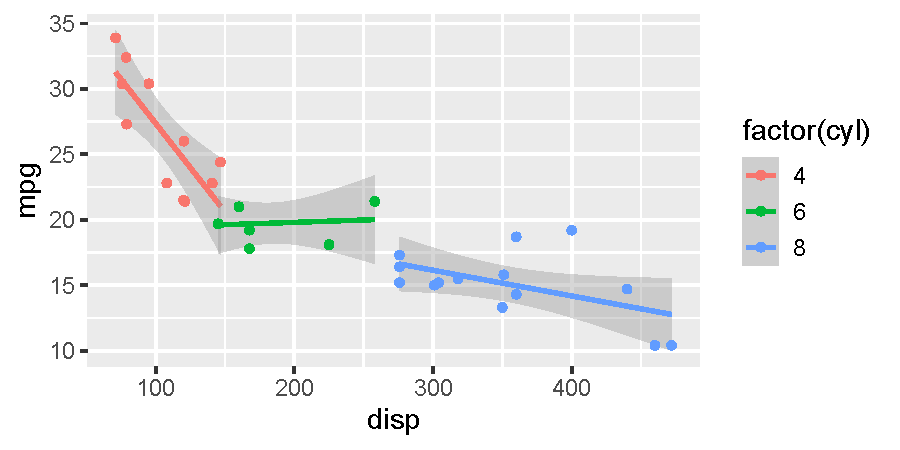
\includegraphics[width=.7\textwidth]{figure/pos-smooth-plot-04-1} 

}


\end{knitrout}

To obtain a single smoother for the three groups, we need to set the mapping of the \code{color} \emph{aesthetic} to a constant within \ggstat{stat\_smooth()}. This local value overrides the default \code{color} mapping set in \code{ggplot()} just for this plot layer. We use \code{"black"} but this could be replaced by any other color definition known to \Rlang.

\begin{knitrout}\footnotesize
\definecolor{shadecolor}{rgb}{0.969, 0.969, 0.969}\color{fgcolor}\begin{kframe}
\begin{alltt}
\hlkwd{ggplot}\hlstd{(}\hlkwc{data} \hlstd{= mtcars,} \hlkwd{aes}\hlstd{(}\hlkwc{x} \hlstd{= disp,} \hlkwc{y} \hlstd{= mpg,} \hlkwc{color} \hlstd{=} \hlkwd{factor}\hlstd{(cyl)))} \hlopt{+}
  \hlkwd{stat_smooth}\hlstd{(}\hlkwc{method} \hlstd{=} \hlstr{"lm"}\hlstd{,} \hlkwc{formula} \hlstd{= y} \hlopt{~} \hlstd{x,} \hlkwc{color} \hlstd{=} \hlstr{"black"}\hlstd{)} \hlopt{+}
  \hlkwd{geom_point}\hlstd{()}
\end{alltt}
\end{kframe}
\end{knitrout}

Instead of using the \code{formula} for a linear regression as smoother, we pass a different \code{formula} as an argument. In this example we use a polynomial of order 2.

\begin{knitrout}\footnotesize
\definecolor{shadecolor}{rgb}{0.969, 0.969, 0.969}\color{fgcolor}\begin{kframe}
\begin{alltt}
\hlkwd{ggplot}\hlstd{(}\hlkwc{data} \hlstd{= mtcars,} \hlkwd{aes}\hlstd{(}\hlkwc{x} \hlstd{= disp,} \hlkwc{y} \hlstd{= mpg,} \hlkwc{color} \hlstd{=} \hlkwd{factor}\hlstd{(cyl)))} \hlopt{+}
  \hlkwd{stat_smooth}\hlstd{(}\hlkwc{method} \hlstd{=} \hlstr{"lm"}\hlstd{,} \hlkwc{formula} \hlstd{= y} \hlopt{~} \hlkwd{poly}\hlstd{(x,} \hlnum{2}\hlstd{),} \hlkwc{color} \hlstd{=} \hlstr{"black"}\hlstd{)} \hlopt{+}
  \hlkwd{geom_point}\hlstd{()}
\end{alltt}
\end{kframe}

{\centering 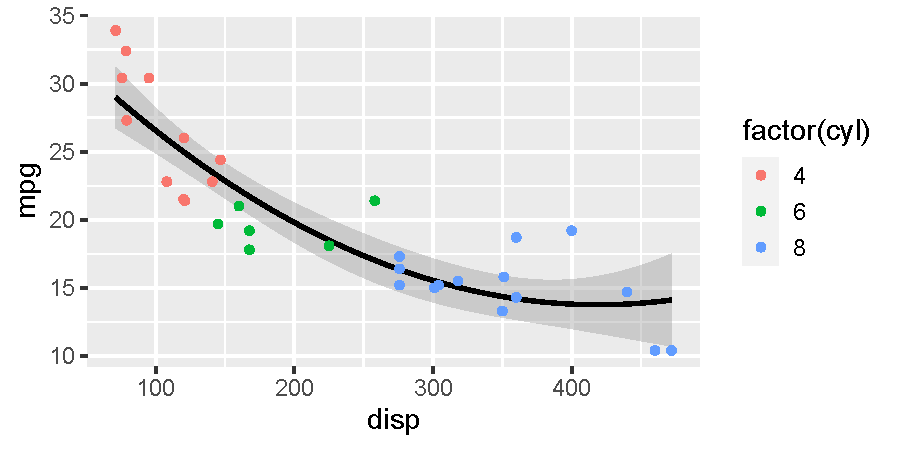
\includegraphics[width=.7\textwidth]{figure/pos-smooth-plot-06-1} 

}


\end{knitrout}

It is possible to use other types of models, including GAM and GLM, as smoothers, but we will give only two simple examples of the use of \code{nls()} to fit a model non-linear in its parameters (see section \ref{sec:stat:NLS} on page \pageref{sec:stat:NLS} for details about fitting this same model with \code{nls()}). In the first one we fit a Michaelis-Menten equation to reaction rate (\code{rate}) versus reactant concentration (\code{conc}). \Rdata{Puromycin} is a data set included in the \Rlang distribution. Function \Rfunction{SSmicmen()} is also from \Rlang, and is a \emph{self-starting}\index{self-starting functions} implementation of the Michaelis-Menten equation. Thanks to this, even though the fit is done with an iterative algorithm, we do not need to explicitly provide starting values for the parameters to be fitted. We need to set \code{se = FALSE} because standard errors are not supported by the \code{predict()} method for \code{nls} fitted models.

\begin{knitrout}\footnotesize
\definecolor{shadecolor}{rgb}{0.969, 0.969, 0.969}\color{fgcolor}\begin{kframe}
\begin{alltt}
\hlkwd{ggplot}\hlstd{(Puromycin,} \hlkwd{aes}\hlstd{(conc, rate,} \hlkwc{color} \hlstd{= state))} \hlopt{+}
  \hlkwd{geom_point}\hlstd{()} \hlopt{+}
  \hlkwd{geom_smooth}\hlstd{(}\hlkwc{method} \hlstd{=} \hlstr{"nls"}\hlstd{,}
              \hlkwc{formula} \hlstd{=  y} \hlopt{~} \hlkwd{SSmicmen}\hlstd{(x, Vm, K),}
              \hlkwc{se} \hlstd{=} \hlnum{FALSE}\hlstd{)}
\end{alltt}
\end{kframe}
\end{knitrout}

In the second example we define the same model directly in the model formula, and provide the starting values explicitly. The names used for the parameters to be fitted can be chosen at will, within the restrictions of the \Rlang language, but of course the names used in \code{formula} and \code{start} must match each other.

\begin{knitrout}\footnotesize
\definecolor{shadecolor}{rgb}{0.969, 0.969, 0.969}\color{fgcolor}\begin{kframe}
\begin{alltt}
\hlkwd{ggplot}\hlstd{(Puromycin,} \hlkwd{aes}\hlstd{(conc, rate,} \hlkwc{color} \hlstd{= state))} \hlopt{+}
  \hlkwd{geom_point}\hlstd{()} \hlopt{+}
  \hlkwd{geom_smooth}\hlstd{(}\hlkwc{method} \hlstd{=} \hlstr{"nls"}\hlstd{,}
              \hlkwc{method.args} \hlstd{=} \hlkwd{list}\hlstd{(}\hlkwc{formula} \hlstd{=  y} \hlopt{~} \hlstd{(Vmax} \hlopt{*} \hlstd{x)} \hlopt{/} \hlstd{(k} \hlopt{+} \hlstd{x),}
                                 \hlkwc{start} \hlstd{=} \hlkwd{list}\hlstd{(}\hlkwc{Vmax} \hlstd{=} \hlnum{200}\hlstd{,} \hlkwc{k} \hlstd{=} \hlnum{0.05}\hlstd{)),}
              \hlkwc{se} \hlstd{=} \hlnum{FALSE}\hlstd{)}
\end{alltt}
\end{kframe}
\end{knitrout}

In some cases it is desirable to annotate plots with fitted model equations or fitted parameters. One way of achieving this is by fitting the model and then extracting the parameters to manually construct text strings to use for text or label annotations. However, package \pkgname{ggpmisc} makes it possible to automate such annotations in many cases. This package also provides \ggstat{stat\_poly\_line()} which is similar to \ggstat{stat\_smooth()} but with \code{method = "lm"} consistently as its default irrespective of the number of observations.

\begin{knitrout}\footnotesize
\definecolor{shadecolor}{rgb}{0.969, 0.969, 0.969}\color{fgcolor}\begin{kframe}
\begin{alltt}
\hlstd{my.formula} \hlkwb{<-} \hlstd{y} \hlopt{~} \hlkwd{poly}\hlstd{(x,} \hlnum{2}\hlstd{)}
\hlkwd{ggplot}\hlstd{(}\hlkwc{data} \hlstd{= mtcars,} \hlkwd{aes}\hlstd{(}\hlkwc{x} \hlstd{= disp,} \hlkwc{y} \hlstd{= mpg,} \hlkwc{color} \hlstd{=} \hlkwd{factor}\hlstd{(cyl)))} \hlopt{+}
  \hlkwd{stat_poly_line}\hlstd{(}\hlkwc{formula} \hlstd{= my.formula,} \hlkwc{color} \hlstd{=} \hlstr{"black"}\hlstd{)} \hlopt{+}
  \hlkwd{stat_poly_eq}\hlstd{(}\hlkwc{formula} \hlstd{= my.formula,} \hlkwd{aes}\hlstd{(}\hlkwc{label} \hlstd{= ..eq.label..),}
               \hlkwc{color} \hlstd{=} \hlstr{"black"}\hlstd{,} \hlkwc{parse} \hlstd{=} \hlnum{TRUE}\hlstd{,} \hlkwc{label.x.npc} \hlstd{=} \hlnum{0.3}\hlstd{)} \hlopt{+}
  \hlkwd{geom_point}\hlstd{()}
\end{alltt}


{\ttfamily\noindent\color{warningcolor}{\#\# Warning: The dot-dot notation (`..eq.label..`) was deprecated in ggplot2 3.4.0.\\\#\# i Please use `after\_stat(eq.label)` instead.}}\end{kframe}

{\centering 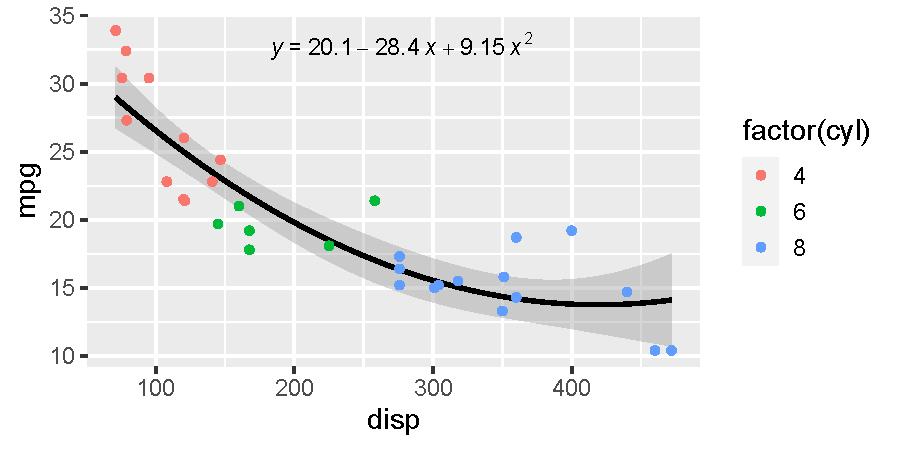
\includegraphics[width=.7\textwidth]{figure/pos-smooth-plot-12-1} 

}


\end{knitrout}

This same package makes it possible to annotate plots with summary tables from a model fit.

\begin{knitrout}\footnotesize
\definecolor{shadecolor}{rgb}{0.969, 0.969, 0.969}\color{fgcolor}\begin{kframe}
\begin{alltt}
\hlstd{my.formula} \hlkwb{<-} \hlstd{y} \hlopt{~} \hlkwd{poly}\hlstd{(x,} \hlnum{2}\hlstd{)}
\hlkwd{ggplot}\hlstd{(}\hlkwc{data} \hlstd{= mtcars,} \hlkwd{aes}\hlstd{(}\hlkwc{x} \hlstd{= disp,} \hlkwc{y} \hlstd{= mpg,} \hlkwc{color} \hlstd{=} \hlkwd{factor}\hlstd{(cyl)))} \hlopt{+}
  \hlkwd{stat_poly_line}\hlstd{(}\hlkwc{formula} \hlstd{= my.formula,} \hlkwc{color} \hlstd{=} \hlstr{"black"}\hlstd{)} \hlopt{+}
  \hlkwd{stat_fit_tb}\hlstd{(}\hlkwc{method.args} \hlstd{=} \hlkwd{list}\hlstd{(}\hlkwc{formula} \hlstd{= my.formula),}
              \hlkwc{color} \hlstd{=} \hlstr{"black"}\hlstd{,}
              \hlkwc{tb.vars} \hlstd{=} \hlkwd{c}\hlstd{(}\hlkwc{Parameter} \hlstd{=} \hlstr{"term"}\hlstd{,}
                          \hlkwc{Estimate} \hlstd{=} \hlstr{"estimate"}\hlstd{,}
                          \hlstr{"s.e."} \hlstd{=} \hlstr{"std.error"}\hlstd{,}
                          \hlstr{"italic(t)"} \hlstd{=} \hlstr{"statistic"}\hlstd{,}
                          \hlstr{"italic(P)"} \hlstd{=} \hlstr{"p.value"}\hlstd{),}
              \hlkwc{label.y.npc} \hlstd{=} \hlstr{"top"}\hlstd{,} \hlkwc{label.x.npc} \hlstd{=} \hlstr{"right"}\hlstd{,}
              \hlkwc{parse} \hlstd{=} \hlnum{TRUE}\hlstd{)} \hlopt{+}
  \hlkwd{geom_point}\hlstd{()}
\end{alltt}


{\ttfamily\noindent\color{warningcolor}{\#\# Warning: Computation failed in `stat\_fit\_tb()`\\\#\# Caused by error in `UseMethod()`:\\\#\# ! no applicable method for 'tidy' applied to an object of class "{}lm"{}}}\end{kframe}

{\centering 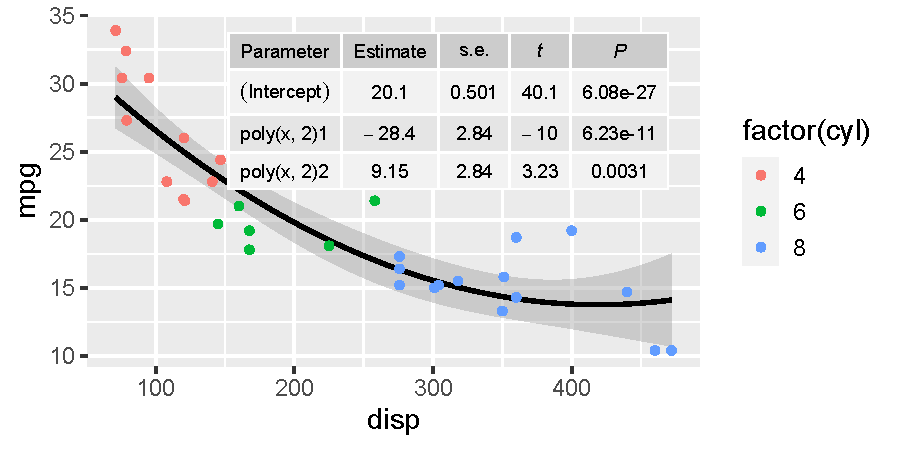
\includegraphics[width=.7\textwidth]{figure/pos-smooth-plot-13-1} 

}


\end{knitrout}

Package \pkgname{ggpmisc} provides additional \emph{statistics} for the annotation of plots based on fitted models supported by package \pkgname{broom} and its extensions. It also supports lines and equations for quantile regression and major axis regression. Please see the package documentation for details.

\index{plots!smooth curves|)}
\index{plots!fitted curves|)}

\subsection{Frequencies and counts}\label{sec:histogram}\label{sec:plot:histogram}
\index{plots!histograms|(}

When the number of observations is rather small, we can rely on the density of graphical elements to convey the density of the observations. For example, scatter plots using well-chosen values for \code{alpha} can give a satisfactory impression of the density. Rug plots, described in section \ref{sec:plot:rug} on page \pageref{sec:plot:rug}, can also satisfactorily convey the density of observations along $x$ and/or $y$ axes. Such approaches do not involve computations, while the \emph{statistics} described in this section do. Frequencies by value-range (or bins) and empirical density functions are summaries especially useful when the number of observations is large. These summaries can be computed in one or more dimensions.

Histograms are defined by how the plotted values are calculated. Although histograms are most frequently plotted as bar plots, many bar or ``column'' plots are not histograms. Although rarely done in practice, a histogram could be plotted using a different \emph{geometry} using \ggstat{stat\_bin()}, the \emph{statistic} used by default by \gggeom{geom\_histogram()}. This \emph{statistic} does binning of observations before computing frequencies, and is suitable for continuous $x$ scales. When a factor is mapped to \code{x}, \ggstat{stat\_count()} should be used, which is the default \code{stat} for \gggeom{geom\_bar()}. These two \emph{geometries} are described in this section about statistics, because they default to using statistics different from \code{stat\_identity()} and consequently summarize the data.

As before, we generate suitable artificial data.

\begin{knitrout}\footnotesize
\definecolor{shadecolor}{rgb}{0.969, 0.969, 0.969}\color{fgcolor}\begin{kframe}
\begin{alltt}
\hlkwd{set.seed}\hlstd{(}\hlnum{12345}\hlstd{)}
\hlstd{my.data} \hlkwb{<-}
  \hlkwd{data.frame}\hlstd{(}\hlkwc{x} \hlstd{=} \hlkwd{rnorm}\hlstd{(}\hlnum{200}\hlstd{),}
             \hlkwc{y} \hlstd{=} \hlkwd{c}\hlstd{(}\hlkwd{rnorm}\hlstd{(}\hlnum{100}\hlstd{,} \hlopt{-}\hlnum{1}\hlstd{,} \hlnum{1}\hlstd{),} \hlkwd{rnorm}\hlstd{(}\hlnum{100}\hlstd{,} \hlnum{1}\hlstd{,} \hlnum{1}\hlstd{)),}
             \hlkwc{group} \hlstd{=} \hlkwd{factor}\hlstd{(}\hlkwd{rep}\hlstd{(}\hlkwd{c}\hlstd{(}\hlstr{"A"}\hlstd{,} \hlstr{"B"}\hlstd{),} \hlkwd{c}\hlstd{(}\hlnum{100}\hlstd{,} \hlnum{100}\hlstd{))) )}
\end{alltt}
\end{kframe}
\end{knitrout}

We could have relied on the default number of bins automatically computed by the \ggstat{stat\_bin()} statistic, however, we here set it to 15 with \code{bins = 15}. It is important to remember that in this case no variable in \code{data} is mapped onto the \code{y} \emph{aesthetic}.

\begin{knitrout}\footnotesize
\definecolor{shadecolor}{rgb}{0.969, 0.969, 0.969}\color{fgcolor}\begin{kframe}
\begin{alltt}
\hlkwd{ggplot}\hlstd{(my.data,} \hlkwd{aes}\hlstd{(x))} \hlopt{+}
  \hlkwd{geom_histogram}\hlstd{(}\hlkwc{bins} \hlstd{=} \hlnum{15}\hlstd{)}
\end{alltt}
\end{kframe}

{\centering 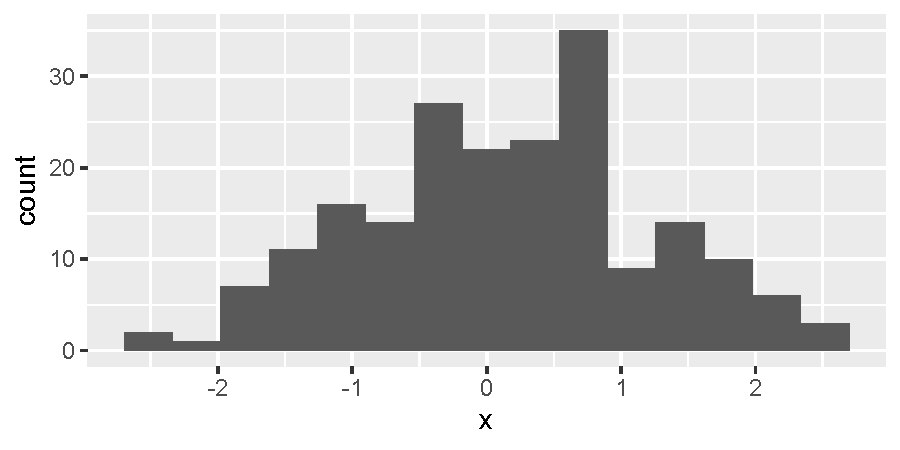
\includegraphics[width=.7\textwidth]{figure/pos-histogram-plot-01-1} 

}


\end{knitrout}

If we create a grouping by mapping a factor to an additional \emph{aesthetic} how the bars created are positioned with respect to each other becomes relevant. We can then plot side by side with \code{position = "dodge"}, stacked one above the other with \code{position = "stack"} and overlapping with \code{position = "identity"} in which case we need to make them semi-transparent with \code{alpha = 0.5} so that they all remain visible.

\begin{knitrout}\footnotesize
\definecolor{shadecolor}{rgb}{0.969, 0.969, 0.969}\color{fgcolor}\begin{kframe}
\begin{alltt}
\hlkwd{ggplot}\hlstd{(my.data,} \hlkwd{aes}\hlstd{(y,} \hlkwc{fill} \hlstd{= group))} \hlopt{+}
  \hlkwd{geom_histogram}\hlstd{(}\hlkwc{bins} \hlstd{=} \hlnum{15}\hlstd{,} \hlkwc{position} \hlstd{=} \hlstr{"dodge"}\hlstd{)}
\end{alltt}
\end{kframe}
\end{knitrout}

The computed values are contained in the \code{data} that the \emph{geometry} ``receives'' from the \emph{statistic}. Many statistics compute additional values that are not mapped by default. These can be mapped with \code{aes()} by enclosing them in a call to \code{stat()}. From the help page we can learn that in addition to counts in variable \code{count}, density is returned in variable \code{density} by this statistic. Consequently, we can create a histogram with the counts per bin expressed as densities whose integral is one (rather than their sum, as the width of the bins is in this case different from one), as follows.

\begin{knitrout}\footnotesize
\definecolor{shadecolor}{rgb}{0.969, 0.969, 0.969}\color{fgcolor}\begin{kframe}
\begin{alltt}
\hlkwd{ggplot}\hlstd{(my.data,} \hlkwd{aes}\hlstd{(y,} \hlkwc{fill} \hlstd{= group))} \hlopt{+}
  \hlkwd{geom_histogram}\hlstd{(}\hlkwc{mapping} \hlstd{=} \hlkwd{aes}\hlstd{(}\hlkwc{y} \hlstd{=} \hlkwd{stat}\hlstd{(density)),} \hlkwc{bins} \hlstd{=} \hlnum{15}\hlstd{,} \hlkwc{position} \hlstd{=} \hlstr{"dodge"}\hlstd{)}
\end{alltt}


{\ttfamily\noindent\color{warningcolor}{\#\# Warning: `stat(density)` was deprecated in ggplot2 3.4.0.\\\#\# i Please use `after\_stat(density)` instead.}}\end{kframe}

{\centering \includegraphics[width=.7\textwidth]{figure/pos-histogram-plot-03-1} 

}


\end{knitrout}

If it were not for the easier to remember name of \gggeom{geom\_histogram()}, adding the layers with \ggstat{stat\_bin()} or \ggstat{stat\_count()} would be preferable as it makes clear that computations on the data are involved.

\begin{knitrout}\footnotesize
\definecolor{shadecolor}{rgb}{0.969, 0.969, 0.969}\color{fgcolor}\begin{kframe}
\begin{alltt}
\hlkwd{ggplot}\hlstd{(my.data,} \hlkwd{aes}\hlstd{(y,} \hlkwc{fill} \hlstd{= group))} \hlopt{+}
  \hlkwd{stat_bin}\hlstd{(}\hlkwc{bins} \hlstd{=} \hlnum{15}\hlstd{,} \hlkwc{position} \hlstd{=} \hlstr{"dodge"}\hlstd{)}
\end{alltt}
\end{kframe}
\end{knitrout}

The \emph{statistic} \ggstat{stat\_bin2d()}, and its matching \emph{geometry} \gggeom{geom\_bin2d()}, by default compute a frequency histogram in two dimensions, along the \code{x} and \code{y} \emph{aesthetics}. The frequency for each rectangular tile is mapped onto a \code{fill} scale. As for \ggstat{stat\_bin()}, \code{density} is also computed and available to be mapped as shown above for \code{geom\_histogram}. In this example, to compare dispersion in two dimensions, equal $x$ and $y$ scales are most suitable, which we achieve by adding \ggcoordinate{coord\_fixed()}, which is a variation of the default \ggcoordinate{coord\_cartesian()}  (see section \ref{sec:plot:coord} on page \pageref{sec:plot:coord} for details on other systems of coordinates).

\begin{knitrout}\footnotesize
\definecolor{shadecolor}{rgb}{0.969, 0.969, 0.969}\color{fgcolor}\begin{kframe}
\begin{alltt}
\hlkwd{ggplot}\hlstd{(my.data,} \hlkwd{aes}\hlstd{(x, y))} \hlopt{+}
  \hlkwd{stat_bin2d}\hlstd{(}\hlkwc{bins} \hlstd{=} \hlnum{8}\hlstd{)} \hlopt{+}
  \hlkwd{coord_fixed}\hlstd{(}\hlkwc{ratio} \hlstd{=} \hlnum{1}\hlstd{)}
\end{alltt}
\end{kframe}

{\centering \includegraphics[width=.7\textwidth]{figure/pos-bin2d-plot-01-1} 

}


\end{knitrout}

The \emph{statistic} \ggstat{stat\_bin\_hex()}, and its matching \emph{geometry} \gggeom{geom\_hex()}, differ from \ggstat{stat\_bin2d()} in their use of hexagonal instead of square tiles. By default the frequency or \code{count} for each hexagon is mapped to the \code{fill} aesthetic, but counts expressed as \code{density} are also computed and can be mapped with \code{aes(fill = stat(density))}.

\begin{knitrout}\footnotesize
\definecolor{shadecolor}{rgb}{0.969, 0.969, 0.969}\color{fgcolor}\begin{kframe}
\begin{alltt}
\hlkwd{ggplot}\hlstd{(my.data,} \hlkwd{aes}\hlstd{(x, y))} \hlopt{+}
  \hlkwd{stat_bin_hex}\hlstd{(}\hlkwc{bins} \hlstd{=} \hlnum{8}\hlstd{)} \hlopt{+}
  \hlkwd{coord_fixed}\hlstd{(}\hlkwc{ratio} \hlstd{=} \hlnum{1}\hlstd{)}
\end{alltt}
\end{kframe}

{\centering \includegraphics[width=.7\textwidth]{figure/pos-hex-plot-01-1} 

}


\end{knitrout}
\index{plots!histograms|)}

\subsection{Density functions}\label{sec:plot:density}
\index{plots!density plot!1 dimension|(}
\index{plots!statistics!density}
Empirical density functions are the equivalent of a histogram, but are continuous and not calculated using bins. They can be estimated in 1 or 2 dimensions (1D or 2D), for $x$ or $x$ and $y$, respectively. As with histograms it is possible to use different \emph{geometries} to visualize them. Examples of the use of \gggeom{geom\_density()} to create 1D density plots follow.

\begin{knitrout}\footnotesize
\definecolor{shadecolor}{rgb}{0.969, 0.969, 0.969}\color{fgcolor}\begin{kframe}
\begin{alltt}
\hlkwd{ggplot}\hlstd{(my.data,} \hlkwd{aes}\hlstd{(y,} \hlkwc{color} \hlstd{= group))} \hlopt{+}
  \hlkwd{geom_density}\hlstd{()}
\end{alltt}
\end{kframe}

{\centering \includegraphics[width=.7\textwidth]{figure/pos-density-plot-01-1} 

}


\end{knitrout}

A semitransparent fill can be used instead of coloured lines.

\begin{knitrout}\footnotesize
\definecolor{shadecolor}{rgb}{0.969, 0.969, 0.969}\color{fgcolor}\begin{kframe}
\begin{alltt}
\hlkwd{ggplot}\hlstd{(my.data,} \hlkwd{aes}\hlstd{(y,} \hlkwc{fill} \hlstd{= group))} \hlopt{+}
  \hlkwd{geom_density}\hlstd{(}\hlkwc{alpha} \hlstd{=} \hlnum{0.5}\hlstd{)}
\end{alltt}
\end{kframe}
\end{knitrout}
\index{plots!density plot!1 dimension|)}

\index{plots!density plot!2 dimensions|(}
\index{plots!statistics!density 2d}

Examples of 2D density plots follow. In the first example we use two \emph{geometries} which were earlier described, \code{geom\_point()} and \code{geom\_rug()}, to plot the observations in the background. With \ggstat{stat\_density\_2d()} we add a two-dimensional density ``map'' represented using isolines. We map \code{group} to the \code{color} \emph{aesthetic}.

\begin{knitrout}\footnotesize
\definecolor{shadecolor}{rgb}{0.969, 0.969, 0.969}\color{fgcolor}\begin{kframe}
\begin{alltt}
\hlkwd{ggplot}\hlstd{(my.data,} \hlkwd{aes}\hlstd{(x, y,} \hlkwc{color} \hlstd{= group))} \hlopt{+}
  \hlkwd{geom_point}\hlstd{()} \hlopt{+}
  \hlkwd{geom_rug}\hlstd{()} \hlopt{+}
  \hlkwd{stat_density_2d}\hlstd{()}
\end{alltt}
\end{kframe}

{\centering \includegraphics[width=.7\textwidth]{figure/pos-density-plot-10-1} 

}


\end{knitrout}

In this case, \gggeom{geom\_density\_2d()} is equivalent, and we can replace it in the last line in the chunk above.

\begin{knitrout}\footnotesize
\definecolor{shadecolor}{rgb}{0.969, 0.969, 0.969}\color{fgcolor}\begin{kframe}
\begin{alltt}
  \hlkwd{geom_density_2d}\hlstd{()}
\end{alltt}
\end{kframe}
\end{knitrout}

In the next example we plot the groups in separate panels, and use a \emph{geometry} supporting the \code{fill} \emph{aesthetic} and we map to it the variable \code{level}, computed by \code{stat\_density\_2d()}



\begin{knitrout}\footnotesize
\definecolor{shadecolor}{rgb}{0.969, 0.969, 0.969}\color{fgcolor}\begin{kframe}
\begin{alltt}
\hlkwd{ggplot}\hlstd{(my.data,} \hlkwd{aes}\hlstd{(x, y))} \hlopt{+}
\hlkwd{stat_density_2d}\hlstd{(}\hlkwd{aes}\hlstd{(}\hlkwc{fill} \hlstd{=} \hlkwd{stat}\hlstd{(level)),} \hlkwc{geom} \hlstd{=} \hlstr{"polygon"}\hlstd{)} \hlopt{+}
  \hlkwd{facet_wrap}\hlstd{(}\hlopt{~}\hlstd{group)}
\end{alltt}
\end{kframe}

{\centering \includegraphics[width=.7\textwidth]{figure/pos-density-plot-12-1} 

}


\end{knitrout}


\index{plots!density plot!2 dimensions|)}

\subsection{Box and whiskers plots}\label{sec:boxplot}
\index{box plots|see{plots, box and whiskers plot}}
\index{plots!box and whiskers plot|(}

Box and whiskers plots, also very frequently called just box plots, are also summaries that convey some of the properties of a distribution. They are calculated and plotted by means of \ggstat{stat\_boxplot()} or its matching \gggeom{geom\_boxplot()}. Although they can be calculated and plotted based on just a few observations, they are not useful unless each box plot is based on more than 10 to 15 observations.

\begin{knitrout}\footnotesize
\definecolor{shadecolor}{rgb}{0.969, 0.969, 0.969}\color{fgcolor}\begin{kframe}
\begin{alltt}
\hlkwd{ggplot}\hlstd{(my.data,} \hlkwd{aes}\hlstd{(group, y))} \hlopt{+}
  \hlkwd{stat_boxplot}\hlstd{()}
\end{alltt}
\end{kframe}

{\centering \includegraphics[width=.54\textwidth]{figure/pos-bw-plot-01-1} 

}


\end{knitrout}

As with other \emph{statistics}, their appearance obeys both the usual \emph{aesthetics} such as \code{color}, and parameters specific to this type of visual representation: \code{outlier.color}, \code{outlier.fill}, \code{outlier.shape}, \code{outlier.size}, \code{outlier.stroke} and \code{outlier.alpha}, which affect the outliers in a way similar to the equivalent \code{aethetics} in \code{geom\_point()}. The shape and width of the ``box'' can be adjusted with \code{notch}, \code{notchwidth} and \code{varwidth}. Notches in a boxplot serve a similar role for comparing medians as confidence limits serve when comparing means.

\begin{knitrout}\footnotesize
\definecolor{shadecolor}{rgb}{0.969, 0.969, 0.969}\color{fgcolor}\begin{kframe}
\begin{alltt}
\hlkwd{ggplot}\hlstd{(my.data,} \hlkwd{aes}\hlstd{(group, y))} \hlopt{+}
  \hlkwd{stat_boxplot}\hlstd{(}\hlkwc{notch} \hlstd{=} \hlnum{TRUE}\hlstd{,} \hlkwc{width} \hlstd{=} \hlnum{0.4}\hlstd{,}
               \hlkwc{outlier.color} \hlstd{=} \hlstr{"red"}\hlstd{,} \hlkwc{outlier.shape} \hlstd{=} \hlstr{"*"}\hlstd{,} \hlkwc{outlier.size} \hlstd{=} \hlnum{5}\hlstd{)}
\end{alltt}
\end{kframe}

{\centering \includegraphics[width=.54\textwidth]{figure/pos-bw-plot-02-1} 

}


\end{knitrout}

\index{plots!box and whiskers plot|)}

\subsection{Violin plots}\label{sec:plot:violin}
\index{plots!violin plot|(}

Violin plots are a more recent development than box plots, and usable with relatively large numbers of observations. They could be thought of as being a sort of hybrid between an empirical density function (see section \ref{sec:plot:density} on page \pageref{sec:plot:density}) and a box plot (see section \ref{sec:boxplot} on page \pageref{sec:boxplot}). As is the case with box plots, they are particularly useful when comparing distributions of related data, side by side. They can be created with  \gggeom{geom\_violin()} as shown in the examples below.

\begin{knitrout}\footnotesize
\definecolor{shadecolor}{rgb}{0.969, 0.969, 0.969}\color{fgcolor}\begin{kframe}
\begin{alltt}
\hlkwd{ggplot}\hlstd{(my.data,} \hlkwd{aes}\hlstd{(group, y))} \hlopt{+}
  \hlkwd{geom_violin}\hlstd{()}
\end{alltt}
\end{kframe}
\end{knitrout}

\begin{knitrout}\footnotesize
\definecolor{shadecolor}{rgb}{0.969, 0.969, 0.969}\color{fgcolor}\begin{kframe}
\begin{alltt}
\hlkwd{ggplot}\hlstd{(my.data,} \hlkwd{aes}\hlstd{(group, y,} \hlkwc{fill} \hlstd{= group))} \hlopt{+}
  \hlkwd{geom_violin}\hlstd{(}\hlkwc{alpha} \hlstd{=} \hlnum{0.16}\hlstd{)} \hlopt{+}
  \hlkwd{geom_point}\hlstd{(}\hlkwc{alpha} \hlstd{=} \hlnum{0.33}\hlstd{,} \hlkwc{size} \hlstd{=} \hlnum{1.5}\hlstd{,}
             \hlkwc{color} \hlstd{=} \hlstr{"black"}\hlstd{,} \hlkwc{shape} \hlstd{=} \hlnum{21}\hlstd{)}
\end{alltt}
\end{kframe}

{\centering \includegraphics[width=.54\textwidth]{figure/pos-violin-plot-02-1} 

}


\end{knitrout}

As with other \emph{geometries}, their appearance obeys both the usual \emph{aesthetics} such as color, and others specific to these types of visual representation.

Other types of displays related to violin plots are \emph{beeswarm} plots and \emph{sina} plots, and can be produced with \emph{geometries} defined in packages \pkgname{ggbeeswarm} and \pkgname{ggforce}, respectively. A minimal example of a beeswarm plot is shown below. See the documentation of the packages for details about the many options in their use.

\begin{knitrout}\footnotesize
\definecolor{shadecolor}{rgb}{0.969, 0.969, 0.969}\color{fgcolor}\begin{kframe}
\begin{alltt}
\hlkwd{ggplot}\hlstd{(my.data,} \hlkwd{aes}\hlstd{(group, y))} \hlopt{+}
  \hlkwd{geom_quasirandom}\hlstd{()}
\end{alltt}
\end{kframe}

{\centering \includegraphics[width=.54\textwidth]{figure/pos-ggbeeswarm-plot-01-1} 

}


\end{knitrout}

\index{plots!violin plot|)}
\index{grammar of graphics!statistics|)}

\section{Flipped plot layers}\label{sec:plot:flipped}
\index{grammar of graphics!flipped axes(}
\index{grammar of graphics!swap axes}
\index{grammar of graphics!orientation}
\index{grammar of graphics!horizontal geometries}
\index{grammar of graphics!horizontal statistics}

Although it is the norm to design plots so that the independent variable is on the $x$ axis, i.e., mapped to the \code{x} aesthetic, there are situations where swapping the roles of $x$ and $y$ is useful. In `ggplot2' this is described as \emph{flipping the orientation} of a plot. In the present section I exemplify both cases where the flipping is automatic and where it requires user intervention. Some geometries like \gggeom{geom\_point()} are symmetric on the \textit{x} and \textit{y} aesthetics, but others like \gggeom{geom\_line()} operate differently on \textit{x} and \textit{y}. This is also the cases for almost all \emph{statistics}.

\ggplot version 3.3.5, supports flipping in most geometries and statistics where it is meaningful, using a new syntax. This new approach is different to the flip of the coordinate system, and similar to that implemented by package \pkgname{ggstance}. However, instead of defining new horizontal layer functions as in \pkgname{ggstance}, now the orientation of many layer functions from \ggplot can be changed by the user. This has made \pkgname{ggstance} nearly redundant and the coding of flipped plots easier and more intuitive. Although \ggplot has offered \ggcoordinate{coord\_flip()} for a long time, this affects the whole plot rather than individual layers.

When a factor is mapped to $x$ or $y$ flipping is automatic. A factor creates groups and summaries are computed per group, i.e., per level of the factor irrespective of the factor being mapped to the $x$ or $y$ aesthetic.  Dodging and jitter do not need any special syntax as it was the case with package \pkgname{ggstance}.

There are also cases that require user intervention. For example, flipping must be requested manually if both $x$ and $y$ are mapped to continuous variables. This is, for example, the case with \ggstat{stat\_smooth()} and a fit of $x$ on $y$.

\begin{explainbox}
In ggplot statistics, passing {orientation = "y"} results in flipping, that is applying the calculations after swapping the mappings of the $x$ and $y$ aesthetics. After applying the calculations the mappings of the $x$ and $y$ aesthetics are swapped again (diagram below).\vspace{2.5ex}

{\sffamily
\centering
%  \includegraphics[width=0.98\textwidth]{figures/fig2-model.png}
\resizebox{\linewidth}{!}{%
  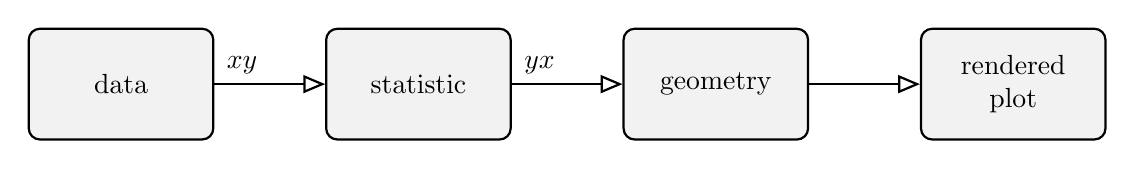
\begin{tikzpicture}[auto]
    \node [b] (data) {data};
    \node [b, right = of data] (statistic) {statistic};
    \node [b, right = of statistic] (geometry) {geometry};
    \node [b, right = of geometry] (render) {rendered\\plot};

    \path [ll] (statistic) -- (data) node[near end,above]{$x \rightleftarrows y$};
    \path [ll] (geometry) -- (statistic) node[near end,above]{$y \rightleftarrows x$};
    \path [ll] (render) -- (geometry) node[near end,above]{};
  \end{tikzpicture}}}\vspace{2ex}

In geometries, passing {orientation = "y"} results in flipping of the aesthetics but with a twist. For example, in \gggeom{geom\_line()}, flipping changes the drawing of the lines. Normally observations are sorted along the $x$ axis for drawing the segments connecting them. If we flip this layer, observations are sorted along the $y$ axis before drawing the connecting segments, which can make a major difference. The variables shown on each axis remain the same, as does the position of points drawn with \gggeom{geom\_point()}. In this example only two segments are the same in the flipped plot and the not-flipped one.

\begin{knitrout}\footnotesize
\definecolor{shadecolor}{rgb}{0.969, 0.969, 0.969}\color{fgcolor}\begin{kframe}
\begin{alltt}
\hlkwd{ggplot}\hlstd{(mtcars[}\hlnum{1}\hlopt{:}\hlnum{8}\hlstd{, ],} \hlkwd{aes}\hlstd{(}\hlkwc{x} \hlstd{= hp,} \hlkwc{y} \hlstd{= mpg))} \hlopt{+}
    \hlkwd{geom_point}\hlstd{()} \hlopt{+}
    \hlkwd{geom_line}\hlstd{(}\hlkwc{alpha} \hlstd{=} \hlnum{0.5}\hlstd{)} \hlopt{+}
    \hlkwd{geom_line}\hlstd{(}\hlkwc{alpha} \hlstd{=} \hlnum{0.5}\hlstd{,} \hlkwc{orientation} \hlstd{=} \hlstr{"y"}\hlstd{,} \hlkwc{colour} \hlstd{=} \hlstr{"red"}\hlstd{)}
\end{alltt}
\end{kframe}

{\centering \includegraphics[width=.54\textwidth]{figure/pos-flipping_box-01-ggplot-1} 

}


\end{knitrout}

\end{explainbox}

The next pair of examples exemplify automatic flipping using \ggstat{stat\_boxplot()}. Here we map the factor \code{Species} first to $x$ and then to $y$. In both cases boxplots have been computed and plotted for each level of the factor. Statistics \ggstat{stat\_boxplot()}, \ggstat{stat\_summary()}, \ggstat{stat\_histogram()} and \ggstat{stat\_density()} behave similarly with respect to flipping.

\begin{knitrout}\footnotesize
\definecolor{shadecolor}{rgb}{0.969, 0.969, 0.969}\color{fgcolor}\begin{kframe}
\begin{alltt}
\hlkwd{ggplot}\hlstd{(iris,} \hlkwd{aes}\hlstd{(}\hlkwc{x} \hlstd{= Species,} \hlkwc{y} \hlstd{= Sepal.Length))} \hlopt{+}
    \hlkwd{stat_boxplot}\hlstd{()}
\end{alltt}
\end{kframe}

{\centering \includegraphics[width=.54\textwidth]{figure/pos-flipping-01-ggplot-1} 

}


\end{knitrout}

\begin{knitrout}\footnotesize
\definecolor{shadecolor}{rgb}{0.969, 0.969, 0.969}\color{fgcolor}\begin{kframe}
\begin{alltt}
\hlkwd{ggplot}\hlstd{(iris,} \hlkwd{aes}\hlstd{(}\hlkwc{x} \hlstd{= Sepal.Length,} \hlkwc{y} \hlstd{= Species))} \hlopt{+}
    \hlkwd{stat_boxplot}\hlstd{()}
\end{alltt}
\end{kframe}

{\centering \includegraphics[width=.54\textwidth]{figure/pos-flipping-02-ggplot-1} 

}


\end{knitrout}

When we map a variable to only one of $x$ or $y$ the flip is also automatic.

\begin{knitrout}\footnotesize
\definecolor{shadecolor}{rgb}{0.969, 0.969, 0.969}\color{fgcolor}\begin{kframe}
\begin{alltt}
\hlkwd{ggplot}\hlstd{(iris,} \hlkwd{aes}\hlstd{(}\hlkwc{x} \hlstd{= Sepal.Length,} \hlkwc{color} \hlstd{= Species))} \hlopt{+}
    \hlkwd{stat_density}\hlstd{(}\hlkwc{fill} \hlstd{=} \hlnum{NA}\hlstd{)}
\end{alltt}
\end{kframe}

{\centering \includegraphics[width=.54\textwidth]{figure/pos-flipping-03-ggplot-1} 

}


\end{knitrout}

\begin{knitrout}\footnotesize
\definecolor{shadecolor}{rgb}{0.969, 0.969, 0.969}\color{fgcolor}\begin{kframe}
\begin{alltt}
\hlkwd{ggplot}\hlstd{(iris,} \hlkwd{aes}\hlstd{(}\hlkwc{y} \hlstd{= Sepal.Length,} \hlkwc{color} \hlstd{= Species))} \hlopt{+}
    \hlkwd{stat_density}\hlstd{(}\hlkwc{fill} \hlstd{=} \hlnum{NA}\hlstd{)}
\end{alltt}
\end{kframe}

{\centering \includegraphics[width=.54\textwidth]{figure/pos-flipping-04-ggplot-1} 

}


\end{knitrout}

\begin{explainbox}
In the case of ordinary least squares (OLS), regressions of $y$ on $x$ and of $x$ on $y$ in most cases yield different fitted lines, even if $R^2$ is consistent. This is due to the  assumption that $x$ values are known, either set or measured without error, i.e., not subject to random variation. All unexplained variation in the data is assumed to be in $y$. See Chapter \ref{chap:R:case:fitted:models} on page \pageref{chap:R:case:fitted:models} or consult a Statistics book such as \citetitle{Holmes2019} \autocite[][pp.\ 168--170]{Holmes2019} for additional information.
\end{explainbox}

With two continuous variables mapped, the default is to take $x$ as independent and $y$ as dependent. This matters, of course, when computations as in model fitting treat $x$ and $y$ differently. In this case parameter \code{orientation} can be used to indicate which of $x$ or $y$ is the independent or explanatory variable.



\begin{knitrout}\footnotesize
\definecolor{shadecolor}{rgb}{0.969, 0.969, 0.969}\color{fgcolor}\begin{kframe}
\begin{alltt}
\hlkwd{ggplot}\hlstd{(iris,} \hlkwd{aes}\hlstd{(Sepal.Length, Petal.Length))} \hlopt{+}
  \hlkwd{stat_smooth}\hlstd{(}\hlkwc{method} \hlstd{=} \hlstr{"lm"}\hlstd{,} \hlkwc{formula} \hlstd{= y} \hlopt{~} \hlstd{x)} \hlopt{+}
  \hlkwd{geom_point}\hlstd{()} \hlopt{+}
  \hlkwd{facet_wrap}\hlstd{(}\hlopt{~}\hlstd{Species,} \hlkwc{scales} \hlstd{=} \hlstr{"free"}\hlstd{)}
\end{alltt}
\end{kframe}

{\centering \includegraphics[width=.9\textwidth]{figure/pos-flipping-05-ggplot-1} 

}


\end{knitrout}

With \code{orientation = "y"} we tell that $y$ is the independent variable. In the case of \gggeom{geom\_smooth()} this means implicitly swapping $x$ and $y$ in \code{formula}.

\begin{knitrout}\footnotesize
\definecolor{shadecolor}{rgb}{0.969, 0.969, 0.969}\color{fgcolor}\begin{kframe}
\begin{alltt}
\hlkwd{ggplot}\hlstd{(iris,} \hlkwd{aes}\hlstd{(Sepal.Length, Petal.Length))} \hlopt{+}
    \hlkwd{stat_smooth}\hlstd{(}\hlkwc{method} \hlstd{=} \hlstr{"lm"}\hlstd{,} \hlkwc{formula} \hlstd{= y} \hlopt{~} \hlstd{x,} \hlkwc{orientation} \hlstd{=} \hlstr{"y"}\hlstd{)} \hlopt{+}
    \hlkwd{geom_point}\hlstd{()} \hlopt{+}
    \hlkwd{facet_wrap}\hlstd{(}\hlopt{~}\hlstd{Species,} \hlkwc{scales} \hlstd{=} \hlstr{"free"}\hlstd{)}
\end{alltt}
\end{kframe}

{\centering \includegraphics[width=.9\textwidth]{figure/pos-flipping-06-ggplot-1} 

}


\end{knitrout}

\begin{explainbox}
Flipping the orientation of plot layers with \code{orientation = "y"} is not equivalent to flipping the whole plot with \ggcoordinate{coord\_flip()}. In the first case which axis is considered independent for computation changes but not the positions of the axes in the plot, while in the second case the position of the $x$ and $y$ axes in the plot is swapped. So, when coordinates are flipped the $x$ aesthetic is plotted on the vertical axis and the $y$ aesthetic on the horizontal axis, but the role of the variable mapped to the \code{x} aesthetic remains as explanatory variable.

\begin{knitrout}\footnotesize
\definecolor{shadecolor}{rgb}{0.969, 0.969, 0.969}\color{fgcolor}\begin{kframe}
\begin{alltt}
\hlkwd{ggplot}\hlstd{(iris,} \hlkwd{aes}\hlstd{(Sepal.Length, Petal.Length))} \hlopt{+}
    \hlkwd{stat_smooth}\hlstd{(}\hlkwc{method} \hlstd{=} \hlstr{"lm"}\hlstd{,} \hlkwc{formula} \hlstd{= y} \hlopt{~} \hlstd{x)} \hlopt{+}
    \hlkwd{geom_point}\hlstd{()} \hlopt{+}
    \hlkwd{coord_flip}\hlstd{()} \hlopt{+}
    \hlkwd{facet_wrap}\hlstd{(}\hlopt{~}\hlstd{Species,} \hlkwc{scales} \hlstd{=} \hlstr{"free"}\hlstd{)}
\end{alltt}
\end{kframe}

{\centering \includegraphics[width=.9\textwidth]{figure/pos-flipping-06a-ggplot-1} 

}


\end{knitrout}
\end{explainbox}

In package \pkgname{ggpmisc} (version $\geq$ 0.4.1) statistics related to model fitting have an \code{orientation} parameter as those from package \ggplot do, but in addition they accept formulas where $x$ is on the lhs and $y$ on the rhs, such as \code{formula = x \~{} y} providing a syntax consistent with \Rlang's model fitting functions. In the next pair of examples we use \ggstat{stat\_poly\_line()}. In the first example in this pair, the default \code{formula = y \~{} x} is used, while in the second example we pass explicitly \code{formula = x \~{} y} to force the flipping of the fitted model. To make the difference clear, we plot both linear regressions on the same plots.

\begin{knitrout}\footnotesize
\definecolor{shadecolor}{rgb}{0.969, 0.969, 0.969}\color{fgcolor}\begin{kframe}
\begin{alltt}
\hlkwd{ggplot}\hlstd{(iris,} \hlkwd{aes}\hlstd{(Sepal.Length, Petal.Length))} \hlopt{+}
    \hlkwd{stat_poly_line}\hlstd{()} \hlopt{+}
    \hlkwd{stat_poly_line}\hlstd{(}\hlkwc{formula} \hlstd{= x} \hlopt{~} \hlstd{y,} \hlkwc{color} \hlstd{=} \hlstr{"red"}\hlstd{,} \hlkwc{fill} \hlstd{=} \hlstr{"yellow"}\hlstd{)} \hlopt{+}
    \hlkwd{geom_point}\hlstd{()} \hlopt{+}
    \hlkwd{facet_wrap}\hlstd{(}\hlopt{~}\hlstd{Species,} \hlkwc{scales} \hlstd{=} \hlstr{"free"}\hlstd{)}
\end{alltt}
\end{kframe}

{\centering \includegraphics[width=.9\textwidth]{figure/pos-flipping-07-ggpmisc-1} 

}


\end{knitrout}

In\index{plots!major axis regression}\label{par:ma:example} the case of the \code{iris} data used for these examples, both approaches used above to linear regression are wrong. The variables mapped to $x$ and$y$ are correlated but both are measured with error and subject to biological variation. In this case the correct approach is to not assume that there is a variable that can be considered independent, and instead use a method like major axis (MA) regression, as can be seen below.

\begin{knitrout}\footnotesize
\definecolor{shadecolor}{rgb}{0.969, 0.969, 0.969}\color{fgcolor}\begin{kframe}
\begin{alltt}
\hlkwd{ggplot}\hlstd{(iris,} \hlkwd{aes}\hlstd{(Sepal.Length, Petal.Length))} \hlopt{+}
    \hlkwd{stat_ma_line}\hlstd{()} \hlopt{+}
    \hlkwd{geom_point}\hlstd{()} \hlopt{+}
    \hlkwd{facet_wrap}\hlstd{(}\hlopt{~}\hlstd{Species,} \hlkwc{scales} \hlstd{=} \hlstr{"free"}\hlstd{)}
\end{alltt}
\end{kframe}

{\centering \includegraphics[width=.9\textwidth]{figure/pos-flipping-08-ggpmisc-1} 

}


\end{knitrout}

A related problem is when we need to summarize in the same plot layer $x$ and $y$ values. A simple example is adding a point with coordinates given by the means along the $x$ and $y$ axes as we need to pass these computed means simultaneously to \gggeom{geom\_point()}. Package \ggplot provides \ggstat{stat\_density\_2d()} and \ggstat{stat\_summary\_2d()}. However, \ggstat{stat\_summary\_2d()} uses bins, and is similar to \ggstat{stat\_density\_2d()} in how the computed values are returned. Package \pkgname{ggpmisc} provides two dimensional equivalents of \ggstat{stat\_summary()}: \ggstat{stat\_centroid()}, which applies the same summary function along $x$ and $y$, and \ggstat{stat\_summary\_xy()}, which accepts one function for $x$ and one for $y$.

\begin{knitrout}\footnotesize
\definecolor{shadecolor}{rgb}{0.969, 0.969, 0.969}\color{fgcolor}\begin{kframe}
\begin{alltt}
\hlkwd{ggplot}\hlstd{(iris,} \hlkwd{aes}\hlstd{(Sepal.Length, Petal.Length))} \hlopt{+}
    \hlkwd{geom_point}\hlstd{()} \hlopt{+}
    \hlkwd{stat_centroid}\hlstd{(}\hlkwc{color} \hlstd{=} \hlstr{"red"}\hlstd{)} \hlopt{+}
    \hlkwd{facet_wrap}\hlstd{(}\hlopt{~}\hlstd{Species,} \hlkwc{scales} \hlstd{=} \hlstr{"free"}\hlstd{)}
\end{alltt}
\end{kframe}

{\centering \includegraphics[width=.9\textwidth]{figure/pos-flipping-09-ggpmisc-1} 

}


\end{knitrout}

\begin{knitrout}\footnotesize
\definecolor{shadecolor}{rgb}{0.969, 0.969, 0.969}\color{fgcolor}\begin{kframe}
\begin{alltt}
\hlkwd{ggplot}\hlstd{(iris,} \hlkwd{aes}\hlstd{(Sepal.Length, Petal.Length))} \hlopt{+}
    \hlkwd{geom_point}\hlstd{()} \hlopt{+}
    \hlkwd{stat_centroid}\hlstd{(}\hlkwc{geom} \hlstd{=} \hlstr{"rug"}\hlstd{,} \hlkwc{sides} \hlstd{=} \hlstr{"trbl"}\hlstd{,}
                  \hlkwc{color} \hlstd{=} \hlstr{"red"}\hlstd{,} \hlkwc{size} \hlstd{=} \hlnum{1.5}\hlstd{)} \hlopt{+}
    \hlkwd{facet_wrap}\hlstd{(}\hlopt{~}\hlstd{Species,} \hlkwc{scales} \hlstd{=} \hlstr{"free"}\hlstd{)}
\end{alltt}
\end{kframe}

{\centering \includegraphics[width=.9\textwidth]{figure/pos-flipping-10-ggpmisc-1} 

}


\end{knitrout}

\begin{playground}
Which of the plots in the last two chunks above can be created by adding two layers with \ggstat{stat\_summary()}? Recreate this plot using \ggstat{stat\_summary()}.
\end{playground}

\index{grammar of graphics!flipped axes)}



\section{Facets}\label{sec:plot:facets}
\index{grammar of graphics!facets|(}
\index{plots!trellis-like}\index{plots!coordinated panels}
Facets are used in a special kind of plots containing multiple panels in which the panels share some properties.
These sets of coordinated panels are a useful tool for visualizing complex data. These plots became popular through the \code{trellis} graphs in \langname{S}, and the \pkgname{lattice} package in \Rlang. The basic idea is to have rows and/or columns of plots with common scales, all plots showing values for the same response variable. This is useful when there are multiple classification factors in a data set. Similar-looking plots, but with free scales or with the same scale but a `floating' intercept, are sometimes also useful. In \ggplot there are two possible types of facets: facets organized in a grid, and facets along a single `axis' of variation but, possibly, wrapped into two or more rows. These are produced by adding \Rfunction{facet\_grid()} or \Rfunction{facet\_wrap()}, respectively. In the examples below we use \gggeom{geom\_point()} but faceting can be used with \code{ggplot} objects containing diverse kinds of layers, displaying either observations or summaries from \code{data}.



We start by creating and saving a single-panel plot that we will use through this section to demonstrate how the same plot changes when we add facets.

\begin{knitrout}\footnotesize
\definecolor{shadecolor}{rgb}{0.969, 0.969, 0.969}\color{fgcolor}\begin{kframe}
\begin{alltt}
\hlstd{p} \hlkwb{<-} \hlkwd{ggplot}\hlstd{(}\hlkwc{data} \hlstd{= mtcars,} \hlkwd{aes}\hlstd{(wt, mpg))} \hlopt{+}
  \hlkwd{geom_point}\hlstd{()}
\hlstd{p}
\end{alltt}
\end{kframe}

{\centering \includegraphics[width=.7\textwidth]{figure/pos-facets-00-1} 

}


\end{knitrout}

A grid of panels has two dimensions, \code{rows} and \code{cols}. These dimensions in the grid of plot panels can be ``mapped'' to factors. Until recently a formula syntax was the only available one. Although this notation has been retained, the preferred syntax is currently to use the parameters \code{rows} and \code{cols}. We use \code{cols} in this example. Note that we need to use \code{vars()} to enclose the names of the variables in the data. The ``headings'' of the panels or \emph{strip labels} are by default the levels of the factors.

\begin{knitrout}\footnotesize
\definecolor{shadecolor}{rgb}{0.969, 0.969, 0.969}\color{fgcolor}\begin{kframe}
\begin{alltt}
\hlstd{p} \hlopt{+} \hlkwd{facet_grid}\hlstd{(}\hlkwc{cols} \hlstd{=} \hlkwd{vars}\hlstd{(cyl))}
\end{alltt}
\end{kframe}

{\centering \includegraphics[width=.7\textwidth]{figure/pos-facets-01-1} 

}


\end{knitrout}

In the ``historical notation'' the same plot would have been coded as follows.

\begin{knitrout}\footnotesize
\definecolor{shadecolor}{rgb}{0.969, 0.969, 0.969}\color{fgcolor}\begin{kframe}
\begin{alltt}
\hlstd{p} \hlopt{+} \hlkwd{facet_grid}\hlstd{(.} \hlopt{~} \hlstd{cyl)}
\end{alltt}
\end{kframe}
\end{knitrout}

By default, all panels share the same scale limits and share the plotting space evenly, but these defaults can be overridden.

\begin{knitrout}\footnotesize
\definecolor{shadecolor}{rgb}{0.969, 0.969, 0.969}\color{fgcolor}\begin{kframe}
\begin{alltt}
\hlstd{p} \hlopt{+} \hlkwd{facet_grid}\hlstd{(}\hlkwc{cols} \hlstd{=} \hlkwd{vars}\hlstd{(cyl),} \hlkwc{scales} \hlstd{=} \hlstr{"free"}\hlstd{)}
\hlstd{p} \hlopt{+} \hlkwd{facet_grid}\hlstd{(}\hlkwc{cols} \hlstd{=} \hlkwd{vars}\hlstd{(cyl),} \hlkwc{scales} \hlstd{=} \hlstr{"free"}\hlstd{,} \hlkwc{space} \hlstd{=} \hlstr{"free"}\hlstd{)}
\end{alltt}
\end{kframe}
\end{knitrout}



To obtain a 2D grid we need to specify both \code{rows} and \code{cols}.

\begin{knitrout}\footnotesize
\definecolor{shadecolor}{rgb}{0.969, 0.969, 0.969}\color{fgcolor}\begin{kframe}
\begin{alltt}
\hlstd{p} \hlopt{+} \hlkwd{facet_grid}\hlstd{(}\hlkwc{rows} \hlstd{=} \hlkwd{vars}\hlstd{(vs),} \hlkwc{cols} \hlstd{=} \hlkwd{vars}\hlstd{(am))}
\end{alltt}
\end{kframe}
\end{knitrout}



Margins display an additional column or row of panels with the combined data.

\begin{knitrout}\footnotesize
\definecolor{shadecolor}{rgb}{0.969, 0.969, 0.969}\color{fgcolor}\begin{kframe}
\begin{alltt}
\hlstd{p} \hlopt{+} \hlkwd{facet_grid}\hlstd{(}\hlkwc{cols} \hlstd{=} \hlkwd{vars}\hlstd{(cyl),} \hlkwc{margins} \hlstd{=} \hlnum{TRUE}\hlstd{)}
\end{alltt}
\end{kframe}

{\centering \includegraphics[width=.7\textwidth]{figure/pos-facets-06-1} 

}


\end{knitrout}

We can represent more than one variable per dimension of the grid of plot panels. For this example, we also override the default \code{labeller} used for the panels with one that includes the name of the variable in addition to factor levels in the \emph{strip labels}.

\begin{knitrout}\footnotesize
\definecolor{shadecolor}{rgb}{0.969, 0.969, 0.969}\color{fgcolor}\begin{kframe}
\begin{alltt}
\hlstd{p} \hlopt{+} \hlkwd{facet_grid}\hlstd{(}\hlkwc{cols} \hlstd{=} \hlkwd{vars}\hlstd{(vs, am),} \hlkwc{labeller} \hlstd{= label_both)}
\end{alltt}
\end{kframe}

{\centering \includegraphics[width=.7\textwidth]{figure/pos-facets-07-1} 

}


\end{knitrout}

\begin{explainbox}
Sometimes we may want to have mathematical expressions or Greek letters in the panel headings. The next example shows a way of achieving this. The key is to use as \code{labeller} a function that parses character strings into \Rlang expressions.

\begin{knitrout}\footnotesize
\definecolor{shadecolor}{rgb}{0.969, 0.969, 0.969}\color{fgcolor}\begin{kframe}
\begin{alltt}
\hlstd{mtcars}\hlopt{$}\hlstd{cyl12} \hlkwb{<-} \hlkwd{factor}\hlstd{(mtcars}\hlopt{$}\hlstd{cyl,}
                       \hlkwc{labels} \hlstd{=} \hlkwd{c}\hlstd{(}\hlstr{"alpha"}\hlstd{,} \hlstr{"beta"}\hlstd{,} \hlstr{"sqrt(x, y)"}\hlstd{))}
\hlstd{p1} \hlkwb{<-} \hlkwd{ggplot}\hlstd{(}\hlkwc{data} \hlstd{= mtcars,} \hlkwd{aes}\hlstd{(mpg, wt))} \hlopt{+}
      \hlkwd{geom_point}\hlstd{()} \hlopt{+}
      \hlkwd{facet_grid}\hlstd{(}\hlkwc{cols} \hlstd{=} \hlkwd{vars}\hlstd{(cyl12),} \hlkwc{labeller} \hlstd{= label_parsed)}
\end{alltt}
\end{kframe}
\end{knitrout}

More frequently we may need to include the levels of the factor used in the faceting as part of the labels. Here we use as \code{labeller}, function \Rfunction{label\_bquote()} with a special syntax that allows us to use an expression where replacement based on the facet (panel) data takes place. See section \ref{sec:plot:plotmath} for an example of the use of \code{bquote()}, the \Rlang function on which \Rfunction{label\_bquote()}, is built.



\begin{knitrout}\footnotesize
\definecolor{shadecolor}{rgb}{0.969, 0.969, 0.969}\color{fgcolor}\begin{kframe}
\begin{alltt}
\hlstd{p} \hlopt{+}
  \hlkwd{facet_grid}\hlstd{(}\hlkwc{cols} \hlstd{=} \hlkwd{vars}\hlstd{(cyl),}
             \hlkwc{labeller} \hlstd{=} \hlkwd{label_bquote}\hlstd{(}\hlkwc{cols} \hlstd{=} \hlkwd{.}\hlstd{(cyl)}\hlopt{~}\hlstr{"cylinders"}\hlstd{))}
\end{alltt}
\end{kframe}
\end{knitrout}

\end{explainbox}
%\begin{infobox}
%\sloppy
%In versions of \ggplot before 2.0.0, \code{labeller} was not implemented for \Rfunction{facet\_wrap()}, it was only available for \Rfunction{facet\_grid()}.
%\end{infobox}

In the next example we create a plot with wrapped facets. In this case the number of levels is small, and no wrapping takes place by default. In cases when more panels are present, wrapping into two or more continuation rows is the default. Here, we force wrapping with \code{nrow = 2}. When using \Rfunction{facet\_wrap()} there is only one dimension, and the parameter is called \code{facets}, instead of \code{rows} or \code{cols}.



\begin{knitrout}\footnotesize
\definecolor{shadecolor}{rgb}{0.969, 0.969, 0.969}\color{fgcolor}\begin{kframe}
\begin{alltt}
\hlstd{p} \hlopt{+} \hlkwd{facet_wrap}\hlstd{(}\hlkwc{facets} \hlstd{=} \hlkwd{vars}\hlstd{(cyl),} \hlkwc{nrow} \hlstd{=} \hlnum{2}\hlstd{)}
\end{alltt}
\end{kframe}

{\centering \includegraphics[width=.54\textwidth]{figure/pos-facets-13-1} 

}


\end{knitrout}

The example below (plot not shown), is similar to the earlier one for \code{facet\_grid}, but faceting according to two factors with \code{facet\_wrap()} along a single wrapped row of panels.

\begin{knitrout}\footnotesize
\definecolor{shadecolor}{rgb}{0.969, 0.969, 0.969}\color{fgcolor}\begin{kframe}
\begin{alltt}
\hlstd{p} \hlopt{+} \hlkwd{facet_wrap}\hlstd{(}\hlkwc{facets} \hlstd{=} \hlkwd{vars}\hlstd{(vs, am),} \hlkwc{nrow} \hlstd{=} \hlnum{2}\hlstd{,} \hlkwc{labeller} \hlstd{= label_both)}
\end{alltt}
\end{kframe}
\end{knitrout}


%In versions of \ggplot before 2.0.0, \code{labeller} was not implemented for
%\code{facet\_wrap()}, it was only available for \code{facet\_grid()}. In the current
%version it is implemented for both.
%
%<<echo=FALSE>>=
%opts_chunk$set(opts_fig_wide)
%@
%
%<<>>=
%p + facet_wrap(~ vs, labeller = label_bquote(alpha ^ .(vs)))
%@
\index{grammar of graphics!facets|)}

\section{Scales}\label{sec:plot:scales}
\index{grammar of graphics!scales|(}

In earlier sections of this chapter, examples have used the default \emph{scales} or we have set them with convenience functions. In the present section we describe in more detail the use of \emph{scales}. There are \emph{scales} available for different \emph{aesthetics} ($\approx$ attributes) of the plotted geometrical objects, such as position (\code{x, y, z}), \code{size}, \code{shape}, \code{linetype}, \code{color}, \code{fill}, \code{alpha} or transparency, \code{angle}. Scales determine how values in \code{data} are mapped to values of an \emph{aesthetics}, and how these values are labeled.

Depending on the characteristics of the data being mapped, \emph{scales} can be continuous or discrete, for \code{numeric} or \code{factor} variables in \code{data}, respectively. On the other hand, some \emph{aesthetics}, like \code{size}, can vary continuously but others like \code{linetype} are inherently discrete. In addition to discrete scales for inherently discrete \emph{aesthetics}, discrete scales are available for those \emph{aesthetics} that are inherently continuous, like \code{x}, \code{y}, \code{size}, \code{color}, etc.\

The scales used by default set the mapping automatically (e.g.,  which color value corresponds to $x = 0$ and which one to $x = 1$). However, for each \emph{aesthetic} such as \code{color}, there are multiple scales to choose from when creating a plot, both continuous and discrete (e.g.,  20 different color scales in \ggplot 3.2.0).

\begin{explainbox}
\emph{Aesthetics} in a plot layer, in addition to being determined by mappings, can also be set to constant values (e.g.,  plotting all points in a layer in red instead of the default black). \emph{Aesthetics} set to constant values, are not mapped to data, and are consequently independent of scales. In other words, properties of plot elements can be either set to a single constant value of an \emph{aesthetic} affecting all observations present in the layer \code{data}, or mapped to a variable in \code{data} in which case the value of the \emph{aesthetic}, such as \code{color}, will depend on the values of the mapped variable.
\end{explainbox}

The most direct mapping to data is \code{identity}, which means that the data is taken at its face value. In a color scale, say \ggscale{scale\_color\_identity()}, the variable in the data would be encoded with values such as \code{"red"}, \code{"blue"}---i.e., valid \Rlang colours. In a simple mapping using \ggscale{scale\_color\_discrete()} levels of a factor, such as \code{"treatment"} and \code{"control"} would be represented as distinct colours with the correspondence of individual factor levels to individual colours selected automatically by default. In contrast with \code{scale\_color\_manual()} the user needs to explicitly provide the mapping between factor levels and colours by passing arguments to the scale functions' parameters \code{breaks} and \code{values}.

A continuous data variable needs to be mapped to an \emph{aesthetic} through a continuous scale such as \code{scale\_color\_continuous()} or one its various variants. Values in a \code{numeric} variable will be mapped into a continuous range of colours, determined either automatically through a palette or manually by giving the colours at the extremes, and optionally at multiple intermediate values, within the range of variation of the mapped variable (e.g.,  scale settings so that the color varies gradually between \code{"red"} and \code{"gray50"}). Handling of missing values is such that mapping a value in a variable to an \code{NA} value for an aesthetic such as color makes the mapped values invisible. The reverse, mapping \code{NA} values in the data to a specific value of an aesthetic is also possible (e.g.,  displaying \code{NA} values in the mapped variable in red, while other values are mapped to shades of blue).

%
%
%\sloppy
%Advanced scale manipulation requires package \code{scales} to be loaded, although \ggplot (2.0.0 and later) re-export several functions from package \code{scales}. Some simple examples follow.

%\begin{infobox}
\subsection{Axis and key labels}\label{sec:plot:scale:name}\label{sec:plot:labs}
\index{plots!labels|(}
\index{plots!title|(}
\index{plots!subtitle|(}
\index{plots!tag|(}
\index{plots!caption|(}
First we describe a feature common to all scales, their \code{name}. The default \code{name} of all scales is the name of the variable or the expression mapped to it. In the case of the \code{x}, \code{y} and \code{z} \emph{aesthetics} the \code{name} given to the scale is used for the axis labels. For other \emph{aesthetics} the name of the scale becomes the ``heading'' or \emph{key title} of the guide or key. All scales have a \code{name} parameter to which a character string or \Rlang expression (see section \ref{sec:plot:plotmath}) can be passed as an argument to override the default.

Whole-plot title, subtitle and caption are not connected to \emph{scales} or \code{data}. A title (\code{label}) and \code{subtitle} can be added least confusingly with function \Rfunction{ggtitle()} by passing either character strings or \Rlang expressions as arguments.

\begin{knitrout}\footnotesize
\definecolor{shadecolor}{rgb}{0.969, 0.969, 0.969}\color{fgcolor}\begin{kframe}
\begin{alltt}
\hlkwd{ggplot}\hlstd{(}\hlkwc{data} \hlstd{= Orange,}
       \hlkwd{aes}\hlstd{(}\hlkwc{x} \hlstd{= age,} \hlkwc{y} \hlstd{= circumference,} \hlkwc{color} \hlstd{= Tree))} \hlopt{+}
  \hlkwd{geom_line}\hlstd{()} \hlopt{+}
  \hlkwd{geom_point}\hlstd{()} \hlopt{+}
  \hlkwd{expand_limits}\hlstd{(}\hlkwc{y} \hlstd{=} \hlnum{0}\hlstd{)} \hlopt{+}
  \hlkwd{scale_x_continuous}\hlstd{(}\hlkwc{name} \hlstd{=} \hlstr{"Time (d)"}\hlstd{)} \hlopt{+}
  \hlkwd{scale_y_continuous}\hlstd{(}\hlkwc{name} \hlstd{=} \hlstr{"Circumference (mm)"}\hlstd{)} \hlopt{+}
  \hlkwd{ggtitle}\hlstd{(}\hlkwc{label} \hlstd{=} \hlstr{"Growth of orange trees"}\hlstd{,}
          \hlkwc{subtitle} \hlstd{=} \hlstr{"Starting from 1968-12-31"}\hlstd{)}
\end{alltt}
\end{kframe}

{\centering \includegraphics[width=.7\textwidth]{figure/pos-axis-labels-01-1} 

}


\end{knitrout}

Convenience functions \Rfunction{xlab()} and \Rfunction{ylab()} can be used to set the axis labels to match those in the previous chunk.

\begin{knitrout}\footnotesize
\definecolor{shadecolor}{rgb}{0.969, 0.969, 0.969}\color{fgcolor}\begin{kframe}
\begin{alltt}
  \hlkwd{xlab}(\hlstr{"\hlkwd{Time} (d)"}) +
  \hlkwd{ylab}(\hlstr{"\hlkwd{Circumference} (mm)"}) +
\end{alltt}
\end{kframe}
\end{knitrout}

Convenience function \Rfunction{labs()} is useful when we use default scales for all the \emph{aesthetics} in a plot but want to manually set axis labels and/or key titles---i.e., the \code{name} of these scales. \Rfunction{labs()} accepts arguments for these names using, as parameter names, the names of the \emph{aesthetics}. It also allows us to set \code{title}, \code{subtitle}, \code{caption} and \code{tag}, of which the first two can also be set with \Rfunction{ggtitle()}.

\begin{knitrout}\footnotesize
\definecolor{shadecolor}{rgb}{0.969, 0.969, 0.969}\color{fgcolor}\begin{kframe}
\begin{alltt}
\hlkwd{ggplot}\hlstd{(}\hlkwc{data} \hlstd{= Orange,}
       \hlkwd{aes}\hlstd{(}\hlkwc{x} \hlstd{= age,} \hlkwc{y} \hlstd{= circumference,} \hlkwc{color} \hlstd{= Tree))} \hlopt{+}
  \hlkwd{geom_line}\hlstd{()} \hlopt{+}
  \hlkwd{geom_point}\hlstd{()} \hlopt{+}
  \hlkwd{expand_limits}\hlstd{(}\hlkwc{y} \hlstd{=} \hlnum{0}\hlstd{)} \hlopt{+}
  \hlkwd{labs}\hlstd{(}\hlkwc{title} \hlstd{=} \hlstr{"Growth of orange trees"}\hlstd{,}
       \hlkwc{subtitle} \hlstd{=} \hlstr{"Starting from 1968-12-31"}\hlstd{,}
       \hlkwc{caption} \hlstd{=} \hlstr{"see Draper, N. R. and Smith, H. (1998)"}\hlstd{,}
       \hlkwc{tag} \hlstd{=} \hlstr{"A"}\hlstd{,}
       \hlkwc{x} \hlstd{=} \hlstr{"Time (d)"}\hlstd{,}
       \hlkwc{y} \hlstd{=} \hlstr{"Circumference (mm)"}\hlstd{,}
       \hlkwc{color} \hlstd{=} \hlstr{"Tree\textbackslash{}nnumber"}\hlstd{)}
\end{alltt}
\end{kframe}

{\centering \includegraphics[width=.7\textwidth]{figure/pos-axis-labels-03-1} 

}


\end{knitrout}

\begin{playground}
Make an empty plot (\code{ggplot()}) and add to it as title an \Rlang expression producing $y = b_0 + b_1 x + b_2 x^2$. (Hint: have a look at the examples for the use of expressions in the \code{plotmath} demo in \Rlang by typing \code{demo(plotmath)} at the \Rlang console.
\end{playground}

%\begin{warningbox}
%Check!!
%When setting or updating labels using either \Rfunction{labs()} or \Rfunction{update\_labels()} be aware that even though \code{color} and \code{color} are synonyms for the same \emph{aesthetics}, the `name' used in the call to \Rfunction{aes()} must match the  `name' used when setting or updating the labels.
%\end{warningbox}
%
%The labels used in keys and axis tick-labels for factor levels can be changed through the different \emph{scales} as described in section \ref{sec:plot:scales} on page \pageref{sec:plot:scales}.
%
\index{plots!tag|)}
\index{plots!caption|)}
\index{plots!subtitle|)}
\index{plots!title|)}
\index{plots!labels|)}

\subsection{Continuous scales}\label{sec:plot:scales:continuous}
\index{grammar of graphics!continuous scales|(}
We start by listing the most frequently used arguments to the continuous scale functions: \code{name}, \code{breaks}, \code{minor\_breaks}, \code{labels}, \code{limits}, \code{expand}, \code{na.value}, \code{trans}, \code{guide}, and \code{position}. The value of \code{name} is used for axis labels or the key title (see previous section). The arguments to \code{breaks} and \code{minor\_breaks} override the default locations of major and minor ticks and grid lines. Setting them to \code{NULL} suppresses the ticks. By default the tick labels are generated from the value of \code{breaks} but an argument to \code{labels} of the same length as \code{breaks} will replace these defaults. The values of \code{limits} determine both the range of values in the data included and the plotting area as described above---by default the out-of-bounds (\code{oob}) observations are replaced by \code{NA} but it is possible to instead ``squish'' these observations towards the edge of the plotting area. The argument to \code{expand} determines the size of the margins or padding added to the area delimited by \code{lims} when setting the ``visual'' plotting area. The value passed to \code{na.value} is used as a replacement for \code{NA} valued observations---most useful for \code{color} and \code{fill} aesthetics. The transformation object passed as an argument to \code{trans} determines the transformation used---the transformation affects the rendering, but breaks and tick labels remain expressed in the original data units. The argument to \code{guide} determines the type of key or removes the default key. Depending on the scale in question not all these parameters are available.



We generate new fake data.

\begin{knitrout}\footnotesize
\definecolor{shadecolor}{rgb}{0.969, 0.969, 0.969}\color{fgcolor}\begin{kframe}
\begin{alltt}
\hlstd{fake2.data} \hlkwb{<-}
  \hlkwd{data.frame}\hlstd{(}\hlkwc{y} \hlstd{=} \hlkwd{c}\hlstd{(}\hlkwd{rnorm}\hlstd{(}\hlnum{20}\hlstd{,} \hlkwc{mean} \hlstd{=} \hlnum{20}\hlstd{,} \hlkwc{sd} \hlstd{=} \hlnum{5}\hlstd{),}
                   \hlkwd{rnorm}\hlstd{(}\hlnum{20}\hlstd{,} \hlkwc{mean} \hlstd{=} \hlnum{40}\hlstd{,} \hlkwc{sd} \hlstd{=} \hlnum{10}\hlstd{)),}
             \hlkwc{group} \hlstd{=} \hlkwd{factor}\hlstd{(}\hlkwd{c}\hlstd{(}\hlkwd{rep}\hlstd{(}\hlstr{"A"}\hlstd{,} \hlnum{20}\hlstd{),} \hlkwd{rep}\hlstd{(}\hlstr{"B"}\hlstd{,} \hlnum{20}\hlstd{))),}
             \hlkwc{z} \hlstd{=} \hlkwd{rnorm}\hlstd{(}\hlnum{40}\hlstd{,} \hlkwc{mean} \hlstd{=} \hlnum{12}\hlstd{,} \hlkwc{sd} \hlstd{=} \hlnum{6}\hlstd{))}
\end{alltt}
\end{kframe}
\end{knitrout}
\subsubsection{Limits}

Limits are relevant to all kinds of \emph{scales}. Limits are set through parameter \code{limits} of the different scale functions. They can also be set with convenience functions \code{xlim()} and \code{ylim()} in the case of the \code{x} and \code{y} \emph{aesthetics}, and more generally with function \code{lims()} which like \code{labs()}, takes arguments named according to the name of the \emph{aesthetics}. The \code{limits} argument of scales accepts vectors, factors or a function computing them from \code{data}. In contrast, the convenience functions do not accept functions as their arguments.

In the next example we set ``hard'' limits, which will exclude some observations from the plot and from any computation of summaries or fitting of smoothers. More exactly, the off-limits observations are converted to \code{NA} values before they are passed as \code{data} to \emph{geometries}.

\begin{knitrout}\footnotesize
\definecolor{shadecolor}{rgb}{0.969, 0.969, 0.969}\color{fgcolor}\begin{kframe}
\begin{alltt}
\hlkwd{ggplot}\hlstd{(fake2.data,} \hlkwd{aes}\hlstd{(z, y))} \hlopt{+} \hlkwd{geom_point}\hlstd{()} \hlopt{+}
  \hlkwd{scale_y_continuous}\hlstd{(}\hlkwc{limits} \hlstd{=} \hlkwd{c}\hlstd{(}\hlnum{0}\hlstd{,} \hlnum{100}\hlstd{))}
\end{alltt}
\end{kframe}
\end{knitrout}

To set only one limit leaving the other free, we can use \code{NA} as a boundary.

\begin{knitrout}\footnotesize
\definecolor{shadecolor}{rgb}{0.969, 0.969, 0.969}\color{fgcolor}\begin{kframe}
\begin{alltt}
  \hlkwd{scale_y_continuous}\hlstd{(}\hlkwc{limits} \hlstd{=} \hlkwd{c}\hlstd{(}\hlnum{50}\hlstd{,} \hlnum{NA}\hlstd{))}
\end{alltt}
\end{kframe}
\end{knitrout}

Convenience functions \Rfunction{ylim()} and \Rfunction{xlim()} can be used to set the limits to the default $x$ and $y$ scales in use. We here use \Rfunction{ylim()}, but \Rfunction{xlim()} is identical except for the \emph{scale} it affects.

\begin{knitrout}\footnotesize
\definecolor{shadecolor}{rgb}{0.969, 0.969, 0.969}\color{fgcolor}\begin{kframe}
\begin{alltt}
  \hlkwd{ylim}\hlstd{(}\hlnum{50}\hlstd{,} \hlnum{NA}\hlstd{)}
\end{alltt}
\end{kframe}
\end{knitrout}

In general, setting hard limits should be avoided, even though a warning is issued about \code{NA} values being omitted, as it is easy to unwillingly subset the data being plotted.
It is preferable to use function \Rfunction{expand\_limits()} as it safely \emph{expands} the dynamically computed default limits of a scale---the scale limits will grow past the requested expanded limits when needed to accommodate all observations. The arguments to \code{x} and \code{y} are numeric vectors of length one or two each, matching how the limits of the $x$ and $y$ continuous scales are defined. Here we expand the limits to include the origin.

\begin{knitrout}\footnotesize
\definecolor{shadecolor}{rgb}{0.969, 0.969, 0.969}\color{fgcolor}\begin{kframe}
\begin{alltt}
\hlkwd{ggplot}\hlstd{(fake2.data,} \hlkwd{aes}\hlstd{(z, y))} \hlopt{+}
  \hlkwd{geom_point}\hlstd{()} \hlopt{+}
  \hlkwd{expand_limits}\hlstd{(}\hlkwc{y} \hlstd{=} \hlnum{0}\hlstd{,} \hlkwc{x} \hlstd{=} \hlnum{0}\hlstd{)}
\end{alltt}
\end{kframe}

{\centering \includegraphics[width=.54\textwidth]{figure/pos-scale-limits-04-1} 

}


\end{knitrout}

The \code{expand} parameter of the scales plays a different role than \Rfunction{expand\_limits()}. It controls how much larger the ``visual'' plotting area is compared to the limits of the actual plotting area. In other words, it adds a ``margin'' or padding to the plotting area outside the limits set either dynamically or manually. Very rarely plots are drawn so that observations are plotted on top of the axes, avoiding this is a key role of \code{expand}. Rug plots and marginal annotations will also require the plotting area to be expanded. In \ggplot the default is to always apply some expansion.

We here set the upper limit of the plotting area to be expanded by adding padding to the top and remove the default padding from the bottom of the plotting area.

\begin{knitrout}\footnotesize
\definecolor{shadecolor}{rgb}{0.969, 0.969, 0.969}\color{fgcolor}\begin{kframe}
\begin{alltt}
\hlkwd{ggplot}\hlstd{(fake2.data,}
  \hlkwd{aes}\hlstd{(}\hlkwc{fill} \hlstd{= group,} \hlkwc{color} \hlstd{= group,} \hlkwc{x} \hlstd{= y))} \hlopt{+}
  \hlkwd{stat_density}\hlstd{(}\hlkwc{alpha} \hlstd{=} \hlnum{0.3}\hlstd{)} \hlopt{+}
  \hlkwd{scale_y_continuous}\hlstd{(}\hlkwc{expand} \hlstd{=} \hlkwd{expand_scale}\hlstd{(}\hlkwc{add} \hlstd{=} \hlkwd{c}\hlstd{(}\hlnum{0}\hlstd{,} \hlnum{0.02}\hlstd{)))}
\end{alltt}
\end{kframe}
\end{knitrout}

Here we instead use a multiplier to a similar effect as above; we add 10\% compared to the range of the \code{limits}.

\begin{knitrout}\footnotesize
\definecolor{shadecolor}{rgb}{0.969, 0.969, 0.969}\color{fgcolor}\begin{kframe}
\begin{alltt}
  \hlkwd{scale_y_continuous}\hlstd{(}\hlkwc{expand} \hlstd{=} \hlkwd{expand_scale}\hlstd{(}\hlkwc{mult} \hlstd{=} \hlkwd{c}\hlstd{(}\hlnum{0}\hlstd{,} \hlnum{0.1}\hlstd{)))}
\end{alltt}
\end{kframe}
\end{knitrout}

In the case of scales, we cannot reverse their direction through the setting of limits. We need instead to use a transformation as described in section \ref{sec:plot:scales:trans} on page \pageref{sec:plot:scales:trans}. But, inconsistently, \Rfunction{xlim()} and \Rfunction{ylim()} do implicitly allow this transformation through the numeric values passed as limits.

%%% to be moved
%We can also use \code{limits} with discrete scales, listing all or some of the levels of a factor that are to be included in the scale. This works even if the levels are defined in the factor but not present in a given data set, such as after subsetting.

\begin{playground}
Test what the result is when the first limit is larger than the second one. Is it the same as when setting these same values as limits with \code{ylim()}?

\begin{knitrout}\footnotesize
\definecolor{shadecolor}{rgb}{0.969, 0.969, 0.969}\color{fgcolor}\begin{kframe}
\begin{alltt}
\hlkwd{ggplot}\hlstd{(fake2.data,} \hlkwd{aes}\hlstd{(z, y))} \hlopt{+} \hlkwd{geom_point}\hlstd{()} \hlopt{+}
  \hlkwd{scale_y_continuous}\hlstd{(}\hlkwc{limits} \hlstd{=} \hlkwd{c}\hlstd{(}\hlnum{100}\hlstd{,} \hlnum{0}\hlstd{))}
\end{alltt}
\end{kframe}
\end{knitrout}
\end{playground}

\subsubsection{Ticks and their labels}\label{sec:plot:scales:ticks}

Parameter \code{breaks}\index{plots!scales!tick breaks} is used to set the location of ticks along the axis. Parameter \code{labels}\index{plots!scales!tick labels} is used to set the tick labels. Both parameters can be passed either a vector or a function as an argument. The default is to compute ``good'' breaks based on the limits and format the numbers as strings.

When manually setting breaks, we can keep the default computed labels for the \code{breaks}.

\begin{knitrout}\footnotesize
\definecolor{shadecolor}{rgb}{0.969, 0.969, 0.969}\color{fgcolor}\begin{kframe}
\begin{alltt}
\hlkwd{ggplot}\hlstd{(fake2.data,} \hlkwd{aes}\hlstd{(z, y))} \hlopt{+}
  \hlkwd{geom_point}\hlstd{()} \hlopt{+}
  \hlkwd{scale_y_continuous}\hlstd{(}\hlkwc{breaks} \hlstd{=} \hlkwd{c}\hlstd{(}\hlnum{20}\hlstd{, pi} \hlopt{*} \hlnum{10}\hlstd{,} \hlnum{40}\hlstd{,} \hlnum{60}\hlstd{))}
\end{alltt}
\end{kframe}
\end{knitrout}

The default breaks are computed by function \Rfunction{pretty\_breaks()} from \pkgname{scales}. The argument passed to its parameter \code{n} determines the target number ticks to be generated automatically, but the actual number of ticks computed may be slightly different depending on the range of the data.

\begin{knitrout}\footnotesize
\definecolor{shadecolor}{rgb}{0.969, 0.969, 0.969}\color{fgcolor}\begin{kframe}
\begin{alltt}
  \hlkwd{scale_y_continuous}\hlstd{(}\hlkwc{breaks} \hlstd{=} \hlkwd{pretty_breaks}\hlstd{(}\hlkwc{n} \hlstd{=} \hlnum{7}\hlstd{))}
\end{alltt}
\end{kframe}
\end{knitrout}

We can set tick labels manually, in parallel to the setting of \code{breaks} by passing as arguments two vectors of equal length. In the next example we use an expression to obtain a Greek letter.

\begin{knitrout}\footnotesize
\definecolor{shadecolor}{rgb}{0.969, 0.969, 0.969}\color{fgcolor}\begin{kframe}
\begin{alltt}
\hlkwd{ggplot}\hlstd{(fake2.data,} \hlkwd{aes}\hlstd{(z, y))} \hlopt{+}
  \hlkwd{geom_point}\hlstd{()} \hlopt{+}
  \hlkwd{scale_y_continuous}\hlstd{(}\hlkwc{breaks} \hlstd{=} \hlkwd{c}\hlstd{(}\hlnum{20}\hlstd{, pi} \hlopt{*} \hlnum{10}\hlstd{,} \hlnum{40}\hlstd{,} \hlnum{60}\hlstd{),}
                     \hlkwc{labels} \hlstd{=} \hlkwd{c}\hlstd{(}\hlstr{"20"}\hlstd{,} \hlkwd{expression}\hlstd{(}\hlnum{10}\hlopt{*}\hlstd{pi),} \hlstr{"40"}\hlstd{,} \hlstr{"60"}\hlstd{))}
\end{alltt}
\end{kframe}

{\centering \includegraphics[width=.54\textwidth]{figure/pos-scale-ticks-02-1} 

}


\end{knitrout}

Package \pkgname{scales} provides several functions for the automatic generation of tick labels. For example, to display tick labels as percentages for data available as decimal fractions, we can use function \code{percent()}.

\begin{knitrout}\footnotesize
\definecolor{shadecolor}{rgb}{0.969, 0.969, 0.969}\color{fgcolor}\begin{kframe}
\begin{alltt}
\hlkwd{ggplot}\hlstd{(fake2.data,} \hlkwd{aes}\hlstd{(z, y} \hlopt{/} \hlkwd{max}\hlstd{(y)))} \hlopt{+}
  \hlkwd{geom_point}\hlstd{()} \hlopt{+}
  \hlkwd{scale_y_continuous}\hlstd{(}\hlkwc{labels} \hlstd{= percent)}
\end{alltt}
\end{kframe}

{\centering \includegraphics[width=.54\textwidth]{figure/pos-scale-ticks-03-1} 

}


\end{knitrout}

For currency, we can use \code{dollar()}, to include commas separating thousands, millions, so on, we can use \code{comma()}, and for numbers formatted using exponents of 10---useful for logarithmic-transformed scales---we can use \code{scientific\_format()}, \code{label\_number(scale\_cut = cut\_short\_scale())}, \code{label\_log()}, or \code{label\_number(scale\_cut = cut\_si("g")}. As shown below, some of these functions can be useful with untransformed continuous scales.

\begin{knitrout}\footnotesize
\definecolor{shadecolor}{rgb}{0.969, 0.969, 0.969}\color{fgcolor}\begin{kframe}
\begin{alltt}
\hlkwd{ggplot}\hlstd{(fake2.data,} \hlkwd{aes}\hlstd{(z, y} \hlopt{*} \hlnum{1000}\hlstd{))} \hlopt{+}
  \hlkwd{geom_point}\hlstd{()} \hlopt{+}
  \hlkwd{scale_y_continuous}\hlstd{(}\hlkwc{name} \hlstd{=} \hlstr{"Mass"}\hlstd{,} \hlkwc{labels} \hlstd{=} \hlkwd{label_number}\hlstd{(}\hlkwc{scale_cut} \hlstd{=} \hlkwd{cut_si}\hlstd{(}\hlstr{"g"}\hlstd{)))}
\end{alltt}
\end{kframe}

{\centering \includegraphics[width=.54\textwidth]{figure/pos-scale-ticks-04-1} 

}


\end{knitrout}

With date values mapped to $x$ or $y$, tick labels are created with functions \Rfunction{label\_date()} or \Rfunction{label\_date\_short()}. In the case of time, tick labels are created with function \Rfunction{label\_time()}.

\begin{knitrout}\footnotesize
\definecolor{shadecolor}{rgb}{0.969, 0.969, 0.969}\color{fgcolor}\begin{kframe}
\begin{alltt}
\hlcom{## ADD EXAMPLES USING FORMATS for dates and times}
\end{alltt}
\end{kframe}
\end{knitrout}

It is also possible to use user-defined functions both for breaks and labels.

\subsubsection{Transformed scales}\label{sec:plot:scales:trans}

The\index{plots!scales!transformations} default scales used by the \code{x} and \code{y} aesthetics, \ggscale{scale\_x\_continuous()} and \ggscale{scale\_y\_continuous()}, accept a user-supplied transformation function as an argument to \code{trans} with default code{trans = "identity"} (no transformation). In addition, there are predefined convenience scale functions for \code{log10}, \code{sqrt} and \code{reverse}.

\begin{warningbox}
  Similar to the maths functions of \Rlang, the name of the scales are \ggscale{scale\_x\_log10()} and \ggscale{scale\_y\_log10()} rather than \ggscale{scale\_y\_log()} because in \Rlang, the function \code{log} returns the natural logarithm.
\end{warningbox}

We can use \ggscale{scale\_x\_reverse()} to reverse the direction of a continuous scale,

\begin{knitrout}\footnotesize
\definecolor{shadecolor}{rgb}{0.969, 0.969, 0.969}\color{fgcolor}\begin{kframe}
\begin{alltt}
\hlkwd{ggplot}\hlstd{(fake2.data,} \hlkwd{aes}\hlstd{(z, y))} \hlopt{+}
  \hlkwd{geom_point}\hlstd{()} \hlopt{+}
  \hlkwd{scale_x_reverse}\hlstd{()}
\end{alltt}
\end{kframe}

{\centering \includegraphics[width=.54\textwidth]{figure/pos-scale-trans-01-1} 

}


\end{knitrout}

Axis tick-labels display the original values before applying the transformation. The \code{"breaks"} need to be given in the original scale as well. We use \ggscale{scale\_y\_log10()} to apply a $\log_{10}$ transformation to the $y$ values.

\begin{knitrout}\footnotesize
\definecolor{shadecolor}{rgb}{0.969, 0.969, 0.969}\color{fgcolor}\begin{kframe}
\begin{alltt}
  \hlkwd{scale_y_log10}\hlstd{(}\hlkwc{breaks}\hlstd{=}\hlkwd{c}\hlstd{(}\hlnum{10}\hlstd{,}\hlnum{20}\hlstd{,}\hlnum{50}\hlstd{,}\hlnum{100}\hlstd{))}
\end{alltt}
\end{kframe}
\end{knitrout}

Using a transformation in a scale is not equivalent to applying the same transformation on the fly when mapping a variable to the $x$  (or $y$) \emph{aesthetic} as this results in tick-labels expressed in transformed values.

\begin{knitrout}\footnotesize
\definecolor{shadecolor}{rgb}{0.969, 0.969, 0.969}\color{fgcolor}\begin{kframe}
\begin{alltt}
\hlkwd{ggplot}\hlstd{(fake2.data,} \hlkwd{aes}\hlstd{(z,} \hlkwd{log10}\hlstd{(y)))} \hlopt{+}
  \hlkwd{geom_point}\hlstd{()}
\end{alltt}
\end{kframe}
\end{knitrout}

We show next how to specify a transformation to a continuous scale, using a predefined ``transformation'' object.

\begin{knitrout}\footnotesize
\definecolor{shadecolor}{rgb}{0.969, 0.969, 0.969}\color{fgcolor}\begin{kframe}
\begin{alltt}
  \hlkwd{scale_y_continuous}\hlstd{(}\hlkwc{trans} \hlstd{=} \hlstr{"reciprocal"}\hlstd{)}
\end{alltt}
\end{kframe}
\end{knitrout}

Natural logarithms are important in growth analysis as the slope against time gives the relative growth rate. We show this with the \code{Orange} data set.

\begin{knitrout}\footnotesize
\definecolor{shadecolor}{rgb}{0.969, 0.969, 0.969}\color{fgcolor}\begin{kframe}
\begin{alltt}
\hlkwd{ggplot}\hlstd{(}\hlkwc{data} \hlstd{= Orange,}
       \hlkwd{aes}\hlstd{(}\hlkwc{x} \hlstd{= age,} \hlkwc{y} \hlstd{= circumference,} \hlkwc{color} \hlstd{= Tree))} \hlopt{+}
  \hlkwd{geom_line}\hlstd{()} \hlopt{+}
  \hlkwd{geom_point}\hlstd{()} \hlopt{+}
  \hlkwd{scale_y_continuous}\hlstd{(}\hlkwc{trans} \hlstd{=} \hlstr{"log"}\hlstd{,} \hlkwc{breaks} \hlstd{=} \hlkwd{c}\hlstd{(}\hlnum{20}\hlstd{,} \hlnum{50}\hlstd{,} \hlnum{100}\hlstd{,} \hlnum{200}\hlstd{))}
\end{alltt}
\end{kframe}
\end{knitrout}

\subsubsection{Position of $x$ and $y$ axes}
\index{plots!axis position}

The default position of axes can be changed through parameter \code{position}, using character constants \code{"bottom"}, \code{"top"}, \code{"left"} and \code{"right"}.

\begin{knitrout}\footnotesize
\definecolor{shadecolor}{rgb}{0.969, 0.969, 0.969}\color{fgcolor}\begin{kframe}
\begin{alltt}
\hlkwd{ggplot}\hlstd{(}\hlkwc{data} \hlstd{= mtcars,} \hlkwd{aes}\hlstd{(wt, mpg))} \hlopt{+}
  \hlkwd{geom_point}\hlstd{()} \hlopt{+}
  \hlkwd{scale_x_continuous}\hlstd{(}\hlkwc{position} \hlstd{=} \hlstr{"top"}\hlstd{)} \hlopt{+}
  \hlkwd{scale_y_continuous}\hlstd{(}\hlkwc{position} \hlstd{=} \hlstr{"right"}\hlstd{)}
\end{alltt}
\end{kframe}

{\centering \includegraphics[width=.54\textwidth]{figure/pos-axis-position-01-1} 

}


\end{knitrout}

\subsubsection{Secondary axes}

It\index{plots!secondary axes} is also possible to add secondary axes with ticks displayed in a transformed scale.

\begin{knitrout}\footnotesize
\definecolor{shadecolor}{rgb}{0.969, 0.969, 0.969}\color{fgcolor}\begin{kframe}
\begin{alltt}
\hlkwd{ggplot}\hlstd{(}\hlkwc{data} \hlstd{= mtcars,} \hlkwd{aes}\hlstd{(wt, mpg))} \hlopt{+}
  \hlkwd{geom_point}\hlstd{()} \hlopt{+}
  \hlkwd{scale_y_continuous}\hlstd{(}\hlkwc{sec.axis} \hlstd{=} \hlkwd{sec_axis}\hlstd{(}\hlopt{~} \hlstd{.} \hlopt{^-}\hlnum{1}\hlstd{,} \hlkwc{name} \hlstd{=} \hlstr{"1/y"}\hlstd{) )}
\end{alltt}
\end{kframe}

{\centering \includegraphics[width=.54\textwidth]{figure/pos-axis-secondary-01-1} 

}


\end{knitrout}

It is also possible to use different \code{breaks} and \code{labels} than for the main axes, and to provide a different \code{name} to be used as a secondary axis label.

\begin{knitrout}\footnotesize
\definecolor{shadecolor}{rgb}{0.969, 0.969, 0.969}\color{fgcolor}\begin{kframe}
\begin{alltt}
  \hlkwd{scale_y_continuous}\hlstd{(}\hlkwc{sec.axis} \hlstd{=} \hlkwd{sec_axis}\hlstd{(}\hlopt{~} \hlstd{.} \hlopt{/} \hlnum{2.3521458}\hlstd{,} \hlkwc{name} \hlstd{=} \hlkwd{expression}\hlstd{(km} \hlopt{/} \hlstd{l),}
                                         \hlkwc{breaks} \hlstd{=} \hlkwd{c}\hlstd{(}\hlnum{5}\hlstd{,} \hlnum{7.5}\hlstd{,} \hlnum{10}\hlstd{,} \hlnum{12.5}\hlstd{)))}
\end{alltt}
\end{kframe}
\end{knitrout}
\index{grammar of graphics!continuous scales|)}

\subsection{Time and date scales for $x$ and $y$}\label{sec:plot:scales:time:date}
\index{grammar of graphics!time and date scales|(}
In \Rlang and many other computing languages, time values are stored as integer or numeric values subject to special interpretation. Times stored as objects of class \code{POSIXct} can be mapped to continuous \emph{aesthetics} such as $x$ and $y$. Special scales are available for these quantities.

We can set limits and breaks using constants as time or dates. These are most easily input with the functions in packages \pkgname{lubridate} or \pkgname{anytime}.


\begin{warningbox}
Warnings are issued in the next two chunks as we are using scale limits to subset a part of the observations present in \code{data}.
\end{warningbox}

\begin{knitrout}\footnotesize
\definecolor{shadecolor}{rgb}{0.969, 0.969, 0.969}\color{fgcolor}\begin{kframe}
\begin{alltt}
\hlkwd{ggplot}\hlstd{(}\hlkwc{data} \hlstd{= weather_wk_25_2019.tb,}
       \hlkwd{aes}\hlstd{(}\hlkwd{with_tz}\hlstd{(time,} \hlkwc{tzone} \hlstd{=} \hlstr{"EET"}\hlstd{), air_temp_C))} \hlopt{+}
  \hlkwd{geom_line}\hlstd{()} \hlopt{+}
  \hlkwd{scale_x_datetime}\hlstd{(}\hlkwc{name} \hlstd{=} \hlkwa{NULL}\hlstd{,}
                   \hlkwc{breaks} \hlstd{=} \hlkwd{ymd_hm}\hlstd{(}\hlstr{"2019-06-11 12:00"}\hlstd{,} \hlkwc{tz} \hlstd{=} \hlstr{"EET"}\hlstd{)} \hlopt{+} \hlkwd{days}\hlstd{(}\hlnum{0}\hlopt{:}\hlnum{1}\hlstd{),}
                   \hlkwc{limits} \hlstd{=} \hlkwd{ymd_hm}\hlstd{(}\hlstr{"2019-06-11 00:00"}\hlstd{,} \hlkwc{tz} \hlstd{=} \hlstr{"EET"}\hlstd{)} \hlopt{+} \hlkwd{days}\hlstd{(}\hlkwd{c}\hlstd{(}\hlnum{0}\hlstd{,} \hlnum{2}\hlstd{)))} \hlopt{+}
  \hlkwd{scale_y_continuous}\hlstd{(}\hlkwc{name} \hlstd{=} \hlstr{"Air temperature (C)"}\hlstd{)} \hlopt{+}
  \hlkwd{expand_limits}\hlstd{(}\hlkwc{y} \hlstd{=} \hlnum{0}\hlstd{)}
\end{alltt}


{\ttfamily\noindent\color{warningcolor}{\#\# Warning: Removed 7199 rows containing missing values (`geom\_line()`).}}\end{kframe}

{\centering \includegraphics[width=.9\textwidth]{figure/pos-scale-datetime-01-1} 

}


\end{knitrout}

By\index{plots!scales!axis labels} default the tick labels produced and their formatting are automatically selected based on the extent of the time data. For example, if we have all data collected within a single day, then the tick labels will show hours and minutes. If we plot data for several years, the labels will show the date portion of the time instant. The default is frequently good enough, but it is possible, as for numbers, to use different formatter functions to generate the tick labels.

\begin{knitrout}\footnotesize
\definecolor{shadecolor}{rgb}{0.969, 0.969, 0.969}\color{fgcolor}\begin{kframe}
\begin{alltt}
\hlkwd{ggplot}\hlstd{(}\hlkwc{data} \hlstd{= weather_wk_25_2019.tb,}
       \hlkwd{aes}\hlstd{(}\hlkwd{with_tz}\hlstd{(time,} \hlkwc{tzone} \hlstd{=} \hlstr{"EET"}\hlstd{), air_temp_C))} \hlopt{+}
  \hlkwd{geom_line}\hlstd{()} \hlopt{+}
  \hlkwd{scale_x_datetime}\hlstd{(}\hlkwc{name} \hlstd{=} \hlkwa{NULL}\hlstd{,}
                   \hlkwc{date_breaks} \hlstd{=} \hlstr{"1 hour"}\hlstd{,}
                   \hlkwc{limits} \hlstd{=} \hlkwd{ymd_hm}\hlstd{(}\hlstr{"2019-06-16 00:00"}\hlstd{,} \hlkwc{tz} \hlstd{=} \hlstr{"EET"}\hlstd{)} \hlopt{+} \hlkwd{hours}\hlstd{(}\hlkwd{c}\hlstd{(}\hlnum{6}\hlstd{,} \hlnum{18}\hlstd{)),}
                   \hlkwc{date_labels} \hlstd{=} \hlstr{"%H:%M"}\hlstd{)} \hlopt{+}
  \hlkwd{scale_y_continuous}\hlstd{(}\hlkwc{name} \hlstd{=} \hlstr{"Air temperature (C)"}\hlstd{)} \hlopt{+}
  \hlkwd{expand_limits}\hlstd{(}\hlkwc{y} \hlstd{=} \hlnum{0}\hlstd{)}
\end{alltt}


{\ttfamily\noindent\color{warningcolor}{\#\# Warning: Removed 9359 rows containing missing values (`geom\_line()`).}}\end{kframe}

{\centering \includegraphics[width=.9\textwidth]{figure/pos-scale-datetime-02-1} 

}


\end{knitrout}

\begin{playground}
The formatting strings used are those supported by \Rfunction{strptime()} and \code{help(strptime)} lists them. Change, in the two examples above, the $y$-axis labels used and the limits---e.g., include a single hour or a whole week of data, check which tick labels are produced by default and then pass as an argument to \code{date\_labels} different format strings, taking into account that in addition to the \emph{conversion specification} codes, format strings can include additional text.
\end{playground}
\index{grammar of graphics!time and date scales|)}

\subsection{Discrete scales for $x$ and $y$}
\index{grammar of graphics!discrete scales|(}

In\index{plots!scales!limits} the case of ordered or unordered factors, the tick labels are by default the names of the factor levels. Consequently, one roundabout way of obtaining the desired tick labels is to set them as factor levels. This approach is not recommended as in many cases the text of the desired tick labels may not be recognized as a valid name making the code using them more difficult to type in scripts or at the command prompt. It is best to use simple mnemonic short names for factor levels and variables, and to set suitable labels through \emph{scales} when plotting, as we will show here.

We can use \ggscale{scale\_x\_discrete()} to reorder and select the columns without altering the data. If we use this approach to subset the data, then to avoid warnings we need to add \code{na.rm = TRUE}. We additionally use \code{scale\_x\_discrete} to convert level names to uppercase.


\begin{knitrout}\footnotesize
\definecolor{shadecolor}{rgb}{0.969, 0.969, 0.969}\color{fgcolor}\begin{kframe}
\begin{alltt}
\hlkwd{ggplot}\hlstd{(mpg,} \hlkwd{aes}\hlstd{(class, hwy))} \hlopt{+}
  \hlkwd{stat_summary}\hlstd{(}\hlkwc{geom} \hlstd{=} \hlstr{"col"}\hlstd{,} \hlkwc{fun} \hlstd{= mean,} \hlkwc{na.rm} \hlstd{=} \hlnum{TRUE}\hlstd{)} \hlopt{+}
  \hlkwd{scale_x_discrete}\hlstd{(}\hlkwc{limits} \hlstd{=} \hlkwd{c}\hlstd{(}\hlstr{"compact"}\hlstd{,} \hlstr{"subcompact"}\hlstd{,} \hlstr{"midsize"}\hlstd{),}
                   \hlkwc{labels} \hlstd{=} \hlkwd{c}\hlstd{(}\hlstr{"COMPACT"}\hlstd{,} \hlstr{"SUBCOMPACT"}\hlstd{,} \hlstr{"MIDSIZE"}\hlstd{))}
\end{alltt}
\end{kframe}

{\centering \includegraphics[width=.54\textwidth]{figure/pos-scale-discrete-10-1} 

}


\end{knitrout}

If, as in the previous example, only the case of character strings needs to be changed, passing function \Rfunction{toupper()} or \Rfunction{tolower()} allows a more general and less error-prone approach. In fact any function, user defined or not, which converts the values of \code{limits} into the desired values can be passed as an argument to \code{labels}.

\begin{knitrout}\footnotesize
\definecolor{shadecolor}{rgb}{0.969, 0.969, 0.969}\color{fgcolor}\begin{kframe}
\begin{alltt}
  \hlkwd{scale_x_discrete}\hlstd{(}\hlkwc{limits} \hlstd{=} \hlkwd{c}\hlstd{(}\hlstr{"compact"}\hlstd{,} \hlstr{"subcompact"}\hlstd{,} \hlstr{"midsize"}\hlstd{),}
                   \hlkwc{labels} \hlstd{= toupper)}
\end{alltt}
\end{kframe}
\end{knitrout}

Alternatively, we can change the order of the columns in the plot by reordering the levels of factor \code{mpg\$class}. This approach makes sense if the ordering needs to be done programmatically based on values in \code{data}. See section \ref{sec:calc:factors} on page \pageref{sec:calc:factors} for details. The example below shows how to reorder the columns, corresponding to the levels of \code{class} based on the \code{mean()} of \code{hwy}.

\begin{knitrout}\footnotesize
\definecolor{shadecolor}{rgb}{0.969, 0.969, 0.969}\color{fgcolor}\begin{kframe}
\begin{alltt}
\hlkwd{ggplot}\hlstd{(mpg,} \hlkwd{aes}\hlstd{(}\hlkwd{reorder}\hlstd{(}\hlkwc{x} \hlstd{=} \hlkwd{factor}\hlstd{(class),} \hlkwc{X} \hlstd{= hwy,} \hlkwc{FUN} \hlstd{= mean), hwy))} \hlopt{+}
  \hlkwd{stat_summary}\hlstd{(}\hlkwc{geom} \hlstd{=} \hlstr{"col"}\hlstd{,} \hlkwc{fun} \hlstd{= mean)}
\end{alltt}
\end{kframe}
\end{knitrout}
\index{grammar of graphics!discrete scales|)}


\subsection{Size}
\index{grammar of graphics!size scales|(}
For the \code{size} \emph{aesthetic}, several scales are available, both discrete and continuous. They do not differ much from those already described above. \emph{Geometries} \gggeom{geom\_point()}, \gggeom{geom\_line()}, \gggeom{geom\_hline()}, \gggeom{geom\_vline()}, \gggeom{geom\_text()}, \gggeom{geom\_label()} obey \code{size} as expected. In the case of \gggeom{geom\_bar()}, \gggeom{geom\_col()}, \gggeom{geom\_area()} and all other geometric elements bordered by lines, \code{size} is obeyed by these border lines. In fact, other aesthetics natural for lines such as \code{linetype} also apply to these borders.

When using \code{size} scales, \code{breaks} and \code{labels} affect the key or \code{guide}. In scales that produce a key passing \code{guide = "none"} removes the key corresponding to the scale.
\index{grammar of graphics!size scales|)}

\subsection{Color and fill}
\index{grammar of graphics!color and fill scales|(}
\index{plots!with colors|(}

color and fill scales are similar, but they affect different elements of the plot. All visual elements in a plot obey the \code{color} \emph{aesthetic}, but only elements that have an inner region and a boundary, obey both \code{color} and \code{fill} \emph{aesthetics}. There are separate but equivalent sets of scales available for these two \emph{aesthetics}. We will describe in more detail the \code{color} \emph{aesthetic} and give only some examples for \code{fill}. We will, however, start by reviewing how colors are defined and used in \Rlang.

\subsubsection{Color definitions in R}\label{sec:plot:colors}
\index{color!definitions|(}
Colors can be specified in \Rlang not only through character strings with the names of previously defined colors, but also directly as strings describing the RGB (red, green and blue) components as hexadecimal numbers (on base 16 expressed using 0, 1, 2, 3, 4, 6, 7, 8, 9, A, B, C, D, E, and F as ``digits'') such as \code{"\#FFFFFF"} for white or \code{"\#000000"} for black, or \code{"\#FF0000"} for the brightest available pure red.

The list of color names\index{color!names} known to \Rlang can be obtained be typing \code{colors()} at the \Rlang console.
Given the number of colors available, we may want to subset them based on their names. Function \code{colors()} returns a character vector. We can use \code{grep()} to find the names containing a given character substring, in this example \code{"dark"}.

\begin{knitrout}\footnotesize
\definecolor{shadecolor}{rgb}{0.969, 0.969, 0.969}\color{fgcolor}\begin{kframe}
\begin{alltt}
\hlkwd{length}\hlstd{(}\hlkwd{colors}\hlstd{())}
\end{alltt}
\begin{verbatim}
## [1] 657
\end{verbatim}
\begin{alltt}
\hlkwd{grep}\hlstd{(}\hlstr{"dark"}\hlstd{,}\hlkwd{colors}\hlstd{(),} \hlkwc{value} \hlstd{=} \hlnum{TRUE}\hlstd{)}
\end{alltt}
\begin{verbatim}
##  [1] "darkblue"        "darkcyan"        "darkgoldenrod"   "darkgoldenrod1" 
##  [5] "darkgoldenrod2"  "darkgoldenrod3"  "darkgoldenrod4"  "darkgray"       
##  [9] "darkgreen"       "darkgrey"        "darkkhaki"       "darkmagenta"    
## [13] "darkolivegreen"  "darkolivegreen1" "darkolivegreen2" "darkolivegreen3"
## [17] "darkolivegreen4" "darkorange"      "darkorange1"     "darkorange2"    
## [21] "darkorange3"     "darkorange4"     "darkorchid"      "darkorchid1"    
## [25] "darkorchid2"     "darkorchid3"     "darkorchid4"     "darkred"        
## [29] "darksalmon"      "darkseagreen"    "darkseagreen1"   "darkseagreen2"  
## [33] "darkseagreen3"   "darkseagreen4"   "darkslateblue"   "darkslategray"  
## [37] "darkslategray1"  "darkslategray2"  "darkslategray3"  "darkslategray4" 
## [41] "darkslategrey"   "darkturquoise"   "darkviolet"
\end{verbatim}
\end{kframe}
\end{knitrout}

To retrieve the RGB values for a color definition we use:

\begin{knitrout}\footnotesize
\definecolor{shadecolor}{rgb}{0.969, 0.969, 0.969}\color{fgcolor}\begin{kframe}
\begin{alltt}
\hlkwd{col2rgb}\hlstd{(}\hlstr{"purple"}\hlstd{)}
\end{alltt}
\begin{verbatim}
##       [,1]
## red    160
## green   32
## blue   240
\end{verbatim}
\begin{alltt}
\hlkwd{col2rgb}\hlstd{(}\hlstr{"#FF0000"}\hlstd{)}
\end{alltt}
\begin{verbatim}
##       [,1]
## red    255
## green    0
## blue     0
\end{verbatim}
\end{kframe}
\end{knitrout}

Color definitions in \Rlang can contain a \emph{transparency} described by an \code{alpha} value, which by default is not returned.

\begin{knitrout}\footnotesize
\definecolor{shadecolor}{rgb}{0.969, 0.969, 0.969}\color{fgcolor}\begin{kframe}
\begin{alltt}
\hlkwd{col2rgb}\hlstd{(}\hlstr{"purple"}\hlstd{,} \hlkwc{alpha} \hlstd{=} \hlnum{TRUE}\hlstd{)}
\end{alltt}
\begin{verbatim}
##       [,1]
## red    160
## green   32
## blue   240
## alpha  255
\end{verbatim}
\end{kframe}
\end{knitrout}

With function \Rfunction{rgb()} we can define new colors. Enter \code{help(rgb)} for more details.

\begin{knitrout}\footnotesize
\definecolor{shadecolor}{rgb}{0.969, 0.969, 0.969}\color{fgcolor}\begin{kframe}
\begin{alltt}
\hlkwd{rgb}\hlstd{(}\hlnum{1}\hlstd{,} \hlnum{1}\hlstd{,} \hlnum{0}\hlstd{)}
\end{alltt}
\begin{verbatim}
## [1] "#FFFF00"
\end{verbatim}
\begin{alltt}
\hlkwd{rgb}\hlstd{(}\hlnum{1}\hlstd{,} \hlnum{1}\hlstd{,} \hlnum{0}\hlstd{,} \hlkwc{names} \hlstd{=} \hlstr{"my.color"}\hlstd{)}
\end{alltt}
\begin{verbatim}
##  my.color 
## "#FFFF00"
\end{verbatim}
\begin{alltt}
\hlkwd{rgb}\hlstd{(}\hlnum{255}\hlstd{,} \hlnum{255}\hlstd{,} \hlnum{0}\hlstd{,} \hlkwc{names} \hlstd{=} \hlstr{"my.color"}\hlstd{,} \hlkwc{maxColorValue} \hlstd{=} \hlnum{255}\hlstd{)}
\end{alltt}
\begin{verbatim}
##  my.color 
## "#FFFF00"
\end{verbatim}
\end{kframe}
\end{knitrout}

As described above, colors can be defined in the RGB \emph{color space}, however, other color models such as HSV (hue, saturation, value) can be also used to define colours.

\begin{knitrout}\footnotesize
\definecolor{shadecolor}{rgb}{0.969, 0.969, 0.969}\color{fgcolor}\begin{kframe}
\begin{alltt}
\hlkwd{hsv}\hlstd{(}\hlkwd{c}\hlstd{(}\hlnum{0}\hlstd{,}\hlnum{0.25}\hlstd{,}\hlnum{0.5}\hlstd{,}\hlnum{0.75}\hlstd{,}\hlnum{1}\hlstd{),} \hlnum{0.5}\hlstd{,} \hlnum{0.5}\hlstd{)}
\end{alltt}
\begin{verbatim}
## [1] "#804040" "#608040" "#408080" "#604080" "#804040"
\end{verbatim}
\end{kframe}
\end{knitrout}

Probably a more useful flavor of HSV colors for use in scales are those returned by function \Rfunction{hcl()} for hue, chroma and luminance. While the ``value'' and ``saturation'' in HSV are based on physical values, the ``chroma'' and ``luminance'' values in HCL are based on human visual perception. Colours with equal luminance will be seen as equally bright by an ``average'' human. In a scale based on different hues but equal chroma and luminance values, as used by package \ggplot, all colours are perceived as equally bright. The hues need to be expressed as angles in degrees, with values between zero and 360.

\begin{knitrout}\footnotesize
\definecolor{shadecolor}{rgb}{0.969, 0.969, 0.969}\color{fgcolor}\begin{kframe}
\begin{alltt}
\hlkwd{hcl}\hlstd{(}\hlkwd{c}\hlstd{(}\hlnum{0}\hlstd{,}\hlnum{0.25}\hlstd{,}\hlnum{0.5}\hlstd{,}\hlnum{0.75}\hlstd{,}\hlnum{1}\hlstd{)} \hlopt{*} \hlnum{360}\hlstd{)}
\end{alltt}
\begin{verbatim}
## [1] "#FFC5D0" "#D4D8A7" "#99E2D8" "#D5D0FC" "#FFC5D0"
\end{verbatim}
\end{kframe}
\end{knitrout}

It is also important to remember that humans can only distinguish a limited set of colours, and even smaller color gamuts can be reproduced by screens and printers. Furthermore, variation from individual to individual exists in color perception, including different types of color blindness. It is important to take this into account when choosing the colors used in illustrations.
\index{color!definitions|)}

\subsection{Continuous color-related scales}
\sloppy
Continuous color scales \ggscale{scale\_color\_continuous()}, \ggscale{scale\_color\_gradient()}, \ggscale{scale\_color\_gradient2()},  \ggscale{scale\_color\_gradientn()}, \ggscale{scale\_color\_date()} and \ggscale{scale\_color\_datetime()}, give a smooth continuous gradient between two or more colours. They are used with \code{numeric}, \code{date} and \code{datetime} data. A corresponding set of \code{fill} scales is also available. Other scales like \ggscale{scale\_color\_viridis\_c()} and \ggscale{scale\_color\_distiller()} are based on the use of ready-made palettes of sets of color gradients chosen to work well together under multiple conditions or for human vision including different types of color blindness.

\subsection{Discrete color-related scales}
\sloppy
Color scales \ggscale{scale\_color\_discrete()}, \ggscale{scale\_color\_hue()}, \ggscale{scale\_color\_gray()} are used with categorical data stored as factors. Other scales like \ggscale{scale\_color\_viridis\_d()} and \ggscale{scale\_color\_brewer()} provide discrete sets of colours based on palettes.

\subsection{Binned scales}\label{sec:binned:scales}
\index{grammar of graphics!binned scales|(}
Before version 3.3.0 of \pkgname{ggplot2} only two types of scales were available, continuous and discrete. A third type of scales (implemented for all the aesthetics where relevant) was added in version 3.3.0 called \emph{binned}. They are to be used with continuous variables, but they discretize the continuous values into bins or classes, each for a range of values, and then represent them in the plot using a discrete set of values. We re-do the figure shown on page \pageref{chunk:plot:weighted:resid} but replacing \ggscale{scale\_color\_gradient()} by \ggscale{scale\_color\_binned()}.

\begin{knitrout}\footnotesize
\definecolor{shadecolor}{rgb}{0.969, 0.969, 0.969}\color{fgcolor}\begin{kframe}
\begin{alltt}
\hlcom{# we use capital letters X and Y as variable names to distinguish}
\hlcom{# them from the x and y aesthetics}
\hlkwd{set.seed}\hlstd{(}\hlnum{4321}\hlstd{)}
\hlstd{X} \hlkwb{<-} \hlnum{0}\hlopt{:}\hlnum{10}
\hlstd{Y} \hlkwb{<-} \hlstd{(X} \hlopt{+} \hlstd{X}\hlopt{^}\hlnum{2} \hlopt{+} \hlstd{X}\hlopt{^}\hlnum{3}\hlstd{)} \hlopt{+} \hlkwd{rnorm}\hlstd{(}\hlkwd{length}\hlstd{(X),} \hlkwc{mean} \hlstd{=} \hlnum{0}\hlstd{,} \hlkwc{sd} \hlstd{=} \hlkwd{mean}\hlstd{(X}\hlopt{^}\hlnum{3}\hlstd{)} \hlopt{/} \hlnum{4}\hlstd{)}
\hlstd{my.data} \hlkwb{<-} \hlkwd{data.frame}\hlstd{(X, Y)}
\hlstd{my.data.outlier} \hlkwb{<-} \hlstd{my.data}
\hlstd{my.data.outlier[}\hlnum{6}\hlstd{,} \hlstr{"Y"}\hlstd{]} \hlkwb{<-} \hlstd{my.data.outlier[}\hlnum{6}\hlstd{,} \hlstr{"Y"}\hlstd{]} \hlopt{*} \hlnum{10}
\end{alltt}
\end{kframe}
\end{knitrout}

\begin{knitrout}\footnotesize
\definecolor{shadecolor}{rgb}{0.969, 0.969, 0.969}\color{fgcolor}\begin{kframe}
\begin{alltt}
\hlstd{my.formula} \hlkwb{<-} \hlstd{y} \hlopt{~} \hlkwd{poly}\hlstd{(x,} \hlnum{3}\hlstd{,} \hlkwc{raw} \hlstd{=} \hlnum{TRUE}\hlstd{)}
\end{alltt}
\end{kframe}
\end{knitrout}

\begin{knitrout}\footnotesize
\definecolor{shadecolor}{rgb}{0.969, 0.969, 0.969}\color{fgcolor}\begin{kframe}
\begin{alltt}
\hlkwd{ggplot}\hlstd{(my.data.outlier)} \hlopt{+}
  \hlkwd{stat_fit_residuals}\hlstd{(}\hlkwc{formula} \hlstd{= my.formula,}
                     \hlkwc{method} \hlstd{=} \hlstr{"rlm"}\hlstd{,}
                     \hlkwc{mapping} \hlstd{=} \hlkwd{aes}\hlstd{(}\hlkwc{x} \hlstd{= X,}
                                   \hlkwc{y} \hlstd{=} \hlkwd{stage}\hlstd{(}\hlkwc{start} \hlstd{= Y,}
                                             \hlkwc{after_stat} \hlstd{= y} \hlopt{*} \hlstd{weights),}
                                   \hlkwc{colour} \hlstd{=} \hlkwd{after_stat}\hlstd{(weights)),}
                     \hlkwc{show.legend} \hlstd{=} \hlnum{TRUE}\hlstd{)} \hlopt{+}
  \hlkwd{scale_color_binned}\hlstd{(}\hlkwc{low} \hlstd{=} \hlstr{"red"}\hlstd{,} \hlkwc{high} \hlstd{=} \hlstr{"blue"}\hlstd{,} \hlkwc{limits} \hlstd{=} \hlkwd{c}\hlstd{(}\hlnum{0}\hlstd{,} \hlnum{1}\hlstd{),}
                     \hlkwc{guide} \hlstd{=} \hlstr{"colourbar"}\hlstd{,} \hlkwc{n.breaks} \hlstd{=} \hlnum{5}\hlstd{)}
\end{alltt}
\end{kframe}

{\centering \includegraphics[width=.7\textwidth]{figure/pos-binned-scales-01-1} 

}


\end{knitrout}

The advantage of binned scales is that they facilitate the fast reading of the plot while their disadvantage is the decreased resolution of the scale. The choice of a binned vs.\ continuous scale, and the number and boundaries of bins, set by the argument passed to parameter \code{n.breaks} or to \code{breaks} need to be chosen carefully, taking into account the audience, the length of time available to the viewer to peruse the plot vs.\ the density of observations. Transformations are also allowed in these scales as in others.

\index{grammar of graphics!binned scales|)}

\subsection{Identity scales}
\index{grammar of graphics!identity color scales|(}
In the case of identity scales, the mapping is one to-one to the data. For example, if we map the \code{color} or \code{fill} \emph{aesthetic} to a variable using \ggscale{scale\_color\_identity()} or \ggscale{scale\_fill\_identity()}, the mapped variable must already contain valid color definitions. In the case of mapping \code{alpha}, the variable must contain numeric values in the range 0 to 1.

We create a data frame containing a variable \code{colors} containing character strings interpretable as the names of color definitions known to \Rlang. We then use them directly in the plot.

\begin{knitrout}\footnotesize
\definecolor{shadecolor}{rgb}{0.969, 0.969, 0.969}\color{fgcolor}\begin{kframe}
\begin{alltt}
\hlstd{df99} \hlkwb{<-} \hlkwd{data.frame}\hlstd{(}\hlkwc{x} \hlstd{=} \hlnum{1}\hlopt{:}\hlnum{10}\hlstd{,} \hlkwc{y} \hlstd{=} \hlkwd{dnorm}\hlstd{(}\hlnum{10}\hlstd{),} \hlkwc{colors} \hlstd{=} \hlkwd{rep}\hlstd{(}\hlkwd{c}\hlstd{(}\hlstr{"red"}\hlstd{,} \hlstr{"blue"}\hlstd{),} \hlnum{5}\hlstd{))}

\hlkwd{ggplot}\hlstd{(df99,} \hlkwd{aes}\hlstd{(x, y,} \hlkwc{color} \hlstd{= colors))} \hlopt{+}
  \hlkwd{geom_point}\hlstd{()} \hlopt{+}
  \hlkwd{scale_color_identity}\hlstd{()}
\end{alltt}
\end{kframe}

{\centering \includegraphics[width=.7\textwidth]{figure/pos-scale-color-10-1} 

}


\end{knitrout}

\begin{playground}
How does the plot look, if the identity scale is deleted from the example above? Edit and re-run the example code.

While using the identity scale, how would you need to change the code example above, to produce a plot with green and purple points?
\end{playground}
\index{grammar of graphics!identity color scales|)}
\index{plots!with colors|)}
\index{grammar of graphics!color and fill scales|)}
\index{grammar of graphics!scales|)}

\section{Adding annotations}\label{sec:plot:annotations}
\index{grammar of graphics!annotations|(}
The idea of annotations is that they add plot elements that are not directly connected with \code{data}, which we could call ``decorations'' such as arrows used to highlight some feature of the data, specific points along an axis, etc. They are referenced to the ``natural'' coordinates used to plot the observations, but are elements that do not represent observations or summaries computed from the observations.  Annotations are added to a ggplot with \Rfunction{annotate()} as plot layers (each call to \code{annotate()} creates a new layer). To achieve the behavior expected of annotations, \Rfunction{annotate()} does not inherit the default \code{data} or \code{mapping} of variables to \emph{aesthetics}. Annotations frequently make use of \code{"text"} or \code{"label"} \emph{geometries} with character strings as data, possibly to be parsed as expressions. However, for example, the \code{"segment"} geometry can be used to add arrows.

\begin{warningbox}
While layers added to a plot directly using \emph{geometries} and \emph{statistics} respect faceting, annotation layers added with \Rfunction{annotate()} are replicated unchanged in every panel of a faceted plot. The reason is that annotation layers accept \emph{aesthetics} only as constant values which are the same for every panel as no grouping is possible without a \code{mapping} to \code{data}.
\end{warningbox}

We show a simple example using \code{"text"} as \emph{geometry}.

\begin{knitrout}\footnotesize
\definecolor{shadecolor}{rgb}{0.969, 0.969, 0.969}\color{fgcolor}\begin{kframe}
\begin{alltt}
\hlkwd{ggplot}\hlstd{(fake2.data,} \hlkwd{aes}\hlstd{(z, y))} \hlopt{+}
  \hlkwd{geom_point}\hlstd{()} \hlopt{+}
  \hlkwd{annotate}\hlstd{(}\hlkwc{geom} \hlstd{=} \hlstr{"text"}\hlstd{,}
           \hlkwc{label} \hlstd{=} \hlstr{"origin"}\hlstd{,}
           \hlkwc{x} \hlstd{=} \hlnum{0}\hlstd{,} \hlkwc{y} \hlstd{=} \hlnum{0}\hlstd{,}
           \hlkwc{color} \hlstd{=} \hlstr{"blue"}\hlstd{,}
           \hlkwc{size}\hlstd{=}\hlnum{4}\hlstd{)}
\end{alltt}
\end{kframe}

{\centering \includegraphics[width=.7\textwidth]{figure/pos-annotate-01-1} 

}


\end{knitrout}

\begin{playground}
Play with the values of the arguments to \Rfunction{annotate()} to vary the position, size, color, font family, font face, rotation angle and justification of the annotation.
\end{playground}

\index{plots!insets as annotations|(}
It is relatively common to use inset tables, plots, bitmaps or vector plots as annotations. With \Rfunction{annotation\_custom()}, grobs (\pkgname{grid} graphical object) can be added to a ggplot. To add another or the same plot as an inset, we first need to convert it into a grob. In the case of a ggplot we use \Rfunction{ggplotGrob()}. In this example the inset is a zoomed-in window into the main plot. In addition to the grob, we need to provide the coordinates expressed in ``natural'' data units of the main plot for the location of the grob.

\begin{knitrout}\footnotesize
\definecolor{shadecolor}{rgb}{0.969, 0.969, 0.969}\color{fgcolor}\begin{kframe}
\begin{alltt}
\hlstd{p} \hlkwb{<-} \hlkwd{ggplot}\hlstd{(fake2.data,} \hlkwd{aes}\hlstd{(z, y))} \hlopt{+}
  \hlkwd{geom_point}\hlstd{()}
\hlstd{p} \hlopt{+} \hlkwd{expand_limits}\hlstd{(}\hlkwc{x} \hlstd{=} \hlnum{40}\hlstd{)} \hlopt{+}
  \hlkwd{annotation_custom}\hlstd{(}\hlkwd{ggplotGrob}\hlstd{(p} \hlopt{+} \hlkwd{coord_cartesian}\hlstd{(}\hlkwc{xlim} \hlstd{=} \hlkwd{c}\hlstd{(}\hlnum{5}\hlstd{,} \hlnum{10}\hlstd{),} \hlkwc{ylim} \hlstd{=} \hlkwd{c}\hlstd{(}\hlnum{20}\hlstd{,} \hlnum{40}\hlstd{))} \hlopt{+}
                               \hlkwd{theme_bw}\hlstd{(}\hlnum{10}\hlstd{)),}
                    \hlkwc{xmin} \hlstd{=} \hlnum{21}\hlstd{,} \hlkwc{xmax} \hlstd{=} \hlnum{40}\hlstd{,} \hlkwc{ymin} \hlstd{=} \hlnum{30}\hlstd{,} \hlkwc{ymax} \hlstd{=} \hlnum{60}\hlstd{)}
\end{alltt}
\end{kframe}

{\centering \includegraphics[width=.7\textwidth]{figure/pos-inset-01-1} 

}


\end{knitrout}

This approach has the limitation that if used together with faceting, the inset will be the same for each plot panel. See section \ref{sec:plot:insets} on page \pageref{sec:plot:insets} for \emph{geometries} that can be used to add insets.
\index{plots!insets as annotations|)}

In the next example, in addition to adding expressions as annotations, we also pass expressions as tick labels through the scale. Do notice that we use recycling for setting the breaks, as \code{c(0, 0.5, 1, 1.5, 2) * pi} is equivalent to \code{c(0, 0.5 * pi, pi, 1.5 * pi, 2 * pi}. Annotations are plotted at their own position, unrelated to any observation in the data, but using the same coordinates and units as for plotting the data.

\begin{knitrout}\footnotesize
\definecolor{shadecolor}{rgb}{0.969, 0.969, 0.969}\color{fgcolor}\begin{kframe}
\begin{alltt}
\hlkwd{ggplot}\hlstd{(}\hlkwd{data.frame}\hlstd{(}\hlkwc{x} \hlstd{=} \hlkwd{c}\hlstd{(}\hlnum{0}\hlstd{,} \hlnum{2} \hlopt{*} \hlstd{pi)),} \hlkwd{aes}\hlstd{(}\hlkwc{x} \hlstd{= x))} \hlopt{+}
  \hlkwd{stat_function}\hlstd{(}\hlkwc{fun} \hlstd{= sin)} \hlopt{+}
  \hlkwd{scale_x_continuous}\hlstd{(}
    \hlkwc{breaks} \hlstd{=} \hlkwd{c}\hlstd{(}\hlnum{0}\hlstd{,} \hlnum{0.5}\hlstd{,} \hlnum{1}\hlstd{,} \hlnum{1.5}\hlstd{,} \hlnum{2}\hlstd{)} \hlopt{*} \hlstd{pi,}
    \hlkwc{labels} \hlstd{=} \hlkwd{c}\hlstd{(}\hlstr{"0"}\hlstd{,} \hlkwd{expression}\hlstd{(}\hlnum{0.5}\hlopt{~}\hlstd{pi),} \hlkwd{expression}\hlstd{(pi),}
             \hlkwd{expression}\hlstd{(}\hlnum{1.5}\hlopt{~}\hlstd{pi),} \hlkwd{expression}\hlstd{(}\hlnum{2}\hlopt{~}\hlstd{pi)))} \hlopt{+}
  \hlkwd{labs}\hlstd{(}\hlkwc{y} \hlstd{=} \hlstr{"sin(x)"}\hlstd{)} \hlopt{+}
  \hlkwd{annotate}\hlstd{(}\hlkwc{geom} \hlstd{=} \hlstr{"text"}\hlstd{,}
           \hlkwc{label} \hlstd{=} \hlkwd{c}\hlstd{(}\hlstr{"+"}\hlstd{,} \hlstr{"-"}\hlstd{),}
           \hlkwc{x} \hlstd{=} \hlkwd{c}\hlstd{(}\hlnum{0.5}\hlstd{,} \hlnum{1.5}\hlstd{)} \hlopt{*} \hlstd{pi,} \hlkwc{y} \hlstd{=} \hlkwd{c}\hlstd{(}\hlnum{0.5}\hlstd{,} \hlopt{-}\hlnum{0.5}\hlstd{),}
           \hlkwc{size} \hlstd{=} \hlnum{20}\hlstd{)} \hlopt{+}
  \hlkwd{annotate}\hlstd{(}\hlkwc{geom} \hlstd{=} \hlstr{"point"}\hlstd{,}
           \hlkwc{color} \hlstd{=} \hlstr{"red"}\hlstd{,}
           \hlkwc{shape} \hlstd{=} \hlnum{21}\hlstd{,}
           \hlkwc{fill} \hlstd{=} \hlstr{"white"}\hlstd{,}
           \hlkwc{x} \hlstd{=} \hlkwd{c}\hlstd{(}\hlnum{0}\hlstd{,} \hlnum{1}\hlstd{,} \hlnum{2}\hlstd{)} \hlopt{*} \hlstd{pi,} \hlkwc{y} \hlstd{=} \hlnum{0}\hlstd{,}
           \hlkwc{size} \hlstd{=} \hlnum{6}\hlstd{)}
\end{alltt}
\end{kframe}

{\centering \includegraphics[width=.7\textwidth]{figure/pos-annotate-03-1} 

}


\end{knitrout}

\begin{playground}
Modify the plot above to show the cosine instead of the sine function, replacing \code{sin} with \code{cos}. This is easy, but the catch is that you will need to relocate the annotations.
\end{playground}

\begin{infobox}
We cannot use \Rfunction{annotate()} with \code{geom = "vline"} or \code{geom = "hline"} as we can use \code{geom = "line"} or \code{geom = "segment"}. Instead, \gggeom{geom\_vline()} and/or  \gggeom{geom\_hline()} can be used directly passing constant arguments to them. See section \ref{sec:plot:line} on page \pageref{sec:plot:vhline}.
\end{infobox}
\index{grammar of graphics!annotations|)}

\section{Coordinates and circular plots}\label{sec:plot:circular}\label{sec:plot:coord}
\index{grammar of graphics!polar coordinates|(}
\index{plots!circular|(}
Circular plots can be thought of as plots equivalent to those described earlier in this chapter but drawn using a different system of coordinates. This is a key insight, that the grammar of graphics as implemented in \ggplot makes use of. To obtain circular plots we use the same \emph{geometries}, \emph{statistics} and \emph{scales} we have been using with the default system of cartesian coordinates. The only thing that we need to do is to add \ggcoordinate{coord\_polar()} to override the default. Of course only some observed quantities can be better perceived in circular plots than in cartesian plots. Here we add a new ``word'' to the grammar of graphics, \textit{coordinates}, such as \ggcoordinate{coord\_polar()}.
When using polar coordinates, the \code{x} and \code{y} \textit{aesthetics} correspond to the angle and radial distance, respectively.

\subsection{Wind-rose plots}
\index{plots!wind rose|(}
Some types of data are more naturally expressed on polar coordinates than on cartesian coordinates. The clearest example is wind direction, from which the name derives. In some cases of time series data with a strong periodic variation, polar coordinates can be used to highlight any phase shifts or changes in frequency. A more mundane application is to plot variation in a response variable through the day with a clock-face-like representation of time of day.

Wind rose plots are frequently histograms or density plots drawn on a polar system of coordinates (see sections \ref{sec:plot:histogram} and \ref{sec:plot:density} on pages \pageref{sec:plot:histogram} and \pageref{sec:plot:density}, respectively for a description of the use of these \emph{statistics} and \emph{geometries}). We will use them for examples where we plot wind speed and direction data, measured once per minute during 24~h (from package \pkgname{learnrbook}).

Here we plot a circular histogram of wind directions with 30-degree-wide bins. We use \ggstat{stat\_bin()}. The counts represent the number of minutes during 24~h when the wind direction was within each bin.

\begin{knitrout}\footnotesize
\definecolor{shadecolor}{rgb}{0.969, 0.969, 0.969}\color{fgcolor}\begin{kframe}
\begin{alltt}
\hlstd{p} \hlkwb{<-} \hlkwd{ggplot}\hlstd{(viikki_d29.dat,} \hlkwd{aes}\hlstd{(WindDir_D1_WVT))}  \hlopt{+}
  \hlkwd{coord_polar}\hlstd{()} \hlopt{+}
  \hlkwd{scale_x_continuous}\hlstd{(}\hlkwc{breaks} \hlstd{=} \hlkwd{c}\hlstd{(}\hlnum{0}\hlstd{,} \hlnum{90}\hlstd{,} \hlnum{180}\hlstd{,} \hlnum{270}\hlstd{),}
                     \hlkwc{labels} \hlstd{=} \hlkwd{c}\hlstd{(}\hlstr{"N"}\hlstd{,} \hlstr{"E"}\hlstd{,} \hlstr{"S"}\hlstd{,} \hlstr{"W"}\hlstd{),}
                     \hlkwc{limits} \hlstd{=} \hlkwd{c}\hlstd{(}\hlnum{0}\hlstd{,} \hlnum{360}\hlstd{),}
                     \hlkwc{expand} \hlstd{=} \hlkwd{c}\hlstd{(}\hlnum{0}\hlstd{,} \hlnum{0}\hlstd{),}
                     \hlkwc{name} \hlstd{=} \hlstr{"Wind direction"}\hlstd{)}
\hlstd{p} \hlopt{+} \hlkwd{stat_bin}\hlstd{(}\hlkwc{color} \hlstd{=} \hlstr{"black"}\hlstd{,} \hlkwc{fill} \hlstd{=} \hlstr{"gray50"}\hlstd{,} \hlkwc{geom} \hlstd{=} \hlstr{"bar"}\hlstd{,}
             \hlkwc{binwidth} \hlstd{=} \hlnum{30}\hlstd{,} \hlkwc{na.rm} \hlstd{=} \hlnum{TRUE}\hlstd{)} \hlopt{+} \hlkwd{labs}\hlstd{(}\hlkwc{y} \hlstd{=} \hlstr{"Frequency"}\hlstd{)}
\end{alltt}
\end{kframe}

{\centering \includegraphics[width=.7\textwidth]{figure/pos-wind-05-1} 

}


\end{knitrout}

For an equivalent plot, using an empirical density, we have to use \ggstat{stat\_density()} instead of \ggstat{stat\_bin()}, \gggeom{geom\_polygon()} instead of \gggeom{geom\_bar()} and change the \code{name} of the \code{y} scale.

\begin{knitrout}\footnotesize
\definecolor{shadecolor}{rgb}{0.969, 0.969, 0.969}\color{fgcolor}\begin{kframe}
\begin{alltt}
\hlstd{p} \hlopt{+} \hlkwd{stat_density}\hlstd{(}\hlkwc{color} \hlstd{=} \hlstr{"black"}\hlstd{,} \hlkwc{fill} \hlstd{=} \hlstr{"gray50"}\hlstd{,}
                 \hlkwc{geom} \hlstd{=} \hlstr{"polygon"}\hlstd{,} \hlkwc{size} \hlstd{=} \hlnum{1}\hlstd{)} \hlopt{+} \hlkwd{labs}\hlstd{(}\hlkwc{y} \hlstd{=} \hlstr{"Density"}\hlstd{)}
\end{alltt}
\end{kframe}

{\centering \includegraphics[width=.7\textwidth]{figure/pos-wind-06-1} 

}


\end{knitrout}

As the final wind-rose plot example, we do 2D density plot with facets added with \Rfunction{facet\_wrap()} to have separate panels for AM and PM. This plot uses fill to describe the density of observations for different combinations wind directions and speeds, the radius ($y$ \emph{aesthetic}) to represent wind speeds and the angle ($x$ \emph{aesthetic}) to represent wind direction.



\begin{knitrout}\footnotesize
\definecolor{shadecolor}{rgb}{0.969, 0.969, 0.969}\color{fgcolor}\begin{kframe}
\begin{alltt}
\hlkwd{ggplot}\hlstd{(viikki_d29.dat,} \hlkwd{aes}\hlstd{(WindDir_D1_WVT, WindSpd_S_WVT))} \hlopt{+}
  \hlkwd{coord_polar}\hlstd{()} \hlopt{+}
  \hlkwd{stat_density_2d}\hlstd{(}\hlkwd{aes}\hlstd{(}\hlkwc{fill} \hlstd{=} \hlkwd{stat}\hlstd{(level)),} \hlkwc{geom} \hlstd{=} \hlstr{"polygon"}\hlstd{)} \hlopt{+}
  \hlkwd{scale_x_continuous}\hlstd{(}\hlkwc{breaks} \hlstd{=} \hlkwd{c}\hlstd{(}\hlnum{0}\hlstd{,} \hlnum{90}\hlstd{,} \hlnum{180}\hlstd{,} \hlnum{270}\hlstd{),}
                     \hlkwc{labels} \hlstd{=} \hlkwd{c}\hlstd{(}\hlstr{"N"}\hlstd{,} \hlstr{"E"}\hlstd{,} \hlstr{"S"}\hlstd{,} \hlstr{"W"}\hlstd{),}
                     \hlkwc{limits} \hlstd{=} \hlkwd{c}\hlstd{(}\hlnum{0}\hlstd{,} \hlnum{360}\hlstd{),}
                     \hlkwc{expand} \hlstd{=} \hlkwd{c}\hlstd{(}\hlnum{0}\hlstd{,} \hlnum{0}\hlstd{),}
                     \hlkwc{name} \hlstd{=} \hlstr{"Wind direction"}\hlstd{)} \hlopt{+}
  \hlkwd{scale_y_continuous}\hlstd{(}\hlkwc{name} \hlstd{=} \hlstr{"Wind speed (m/s)"}\hlstd{)} \hlopt{+}
  \hlkwd{facet_wrap}\hlstd{(}\hlopt{~}\hlkwd{factor}\hlstd{(}\hlkwd{ifelse}\hlstd{(}\hlkwd{hour}\hlstd{(solar_time)} \hlopt{<} \hlnum{12}\hlstd{,} \hlstr{"AM"}\hlstd{,} \hlstr{"PM"}\hlstd{)))}
\end{alltt}
\end{kframe}

{\centering \includegraphics[width=.9\textwidth]{figure/pos-wind-08-1} 

}


\end{knitrout}
\index{plots!wind rose|)}


\subsection{Pie charts}
\index{plots!pie charts|(}

\begin{warningbox}
Pie charts are more difficult to read than bar charts because our brain is better at comparing lengths than angles. If used, pie charts should only be used to show composition, or fractional components that add up to a total. In this case, used only if the number of “pie slices” is small (rule of thumb: seven at most), however in general, they are best avoided.
\end{warningbox}

As we use \gggeom{geom\_bar()} which defaults to use \code{stat\_count()}. We use the brewer scale for nice colors.

\begin{knitrout}\footnotesize
\definecolor{shadecolor}{rgb}{0.969, 0.969, 0.969}\color{fgcolor}\begin{kframe}
\begin{alltt}
\hlkwd{ggplot}\hlstd{(}\hlkwc{data} \hlstd{= mpg,} \hlkwd{aes}\hlstd{(}\hlkwc{x} \hlstd{=} \hlkwd{factor}\hlstd{(}\hlnum{1}\hlstd{),} \hlkwc{fill} \hlstd{=} \hlkwd{factor}\hlstd{(class)))} \hlopt{+}
  \hlkwd{geom_bar}\hlstd{(}\hlkwc{width} \hlstd{=} \hlnum{1}\hlstd{,} \hlkwc{color} \hlstd{=} \hlstr{"black"}\hlstd{)} \hlopt{+}
  \hlkwd{coord_polar}\hlstd{(}\hlkwc{theta} \hlstd{=} \hlstr{"y"}\hlstd{)} \hlopt{+}
  \hlkwd{scale_fill_brewer}\hlstd{()} \hlopt{+}
  \hlkwd{scale_x_discrete}\hlstd{(}\hlkwc{breaks} \hlstd{=} \hlkwa{NULL}\hlstd{)} \hlopt{+}
  \hlkwd{labs}\hlstd{(}\hlkwc{x} \hlstd{=} \hlkwa{NULL}\hlstd{,} \hlkwc{fill} \hlstd{=} \hlstr{"Vehicle class"}\hlstd{)}
\end{alltt}
\end{kframe}

{\centering \includegraphics[width=.54\textwidth]{figure/pos-main-chunk-27-1} 

}


\end{knitrout}
\index{plots!pie charts|)}
\index{plots!circular|)}
\index{grammar of graphics!polar coordinates|)}

\begin{playground}
Edit the code for the pie chart above to obtain a bar chart. Which one of the two plots is easier to read?
\end{playground}

\section{Themes}\label{sec:plot:themes}
\index{grammar of graphics!themes|(}
\index{plots!styling|(}
In \ggplot, \emph{themes} are the equivalent of style sheets. They determine how the different elements of a plot are rendered when displayed, printed or saved to a file. \emph{Themes} do not alter what aesthetics or scales are used to plot the observations or summaries, but instead how text-labels, titles, axes, grids, plotting-area background and grid, etc., are formatted and if displayed or not. Package \ggplot includes several predefined \emph{theme constructors} (usually described as \emph{themes}), and independently developed extension packages define additional ones. These constructors return complete themes, which when added to a plot, replace any theme already present in whole. In addition to choosing among these already available \emph{complete themes}, users can modify the ones already present by adding \emph{incomplete themes} to a plot. When used in this way, \emph{incomplete themes} usually are created on the fly. It is also possible to create new theme constructors that return complete themes, similar to \code{theme\_gray()} from \ggplot.

\subsection{Complete themes}
\index{grammar of graphics!complete themes|(}
The theme used by default is \ggtheme{theme\_gray()} with default arguments. In \pkgnameNI{ggplot2}, predefined themes are defined as constructor functions, with parameters. These parameters allow changing some ``base'' properties. The \code{base\_size} for text elements controlled is given in points, and affects all text elements in the returned theme object as the size of these elements is by default defined relative to the base size. Another parameter, \code{base\_family}, allows the font family to be set. These functions return complete themes.

\begin{warningbox}
\emph{Themes} have no effect on layers produced by \emph{geometries} as themes have no effect on \emph{mappings}, \emph{scales} or \emph{aesthetics}. In the name \ggtheme{theme\_bw()} black-and- white refers to the color of the background of the plotting area and labels. If the \emph{color} or fill \emph{aesthetics} are mapped or set to a constant in the figure, these will be respected irrespective of the theme. We cannot convert a color figure into a black-and-white one by adding a \emph{theme}, we need to change the \emph{aesthetics} used, for example, use \code{shape} instead of \code{color} for a layer added with \code{geom\_point()}.
\end{warningbox}

Even the default \ggtheme{theme\_gray()} can be added to a plot, to modify it, if arguments different to the defaults are passed when called. In this example we override the default base size with a larger one and the default sans-serif font with one with serifs.

\begin{knitrout}\footnotesize
\definecolor{shadecolor}{rgb}{0.969, 0.969, 0.969}\color{fgcolor}\begin{kframe}
\begin{alltt}
\hlkwd{ggplot}\hlstd{(fake2.data,} \hlkwd{aes}\hlstd{(z, y))} \hlopt{+}
  \hlkwd{geom_point}\hlstd{()} \hlopt{+}
  \hlkwd{theme_gray}\hlstd{(}\hlkwc{base_size} \hlstd{=} \hlnum{15}\hlstd{,}
             \hlkwc{base_family} \hlstd{=} \hlstr{"serif"}\hlstd{)}
\end{alltt}
\end{kframe}

{\centering \includegraphics[width=.54\textwidth]{figure/pos-themes-01-1} 

}


\end{knitrout}

\begin{playground}
Change the code in the previous chunk to use, one at a time, each of the predefined themes from \ggplot: \ggtheme{theme\_bw()}, \ggtheme{theme\_classic()}, \ggtheme{theme\_minimal()}, \ggtheme{theme\_linedraw()}, \ggtheme{theme\_light()}, \ggtheme{theme\_dark()} and \ggtheme{theme\_void()}.
\end{playground}

\begin{explainbox}
Predefined ``themes'' like \ggtheme{theme\_gray()} are, in reality, not themes but instead are constructors of theme objects. The \emph{themes} they return when called depend on the arguments passed to their parameters. In other words, \code{theme\_gray(base\_size = 15)}, creates a different theme than \code{theme\_gray(base\_size = 11)}. In this case, as sizes of different text elements are defined relative to the base size, the size of all text elements changes in coordination. Font size changes by \emph{themes} do not affect the size of text or labels in plot layers created with geometries, as their size is controlled by the \code{size} \emph{aesthetic}.
\end{explainbox}

A frequent idiom is to create a plot without specifying a theme, and then adding the theme when printing or saving it. This can save work, for example, when producing different versions of the same plot for a publication and a talk.

\begin{knitrout}\footnotesize
\definecolor{shadecolor}{rgb}{0.969, 0.969, 0.969}\color{fgcolor}\begin{kframe}
\begin{alltt}
\hlstd{p} \hlkwb{<-} \hlkwd{ggplot}\hlstd{(fake2.data,} \hlkwd{aes}\hlstd{(z, y))} \hlopt{+}
       \hlkwd{geom_point}\hlstd{()}
\hlkwd{print}\hlstd{(p} \hlopt{+} \hlkwd{theme_bw}\hlstd{())}
\end{alltt}
\end{kframe}
\end{knitrout}

It is also possible to change the theme used by default in the current \Rlang session with \Rfunction{theme\_set()}.

\begin{knitrout}\footnotesize
\definecolor{shadecolor}{rgb}{0.969, 0.969, 0.969}\color{fgcolor}\begin{kframe}
\begin{alltt}
\hlstd{old_theme} \hlkwb{<-} \hlkwd{theme_set}\hlstd{(}\hlkwd{theme_bw}\hlstd{(}\hlnum{15}\hlstd{))}
\end{alltt}
\end{kframe}
\end{knitrout}

Similar to other functions used to change options in \Rlang, \Rfunction{theme\_set()} returns the previous setting. By saving this value to a variable, here \code{old\_theme}, we are able to restore the previous default, or undo the change.

\begin{knitrout}\footnotesize
\definecolor{shadecolor}{rgb}{0.969, 0.969, 0.969}\color{fgcolor}\begin{kframe}
\begin{alltt}
\hlkwd{theme_set}\hlstd{(old_theme)}
\hlstd{p}
\end{alltt}
\end{kframe}
\end{knitrout}

\begin{explainbox}
The use of a grey background as default for plots is unusual. This graphic design decision originates in the typesetters desire to maintain a uniform luminosity throughout the text and plots in a page. Many scientific journals require or at least prefer a more traditional graphic design. Theme \ggtheme{theme\_bw()} is the most versatile of the traditional designs supported as it works well both for individual plots as for plots with facets as it includes a box. Theme \ggtheme{theme\_classic()} lacking a box and grid works well for individual plots as is, but needs changes to the facet bars when used with facets.
\end{explainbox}
\index{grammar of graphics!complete themes|)}

\subsection{Incomplete themes}
\index{grammar of graphics!incomplete themes|(}
If we want to extensively modify a theme, and/or reuse it in multiple plots, it is best to create a new constructor, or a modified complete theme as described in the next section. In other cases we may need to tweak some theme settings for a single figure, in which case we can most effectively do this when creating a plot. We exemplify this approach by solving the problem of overlapping $x$-axis tick labels. In practice this problem is most frequent when factor levels have long names or the labels are dates. Rotating the tick labels is the most elegant solution from the graphics design point of view.

\begin{knitrout}\footnotesize
\definecolor{shadecolor}{rgb}{0.969, 0.969, 0.969}\color{fgcolor}\begin{kframe}
\begin{alltt}
\hlkwd{ggplot}\hlstd{(fake2.data,} \hlkwd{aes}\hlstd{(z} \hlopt{+} \hlnum{1000}\hlstd{, y))} \hlopt{+}
  \hlkwd{geom_point}\hlstd{()} \hlopt{+}
  \hlkwd{scale_x_continuous}\hlstd{(}\hlkwc{breaks} \hlstd{= scales}\hlopt{::}\hlkwd{pretty_breaks}\hlstd{(}\hlkwc{n} \hlstd{=} \hlnum{8}\hlstd{))} \hlopt{+}
  \hlkwd{theme}\hlstd{(}\hlkwc{axis.text.x} \hlstd{=} \hlkwd{element_text}\hlstd{(}\hlkwc{angle} \hlstd{=} \hlnum{90}\hlstd{,} \hlkwc{hjust} \hlstd{=} \hlnum{1}\hlstd{,} \hlkwc{vjust} \hlstd{=} \hlnum{0.5}\hlstd{))}
\end{alltt}
\end{kframe}

{\centering \includegraphics[width=.54\textwidth]{figure/pos-themes-11-1} 

}


\end{knitrout}

\begin{warningbox}
When tick labels are rotated, one usually needs to set both the horizontal and vertical justification, \code{hjust} and \code{vjust}, as the default values stop being suitable. This is due to the fact that justification settings are referenced to the text itself rather than to the plot, i.e., \textbf{vertical} justification of $x$-axis tick labels rotated 90 degrees shifts their alignment with respect to tick marks along the (\textbf{horizontal}) $x$ axis.
\end{warningbox}

\begin{playground}
Play with the code in the last chunk above, modifying the values used for \code{angle}, \code{hjust} and \code{vjust}. (Angles are expressed in degrees, and justification with values between 0 and 1).
\end{playground}

A less elegant approach is to use a smaller font size. Within \Rfunction{theme()}, function \Rfunction{rel()} can be used to set size relative to the base size. In this example, we use \code{axis.text.x} so as to change the size of tick labels only for the $x$ axis.

\begin{knitrout}\footnotesize
\definecolor{shadecolor}{rgb}{0.969, 0.969, 0.969}\color{fgcolor}\begin{kframe}
\begin{alltt}
  \hlkwd{theme}\hlstd{(}\hlkwc{axis.text.x} \hlstd{=} \hlkwd{element_text}\hlstd{(}\hlkwc{size} \hlstd{=} \hlkwd{rel}\hlstd{(}\hlnum{0.6}\hlstd{)))}
\end{alltt}
\end{kframe}
\end{knitrout}

Theme definitions follow a hierarchy, allowing us to modify the formatting of groups of similar elements, as well as of individual elements. In the chunk above, had we used \code{axis.text} instead of \code{axis.text.x}, the change would have affected the tick labels in both $x$ and $y$ axes.

\begin{playground}
Modify the example above, so that the tick labels on the $x$-axis are blue and those on the $y$-axis red, and the font size is the same for both axes, but changed from the default. Consult the documentation for \code{theme()} to find out the names of the elements that need to be given new values. For examples, see \citebooktitle{Wickham2016} \autocite{Wickham2016} and \citebooktitle{Chang2018} \autocite{Chang2018}.
\end{playground}

Formatting of other text elements can be adjusted in a similar way, as well as thickness of axes, length of tick marks, grid lines, etc. However, in most cases these are graphic design elements that are best kept consistent throughout sets of plots and best handled by creating a new \emph{theme} that can be easily reused.

\begin{warningbox}
If you both add a \emph{complete theme} and want to modify some of its elements, you should add the whole theme before modifying it with \code{+ theme(...)}. This may seem obvious once one has a good grasp of the grammar of graphics, but can be at first disconcerting.
\end{warningbox}

It is also possible to modify the default theme used for rendering all subsequent plots.

\begin{knitrout}\footnotesize
\definecolor{shadecolor}{rgb}{0.969, 0.969, 0.969}\color{fgcolor}\begin{kframe}
\begin{alltt}
\hlstd{old_theme} \hlkwb{<-} \hlkwd{theme_update}\hlstd{(}\hlkwc{text} \hlstd{=} \hlkwd{element_text}\hlstd{(}\hlkwc{color} \hlstd{=} \hlstr{"darkred"}\hlstd{))}
\end{alltt}
\end{kframe}
\end{knitrout}


\index{grammar of graphics!incomplete themes|)}

\subsection{Defining a new theme}
\index{grammar of graphics!creating a theme|(}
Themes can be defined both from scratch, or by modifying existing saved themes, and saving the modified version. As discussed above, it is also possible to define a new, parameterized theme constructor function.

Unless we plan to widely reuse the new theme, there is usually no need to define a new function. We can simply save the modified theme to a variable and add it to different plots as needed. As we will be adding a ``ready-build'' theme object rather than a function, we do not use parentheses.

\begin{knitrout}\footnotesize
\definecolor{shadecolor}{rgb}{0.969, 0.969, 0.969}\color{fgcolor}\begin{kframe}
\begin{alltt}
\hlstd{my_theme} \hlkwb{<-} \hlkwd{theme_bw}\hlstd{()} \hlopt{+} \hlkwd{theme}\hlstd{(}\hlkwc{text} \hlstd{=} \hlkwd{element_text}\hlstd{(}\hlkwc{color} \hlstd{=} \hlstr{"darkred"}\hlstd{))}
\hlstd{p} \hlopt{+} \hlstd{my_theme}
\end{alltt}
\end{kframe}

{\centering \includegraphics[width=.54\textwidth]{figure/pos-themes-21-1} 

}


\end{knitrout}

\begin{playground}
It is always good to learn to recognize error messages. One way of doing this is by generating errors on purpose. So do add parentheses to the statement in the code chunk above and study the error message.
\end{playground}

\begin{explainbox}
How to create a new theme constructor similar to those in package \ggplot can be fairly simple if the changes are few. As the implementation details of theme objects may change in future versions of \ggplot, the safest approach is to rely only on the public interface of the package. We can ``wrap'' the functions exported by package \ggplot inside a new function. For this we need to find out what are the parameters and their order and duplicate these in our wrapper. Looking at the ``usage'' section of the help page for \ggtheme{theme\_gray()} is enough. In this case, we retain compatibility, but add a new base parameter, \code{base\_color}, and set a different default for \code{base\_family}. The key detail is passing \code{complete = TRUE} to \Rfunction{theme()}, as this tags the returned theme as being usable by itself, resulting in replacement of any theme already in a plot when it is added.

\begin{knitrout}\footnotesize
\definecolor{shadecolor}{rgb}{0.969, 0.969, 0.969}\color{fgcolor}\begin{kframe}
\begin{alltt}
\hlstd{my_theme_gray} \hlkwb{<-}
  \hlkwa{function} \hlstd{(}\hlkwc{base_size} \hlstd{=} \hlnum{11}\hlstd{,}
            \hlkwc{base_family} \hlstd{=} \hlstr{"serif"}\hlstd{,}
            \hlkwc{base_line_size} \hlstd{= base_size}\hlopt{/}\hlnum{22}\hlstd{,}
            \hlkwc{base_rect_size} \hlstd{= base_size}\hlopt{/}\hlnum{22}\hlstd{,}
            \hlkwc{base_color} \hlstd{=} \hlstr{"darkblue"}\hlstd{) \{}
    \hlkwd{theme_gray}\hlstd{(}\hlkwc{base_size} \hlstd{= base_size,}
               \hlkwc{base_family} \hlstd{= base_family,}
               \hlkwc{base_line_size} \hlstd{= base_line_size,}
               \hlkwc{base_rect_size} \hlstd{= base_rect_size)} \hlopt{+}
    \hlkwd{theme}\hlstd{(}\hlkwc{line} \hlstd{=} \hlkwd{element_line}\hlstd{(}\hlkwc{color} \hlstd{= base_color),}
          \hlkwc{rect} \hlstd{=} \hlkwd{element_rect}\hlstd{(}\hlkwc{color} \hlstd{= base_color),}
          \hlkwc{text} \hlstd{=} \hlkwd{element_text}\hlstd{(}\hlkwc{color} \hlstd{= base_color),}
          \hlkwc{title} \hlstd{=} \hlkwd{element_text}\hlstd{(}\hlkwc{color} \hlstd{= base_color),}
          \hlkwc{axis.text} \hlstd{=} \hlkwd{element_text}\hlstd{(}\hlkwc{color} \hlstd{= base_color),} \hlkwc{complete} \hlstd{=} \hlnum{TRUE}\hlstd{)}
  \hlstd{\}}
\end{alltt}
\end{kframe}
\end{knitrout}

In the chunk above we have created our own theme constructor, without too much effort, and using an approach that is very likely to continue working with future versions of \ggplot. The saved theme is a function with parameters and defaults for them. In this example we have kept the function parameters the same as those used in \ggplot, only adding an additional parameter after the existing ones to maximize compatibility and avoid surprising users. To avoid surprising users, we may want additionally to make \code{my\_theme\_gray()} a synonym of \code{my\_theme\_gray()} following \ggplot practice.

\begin{knitrout}\footnotesize
\definecolor{shadecolor}{rgb}{0.969, 0.969, 0.969}\color{fgcolor}\begin{kframe}
\begin{alltt}
\hlstd{my_theme_gray} \hlkwb{<-} \hlstd{my_theme_gray}
\end{alltt}
\end{kframe}
\end{knitrout}

Finally, we use the new theme constructor in the same way as those defined in \ggplot.

\begin{knitrout}\footnotesize
\definecolor{shadecolor}{rgb}{0.969, 0.969, 0.969}\color{fgcolor}\begin{kframe}
\begin{alltt}
\hlstd{p} \hlopt{+} \hlkwd{my_theme_gray}\hlstd{(}\hlnum{15}\hlstd{,} \hlkwc{base_color} \hlstd{=} \hlstr{"darkred"}\hlstd{)}
\end{alltt}
\end{kframe}

{\centering \includegraphics[width=.54\textwidth]{figure/pos-themes-33-1} 

}


\end{knitrout}
\end{explainbox}
\index{grammar of graphics!creating a theme|)}
\index{plots!styling|)}
\index{grammar of graphics!themes|)}

\section{Composing plots}
\index{plots!composing|(}
In section \ref{sec:plot:facets} on page \pageref{sec:plot:facets}, we described how facets can be used to create coordinated sets of panels, based on a single data set. Rather frequently, we need to assemble a composite plot from individually created plots. If one wishes to have correctly aligned axis labels and plotting areas, similar to when using facets, then the task is not easy to achieve without the help of especial tools.

Package \pkgname{patchwork} defines a simple grammar for composing plots created with \ggplot. We briefly describe here the use of operators \Roperator{+}, \Roperator{|} and \Roperator{/}, although \pkgname{patchwork} provides additional tools for defining complex layouts of panels. While \Roperator{+} allows different layouts, \Roperator{|} composes panels side by side, and \Roperator{/} composes panels on top of each other. The plots to be used as panels can be grouped using parentheses.

We start by creating and saving three plots.
\begin{knitrout}\footnotesize
\definecolor{shadecolor}{rgb}{0.969, 0.969, 0.969}\color{fgcolor}\begin{kframe}
\begin{alltt}
\hlstd{p1} \hlkwb{<-} \hlkwd{ggplot}\hlstd{(mpg,} \hlkwd{aes}\hlstd{(displ, cty,} \hlkwc{color} \hlstd{=} \hlkwd{factor}\hlstd{(cyl)))} \hlopt{+}
        \hlkwd{geom_point}\hlstd{()} \hlopt{+}
        \hlkwd{theme}\hlstd{(}\hlkwc{legend.position} \hlstd{=} \hlstr{"top"}\hlstd{)}
\hlstd{p2} \hlkwb{<-} \hlkwd{ggplot}\hlstd{(mpg,} \hlkwd{aes}\hlstd{(displ, cty,} \hlkwc{color} \hlstd{=} \hlkwd{factor}\hlstd{(year)))} \hlopt{+}
        \hlkwd{geom_point}\hlstd{()} \hlopt{+}
        \hlkwd{theme}\hlstd{(}\hlkwc{legend.position} \hlstd{=} \hlstr{"top"}\hlstd{)}
\hlstd{p3} \hlkwb{<-} \hlkwd{ggplot}\hlstd{(mpg,} \hlkwd{aes}\hlstd{(}\hlkwd{factor}\hlstd{(model), cty))} \hlopt{+}
        \hlkwd{geom_point}\hlstd{()} \hlopt{+}
        \hlkwd{theme}\hlstd{(}\hlkwc{axis.text.x} \hlstd{=}
                \hlkwd{element_text}\hlstd{(}\hlkwc{angle} \hlstd{=} \hlnum{90}\hlstd{,} \hlkwc{hjust} \hlstd{=} \hlnum{1}\hlstd{,} \hlkwc{vjust} \hlstd{=} \hlnum{0.5}\hlstd{))}
\end{alltt}
\end{kframe}
\end{knitrout}

Next, we compose a plot using as panels the three plots created above (plot not shown).



\begin{knitrout}\footnotesize
\definecolor{shadecolor}{rgb}{0.969, 0.969, 0.969}\color{fgcolor}\begin{kframe}
\begin{alltt}
\hlstd{(p1} \hlopt{|} \hlstd{p2)} \hlopt{/} \hlstd{p3}
\end{alltt}
\end{kframe}
\end{knitrout}

We add a title and tag the panels with a letter. In this, and similar cases, parentheses may be needed to alter the default precedence of the \Rlang operators.

\begin{knitrout}\footnotesize
\definecolor{shadecolor}{rgb}{0.969, 0.969, 0.969}\color{fgcolor}\begin{kframe}
\begin{alltt}
\hlstd{((p1} \hlopt{|} \hlstd{p2)} \hlopt{/} \hlstd{p3)} \hlopt{+}
   \hlkwd{plot_annotation}\hlstd{(}\hlkwc{title} \hlstd{=} \hlstr{"Fuel use in city traffic:"}\hlstd{,} \hlkwc{tag_levels} \hlstd{=} \hlstr{'a'}\hlstd{)}
\end{alltt}
\end{kframe}

{\centering \includegraphics[width=.9\textwidth]{figure/pos-patchwork-03-1} 

}


\end{knitrout}



Package \pkgname{patchwork} has in recent versions tools for the creation of complex layouts, addition of insets and combining in the same layout plots and other graphic objects such as bitmaps such as photographs and even tables.
\index{plots!composing|)}

\section[Using plotmath expressions]{Using \code{plotmath} expressions}\label{sec:plot:plotmath}
\index{plotmath}
\index{plots!math expressions|(}
In sections \ref{sec:plot:function} and \ref{sec:plot:text} we gave some simple examples of the use of \Rlang expressions in plots. The \code{plotmath} demo and help in \Rlang provide enough information to start using expressions in plots. However, composing syntactically correct expressions can be challenging because their syntax is rather unusual. Although expressions are shown here in the context of plotting, they are also used in other contexts in \Rlang code.

In general it is possible to create \emph{expressions} explicitly with function \Rfunction{expression()}, or by parsing a character string. In the case of \ggplot for some plot elements, layers created with \gggeom{geom\_text()} and \gggeom{geom\_label()}, and the strip labels of facets the parsing is delayed and applied to mapped character variables in \code{data}. In contrast, for titles, subtitles, captions, axis-labels, etc. (anything that is defined within \Rfunction{labs()}) the expressions have to be entered explicitly, or saved as such into a variable, and the variable passed as an argument.

When plotting expressions using \gggeom{geom\_text()}, that character strings are to be parsed is signaled with \code{parse = TRUE}. In the case of facets' strip labels, parsing or not depends on the \emph{labeller} function used. An additional twist is in this case the possibility of combining static character strings with values taken from \code{data}.

The most difficult thing to remember when writing expressions is how to connect the different parts. A tilde (\code{\textasciitilde}) adds space in between symbols. Asterisk (\code{*}) can be also used as a connector, and is needed usually when dealing with numbers. Using space is allowed in some situations, but not in others. To include bits of text within an expression we need to use quotation marks. For a long list of examples have a look at the output and code displayed by \code{demo(plotmath)} at the \Rlang command prompt.

We will use a couple of complex examples to show how to use expressions for different elements of a plot.
We first create a data frame, using \Rfunction{paste()} to assemble a vector of subscripted $\alpha$ values as character strings suitable for parsing into expressions.

\begin{knitrout}\footnotesize
\definecolor{shadecolor}{rgb}{0.969, 0.969, 0.969}\color{fgcolor}\begin{kframe}
\begin{alltt}
\hlkwd{set.seed}\hlstd{(}\hlnum{54321}\hlstd{)} \hlcom{# make sure we always generate the same data}
\hlstd{my.data} \hlkwb{<-}
  \hlkwd{data.frame}\hlstd{(}\hlkwc{x} \hlstd{=} \hlnum{1}\hlopt{:}\hlnum{5}\hlstd{,}
             \hlkwc{y} \hlstd{=} \hlkwd{rnorm}\hlstd{(}\hlnum{5}\hlstd{),}
             \hlkwc{greek.label} \hlstd{=} \hlkwd{paste}\hlstd{(}\hlstr{"alpha["}\hlstd{,} \hlnum{1}\hlopt{:}\hlnum{5}\hlstd{,} \hlstr{"]"}\hlstd{,} \hlkwc{sep} \hlstd{=} \hlstr{""}\hlstd{))}
\end{alltt}
\end{kframe}
\end{knitrout}

We use as $x$-axis label, a Greek $\alpha$ character with $i$ as subscript, and in the $y$-axis label, we have a superscript in the units. For the title we use a character string but for the subtitle a rather complex expression. We create these expressions with function \Rfunction{expression()}.

We label each observation with a subscripted $alpha$. We cannot pass expressions to \emph{geometries} by simply mapping them to the label aesthetic. Instead, we pass character strings that can be parsed into expressions. In other words, character strings, that are written using the syntax of expressions. We need to set \code{parse = TRUE} in the call to the \emph{geometry} so that the strings, instead of being plotted as is, are parsed into expressions before the plot is rendered.

\begin{knitrout}\footnotesize
\definecolor{shadecolor}{rgb}{0.969, 0.969, 0.969}\color{fgcolor}\begin{kframe}
\begin{alltt}
\hlkwd{ggplot}\hlstd{(my.data,} \hlkwd{aes}\hlstd{(x, y,} \hlkwc{label} \hlstd{= greek.label))} \hlopt{+}
   \hlkwd{geom_point}\hlstd{()} \hlopt{+}
   \hlkwd{geom_text}\hlstd{(}\hlkwc{angle} \hlstd{=} \hlnum{45}\hlstd{,} \hlkwc{hjust} \hlstd{=} \hlnum{1.2}\hlstd{,} \hlkwc{parse} \hlstd{=} \hlnum{TRUE}\hlstd{)} \hlopt{+}
   \hlkwd{labs}\hlstd{(}\hlkwc{x} \hlstd{=} \hlkwd{expression}\hlstd{(alpha[i]),}
        \hlkwc{y} \hlstd{=} \hlkwd{expression}\hlstd{(Speed}\hlopt{~~}\hlstd{(m}\hlopt{~}\hlstd{s}\hlopt{^}\hlstd{\{}\hlopt{-}\hlnum{1}\hlstd{\})),}
        \hlkwc{title} \hlstd{=} \hlstr{"Using expressions"}\hlstd{,}
        \hlkwc{subtitle} \hlstd{=} \hlkwd{expression}\hlstd{(}\hlkwd{sqrt}\hlstd{(alpha[}\hlnum{1}\hlstd{]} \hlopt{+} \hlkwd{frac}\hlstd{(beta, gamma))))}
\end{alltt}
\end{kframe}

{\centering \includegraphics[width=.7\textwidth]{figure/pos-plotmath-02-1} 

}


\end{knitrout}

We can also use a character string stored in a variable, and use function \Rfunction{parse()} to parse it in cases where an expression is required as we do here for \code{subtitle}. In this example we also set tick labels to expressions, taking advantage that \Rfunction{expression()} accepts multiple arguments separated by commas returning a vector of expressions.

\begin{knitrout}\footnotesize
\definecolor{shadecolor}{rgb}{0.969, 0.969, 0.969}\color{fgcolor}\begin{kframe}
\begin{alltt}
\hlstd{my_eq.char} \hlkwb{<-} \hlstr{"alpha[i]"}
\hlkwd{ggplot}\hlstd{(my.data,} \hlkwd{aes}\hlstd{(x, y))} \hlopt{+}
   \hlkwd{geom_point}\hlstd{()} \hlopt{+}
   \hlkwd{labs}\hlstd{(}\hlkwc{title} \hlstd{=} \hlkwd{parse}\hlstd{(}\hlkwc{text} \hlstd{= my_eq.char))} \hlopt{+}
   \hlkwd{scale_x_continuous}\hlstd{(}\hlkwc{name} \hlstd{=} \hlkwd{expression}\hlstd{(alpha[i]),}
                      \hlkwc{breaks} \hlstd{=} \hlkwd{c}\hlstd{(}\hlnum{1}\hlstd{,}\hlnum{3}\hlstd{,}\hlnum{5}\hlstd{),}
                      \hlkwc{labels} \hlstd{=} \hlkwd{expression}\hlstd{(alpha[}\hlnum{1}\hlstd{], alpha[}\hlnum{3}\hlstd{], alpha[}\hlnum{5}\hlstd{]))}
\end{alltt}
\end{kframe}

{\centering \includegraphics[width=.7\textwidth]{figure/pos-plotmath-02a-1} 

}


\end{knitrout}

A different approach (no example shown) would be to use \Rfunction{parse()} explicitly for each individual label, something that might be needed if the tick labels need to be ``assembled'' programmatically instead of set as constants.

\begin{explainbox}
\textbf{Differences between \Rfunction{parse()} and \Rfunction{expression()}}. Function \Rfunction{parse()} takes as an argument a character string. This is very useful as the character string can be created programmatically. When using \code{expression()} this is not possible, except for substitution at execution time of the value of variables into the expression. See the help pages for both functions.

Function \Rfunction{expression()} accepts its arguments without any delimiters. Function \Rfunction{parse()} takes a single character string as an argument to be parsed, in which case quotation marks within the string need to be \emph{escaped} (using \code{\backslash"} where a literal \code{"} is desired). We can, also in both cases, embed a character string by means of one of the functions \Rfunction{plain()}, \Rfunction{italic()}, \Rfunction{bold()} or \Rfunction{bolditalic()} which also affect the font used. The argument to these functions needs to be a character string delimited by quotation marks if it is not to be parsed.

When using \Rfunction{expression()}, bare quotation marks can be embedded,

\begin{knitrout}\footnotesize
\definecolor{shadecolor}{rgb}{0.969, 0.969, 0.969}\color{fgcolor}\begin{kframe}
\begin{alltt}
\hlkwd{ggplot}\hlstd{(cars,} \hlkwd{aes}\hlstd{(speed, dist))} \hlopt{+}
  \hlkwd{geom_point}\hlstd{()} \hlopt{+}
  \hlkwd{xlab}\hlstd{(}\hlkwd{expression}\hlstd{(x[}\hlnum{1}\hlstd{]}\hlopt{*}\hlstr{"  test"}\hlstd{))}
\end{alltt}
\end{kframe}
\end{knitrout}

while in the case of \Rfunction{parse()} they need to be \emph{escaped},

\begin{knitrout}\footnotesize
\definecolor{shadecolor}{rgb}{0.969, 0.969, 0.969}\color{fgcolor}\begin{kframe}
\begin{alltt}
\hlkwd{ggplot}\hlstd{(cars,} \hlkwd{aes}\hlstd{(speed, dist))} \hlopt{+}
  \hlkwd{geom_point}\hlstd{()} \hlopt{+}
  \hlkwd{xlab}\hlstd{(}\hlkwd{parse}\hlstd{(}\hlkwc{text} \hlstd{=} \hlstr{"x[1]*\textbackslash{}"  test\textbackslash{}""}\hlstd{))}
\end{alltt}
\end{kframe}
\end{knitrout}

and in some cases will be enclosed within a format function.

\begin{knitrout}\footnotesize
\definecolor{shadecolor}{rgb}{0.969, 0.969, 0.969}\color{fgcolor}\begin{kframe}
\begin{alltt}
\hlkwd{ggplot}\hlstd{(cars,} \hlkwd{aes}\hlstd{(speed, dist))} \hlopt{+}
  \hlkwd{geom_point}\hlstd{()} \hlopt{+}
  \hlkwd{xlab}\hlstd{(}\hlkwd{parse}\hlstd{(}\hlkwc{text} \hlstd{=} \hlstr{"x[1]*italic(\textbackslash{}"  test\textbackslash{}")"}\hlstd{))}
\end{alltt}
\end{kframe}
\end{knitrout}

Some additional remarks. If \Rfunction{expression()} is passed multiple arguments, it returns a vector of expressions. Where \Rfunction{ggplot()} expects a single value as an argument, as in the case of axis labels, only the first member of the vector will be used.

\begin{knitrout}\footnotesize
\definecolor{shadecolor}{rgb}{0.969, 0.969, 0.969}\color{fgcolor}\begin{kframe}
\begin{alltt}
\hlkwd{ggplot}\hlstd{(cars,} \hlkwd{aes}\hlstd{(speed, dist))} \hlopt{+}
  \hlkwd{geom_point}\hlstd{()} \hlopt{+}
  \hlkwd{xlab}\hlstd{(}\hlkwd{expression}\hlstd{(x[}\hlnum{1}\hlstd{],} \hlstr{"  test"}\hlstd{))}
\end{alltt}
\end{kframe}
\end{knitrout}

Depending on the location within a expression, spaces maybe ignored, or illegal. To juxtapose elements without adding space use \code{*}, to explicitly insert white space, use \code{\textasciitilde}. As shown above, spaces are accepted within quoted text. Consequently, the following alternatives can also be used.

\begin{knitrout}\footnotesize
\definecolor{shadecolor}{rgb}{0.969, 0.969, 0.969}\color{fgcolor}\begin{kframe}
\begin{alltt}
  \hlkwd{xlab}\hlstd{(}\hlkwd{parse}\hlstd{(}\hlkwc{text} \hlstd{=} \hlstr{"x[1]~~~~\textbackslash{}"test\textbackslash{}""}\hlstd{))}
\end{alltt}
\end{kframe}
\end{knitrout}

\begin{knitrout}\footnotesize
\definecolor{shadecolor}{rgb}{0.969, 0.969, 0.969}\color{fgcolor}\begin{kframe}
\begin{alltt}
  \hlkwd{xlab}\hlstd{(}\hlkwd{parse}\hlstd{(}\hlkwc{text} \hlstd{=} \hlstr{"x[1]~~~~plain(test)"}\hlstd{))}
\end{alltt}
\end{kframe}
\end{knitrout}

However, unquoted white space is discarded.

\begin{knitrout}\footnotesize
\definecolor{shadecolor}{rgb}{0.969, 0.969, 0.969}\color{fgcolor}\begin{kframe}
\begin{alltt}
  \hlkwd{xlab}\hlstd{(}\hlkwd{parse}\hlstd{(}\hlkwc{text} \hlstd{=} \hlstr{"x[1]*plain(   test)"}\hlstd{))}
\end{alltt}
\end{kframe}
\end{knitrout}

Finally, it can be surprising that trailing zeros in numeric values appearing within an expression or text to be parsed are dropped. To force the trailing zeros to be retained we need to enclose the number in quotation marks so that it is interpreted as a character string.

\begin{knitrout}\footnotesize
\definecolor{shadecolor}{rgb}{0.969, 0.969, 0.969}\color{fgcolor}\begin{kframe}
\begin{alltt}
\hlkwd{ggplot}\hlstd{(cars,} \hlkwd{aes}\hlstd{(speed, dist))} \hlopt{+}
  \hlkwd{geom_point}\hlstd{()} \hlopt{+}
  \hlkwd{annotate}\hlstd{(}\hlkwc{geom} \hlstd{=} \hlstr{"text"}\hlstd{,}
           \hlkwc{x} \hlstd{=} \hlkwd{rep}\hlstd{(}\hlnum{6}\hlstd{,} \hlnum{3}\hlstd{),} \hlkwc{y} \hlstd{=} \hlkwd{c}\hlstd{(}\hlnum{90}\hlstd{,} \hlnum{100}\hlstd{,} \hlnum{110}\hlstd{),}
           \hlkwc{label} \hlstd{=} \hlkwd{c}\hlstd{(}\hlstr{"'1.00'*x^2"}\hlstd{,} \hlstr{"1.00*x^2"}\hlstd{,} \hlstr{"1.01*x^2"}\hlstd{),} \hlkwc{parse} \hlstd{=} \hlnum{TRUE}\hlstd{)}
\end{alltt}
\end{kframe}
\end{knitrout}
\end{explainbox}

Above we used \Rfunction{paste()} to insert values stored in a variable; functions \Rfunction{format()}, \Rfunction{sprintf()}, and \Rfunction{strftime()} allow the conversion into character strings of other values. These functions can be used when creating plots to generate suitable character strings for the \code{label} \emph{aesthetic} out of numeric, logical, date, time, and even character values. They can be, for example, used to create labels within a call to \code{aes()}.

\begin{knitrout}\footnotesize
\definecolor{shadecolor}{rgb}{0.969, 0.969, 0.969}\color{fgcolor}\begin{kframe}
\begin{alltt}
\hlkwd{sprintf}\hlstd{(}\hlstr{"log(%.3f) = %.3f"}\hlstd{,} \hlnum{5}\hlstd{,} \hlkwd{log}\hlstd{(}\hlnum{5}\hlstd{))}
\end{alltt}
\begin{verbatim}
## [1] "log(5.000) = 1.609"
\end{verbatim}
\begin{alltt}
\hlkwd{sprintf}\hlstd{(}\hlstr{"log(%.3g) = %.3g"}\hlstd{,} \hlnum{5}\hlstd{,} \hlkwd{log}\hlstd{(}\hlnum{5}\hlstd{))}
\end{alltt}
\begin{verbatim}
## [1] "log(5) = 1.61"
\end{verbatim}
\end{kframe}
\end{knitrout}

\begin{playground}
Study the chunck above. If you are familiar with \langname{C} or \langname{C++} function \Rfunction{sprintf()} will already be familiar to you, otherwise study its help page.

Play with functions \Rfunction{format()}, \Rfunction{sprintf()}, and \Rfunction{strftime()}, formatting different types of data, into character strings of different widths, with different numbers of digits, etc.
\end{playground}

It is also possible to substitute the value of variables or, in fact, the result of evaluation, into a new expression, allowing on the fly construction of expressions. Such expressions are frequently used as labels in plots. This is achieved through use of \emph{quoting} and \emph{substitution}.

We use \Rfunction{bquote()} to substitute variables or expressions enclosed in \code{.( )} by their value. Be aware that the argument to \Rfunction{bquote()} needs to be written as an expression; in this example we need to use a tilde, \code{\textasciitilde}, to insert a space between words. Furthermore, if the expressions include variables, these will be searched for in the environment rather than in \code{data}, except within a call to \code{aes()}.

\begin{knitrout}\footnotesize
\definecolor{shadecolor}{rgb}{0.969, 0.969, 0.969}\color{fgcolor}\begin{kframe}
\begin{alltt}
\hlkwd{ggplot}\hlstd{(cars,} \hlkwd{aes}\hlstd{(speed, dist))} \hlopt{+}
  \hlkwd{geom_point}\hlstd{()} \hlopt{+}
  \hlkwd{labs}\hlstd{(}\hlkwc{title} \hlstd{=} \hlkwd{bquote}\hlstd{(Time}\hlopt{~}\hlstd{zone}\hlopt{:} \hlkwd{.}\hlstd{(}\hlkwd{Sys.timezone}\hlstd{())),}
       \hlkwc{subtitle} \hlstd{=} \hlkwd{bquote}\hlstd{(Date}\hlopt{:} \hlkwd{.}\hlstd{(}\hlkwd{as.character}\hlstd{(}\hlkwd{today}\hlstd{())))}
       \hlstd{)}
\end{alltt}
\end{kframe}

{\centering \includegraphics[width=.7\textwidth]{figure/pos-expr-bquote-01-1} 

}


\end{knitrout}

In the case of \Rfunction{substitute()} we supply what is to be used for substitution through a named list.

\begin{knitrout}\footnotesize
\definecolor{shadecolor}{rgb}{0.969, 0.969, 0.969}\color{fgcolor}\begin{kframe}
\begin{alltt}
\hlkwd{ggplot}\hlstd{(cars,} \hlkwd{aes}\hlstd{(speed, dist))} \hlopt{+}
  \hlkwd{geom_point}\hlstd{()} \hlopt{+}
  \hlkwd{labs}\hlstd{(}\hlkwc{title} \hlstd{=} \hlkwd{substitute}\hlstd{(Time}\hlopt{~}\hlstd{zone}\hlopt{:} \hlstd{tz,} \hlkwd{list}\hlstd{(}\hlkwc{tz} \hlstd{=} \hlkwd{Sys.timezone}\hlstd{())),}
       \hlkwc{subtitle} \hlstd{=} \hlkwd{substitute}\hlstd{(Date}\hlopt{:} \hlstd{date,} \hlkwd{list}\hlstd{(}\hlkwc{date} \hlstd{=} \hlkwd{as.character}\hlstd{(}\hlkwd{today}\hlstd{())))}
       \hlstd{)}
\end{alltt}
\end{kframe}

{\centering \includegraphics[width=.7\textwidth]{figure/pos-expr-substitute-01-1} 

}


\end{knitrout}

For example, substitution can be used to assemble an expression within a function based on the arguments passed. One case of interest is to retrieve the name of the object passed as an argument, from within a function.

\begin{knitrout}\footnotesize
\definecolor{shadecolor}{rgb}{0.969, 0.969, 0.969}\color{fgcolor}\begin{kframe}
\begin{alltt}
\hlstd{deparse_test} \hlkwb{<-} \hlkwa{function}\hlstd{(}\hlkwc{x}\hlstd{) \{}
  \hlkwd{print}\hlstd{(}\hlkwd{deparse}\hlstd{(}\hlkwd{substitute}\hlstd{(x)))}
\hlstd{\}}

\hlstd{a} \hlkwb{<-} \hlstr{"saved in variable"}

\hlkwd{deparse_test}\hlstd{(}\hlstr{"constant"}\hlstd{)}
\end{alltt}
\begin{verbatim}
## [1] "\"constant\""
\end{verbatim}
\begin{alltt}
\hlkwd{deparse_test}\hlstd{(}\hlnum{1} \hlopt{+} \hlnum{2}\hlstd{)}
\end{alltt}
\begin{verbatim}
## [1] "1 + 2"
\end{verbatim}
\begin{alltt}
\hlkwd{deparse_test}\hlstd{(a)}
\end{alltt}
\begin{verbatim}
## [1] "a"
\end{verbatim}
\end{kframe}
\end{knitrout}

\begin{infobox}
A new package, \pkgname{ggtext}, which is not yet in CRAN, provides rich-text (basic \langname{HTML} and \langname{Markdown}) support for \ggplot, both for annotations and for data visualization. This package provides an alternative to the use of \Rlang expressions.
\end{infobox}
\index{plots!math expressions|)}

\section{Creating complex data displays}\label{sec:plot:composition}
\index{plots!modular construction|(}

The grammar of graphics\index{grammar of graphics}\index{plots!layers} allows one to build and test plots incrementally. In daily use, when creating a completely new plot, it is best to start with a simple design for a plot, \code{print()} this plot, checking that the output is as expected and the code error-free. Afterwards, one can map additional \emph{aesthetics} and add \emph{geometries} and \emph{statistics} gradually. The final steps are then to add \emph{annotations} and the text or expressions used for titles, and axis and key labels. Another approach is to start with an existing plot and modify it, e.g.,  by using the same plotting code with different \code{data} or mapping different variables. When reusing code for a different data set, scale \code{limits} and \code{names} are likely to need to be edited.

\begin{playground}
  Build a graphically complex data plot of your interest, step by step. By step by step, I do not refer to using the grammar in the construction of the plot as earlier, but of taking advantage of this modularity to test intermediate versions in an iterative design process, first by building up the complex plot in stages as a tool in debugging, and later using iteration in the processes of improving the graphic design of the plot and improving its readability and effectiveness.
\end{playground}

\section{Creating sets of plots}\label{sec:plot:sets:of}
\index{plots!consistent styling}\index{plots!programatic construction|(}
Plots to be presented at a given occasion or published as part of the same work need to be consistent in various respects: themes, scales and palettes, annotations, titles and captions. To guarantee this consistency we need to build plots modularly and avoid repetition by assigning names to the ``modules'' that need to be used multiple times.

\subsection{Saving plot layers and scales in variables}

When creating plots with \ggplot,\index{plots!reusing parts of} objects are composed using operator \code{+} to assemble together the individual components. The functions that create plot layers, scales, etc.\ are constructors of objects and the objects they return can be stored in variables, and once saved, added to multiple plots at a later time.

We create a plot and save it to variable \code{myplot} and we separately save the values returned by a call to function \code{labs()}.

\begin{knitrout}\footnotesize
\definecolor{shadecolor}{rgb}{0.969, 0.969, 0.969}\color{fgcolor}\begin{kframe}
\begin{alltt}
\hlstd{myplot} \hlkwb{<-} \hlkwd{ggplot}\hlstd{(}\hlkwc{data} \hlstd{= mtcars,}
                 \hlkwd{aes}\hlstd{(}\hlkwc{x} \hlstd{= disp,} \hlkwc{y} \hlstd{= mpg,}
                 \hlkwc{color} \hlstd{=} \hlkwd{factor}\hlstd{(cyl)))} \hlopt{+}
          \hlkwd{geom_point}\hlstd{()}

\hlstd{mylabs} \hlkwb{<-} \hlkwd{labs}\hlstd{(}\hlkwc{x} \hlstd{=} \hlstr{"Engine displacement)"}\hlstd{,}
               \hlkwc{y} \hlstd{=} \hlstr{"Gross horsepower"}\hlstd{,}
               \hlkwc{color} \hlstd{=} \hlstr{"Number of\textbackslash{}ncylinders"}\hlstd{,}
               \hlkwc{shape} \hlstd{=} \hlstr{"Number of\textbackslash{}ncylinders"}\hlstd{)}
\end{alltt}
\end{kframe}
\end{knitrout}

We assemble the final plot from the two parts we saved into variables. This is useful when we need to create several plots ensuring that scale \code{name} arguments are used consistently. In the example above, we saved these names, but the approach can be used for other plot components or lists of components.

\begin{warningbox}
 When composing plots with the \code{+} operator, the left-hand-side operand must be a \code{"gg"} object. The left operand is added to the \code{"gg"} object and the result returned.
\end{warningbox}

\begin{knitrout}\footnotesize
\definecolor{shadecolor}{rgb}{0.969, 0.969, 0.969}\color{fgcolor}\begin{kframe}
\begin{alltt}
\hlstd{myplot}
\hlstd{myplot} \hlopt{+} \hlstd{mylabs} \hlopt{+} \hlkwd{theme_bw}\hlstd{(}\hlnum{16}\hlstd{)}
\hlstd{myplot} \hlopt{+} \hlstd{mylabs} \hlopt{+} \hlkwd{theme_bw}\hlstd{(}\hlnum{16}\hlstd{)} \hlopt{+} \hlkwd{ylim}\hlstd{(}\hlnum{0}\hlstd{,} \hlnum{NA}\hlstd{)}
\end{alltt}
\end{kframe}
\end{knitrout}

We can also save intermediate results.

\begin{knitrout}\footnotesize
\definecolor{shadecolor}{rgb}{0.969, 0.969, 0.969}\color{fgcolor}\begin{kframe}
\begin{alltt}
\hlstd{mylogplot} \hlkwb{<-} \hlstd{myplot} \hlopt{+} \hlkwd{scale_y_log10}\hlstd{(}\hlkwc{limits}\hlstd{=}\hlkwd{c}\hlstd{(}\hlnum{8}\hlstd{,}\hlnum{55}\hlstd{))}
\hlstd{mylogplot} \hlopt{+} \hlstd{mylabs} \hlopt{+} \hlkwd{theme_bw}\hlstd{(}\hlnum{16}\hlstd{)}
\end{alltt}
\end{kframe}
\end{knitrout}

\subsection{Saving plot layers and scales in lists}

If the pieces to be put together do not include a \code{"gg"} object, we can group them into an \Rlang list and save it. When we later add the saved list to a \code{"gg"} object, the members of the list are added one by one to the plot respecting their order.

\begin{knitrout}\footnotesize
\definecolor{shadecolor}{rgb}{0.969, 0.969, 0.969}\color{fgcolor}\begin{kframe}
\begin{alltt}
\hlstd{myparts} \hlkwb{<-} \hlkwd{list}\hlstd{(mylabs,} \hlkwd{theme_bw}\hlstd{(}\hlnum{16}\hlstd{))}
\hlstd{mylogplot} \hlopt{+} \hlstd{myparts}
\end{alltt}
\end{kframe}
\end{knitrout}

\begin{playground}
Revise the code you wrote for the ``playground'' exercise in section \ref{sec:plot:composition}, but this time, pre-building and saving groups of elements that you expect to be useful unchanged when composing a different plot of the same type, or a plot of a different type from the same data.
\end{playground}

\subsection{Using functions as building blocks}

When the blocks we assemble need to accept arguments when used, we have to define functions instead of saving plot components to variables. The functions we define, have to return a \code{"gg"} object, a list of plot components, or a single plot component. The simplest use is to alter some defaults in existing constructor functions returning \code{"gg"} objects or layers. The ellipsis (\code{...}) allows passing named arguments to a nested function. In this case, every single argument passed by name to \code{bw\_ggplot()} will be copied as argument to the nested call to \code{ggplot()}. Be aware, that supplying arguments by position, is possible only for parameters explicitly included in the definition of the wrapper function,

\begin{knitrout}\footnotesize
\definecolor{shadecolor}{rgb}{0.969, 0.969, 0.969}\color{fgcolor}\begin{kframe}
\begin{alltt}
\hlstd{bw_ggplot} \hlkwb{<-} \hlkwa{function}\hlstd{(}\hlkwc{...}\hlstd{) \{}
  \hlkwd{ggplot}\hlstd{(...)} \hlopt{+}
  \hlkwd{theme_bw}\hlstd{()}
\hlstd{\}}
\end{alltt}
\end{kframe}
\end{knitrout}

which could be used as follows.

\begin{knitrout}\footnotesize
\definecolor{shadecolor}{rgb}{0.969, 0.969, 0.969}\color{fgcolor}\begin{kframe}
\begin{alltt}
\hlkwd{bw_ggplot}\hlstd{(}\hlkwc{data} \hlstd{= mtcars,}
          \hlkwd{aes}\hlstd{(}\hlkwc{x} \hlstd{= disp,} \hlkwc{y} \hlstd{= mpg,}
          \hlkwc{color} \hlstd{=} \hlkwd{factor}\hlstd{(cyl)))} \hlopt{+}
          \hlkwd{geom_point}\hlstd{()}
\end{alltt}
\end{kframe}
\end{knitrout}

\index{plots!programatic construction|)}
\index{plots!modular construction|)}

\section{Generating output files}\label{sec:plot:render}
\index{devices!output|see{graphic output devices}}
\index{plots!saving to file|see{plots, rendering}}
\index{graphic output devices|(}
\index{plots!rendering|(}
It is possible, when using \RStudio, to directly export the displayed plot to a file using a menu. However, if the file will have to be generated again at a later time, or a series of plots need to be produced with consistent format, it is best to include the commands to export the plot in the script.

In \Rlang,\index{plots!printing}\index{plots!saving}\index{plots!output to files} files are created by printing to different devices. Printing is directed to a currently open device such a window in \RStudio. Some devices produce screen output, others files. Devices depend on drivers. There are both devices that are part of \Rlang and additional ones defined in contributed packages.

Creating a file involves opening a device, printing and closing the device in sequence. In most cases the file remains locked until the device is close.

For example when rendering a plot to\index{plots!PDF output} PDF, Encapsulated Postcript, SVG or other vector graphics formats, arguments passed to \code{width} and \code{height} are expressed in inches.

\begin{knitrout}\footnotesize
\definecolor{shadecolor}{rgb}{0.969, 0.969, 0.969}\color{fgcolor}\begin{kframe}
\begin{alltt}
\hlstd{fig1} \hlkwb{<-} \hlkwd{ggplot}\hlstd{(}\hlkwd{data.frame}\hlstd{(}\hlkwc{x} \hlstd{=} \hlopt{-}\hlnum{3}\hlopt{:}\hlnum{3}\hlstd{),} \hlkwd{aes}\hlstd{(}\hlkwc{x} \hlstd{= x))} \hlopt{+}
  \hlkwd{stat_function}\hlstd{(}\hlkwc{fun} \hlstd{= dnorm)}
\hlkwd{pdf}\hlstd{(}\hlkwc{file} \hlstd{=} \hlstr{"fig1.pdf"}\hlstd{,} \hlkwc{width} \hlstd{=} \hlnum{8}\hlstd{,} \hlkwc{height} \hlstd{=} \hlnum{6}\hlstd{)}
\hlkwd{print}\hlstd{(fig1)}
\hlkwd{dev.off}\hlstd{()}
\end{alltt}
\end{kframe}
\end{knitrout}

For Encapsulated Postscript\index{plots!Postscript output} and SVG\index{plots!SVG output} output, we only need to substitute \code{pdf()} with \code{postscript()} or \code{svg()}, respectively.

\begin{knitrout}\footnotesize
\definecolor{shadecolor}{rgb}{0.969, 0.969, 0.969}\color{fgcolor}\begin{kframe}
\begin{alltt}
\hlkwd{postscript}\hlstd{(}\hlkwc{file} \hlstd{=} \hlstr{"fig1.eps"}\hlstd{,} \hlkwc{width} \hlstd{=} \hlnum{8}\hlstd{,} \hlkwc{height} \hlstd{=} \hlnum{6}\hlstd{)}
\hlkwd{print}\hlstd{(fig1)}
\hlkwd{dev.off}\hlstd{()}
\end{alltt}
\end{kframe}
\end{knitrout}

In the case of graphics devices for\index{plots!bitmap output} file output in BMP, JPEG, PNG and TIFF bitmap formats, arguments passed to \code{width} and \code{height} are expressed in pixels.

\begin{knitrout}\footnotesize
\definecolor{shadecolor}{rgb}{0.969, 0.969, 0.969}\color{fgcolor}\begin{kframe}
\begin{alltt}
\hlkwd{tiff}\hlstd{(}\hlkwc{file} \hlstd{=} \hlstr{"fig1.tiff"}\hlstd{,} \hlkwc{width} \hlstd{=} \hlnum{1000}\hlstd{,} \hlkwc{height} \hlstd{=} \hlnum{800}\hlstd{)}
\hlkwd{print}\hlstd{(fig1)}
\hlkwd{dev.off}\hlstd{()}
\end{alltt}
\end{kframe}
\end{knitrout}
\index{plots!rendering|)}
\index{graphic output devices|)}

\begin{infobox}
Some graphics devices are part of base-\Rlang, and others are implemented in contributed packages. In some cases, there are multiple graphic device available for rendering graphics in a given file format. These devices usually use different libraries, or have been designed with different aims. These alternative graphic devices can also differ in their function signature, i.e., have differences in the parameters and their names. In cases when rendering fails inexplicably, it can be worthwhile to switch to an alternative graphics device to find out if the problem is in the plot or in the rendering engine.
\end{infobox}

\section{Further reading}
An\index{further reading!grammar of graphics}\index{further reading!plotting} in-depth discussion of the many extensions to package \pkgname{ggplot2} is outside the scope of this book. Several books describe in detail the use of \pkgname{ggplot2}, being \citebooktitle{Wickham2016} \autocite{Wickham2016} the one written by the main author of the package. For inspiration or worked out examples, the book \citebooktitle{Chang2018} \autocite{Chang2018} is an excellent reference. In depth explanations of the technical aspects of \Rlang graphics are available in the book \citebooktitle{Murrell2019} \autocite{Murrell2019}.

\begin{knitrout}\footnotesize
\definecolor{shadecolor}{rgb}{0.969, 0.969, 0.969}\color{fgcolor}\begin{kframe}
\begin{verbatim}
## Error : package 'ggplot2' is required by 'ggpp' so will not be detached
\end{verbatim}
\end{kframe}
\end{knitrout}





\backmatter

\printbibliography

\printindex\label{idx:general}

\printindex[rcatsidx]\label{idx:rcats}

\printindex[rindex]\label{idx:rindex}

\end{document}

\appendix

\chapter{Build information}

\begin{knitrout}\footnotesize
\definecolor{shadecolor}{rgb}{0.969, 0.969, 0.969}\color{fgcolor}\begin{kframe}
\begin{alltt}
\hlkwd{Sys.info}\hlstd{()}
\end{alltt}
\end{kframe}
\end{knitrout}



\begin{knitrout}\footnotesize
\definecolor{shadecolor}{rgb}{0.969, 0.969, 0.969}\color{fgcolor}\begin{kframe}
\begin{alltt}
\hlkwd{sessionInfo}\hlstd{()}
\end{alltt}
\end{kframe}
\end{knitrout}

\end{document}


